\documentclass[a4paper, 10pt, colorlinks=true, linkcolor=black, urlcolor=blue, citecolor=blue, hidelinks]{article}
\usepackage{xcolor}
\definecolor{verdeBitless}{HTML}{2E8B57}
\usepackage[italian]{babel} 
\usepackage{comment}      
\setcounter{secnumdepth}{4}
\setcounter{tocdepth}{4}
\usepackage{graphicx} 
\usepackage{multirow}
\usepackage{tikz}
\usepackage{geometry}
\renewcommand{\arraystretch}{1.2}
\newcommand{\ucref}[1]{UC \ref{#1}}
\usepackage[table]{xcolor}
\usepackage[utf8]{inputenc}
\usepackage{textcomp}
\newcommand{\euro}{\texteuro}
\usepackage{float} 
\usepackage{setspace}
\definecolor{bluBitless}{HTML}{3A75C4}
\usepackage{tabularx}
% xltabular: tabella a larghezza fissa con colonna X che, a differenza di tabularx,
% si spezza su più pagine ripetendo l'intestazione (serve al registro delle modifiche).
\usepackage{xltabular}
\newcolumntype{L}{>{\raggedright\arraybackslash}X}
\usepackage{fancyhdr}

\pagestyle{fancy}
\fancyhf{}
\fancyhead[L]{The Bitless}
\fancyhead[R]{Piano di Progetto}
\fancyfoot[C]{\thepage}

\usepackage{hyperref}
\hypersetup{
    colorlinks=true,
    linkcolor=black, 
    urlcolor=black,     
    citecolor=0 0 0 0,  
    filecolor=0 0 0 0,
    breaklinks=true,
    pdfpagemode=UseNone    
}

% Link dei riferimenti: sottolineati, monospace e leggermente ridotti così da stare su una riga (come nel Piano di Qualifica).
\newcommand{\reflink}[1]{{\footnotesize\underline{\url{#1}}}}

\begin{document}
\setlength{\emergencystretch}{3em}

\newcommand{\titolo}{Piano di Progetto}
\newcommand{\dataverbale}{}
\newcommand{\dataversione}{2026-08-17}
\newcommand{\versione}{1.5.0}
\newcommand{\stato}{Stesura}
\newcommand{\destinatari}{The Bitless, prof. Tullio Vardanega, prof. Riccardo Cardin}
\def\templatedir{../../../templates}

\begin{titlepage}
\pagenumbering{gobble}
\begin{titlepage} 
      \begin{center}
            \thispagestyle{empty}
            \providecommand{\templatedir}{../../../../templates}
            
\includegraphics[width=15cm]{\templatedir/logo_gruppo.png}
            \begin{spacing}{1.2}
                \Huge{\textbf{\titolo \ \dataverbale}}
            \end{spacing}

            \vspace{2cm}


            \begin{center}
            \textbf{The Bitless} (Gruppo 18): \\
            Lorenzo Battistella (2103116), Edoardo De Piccoli (2101055), Davide Facco (2087852), \\ Anna Marini (2110986), Andrea Menegaldo (2116426), Samuele Vendramin (2111934),\\ Simone Zecchinato (2113189)
            \end{center}

            \vspace{1cm}

            \begin{center}
                \begin{tabular}{|c|c|c|c|}
                    \hline
                    \multicolumn{4}{|c|}{\textbf{Informazioni documento}} \\
                    \hline
                    \textbf{Versione} & \textbf{Data} & \textbf{Stato}  & \textbf{Destinatari} \\
                    \hline
                    \versione & \dataversione & \stato & \destinatari \\
                    \hline
                \end{tabular}
            \end{center}

            \vfill
            
            \begin{center}
                Contatti: thebitless.swe@gmail.com
            \end{center}
            
        \end{center}
    \end{titlepage}
\end{titlepage}

\newpage
\begingroup
\footnotesize
\renewcommand{\arraystretch}{1.2}
\setlength{\tabcolsep}{4pt}
\begin{xltabular}{\textwidth}{|c|c|c|c|c|L|}
    \hline
    \multicolumn{6}{|c|}{\textbf{Registro delle modifiche}} \\
    \hline
    \textbf{Versione} & \textbf{Data} & \textbf{Autore} & \textbf{Verificatore} & \textbf{Approvatore} & \textbf{Descrizione} \\
    \hline
    \endfirsthead
    \hline
    \multicolumn{6}{|c|}{\textbf{Registro delle modifiche} (segue)} \\
    \hline
    \textbf{Versione} & \textbf{Data} & \textbf{Autore} & \textbf{Verificatore} & \textbf{Approvatore} & \textbf{Descrizione} \\
    \hline
    \endhead
    1.5.0 & 2026-08-17 & A. Menegaldo & D. Facco & - & Pianificazione, preventivo e consuntivo Sprint \#11; aggiornamento dei rischi RO-1 e RP-2 \\
    \hline
    1.4.0 & 2026-08-10 & A. Marini & L. Battistella & - & Pianificazione, preventivo e consuntivo Sprint \#10; sprint ridotti a una settimana; aggiornamento del rischio RT-3 \\
    \hline
    1.3.0 & 2026-08-04 & D. Facco & A. Menegaldo & - & Pianificazione, preventivo e consuntivo Sprint \#9; aggiornamento dei rischi RO-1, RT-2, RT-3 \\
    \hline
    1.2.0 & 2026-07-21 & D. Facco & A. Menegaldo & - & Pianificazione, preventivo e consuntivo Sprint \#8; aggiornamento dei rischi RO-1, RO-6, RO-8 \\
    \hline
    1.0.0 & 2026-07-07 & - & - & D. Facco & Approvazione per l'ingresso nella baseline di RTB \\
    \hline
    0.15.0 & 2026-07-06 & S. Vendramin & A. Marini & - & Revisione della stima dei costi e della stima temporale \\
    \hline
    0.14.0 & 2026-07-02 & A. Marini & E. De Piccoli & - & Rettifica consuntivo Sprint \#6 e preventivo Sprint \#7 \\
    \hline
    0.13.0 & 2026-06-24 & A. Menegaldo & S. Vendramin & - & Consuntivo Sprint \#6 \\
    \hline
    0.12.0 & 2026-06-19 & A. Marini & S. Vendramin & - & Pianificazione e preventivo Sprint \#6 \\
    \hline
    0.11.1 & 2026-06-17 & S. Zecchinato & S. Vendramin & - & Correzione di errori ortografici \\
    \hline
    0.11.0 & 2026-06-16 & A. Marini & S. Vendramin & - & Preventivo e consuntivo Sprint \#5 \\
    \hline
    0.10.0 & 2026-06-11 & A. Marini & L. Battistella & - & Pianificazione Sprint \#5 e rettifica consuntivo Sprint \#1 \\
    \hline
    0.9.0 & 2026-05-22 & D. Facco & A. Marini & - & Miglioramento del consuntivo \\
    \hline
    0.8.0 & 2026-05-19 & A. Menegaldo & A. Marini & - & Aggiornamento dell'analisi dei rischi \\
    \hline
    0.7.0 & 2026-05-14 & D. Facco & A. Marini & - & Pianificazione e preventivo Sprint \#4 \\
    \hline
    0.6.0 & 2026-05-11 & L. Battistella & S. Vendramin & - & Consuntivo Sprint \#3 \\
    \hline
    0.5.0 & 2026-05-02 & S. Zecchinato & S. Vendramin & - & Pianificazione e preventivo Sprint \#3 \\
    \hline
    0.4.0 & 2026-04-27 & A. Marini & D. Facco & - & Consuntivo Sprint \#2 e aggiunta delle sezioni \S3, \S4, \S5 \\
    \hline
    0.3.0 & 2026-04-18 & S. Vendramin & E. De Piccoli & - & Pianificazione e preventivo Sprint \#2; stesura dell'analisi dei rischi \\
    \hline
    0.2.0 & 2026-04-13 & E. De Piccoli & A. Menegaldo & - & Consuntivo Sprint \#1 e avvio dell'analisi dei rischi \\
    \hline
    0.1.0 & 2026-04-03 & E. De Piccoli & A. Menegaldo & - & Struttura del documento, introduzione e pianificazione Sprint \#1 \\
    \hline
\end{xltabular}
\endgroup
\newpage

\newpage
\pagenumbering{roman} % Numerazione romana per le pagine iniziali (opzionale)
\tableofcontents
\newpage
\newpage

\pagenumbering{arabic}


\newpage

\section{Introduzione}

\subsection{Scopo del documento}

Il Piano di Progetto rappresenta il documento di riferimento per la gestione organizzativa, temporale ed economica del progetto. 
Esso ha lo scopo di descrivere le modalità con cui il gruppo intende pianificare, coordinare e controllare le attività necessarie alla realizzazione del prodotto software.

Il documento permette di definire una visione d'insieme del lavoro da svolgere, individuando le attività principali, le risorse coinvolte, le responsabilità assegnate e le tempistiche previste. 
Inoltre, consente di monitorare l'avanzamento del progetto e di confrontare le stime iniziali con i dati effettivamente rilevati durante lo svolgimento delle attività.

Al fine di garantire un controllo efficace del progetto, il Piano di Progetto include:

\begin{itemize}
    \item l'identificazione e l'analisi dei principali rischi$_G$ di progetto; la definizione delle strategie di mitigazione dei rischi individuati;
    \item la descrizione del modello di sviluppo adottato;
    \item la pianificazione temporale delle attività;
    \item la stima dei costi e delle risorse necessarie;
    \item la definizione del preventivo e del preventivo a finire;
    \item la revisione periodica delle attività svolte e la relativa retrospettiva$_G$.
\end{itemize}

\subsection{Scopo del prodotto}

Il prodotto \textbf{Second Brain} ha lo scopo di realizzare un'applicazione web per la scrittura e la gestione di note in formato Markdown$_G$, integrando funzionalità basate su Large Language Models$_G$ per supportare l'utente nella creazione, revisione e rielaborazione dei testi.

L'applicazione si propone di offrire un editor semplice e accessibile, composto da un'area di scrittura e da una vista di anteprima renderizzata, permettendo all'utente di concentrarsi sia sulla stesura del contenuto sia sulla valutazione del risultato finale.

Attraverso l'integrazione con un LLM$_G$, il sistema deve supportare operazioni come il riassunto, la riscrittura, la traduzione, la correzione e la critica del testo secondo la metodologia dei Sei Cappelli per Pensare. Inoltre, il prodotto deve permettere la generazione automatica di un testo completo a partire da un prompt fornito dall'utente.

Lo scopo finale è verificare la potenzialità degli LLM$_G$ nell'assistere una persona nei compiti legati alla scrittura, allo sviluppo di idee e al brainstorming$_G$, realizzando uno strumento organico, semplice da utilizzare e utile anche per utenti non esperti.


\subsection{Riferimenti}

\subsubsection{Riferimenti Normativi}
\begin{itemize}
    \item \textbf{Capitolato C6 -- Second Brain}: \\
    \reflink{https://www.math.unipd.it/~tullio/IS-1/2025/Progetto/C6.pdf} \\
    Ultimo accesso: 3 giugno 2026

    \item \textbf{Regolamento del Progetto Didattico}: \\
    \reflink{https://www.math.unipd.it/~tullio/IS-1/2025/Dispense/PD1.pdf} \\
    Ultimo accesso: 14 maggio 2026

    \item \textbf{Norme di Progetto v1.0.0}: \\
    \reflink{https://thebitless.github.io/RTB/doc_interna/norme-di-progetto/norme-di-progetto.pdf} \\
    Ultimo accesso: 23 giugno 2026
\end{itemize}

\subsubsection{Riferimenti Informativi}
\begin{itemize}
    \item \textbf{Corso di Ingegneria del Software -- I processi di ciclo di vita del software}: \\
    \reflink{https://www.math.unipd.it/~tullio/IS-1/2025/Dispense/T02.pdf} \\
    Ultimo accesso: 11 giugno 2026

    \item \textbf{Corso di Ingegneria del Software -- Modelli di sviluppo del Software}: \\
    \reflink{https://www.math.unipd.it/~tullio/IS-1/2025/Dispense/T03.pdf} \\
    Ultimo accesso: 23 maggio 2026

    \item \textbf{Corso di Ingegneria del Software -- Gestione di Progetto}: \\
    \reflink{https://www.math.unipd.it/~tullio/IS-1/2025/Dispense/T04.pdf} \\
    Ultimo accesso: 6 giugno 2026

    \item \textbf{Glossario v1.0.0}: \\
    \reflink{https://thebitless.github.io/RTB/doc_interna/glossario/glossario.pdf} \\
    Ultimo accesso: 23 giugno 2026
\end{itemize}

\subsection{Glossario}

Per garantire una comprensione uniforme dei termini utilizzati nella documentazione, il gruppo mette a disposizione un \textbf{Glossario}. Questo documento raccoglie le definizioni dei termini tecnici, degli acronimi e delle espressioni che potrebbero risultare ambigue o assumere un significato specifico nel contesto del progetto.

All'interno dei documenti, i termini presenti nel Glossario vengono indicati mediante una formattazione dedicata, ovvero con la lettera \textit{G} posta in pedice. Tale convenzione permette al lettore di riconoscere facilmente i concetti definiti formalmente e favorisce l'uso coerente del linguaggio in tutta la documentazione prodotta.

\subsection{Note organizzative}

Il presente documento è soggetto ad aggiornamenti periodici, in modo da rispecchiare l'evoluzione del progetto e le decisioni assunte dal gruppo nel corso delle diverse attività. La sua revisione continua consente di mantenere allineata la pianificazione con lo stato effettivo dei lavori e di controllare con maggiore precisione l'avanzamento complessivo.

Ogni modifica rilevante viene riportata nel Registro delle modifiche, così da conservare una traccia chiara delle revisioni effettuate, dei responsabili coinvolti e dello stato di maturazione del documento.

\newpage

\section{Analisi e Gestione dei Rischi}
\label{tab:gestione-rischi}

\subsection{Introduzione}

L'attività di analisi dei rischi\textsubscript{G} ha l'obiettivo di identificare, valutare e gestire preventivamente quegli eventi che potrebbero compromettere il corretto svolgimento dei task\textsubscript{G} e il raggiungimento degli obiettivi prestabiliti. 
Per ogni rischio individuato, il gruppo ne valuta la \textbf{probabilità} di occorrenza e la \textbf{gravità} dell'impatto, definendo specifiche contromisure per mitigarli.

I rischi sono identificati tramite una sigla univoca così composta: \\
\centerline{\textbf{R[Tipo]-[Numero]}}
\begin{itemize}
    \item \textbf{R}: indica che si tratta di un Rischio\textsubscript{G};
    \item \textbf{Tipo}: rappresenta la categoria del rischio:
    \begin{itemize}
        \item \textbf{T}: Tecnologico;
        \item \textbf{O}: Organizzativo;
        \item \textbf{P}: Relativo al Prodotto.
    \end{itemize}
    \item \textbf{Numero}: identificativo numerico progressivo all'interno della categoria.
\end{itemize}


\subsection{Rischi tecnologici}

\subsubsection{RT-1: Scarsa esperienza con le tecnologie utilizzate}

\begin{itemize}
    \item \textbf{Codice:} RT-1

    \item \textbf{Nome:} Scarsa esperienza con le tecnologie utilizzate

    \item \textbf{Descrizione:} Il gruppo potrebbe incontrare difficoltà nell'utilizzo di alcune tecnologie fondamentali per lo sviluppo del prodotto \textit{Second Brain}. In particolare, il rischio riguarda Python\textsubscript{G} per la componente back-end, React\textsubscript{G} per la realizzazione dell'interfaccia utente, le API\textsubscript{G} per l'interazione con gli LLM\textsubscript{G} e la gestione del rendering Markdown\textsubscript{G}. La limitata familiarità iniziale con tali tecnologie potrebbe causare rallentamenti nelle attività di progettazione, sviluppo e integrazione, soprattutto nelle prime fasi del progetto.

    \item \textbf{Strategie di rilevamento:} Il Responsabile monitora periodicamente l'avanzamento dei task\textsubscript{G} assegnati, verificando eventuali ritardi riconducibili a difficoltà tecniche. Durante gli sprint\textsubscript{G}, il gruppo raccoglie feedback dai singoli membri per individuare tempestivamente eventuali lacune. L'utilizzo di GitHub\textsubscript{G} e dell'integrazione continua permette inoltre di rilevare errori ricorrenti nell'uso delle tecnologie adottate, specialmente durante le fasi di integrazione tra front-end, back-end e servizi LLM\textsubscript{G}.

    \item \textbf{Contromisure:} Il gruppo prevede attività di studio e momenti di condivisione interna sulle tecnologie meno note. I membri con maggiore esperienza supportano chi incontra difficoltà, in particolare nelle attività più delicate, come la configurazione dell'ambiente di sviluppo, l'integrazione con le API\textsubscript{G} degli LLM\textsubscript{G} e la gestione del rendering Markdown\textsubscript{G}. In caso di dubbi sulle tecnologie proposte o sulle modalità di integrazione, il team potrà richiedere chiarimenti alla Proponente\textsubscript{G}. Qualora una tecnologia risultasse poco adatta o troppo onerosa, potranno essere valutate soluzioni alternative compatibili con il capitolato C6.

    \item \textbf{Probabilità:} Alta

    \item \textbf{Pericolosità:} Alta
\end{itemize}


\subsubsection{RT-2: Scarsa esperienza nell'utilizzo degli strumenti di sviluppo}

\begin{itemize}
    \item \textbf{Codice:} RT-2

    \item \textbf{Nome:} Scarsa esperienza nell'utilizzo degli strumenti di sviluppo

    \item \textbf{Descrizione:} Il gruppo potrebbe incontrare difficoltà nell'utilizzo corretto degli strumenti a supporto dello sviluppo, della documentazione e della gestione del progetto. In particolare, il rischio riguarda l'uso di GitHub\textsubscript{G} per il versionamento del codice e della documentazione, la gestione di branch\textsubscript{G}, pull request\textsubscript{G}, issue\textsubscript{G} e milestone\textsubscript{G}, oltre alla produzione della documentazione in LaTeX\textsubscript{G}. Una gestione non uniforme di tali strumenti potrebbe causare conflitti tra versioni, errori di integrazione, rallentamenti nella revisione del lavoro e difficoltà nel mantenere allineati prodotto software e documentazione.

    \item \textbf{Strategie di rilevamento:} Il Responsabile controlla periodicamente l'utilizzo degli strumenti condivisi, verificando la corretta apertura e chiusura delle issue\textsubscript{G}, l'aggiornamento delle attività assegnate e la coerenza tra branch\textsubscript{G}, pull request\textsubscript{G} e versioni dei documenti. Durante gli sprint\textsubscript{G}, il gruppo monitora eventuali errori ricorrenti nei commit\textsubscript{G}, nei merge\textsubscript{G} e nella compilazione della documentazione. Le difficoltà vengono inoltre rilevate attraverso il confronto interno durante le riunioni di coordinamento.

    \item \textbf{Contromisure:} Il gruppo definisce procedure operative comuni all'interno delle Norme di Progetto\textsubscript{G}, così da uniformare l'uso degli strumenti e ridurre ambiguità nel modo di lavorare. Vengono predisposti template\textsubscript{G} per documenti, issue\textsubscript{G}, pull request\textsubscript{G} e verbali, in modo da rendere più semplice e controllabile il lavoro dei singoli membri. I membri con maggiore esperienza affiancano chi incontra difficoltà, specialmente nelle attività più delicate come merge\textsubscript{G}, rilascio delle versioni e aggiornamento del sito pubblico. A seguito dello Sprint\textsubscript{G} \#9 il gruppo introduce inoltre una verifica\textsubscript{G} sistematica del registro delle modifiche\textsubscript{G} a ogni rilascio di versione, con la regola che il campo \textit{Approvatore} venga compilato esclusivamente nelle righe che formalizzano un'effettiva approvazione\textsubscript{G} del documento, e non nelle righe di stesura o di verifica\textsubscript{G}.

    \item \textbf{Probabilità:} Alta

    \item \textbf{Pericolosità:} Media
\end{itemize}


\subsubsection{RT-3: Presenza di errori nel codice}

\begin{itemize}
    \item \textbf{Codice:} RT-3

    \item \textbf{Nome:} Presenza di errori nel codice

    \item \textbf{Descrizione:} Durante lo sviluppo del prodotto \textit{Second Brain} potrebbero essere introdotti errori nel codice, dovuti alla complessità dell'integrazione tra le diverse componenti del sistema. Il rischio riguarda in particolare la comunicazione tra front-end React\textsubscript{G} e back-end Python\textsubscript{G}, l'interazione con le API\textsubscript{G} degli LLM\textsubscript{G}, la gestione del testo Markdown\textsubscript{G}, il salvataggio delle note e l'eventuale persistenza server-side. Alcuni difetti potrebbero non emergere immediatamente durante la scrittura del codice, ma solo in fase di test\textsubscript{G}, integrazione o utilizzo del prodotto, causando ritardi nelle attività pianificate.

    \item \textbf{Strategie di rilevamento:} Il gruppo rileva questo rischio attraverso l'esecuzione periodica di test\textsubscript{G}, la revisione del codice e il controllo delle funzionalità implementate rispetto ai casi d'uso\textsubscript{G} e ai requisiti individuati. Le pull request\textsubscript{G} vengono verificate prima dell'integrazione nel branch\textsubscript{G} principale, così da individuare errori logici, problemi di compatibilità o regressioni. Particolare attenzione viene posta alle funzionalità più critiche, come l'invio di richieste agli LLM\textsubscript{G}, la gestione degli errori di risposta, il salvataggio dei dati e il corretto aggiornamento dell'interfaccia utente.

    \item \textbf{Contromisure:} Per ridurre l'impatto del rischio, il gruppo adotta una strategia di sviluppo incrementale, evitando di integrare grandi quantità di codice non verificato. Ogni funzionalità viene testata prima dell'integrazione definitiva e, in caso di errore, il componente responsabile procede inizialmente con l'analisi e la correzione del problema. Se l'anomalia risulta complessa, viene richiesto il supporto dei membri più esperti del team. In presenza di errori critici, il gruppo dà priorità al debugging\textsubscript{G} e può riorganizzare la pianificazione, posticipando attività secondarie per preservare la stabilità del prodotto. Con l'avvio della codifica\textsubscript{G} nello Sprint\textsubscript{G} \#9 il gruppo affianca a tali misure una revisione incrociata obbligatoria di ogni pull request\textsubscript{G} da parte del Verificatore\textsubscript{G}, così da intercettare i difetti prima che si propaghino nel branch\textsubscript{G} principale. A seguito del manifestarsi del rischio\textsubscript{G} nello Sprint\textsubscript{G} \#10 viene inoltre adottata la ripartizione del ruolo Verificatore\textsubscript{G} su più membri in sede di preventivo\textsubscript{G}, misura che nel periodo ha consentito di sostenere il maggior volume di codice da revisionare senza sottrarre tempo alla codifica\textsubscript{G} né rimandare attività al periodo successivo.

    \item \textbf{Probabilità:} Alta

    \item \textbf{Pericolosità:} Alta
\end{itemize}

\subsection{Rischi organizzativi}

\subsubsection{RO-1: Periodi di rallentamento}

\begin{itemize}
    \item \textbf{Codice:} RO-1

    \item \textbf{Nome:} Periodi di rallentamento

    \item \textbf{Descrizione:} Il gruppo potrebbe subire rallentamenti nello svolgimento delle attività a causa di periodi dell'anno caratterizzati da minore disponibilità dei membri, come festività, sessioni d'esame e vacanze estive. Tale rischio può incidere sull'avanzamento del progetto \textit{Second Brain}, soprattutto nelle fasi in cui sono richieste attività coordinate tra più componenti del team. Se non gestito correttamente, il rallentamento potrebbe compromettere il rispetto delle scadenze pianificate e ridurre il margine disponibile per correzioni o attività di verifica.

    \item \textbf{Strategie di rilevamento:} Il Responsabile monitora periodicamente le ore rendicontate dai membri del gruppo e confronta l'avanzamento effettivo dei task\textsubscript{G} con quanto previsto dalla pianificazione dello sprint\textsubscript{G}. Particolare attenzione viene posta ai periodi in cui è prevedibile una minore disponibilità, come festività, sessioni d'esame e vacanze. Durante le riunioni interne, il team verifica eventuali ritardi, attività bloccate o carichi di lavoro non sostenibili, così da individuare tempestivamente situazioni che potrebbero influire sulla consegna degli incrementi previsti.

    \item \textbf{Contromisure:} La pianificazione del progetto tiene conto dei periodi di minore disponibilità, distribuendo le attività più critiche nei momenti in cui il gruppo può garantire maggiore continuità di lavoro. In caso di rallentamenti, il Responsabile può riassegnare i task\textsubscript{G}, anticipare attività meno dipendenti da altri membri oppure posticipare attività secondarie, dando priorità agli elementi necessari per rispettare gli obiettivi del capitolato C6 e mantenere stabile l'avanzamento del prodotto. A seguito degli Sprint\textsubscript{G} \#8 e \#9, nei quali il rischio\textsubscript{G} si è manifestato in due periodi consecutivi, il gruppo introduce inoltre la rilevazione della disponibilità dichiarata da ciascun membro nella riunione di apertura di ogni sprint\textsubscript{G}: il preventivo\textsubscript{G} viene costruito su tale dato anziché su una disponibilità uniforme presunta e, nei periodi individuati come critici, viene ridotto in proporzione. Ogni fronte di lavoro dispone infine di una seconda figura in grado di subentrare, così che l'assenza di un singolo membro non blocchi l'avanzamento.
    \item \textbf{Periodi critici previsti:}
    \begin{center}
        \renewcommand{\arraystretch}{1.3}
        \begin{tabularx}{0.9\textwidth}{|l|X|}
            \hline
            \textbf{Periodo} & \textbf{Motivazione} \\
            \hline
            Periodo pasquale & Possibile riduzione della disponibilità dovuta a festività e spostamenti personali. \\
            \hline
            Sessione estiva & Possibile sovrapposizione tra attività di progetto, studio individuale ed esami universitari. \\
            \hline
            Agosto & Possibile rallentamento generale dovuto a vacanze e minore reperibilità dei membri del gruppo. \\
            \hline
        \end{tabularx}
    \end{center}

    \item \textbf{Probabilità:} Alta

    \item \textbf{Pericolosità:} Alta
\end{itemize}

\textbf{Aggiornamento (Sprint\textsubscript{G} \#9):} la probabilità è stata innalzata da \textit{Media} ad \textit{Alta}. Il rischio\textsubscript{G} si è manifestato in due periodi consecutivi, gli Sprint\textsubscript{G} \#8 e \#9, nella forma prevista dalla tabella dei periodi critici, ossia la ridotta reperibilità dei membri nella finestra estiva, aggravata da impegni personali imprevisti; con l'ingresso del progetto nel mese di agosto, indicato come periodo di massimo rallentamento atteso, la probabilità non poteva più essere considerata \textit{Media}.

\subsubsection{RO-2: Incomprensioni comunicative}

\begin{itemize}
    \item \textbf{Codice:} RO-2

    \item \textbf{Nome:} Incomprensioni comunicative

    \item \textbf{Descrizione:} Il gruppo potrebbe incontrare difficoltà nella comunicazione interna, con il rischio che alcune informazioni vengano trasmesse in modo incompleto, poco chiaro o non uniforme tra i membri del team. Questo potrebbe portare a interpretazioni diverse degli obiettivi del progetto, dei requisiti del capitolato C6 o delle attività assegnate durante gli sprint\textsubscript{G}. 

    \item \textbf{Strategie di rilevamento:} Tutti i componenti del gruppo sono tenuti a collaborare attivamente nel rilevare eventuali dubbi, ambiguità o disallineamenti informativi. Durante gli incontri interni, ciascun membro può segnalare difficoltà nella comprensione dei task\textsubscript{G}, delle decisioni prese o delle responsabilità assegnate. Il gruppo monitora inoltre lo stato delle issue\textsubscript{G}, dei verbali, delle attività pianificate e dell'avanzamento dei lavori, così da individuare tempestivamente eventuali incoerenze tra quanto deciso e quanto effettivamente svolto. Il Responsabile mantiene una funzione di coordinamento, ma il controllo della chiarezza comunicativa è condiviso da tutto il team.

    \item \textbf{Contromisure:} Il gruppo utilizza canali di comunicazione ufficiali e condivisi, evitando che decisioni importanti rimangano disperse in conversazioni informali o private. Ogni riunione viene accompagnata da un verbale in cui vengono riportate decisioni, responsabilità assegnate, scadenze e problemi emersi. I membri del team sono invitati a chiedere chiarimenti appena rilevano dubbi, senza attendere fasi successive dello sprint\textsubscript{G}. Le decisioni tecniche e organizzative rilevanti vengono documentate nelle Norme di Progetto\textsubscript{G} o nei documenti opportuni, così da mantenere una fonte comune e consultabile.

    \item \textbf{Probabilità:} Alta

    \item \textbf{Pericolosità:} Media
\end{itemize}

\subsubsection{RO-3: Contrasti interni al gruppo}
\begin{itemize}
    \item \textbf{Codice:} RO-3 
    \item \textbf{Nome:} Contrasti interni al gruppo

    \item \textbf{Descrizione:} Durante il ciclo di vita del progetto potrebbero sorgere divergenze di opinione tra i membri del team riguardo a scelte tecniche (es. architettura del sistema), metodologiche (es. gestione dei task) o organizzative. Tali contrasti, se non gestiti tempestivamente, possono deteriorare il clima lavorativo, ridurre la motivazione e causare situazioni di stallo operativo.

    \item \textbf{Strategie di rilevamento:} Il Responsabile ha il compito di monitorare il clima durante le riunioni e le interazioni sui canali di comunicazione. Eventuali segnali di tensione, scarsa partecipazione o disaccordo persistente vengono discussi apertamente durante i momenti di retrospettiva\textsubscript{G}.

    \item \textbf{Contromisure:} Il gruppo adotta un approccio democratico: ogni decisione rilevante viene discussa collettivamente. In caso di mancato accordo, la decisione finale spetta al Responsabile di progetto in carica o, se necessario, tramite votazione a maggioranza semplice. Si promuove una cultura del riscontro costruttivo per risolvere i problemi sul nascere.

    \item \textbf{Probabilità:} Bassa

    \item \textbf{Pericolosità:} Bassa
\end{itemize}

\subsubsection{RO-4: Risorse disponibili ma non impiegate}
\begin{itemize}
    \item \textbf{Codice:} RO-4
    \item \textbf{Nome:} Risorse disponibili ma non impiegate

    \item \textbf{Descrizione:} Durante lo svolgimento degli sprint\textsubscript{G}, potrebbe verificarsi una situazione in cui uno o più membri del gruppo terminano i task\textsubscript{G} assegnati in anticipo rispetto alla pianificazione o si ritrovano impossibilitati a procedere a causa di dipendenze bloccanti da parte di altri componenti. Tale inefficienza porta a uno spreco di risorse orarie che, se non riallocate, riducono la produttività globale e rischiano di sovraccaricare il team nelle fasi finali del progetto.

    \item \textbf{Strategie di rilevamento:} Il Responsabile monitora costantemente lo stato delle issue\textsubscript{G} sul repository\textsubscript{G} GitHub. Durante i brevi incontri di allineamento interni, ogni membro segnala la propria disponibilità residua o eventuali blocchi operativi che impediscono l'avanzamento dei compiti.

    \item \textbf{Contromisure:} Il gruppo mantiene un backlog\textsubscript{G} di attività secondarie o task\textsubscript{G} di miglioramento (es. perfezionamento della documentazione, incremento della copertura dei test, ricerca tecnologica) a cui i membri "scarichi" possono dedicarsi. In alternativa, si promuove il supporto collaborativo tramite pair programming\textsubscript{G} o attività di verifica incrociata su task particolarmente complessi o critici.

    \item \textbf{Probabilità:} Media

    \item \textbf{Pericolosità:} Bassa
\end{itemize}

\subsubsection{RO-5: Scarsa esperienza nel lavoro di gruppo}

\begin{itemize}
    \item \textbf{Codice:} RO-5

    \item \textbf{Nome:} Scarsa esperienza nel lavoro di gruppo

    \item \textbf{Descrizione:} Il gruppo potrebbe incontrare difficoltà nella gestione collaborativa di un progetto software complesso come \textit{Second Brain}, che richiede coordinamento tra attività di analisi, progettazione, sviluppo, verifica e documentazione. La presenza di componenti diverse, come interfaccia React\textsubscript{G}, back-end Python\textsubscript{G}, integrazione con API\textsubscript{G} di LLM\textsubscript{G}, gestione delle note e produzione della documentazione, rende necessario un lavoro organizzato e coerente tra tutti i membri. Una scarsa esperienza nel lavoro di gruppo potrebbe causare sovrapposizioni nei task\textsubscript{G}, distribuzione non equilibrata delle attività, difficoltà nell'integrazione del codice o ritardi nella consegna degli incrementi previsti.

    \item \textbf{Strategie di rilevamento:} Il gruppo monitora periodicamente l'avanzamento delle attività assegnate, verificando che ogni membro abbia compreso il proprio compito e che non vi siano sovrapposizioni o attività lasciate scoperte. Durante le riunioni interne vengono discussi lo stato dei task\textsubscript{G}, eventuali blocchi, problemi di coordinamento e difficoltà nell'integrazione del lavoro svolto. L'utilizzo di issue\textsubscript{G}, milestone\textsubscript{G}, branch\textsubscript{G} e pull request\textsubscript{G} consente inoltre di individuare tempestivamente disallineamenti tra le attività pianificate e quelle realmente completate.

    \item \textbf{Contromisure:} Il gruppo definisce nelle Norme di Progetto\textsubscript{G} un workflow\textsubscript{G} condiviso, così da stabilire regole comuni per assegnazione dei task\textsubscript{G}, gestione dei branch\textsubscript{G}, apertura delle pull request\textsubscript{G}, revisione del lavoro e integrazione degli incrementi. Le attività vengono suddivise in modo chiaro e tracciabile, evitando che più persone lavorino inconsapevolmente sulla stessa parte o che alcune sezioni del progetto rimangano prive di responsabili operativi. Tutti i membri sono tenuti a comunicare difficoltà, ritardi o dubbi appena emergono, collaborando attivamente alla risoluzione dei problemi. In caso di attività particolarmente critiche, il gruppo può prevedere lavoro a coppie, revisioni incrociate o supporto da parte dei componenti con maggiore familiarità rispetto all'area interessata.

    \item \textbf{Probabilità:} Alta

    \item \textbf{Pericolosità:} Media
\end{itemize}

\subsubsection{RO-6: Errori di pianificazione}

\begin{itemize}
    \item \textbf{Codice:} RO-6

    \item \textbf{Nome:} Errori di pianificazione

    \item \textbf{Descrizione:} Il gruppo potrebbe pianificare in modo non adeguato le attività necessarie allo sviluppo di \textit{Second Brain}, sottostimando la complessità di alcuni task\textsubscript{G} o non considerando correttamente le dipendenze tra le diverse parti del progetto. Questo rischio può riguardare, ad esempio, l'integrazione tra front-end React\textsubscript{G}, back-end Python\textsubscript{G}, API\textsubscript{G} degli LLM\textsubscript{G}, gestione della persistenza, rendering Markdown\textsubscript{G}, test e documentazione. Una pianificazione poco precisa potrebbe causare ritardi, sovraccarico di alcuni membri, attività svolte in ordine non ottimale o difficoltà nel rispettare le scadenze previste.

    \item \textbf{Strategie di rilevamento:} Il gruppo controlla periodicamente l'avanzamento delle attività confrontando quanto pianificato con quanto effettivamente completato. Durante le riunioni interne vengono analizzati eventuali scostamenti rispetto alle stime iniziali, task\textsubscript{G} bloccati, dipendenze non considerate o attività che richiedono più tempo del previsto. L'utilizzo di issue\textsubscript{G}, milestone\textsubscript{G} e strumenti di tracciamento permette di individuare tempestivamente ritardi o squilibri nella distribuzione del lavoro.

    \item \textbf{Contromisure:} La pianificazione viene riesaminata a ogni sprint\textsubscript{G}, così da correggere eventuali stime troppo ottimistiche e adattare il piano allo stato reale del progetto. Il gruppo mantiene margini di flessibilità nella suddivisione delle attività, dando priorità ai requisiti obbligatori e alle componenti più critiche del capitolato C6. Tutti i membri collaborano alla revisione delle stime, segnalando tempestivamente difficoltà, dipendenze non previste o carichi di lavoro eccessivi. In caso di ritardi, il gruppo può riassegnare alcune attività, ridurre temporaneamente il lavoro su funzionalità opzionali o riorganizzare le priorità per garantire il completamento degli obiettivi principali. A seguito dello Sprint\textsubscript{G} \#8 il Responsabile\textsubscript{G} pianifica inoltre, per ogni periodo, un insieme di attività indipendenti dai riscontri esterni e dagli incontri con la committenza\textsubscript{G}, da assegnare ai membri temporaneamente bloccati; ogni attività che modifica requisiti\textsubscript{G}, casi d'uso\textsubscript{G} o loro tracciamenti viene stimata includendo esplicitamente l'aggiornamento dei documenti collegati.

    \item \textbf{Probabilità:} Media

    \item \textbf{Pericolosità:} Alta
\end{itemize}

\noindent
\textbf{Aggiornamento (Sprint\textsubscript{G} \#8):} la probabilità è stata innalzata da \textit{Bassa} a \textit{Media}. Nel corso dello Sprint\textsubscript{G} \#8 il rischio\textsubscript{G} si è effettivamente manifestato: la pianificazione\textsubscript{G} non aveva considerato le dipendenze fra la revisione dei requisiti\textsubscript{G} non funzionali e i documenti da essa derivati, e l'avvio della fase di Product Baseline\textsubscript{G} è risultato subordinato all'esito dell'incontro con il prof. Tullio Vardanega, comprimendo le attività di progettazione\textsubscript{G} nella seconda metà del periodo.

\subsubsection{RO-7: Rotazione dei ruoli}

\begin{itemize}
    \item \textbf{Codice:} RO-7

    \item \textbf{Nome:} Rotazione dei ruoli

    \item \textbf{Descrizione:} Ogni componente del gruppo deve ricoprire, a rotazione, i diversi ruoli previsti dal regolamento del progetto. Questa modalità di lavoro può generare difficoltà organizzative, soprattutto all'inizio di ogni sprint\textsubscript{G}, quando un membro assume un ruolo con cui ha poca esperienza o deve proseguire attività precedentemente gestite da altri. Nel caso del progetto \textit{Second Brain}, questo rischio può incidere sia sulle attività tecniche, come sviluppo front-end React\textsubscript{G}, back-end Python\textsubscript{G} e integrazione con API\textsubscript{G} LLM\textsubscript{G}, sia sulle attività documentali e di verifica. L'impatto può aumentare nel tempo, poiché il materiale prodotto diventa progressivamente più ampio e complesso da comprendere, controllare e aggiornare.

    \item \textbf{Strategie di rilevamento:} Il gruppo verifica periodicamente se il cambio di ruolo sta causando rallentamenti, dubbi operativi o difficoltà nella presa in carico delle attività. Durante le riunioni di pianificazione e retrospettiva vengono raccolti feedback dai membri che hanno cambiato ruolo, così da individuare eventuali problemi ricorrenti. La rendicontazione delle ore, l'avanzamento dei task\textsubscript{G} e lo stato delle issue\textsubscript{G} permettono inoltre di riconoscere tempestivamente eventuali squilibri o ritardi legati alla rotazione.

    \item \textbf{Contromisure:} Le Norme di Progetto\textsubscript{G} definiscono in modo chiaro le responsabilità associate a ciascun ruolo, così da ridurre ambiguità durante il passaggio da uno sprint\textsubscript{G} al successivo. Prima di ogni rotazione, il membro uscente deve lasciare indicazioni comprensibili sul lavoro svolto, sui problemi aperti e sulle attività ancora da completare. Durante le riunioni interne, il gruppo dedica tempo al passaggio di consegne e alla chiarificazione dei compiti assegnati. In caso di difficoltà, i membri con maggiore familiarità con un ruolo o con una specifica attività supportano chi subentra, evitando che la rotazione comprometta la continuità del lavoro.

    \item \textbf{Probabilità:} Alta

    \item \textbf{Pericolosità:} Alta
\end{itemize}

\subsubsection{RO-8: Errata stima delle attività}

\begin{itemize}
    \item \textbf{Codice:} RO-8

    \item \textbf{Nome:} Errata stima delle attività

    \item \textbf{Descrizione:} Il gruppo potrebbe sottostimare o sovrastimare il tempo, le risorse o la complessità necessari per completare alcune attività del progetto. Nel caso del prodotto \textit{Second Brain}, questo rischio può riguardare sia attività di sviluppo, come l'integrazione con gli LLM\textsubscript{G}, la gestione del rendering Markdown\textsubscript{G} o la persistenza delle note, sia attività documentali e di verifica. Una sottostima può causare ritardi e sovraccarico di lavoro, mentre una sovrastima può portare a una pianificazione poco efficiente delle risorse disponibili.

    \item \textbf{Strategie di rilevamento:} Il gruppo confronta periodicamente le ore preventivate con quelle effettivamente impiegate per ciascun task\textsubscript{G}. Durante le riunioni di avanzamento e retrospettiva vengono analizzati eventuali scostamenti significativi rispetto alla pianificazione iniziale, così da individuare attività più complesse o più semplici del previsto.

    \item \textbf{Contromisure:} Il gruppo aggiorna la pianificazione in modo incrementale, correggendo le stime sulla base dei dati raccolti durante gli sprint\textsubscript{G}. Le attività più incerte vengono suddivise in task\textsubscript{G} più piccoli e controllabili. In caso di sottostima, il gruppo può ridefinire le priorità, riallocare le risorse o posticipare attività meno urgenti. In caso di sovrastima, il tempo disponibile può essere destinato al miglioramento della qualità, alla verifica o alla documentazione. A seguito dello Sprint\textsubscript{G} \#8 le scelte architetturali sono precedute da una sessione di istruttoria preliminare, nella quale i Progettisti\textsubscript{G} producono un elenco motivato dei pattern\textsubscript{G} candidati prima di formulare qualsiasi stima; alle attività prive di precedenti storici viene inoltre applicato un margine esplicito in luogo della stima puntuale, e il confronto fra preventivo\textsubscript{G} e consuntivo\textsubscript{G} viene svolto per singolo ruolo e non solo sul totale di periodo.

    \item \textbf{Probabilità:} Alta

    \item \textbf{Pericolosità:} Alta
\end{itemize}

\noindent
\textbf{Aggiornamento (Sprint\textsubscript{G} \#8):} la probabilità è stata innalzata da \textit{Media} ad \textit{Alta}. Nello Sprint\textsubscript{G} \#8 la sottostima si è manifestata simultaneamente sui ruoli Analista\textsubscript{G} e Progettista\textsubscript{G}, con uno scostamento\textsubscript{G} complessivo di 10 ore sui due ruoli, e ha riguardato attività affrontate dal gruppo per la prima volta, quali la definizione dell'architettura\textsubscript{G} generale e la formalizzazione dei requisiti\textsubscript{G} non funzionali in forma misurabile, per le quali non erano disponibili dati storici di riferimento.

\subsection{Rischi relativi al prodotto}

\subsubsection{RP-1: Errata comprensione del capitolato}

\begin{itemize}
    \item \textbf{Codice:} RP-1

    \item \textbf{Nome:} Errata comprensione del capitolato

    \item \textbf{Descrizione:} Il gruppo potrebbe interpretare in modo non corretto alcuni requisiti\textsubscript{G} presenti nel capitolato\textsubscript{G} C6 - \textit{Second Brain}, oppure non individuare correttamente alcune funzionalità richieste dalla Proponente\textsubscript{G}. Questo rischio potrebbe portare alla realizzazione di un prodotto non pienamente conforme alle aspettative, soprattutto per quanto riguarda l'integrazione con gli LLM\textsubscript{G}, il supporto a Markdown\textsubscript{G}, la gestione delle note e le funzionalità opzionali come persistenza server-side, collegamento tra note e RAG\textsubscript{G}.

    \item \textbf{Strategie di rilevamento:} Il gruppo verifica periodicamente la coerenza tra requisiti\textsubscript{G}, casi d'uso\textsubscript{G} e contenuto del capitolato\textsubscript{G}. Durante le riunioni interne vengono discussi eventuali punti ambigui e confrontate le interpretazioni dei membri del team. Inoltre, il documento di Analisi dei Requisiti viene aggiornato in modo incrementale per correggere eventuali imprecisioni emerse durante l'avanzamento del progetto.

    \item \textbf{Contromisure:} In presenza di dubbi o ambiguità, il gruppo si impegna a contattare la Proponente\textsubscript{G} per ottenere chiarimenti ufficiali. Viene inoltre mantenuta una tracciabilità esplicita tra requisiti\textsubscript{G}, fonti e casi d'uso\textsubscript{G}, così da ridurre il rischio di introdurre funzionalità non richieste o di trascurare elementi obbligatori. Le dispense del corso e il regolamento del progetto vengono utilizzati come supporto metodologico per svolgere correttamente l'analisi.

    \item \textbf{Probabilità:} Bassa

    \item \textbf{Pericolosità:} Media
\end{itemize}

\subsubsection{RP-2: Mancanza di supporto o variazione della disponibilità della Proponente}
\begin{itemize}
    \item \textbf{Codice:} RP-2
    \item \textbf{Nome:} Mancanza di supporto o variazione della disponibilità della Proponente

    \item \textbf{Descrizione:} Il successo del progetto \textit{Second Brain} dipende in parte dalla possibilità di confrontarsi con la Proponente per validare scelte progettuali, chiarire requisiti ambigui o risolvere dubbi tecnici specifici (es. limiti delle API\textsubscript{G} o criteri di valutazione delle risposte degli LLM\textsubscript{G}). Una ridotta disponibilità o tempi di risposta prolungati da parte dei referenti aziendali potrebbero causare stalli decisionali, costringendo il gruppo ad assumere decisioni basate su interpretazioni autonome che potrebbero non essere conformi alle aspettative finali.

    \item \textbf{Strategie di rilevamento:} Il Responsabile monitora la frequenza e l'esito dei contatti con la Proponente. Segnali di allerta sono rappresentati da mancate risposte alle email di chiarimento entro i tempi previsti dalle Norme di Progetto\textsubscript{G} o dall'impossibilità di fissare gli incontri di allineamento periodici necessari per la verifica degli incrementi.

    \item \textbf{Contromisure:} Il gruppo si impegna a raggruppare i dubbi e le richieste di chiarimento in liste strutturate, inviandole con congruo anticipo rispetto alle scadenze interne. In caso di prolungata assenza di supporto, il team documenta formalmente nei verbali le decisioni assunte in autonomia e le relative motivazioni, in modo da poterle discutere rapidamente al primo incontro utile. Si cercherà inoltre di mantenere una pianificazione flessibile che permetta di spostare l'effort su task\textsubscript{G} meno dipendenti dal feedback esterno. A seguito del manifestarsi del rischio\textsubscript{G} nello Sprint\textsubscript{G} \#11 il gruppo adotta inoltre il disaccoppiamento fra la validazione della Proponente\textsubscript{G} e la presentazione del prodotto alla committenza\textsubscript{G} didattica: il percorso di consegna prosegue sulla base della documentazione e delle verifiche\textsubscript{G} interne, mentre la richiesta di riscontro alla Proponente\textsubscript{G} viene inoltrata per iscritto in forma asincrona, corredata del materiale necessario a una valutazione autonoma, così che l'eventuale ritardo nella risposta non blocchi la chiusura del progetto.

    \item \textbf{Probabilità:} Alta

    \item \textbf{Pericolosità:} Alta
\end{itemize}

\textbf{Aggiornamento (Sprint\textsubscript{G} \#11):} la probabilità è stata innalzata da \textit{Bassa} ad \textit{Alta} e la pericolosità da \textit{Media} ad \textit{Alta}. Nello Sprint\textsubscript{G} \#11 il rischio\textsubscript{G} si è manifestato nel momento in assoluto più sfavorevole: la Proponente\textsubscript{G} è risultata in ferie fino alla fine di agosto 2026 e non è stato possibile fissare l'incontro di presentazione del prodotto finale nella finestra prevista. L'evento non ha inciso sul contenuto del prodotto, i cui requisiti\textsubscript{G} erano stabilizzati dallo Sprint\textsubscript{G} \#8, ma tocca direttamente la milestone\textsubscript{G} conclusiva, poiché l'attesa della validazione avrebbe comportato la sospensione delle attività fino a settembre; la pericolosità è pertanto valutata \textit{Alta} in coerenza con la legenda dei valori riportata al termine della \hyperref[tab:gestione-rischi]{Sezione \S2}.

\subsection{Tabella riassuntiva dei rischi}
\begin{table}[H]
    \centering
    \renewcommand{\arraystretch}{1.5}
    \begin{tabularx}{\textwidth}{|c|L|c|c|}
        \hline
        \rowcolor{bluBitless!15}
        \textbf{Codice} & \textbf{Nome del Rischio} & \textbf{Probabilità} & \textbf{Pericolosità} \\
        \hline
        \multicolumn{4}{|l|}{\cellcolor{gray!10}\textbf{Rischi Tecnologici}} \\
        \hline
        \textbf{RT-1} & Scarsa esperienza con le tecnologie & Alta & Alta \\
        \hline
        \textbf{RT-2} & Scarsa esperienza strumenti di sviluppo & Alta & Media \\
        \hline
        \textbf{RT-3} & Presenza di errori nel codice & Alta & Alta \\
        \hline
        \multicolumn{4}{|l|}{\cellcolor{gray!10}\textbf{Rischi Organizzativi}} \\
        \hline
        \textbf{RO-1} & Periodi di rallentamento & Alta & Alta \\
        \hline
        \textbf{RO-2} & Incomprensioni comunicative & Alta & Media \\
        \hline
        \textbf{RO-3} & Contrasti interni al gruppo & Bassa & Bassa \\
        \hline
        \textbf{RO-4} & Risorse disponibili ma non impiegate & Media & Bassa \\
        \hline
        \textbf{RO-5} & Scarsa esperienza nel lavoro di gruppo & Alta & Media \\
        \hline
        \textbf{RO-6} & Errori di pianificazione & Media & Alta \\
        \hline
        \textbf{RO-7} & Rotazione dei ruoli & Alta & Alta \\
        \hline
        \textbf{RO-8} & Errata stima delle attività & Alta & Alta \\
        \hline
        \multicolumn{4}{|l|}{\cellcolor{gray!10}\textbf{Rischi di Prodotto}} \\
        \hline
        \textbf{RP-1} & Errata comprensione del capitolato & Bassa & Media \\
        \hline
        \textbf{RP-2} & Mancanza di supporto della Proponente & Alta & Alta \\
        \hline
    \end{tabularx}
    \caption{Tabella riassuntiva dell'analisi dei rischi}
\end{table}

\subsubsection{Legenda dei valori}
Per la valutazione dei rischi sono stati adottati i seguenti criteri:

\begin{itemize}
    \item \textbf{Probabilità:}
    \begin{itemize}
        \item \textbf{Bassa:} l'evento è improbabile o legato a circostanze eccezionali;
        \item \textbf{Media:} l'evento è possibile e si è verificato saltuariamente in contesti simili;
        \item \textbf{Alta:} l'evento è molto probabile o quasi certo a causa della natura del progetto.
    \end{itemize}
    \item \textbf{Pericolosità:}
    \begin{itemize}
        \item \textbf{Bassa:} impatto minimo, risolvibile con azioni correttive immediate;
        \item \textbf{Media:} impatto moderato, può causare lievi ritardi o richiedere riallocazione di risorse;
        \item \textbf{Alta:} impatto critico, può compromettere milestone o la stabilità del prodotto finale.
    \end{itemize}
\end{itemize}

\section{Modello di sviluppo}

Per lo sviluppo del prodotto \textit{Second Brain}, il gruppo ha scelto di adottare un modello di sviluppo di tipo Agile\textsubscript{G}. Tale scelta è motivata dalla necessità di mantenere un'elevata flessibilità durante l'intero ciclo di vita del progetto, permettendo al team di adattarsi progressivamente a nuove esigenze, chiarimenti della Proponente\textsubscript{G} e possibili modifiche nella comprensione del capitolato\textsubscript{G}.

Il gruppo ha deciso di organizzare il lavoro in sprint\textsubscript{G}, ovvero periodi di durata prestabilita, generalmente pari a due settimane. Ogni sprint\textsubscript{G} prevede la selezione di un insieme di attività da completare, in modo da produrre un incremento verificabile del prodotto o della documentazione.

A partire dallo Sprint\textsubscript{G} \#10 la durata è stata ridotta a una settimana, come deliberato nella riunione di apertura del 2026-08-04. La modifica riguarda la sola fase conclusiva del progetto e risponde all'esigenza di concentrare le attività in una finestra ristretta, mantenendo il focus del gruppo ed evitando i tempi morti, in vista dell'incontro con il prof. Riccardo Cardin e della consegna finale al prof. Tullio Vardanega previsti nella seconda metà di agosto 2026.

Nello specifico, il gruppo si ispira ad alcuni eventi del framework Scrum\textsubscript{G}, adattandoli al contesto del progetto didattico:

\begin{itemize}
    \item \textbf{Sprint Planning:} all'inizio di ogni sprint\textsubscript{G}, il gruppo analizza le attività presenti nel backlog\textsubscript{G} e seleziona quelle da svolgere durante l'iterazione. I task\textsubscript{G} vengono assegnati ai membri del team tenendo conto delle priorità, delle dipendenze tra attività e della disponibilità oraria di ciascun componente;

    \item \textbf{Sprint Review:} al termine dello sprint\textsubscript{G}, il gruppo valuta il lavoro completato e verifica se gli obiettivi stabiliti siano stati raggiunti. In questa fase vengono discussi gli incrementi prodotti, eventuali difficoltà incontrate e possibili dubbi da sottoporre alla Proponente\textsubscript{G};

    \item \textbf{Sprint Retrospective:} dopo la revisione dello sprint\textsubscript{G}, il gruppo analizza l'andamento dell'iterazione dal punto di vista organizzativo. Vengono individuati gli aspetti positivi, le criticità emerse e le azioni correttive da applicare negli sprint\textsubscript{G} successivi.
\end{itemize}

A ogni nuova iterazione viene inoltre pianificata la rotazione dei ruoli prevista dal regolamento del progetto, così da permettere a ciascun membro del gruppo di assumere responsabilità diverse nel corso dello sviluppo. Tale rotazione viene organizzata considerando sia le necessità del progetto sia il carico di lavoro individuale.
L'adozione di questo modello consente al gruppo di procedere in modo controllato e progressivo, mantenendo una visione aggiornata dello stato del progetto. Inoltre, permette di integrare in modo più efficace i riscontri ricevuti, riducendo il rischio di sviluppare funzionalità non coerenti con le aspettative della Proponente\textsubscript{G} o con i requisiti\textsubscript{G} individuati nell'Analisi dei Requisiti.

\section{Stima temporale del progetto}
La pianificazione temporale del progetto è organizzata attorno alle principali revisioni di avanzamento previste dal percorso didattico: la \textbf{RTB\textsubscript{G}} (\textit{Requirements and Technology Baseline}) e la \textbf{PB\textsubscript{G}} (\textit{Product Baseline}). Tali revisioni rappresentano due momenti fondamentali per verificare lo stato del lavoro svolto, la qualità della documentazione prodotta e l'avanzamento del prodotto software.
Il calendario iniziale è stato definito sulla base delle attività individuate, delle disponibilità dei membri del gruppo e dell'analisi preliminare dei rischi. Tuttavia, trattandosi di una stima formulata nelle prime fasi del progetto, le date previste possono subire variazioni durante lo sviluppo.

Per questo motivo, ogni sprint\textsubscript{G} comprende una fase di pianificazione e una fase di consuntivo. La sezione di consuntivo permette di confrontare le stime iniziali con il tempo effettivamente impiegato, individuando eventuali scostamenti e aggiornando di conseguenza la pianificazione futura.
Questo approccio consente di mantenere il Piano di Progetto coerente con l'andamento reale delle attività, riducendo il rischio di basarsi su previsioni non più attuali e permettendo una gestione più controllata delle risorse disponibili.
\textbf{Ultimo aggiornamento: 2026-07-07}
\begin{figure}[H]
    \centering
    
\includegraphics[width=\textwidth]{assets/stime_temporali.png}
    \caption{Stima temporale delle revisioni di progetto}
    \label{fig:stime-temporali}
\end{figure}

\section{Stima dei costi}
Alla luce dell'analisi del capitolato \textit{Second Brain}, dei rischi individuati e delle attività previste per lo sviluppo del prodotto, il gruppo ha elaborato una stima preliminare delle ore necessarie alla realizzazione del progetto.
La stima considera le attività associate ai diversi ruoli previsti dal progetto: Responsabile\textsubscript{G}, Amministratore\textsubscript{G}, Analista\textsubscript{G}, Progettista\textsubscript{G}, Programmatore\textsubscript{G} e Verificatore\textsubscript{G}. La distribuzione delle ore è stata definita in modo da garantire una ripartizione equilibrata del carico di lavoro tra i membri del gruppo e una copertura adeguata di tutte le fasi del ciclo di vita del software\textsubscript{G}.
Il gruppo stima un impegno complessivo pari a \textbf{623 ore}. Tale valore recepisce la revisione effettuata al termine dello Sprint\textsubscript{G} \#7: rispetto alla stima iniziale (644 ore), il monte ore del ruolo Progettista\textsubscript{G} è stato ridotto in quanto ritenuto sovrastimato, essendo la progettazione stata in gran parte completata durante la fase di RTB\textsubscript{G}. Inoltre, viene adottato un modello di rotazione dei ruoli ogni due settimane, così da permettere a ciascun componente di acquisire esperienza trasversale nelle diverse attività progettuali. Il preventivo viene rivalutato e, se necessario, aggiornato migliorativamente al termine di ogni sprint\textsubscript{G}.

\textbf{Ultimo aggiornamento: 2026-07-07}

La tabella seguente riassume, per ciascun ruolo, il monte ore complessivo, il costo orario e il costo totale stimato:

\begin{table}[H]
    \centering
    \renewcommand{\arraystretch}{1.3}
    \begin{tabular}{|l|c|c|c|}
        \hline
        \rowcolor[HTML]{EFEFEF}
        \textbf{Ruolo} & \textbf{Ore per ruolo} & \textbf{\shortstack{Costo orario\\(in €)}} & \textbf{\shortstack{Costo totale\\(in €)}} \\
        \hline
        Responsabile di progetto & 48 & 30,00 & 1.440,00 \\ \hline
        Amministratore & 60 & 20,00 & 1.200,00 \\ \hline
        Analista & 62 & 25,00 & 1.550,00 \\ \hline
        Progettista & 135 & 25,00 & 3.375,00 \\ \hline
        Programmatore & 158 & 15,00 & 2.370,00 \\ \hline
        Verificatore & 160 & 15,00 & 2.400,00 \\ \hline
        \rowcolor[HTML]{EFEFEF}
        \textbf{Totale} & \textbf{623} & \textbf{--} & \textbf{12.335,00} \\ \hline
    \end{tabular}
    \caption{Stima dei costi per ruolo}
\end{table}

\subsection{Distribuzione delle ore per ruolo}
\label{tab:preventivo-finire}
\textbf{Ultimo aggiornamento: 2026-08-17}

Di seguito è riportato il preventivo ``a finire'', ovvero la stima delle ore e dei costi ancora necessari al completamento del progetto, soggetto a miglioramento continuo in base alle considerazioni del consuntivo di periodo. Al termine dello Sprint\textsubscript{G} \#11 risultano consuntivate complessivamente 608 ore delle 623 preventivate, con 15 ore residue.

Il prospetto riporta la differenza fra le ore preventivate\textsubscript{G} per ciascuna coppia risorsa-ruolo e quelle effettivamente consuntivate, senza alcuna ricalibrazione. Il gruppo ha deliberatamente scelto di non ripianare i valori negativi mediante ridistribuzioni fra ruoli: un preventivo a finire costruito a posteriori perderebbe il proprio valore diagnostico e nasconderebbe l'informazione più rilevante, ossia quali ruoli e quali membri abbiano già eroso il proprio budget. I valori negativi vanno letti come un debito maturato sulla coppia risorsa-ruolo, da compensare all'occorrenza sottraendo ore ad altre voci nel periodo in cui il fabbisogno si presenterà.

Le 15 ore residue, pari a 255,00 €, sono destinate allo Sprint\textsubscript{G} \#12, dedicato alla preparazione e allo svolgimento delle presentazioni finali: predisposizione delle diapositive e preparazione dell'esposizione per il prof. Riccardo Cardin, stesura delle lettere di presentazione per il prof. Riccardo Cardin e per il prof. Tullio Vardanega e svolgimento dell'incontro con la Proponente\textsubscript{G}. Il dimensionamento dello Sprint\textsubscript{G} \#11 è stato definito tenendo conto di tale fabbisogno: il gruppo ha deliberatamente lasciato disponibilità residua su tutti i ruoli\textsubscript{G} anziché impegnare l'intero budget nel periodo, come illustrato nel preventivo\textsubscript{G} dello Sprint\textsubscript{G} \#11.

La ripartizione mostra 9 ore residue sul Verificatore\textsubscript{G}, 6 sul Programmatore\textsubscript{G}, 5 sul Responsabile\textsubscript{G} e 5 sul Progettista\textsubscript{G}, a fronte di due poste negative: l'Analista\textsubscript{G} a $-9$ ore, debito storico maturato nello Sprint\textsubscript{G} \#8 sulla revisione dei requisiti\textsubscript{G} non funzionali, e l'Amministratore\textsubscript{G} a $-1$ ora, riconducibile alla posizione di D. Facco ($-3$). Il monte ore complessivo del progetto resta di 623 ore e il budget totale di 12.335,00 €.

\textbf{Nessun membro presenta un saldo complessivo negativo}: è l'esito del vincolo sul totale individuale introdotto nel preventivo\textsubscript{G} dello Sprint\textsubscript{G} \#11. La disponibilità residua resta però distribuita in modo disomogeneo: E. De Piccoli dispone ancora di 6 ore, D. Facco di 4 e A. Menegaldo di 3, mentre L. Battistella e S. Zecchinato si fermano a una sola ora e A. Marini e S. Vendramin hanno esaurito la propria dotazione. Le attività dello Sprint\textsubscript{G} \#12 dovranno pertanto essere assegnate prioritariamente ai primi tre.

\begin{table}[H]
    \centering
    \renewcommand{\arraystretch}{1.3}
    \begin{tabularx}{\textwidth}{|L|c|c|c|c|c|c|c|}
        \hline
        \rowcolor[HTML]{EFEFEF}
        \textbf{Membro} & \textbf{RE} & \textbf{AM} & \textbf{AN} & \textbf{PT} & \textbf{PR} & \textbf{VE} & \textbf{Totale} \\
        \hline
        L. Battistella & 0 & 0 & 0 & 0 & 0 & 1 & 1 \\
        \hline
        E. De Piccoli & 4 & 0 & 1 & 1 & 0 & 0 & 6 \\
        \hline
        D. Facco & 4 & -3 & 0 & 0 & 1 & 2 & 4 \\
        \hline
        A. Marini & 0 & 1 & -2 & -1 & 2 & 0 & 0 \\
        \hline
        A. Menegaldo & 0 & 0 & 1 & 0 & 2 & 0 & 3 \\
        \hline
        S. Vendramin & -2 & 1 & -4 & 4 & 1 & 0 & 0 \\
        \hline
        S. Zecchinato & -1 & 0 & -5 & 1 & 0 & 6 & 1 \\
        \hline
        \rowcolor[HTML]{EFEFEF}
        \textbf{Totale per ruolo} & \textbf{5} & \textbf{-1} & \textbf{-9} & \textbf{5} & \textbf{6} & \textbf{9} & \textbf{15} \\
        \hline
        \rowcolor[HTML]{EFEFEF}
        \textbf{Costo totale (in €)} & \textbf{150,00} & \textbf{-20,00} & \textbf{-225,00} & \textbf{125,00} & \textbf{90,00} & \textbf{135,00} & \textbf{255,00} \\
        \hline
    \end{tabularx}
    \caption{Preventivo a finire al termine dello Sprint \#11}
\end{table}

\noindent
Legenda dei ruoli:
\begin{itemize}
    \item \textbf{RE}: Responsabile\textsubscript{G};
    \item \textbf{AM}: Amministratore\textsubscript{G};
    \item \textbf{AN}: Analista\textsubscript{G};
    \item \textbf{PT}: Progettista\textsubscript{G};
    \item \textbf{PR}: Programmatore\textsubscript{G};
    \item \textbf{VE}: Verificatore\textsubscript{G}.
\end{itemize}

\section{Pianificazione}

\subsection{Sprint \#1: da 2026-03-31 a 2026-04-13}
\subsubsection{Obiettivi}
Durante questo primo sprint, è prevista l'attivazione delle fondamenta documentali e dell'infrastruttura di progetto. Un'attenzione particolare viene dedicata all'avvio dell'\textit{Analisi dei Requisiti}, con l'obiettivo di individuare gli attori principali del sistema e definire una prima struttura dei casi d'uso\textsubscript{G}, fondamentale per comprendere le funzionalità richieste dal capitolato C6 - \textit{Second Brain}.

Nello specifico, il team si impegnerà a:
\begin{itemize}
    \item migliorare progressivamente il Way of Working\textsubscript{G}, così da rendere più chiara l'organizzazione interna del gruppo;
    \item iniziare la stesura dell'\textit{Analisi dei Requisiti}, concentrandosi sull'individuazione degli attori, dei loro obiettivi e dei principali casi d'uso\textsubscript{G} del sistema;
    \item definire una prima classificazione delle funzionalità richieste, distinguendo tra operazioni di editing, funzionalità basate su LLM\textsubscript{G} e gestione delle note;
    \item avviare la redazione delle \textit{Norme di Progetto} e del \textit{Piano di Progetto};
    \item predisporre la prima bozza del \textit{Glossario}, al fine di uniformare la terminologia tecnica utilizzata nella documentazione;
    \item redigere i verbali interni ed esterni relativi agli incontri svolti;
    \item tenere un incontro di allineamento con l'azienda proponente \textit{Zucchetti S.p.A.}, a seguito dell'aggiudicazione dell'appalto, per chiarire i dettagli operativi e verificare la corretta interpretazione iniziale del capitolato.
\end{itemize}

\begin{figure}[H]
    \centering
    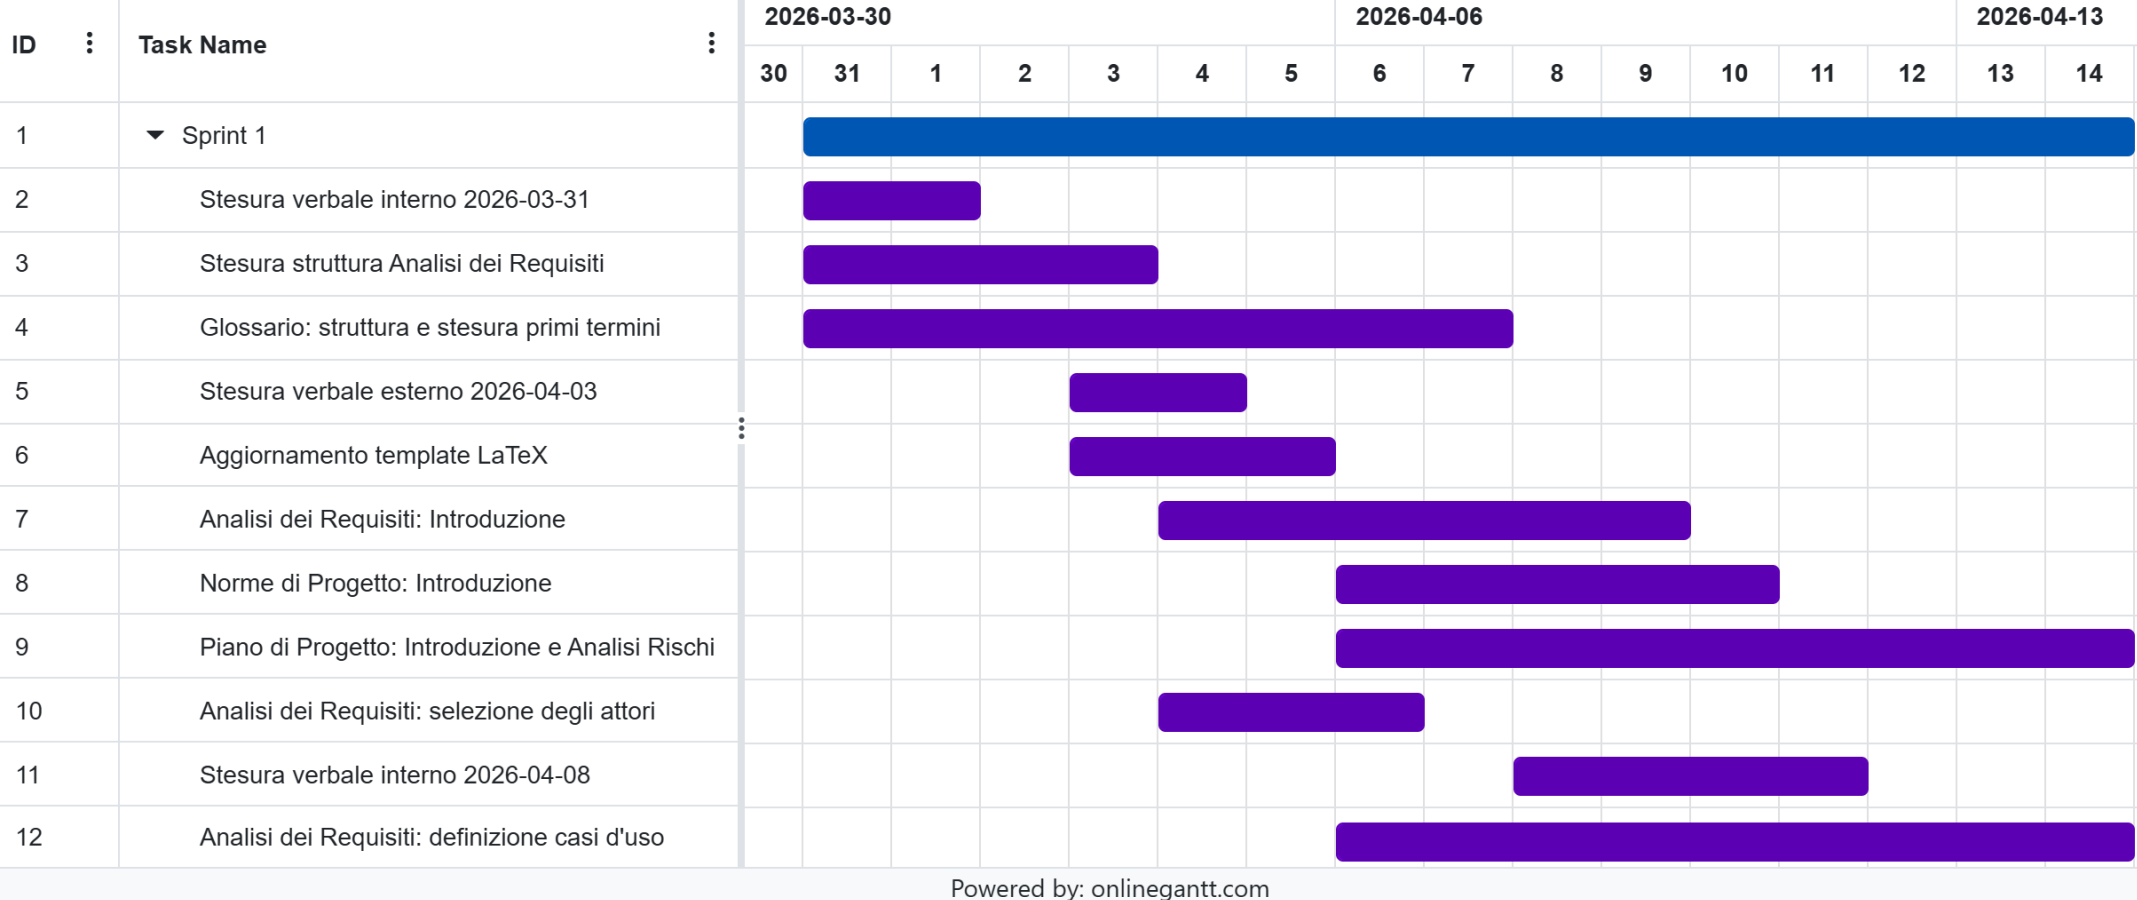
\includegraphics[width=\textwidth]{assets/gantt-sprint-1.png}
    \caption{Diagramma di Gantt dello Sprint 1}
    \label{fig:gantt-sprint1}
\end{figure}

\subsection{Sprint \#2: da 2026-04-14 a 2026-04-27}

\subsubsection{Obiettivi}
Durante il secondo sprint, il team prevede di consolidare e aggiornare la documentazione prodotta nello sprint\textsubscript{G} precedente, con particolare attenzione all'avanzamento dell'\textit{Analisi dei Requisiti}. L'obiettivo principale è passare dalla fase preliminare di studio e modellazione alla stesura più formale dei casi d'uso\textsubscript{G}, mantenendo allineati il \textit{Piano di Progetto}, le \textit{Norme di Progetto}, il \textit{Glossario} e l'\textit{Analisi dei Requisiti}.
Nello specifico, il team si impegnerà a:
\begin{itemize}
    \item proseguire la stesura del documento \textit{Analisi dei Requisiti}, avviando la descrizione formale dei casi d'uso\textsubscript{G} precedentemente studiati e modellati;

    \item completare la prima versione delle \textit{Norme di Progetto}, così da fornire al gruppo una base normativa condivisa per la gestione del lavoro, della documentazione e degli strumenti utilizzati;

    \item completare, all'interno del \textit{Piano di Progetto}, la sezione relativa all'analisi e alla gestione dei rischi e redigere il consuntivo e la retrospettiva dello Sprint\textsubscript{G} \#1, analizzando gli scostamenti rispetto al preventivo e individuando eventuali azioni correttive;

    \item aggiornare il \textit{Glossario} con i termini tecnici emersi durante la stesura della documentazione e durante le attività di analisi;

    \item avviare un'attività di brainstorming per il design preliminare UX/UI\textsubscript{G}, in vista della preparazione del mock-up\textsubscript{G} previsto per lo Sprint\textsubscript{G} \#3;

    \item redigere i verbali interni ed esterni relativi agli incontri svolti durante lo sprint\textsubscript{G}.
\end{itemize}

\begin{figure}[H]
    \centering
    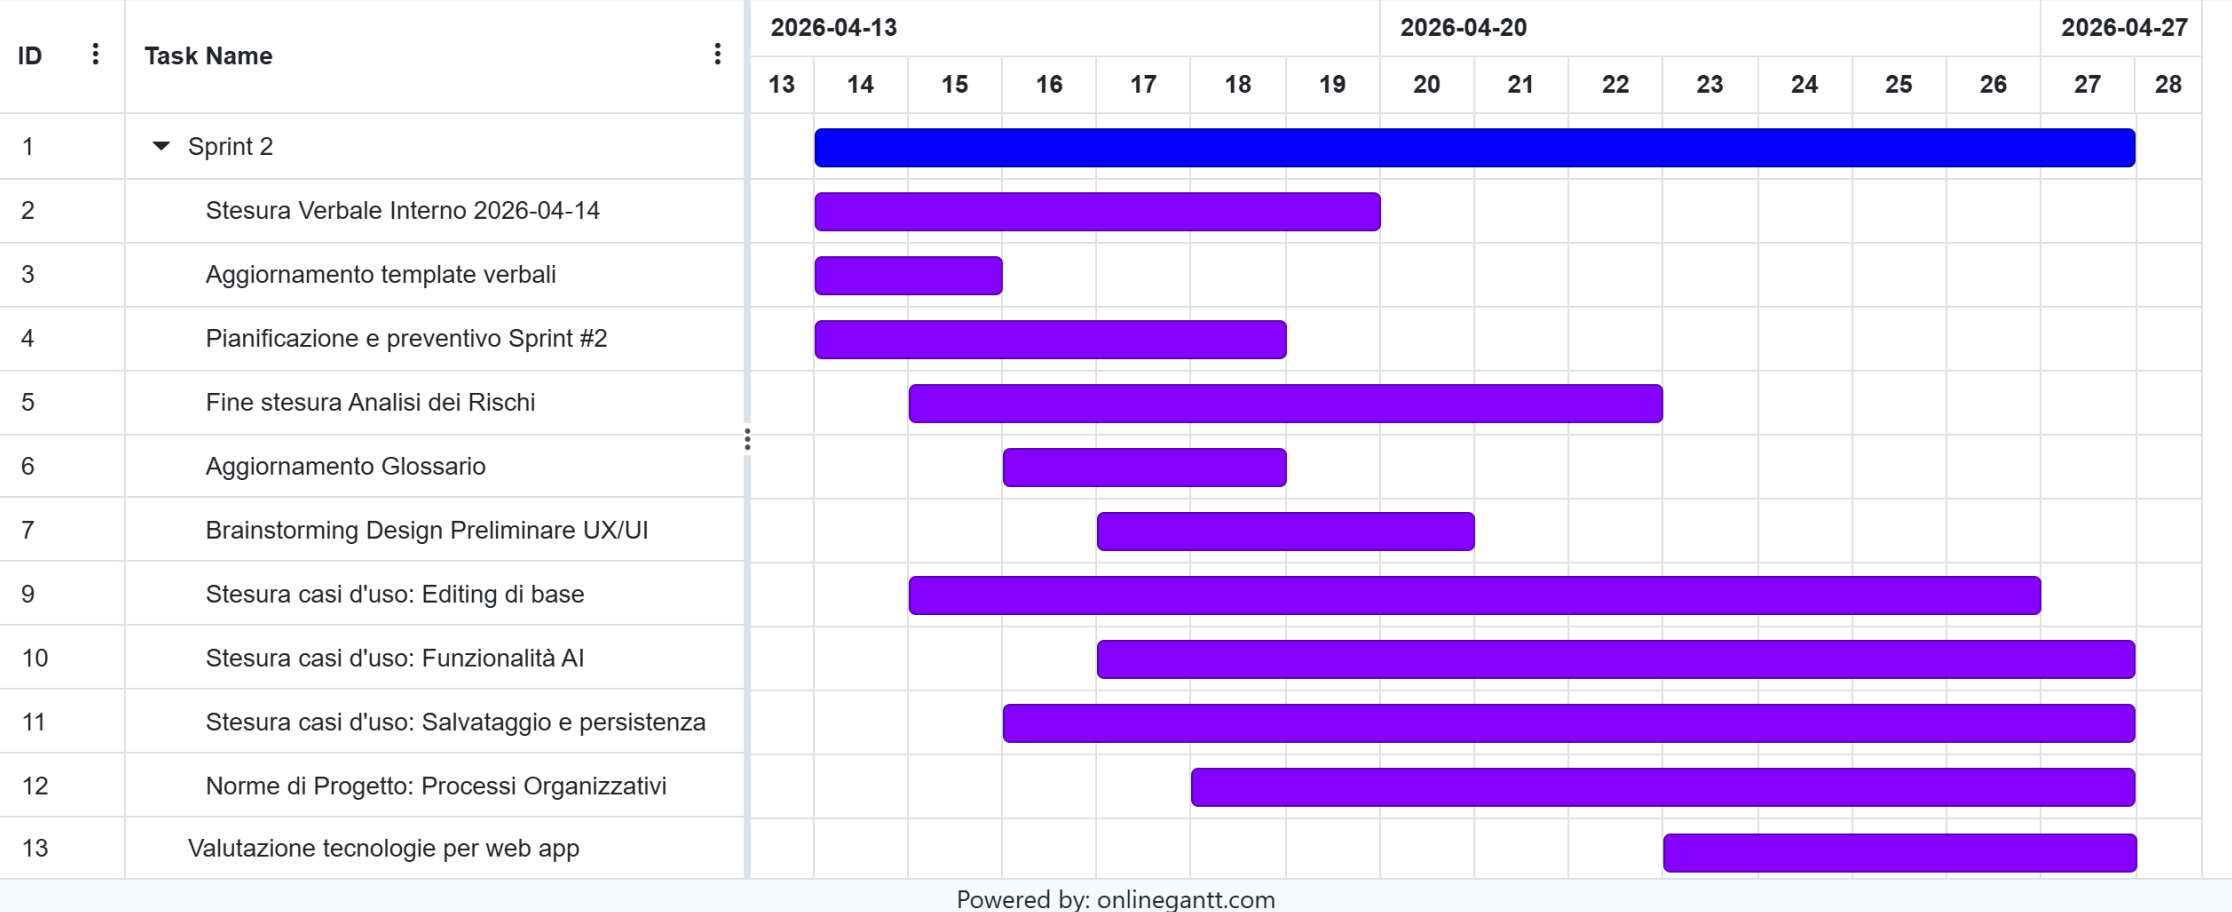
\includegraphics[width=\textwidth]{assets/gantt-sprint-2.png}
    \caption{Diagramma di Gantt dello Sprint 2}
    \label{fig:gantt-sprint2}
\end{figure}

\subsection{Sprint \#3: da 2026-04-28 a 2026-05-11}
\subsubsection{Obiettivi}
Durante il terzo sprint\textsubscript{G}, il team prevede di concentrare le attività sul completamento dell'\textit{Analisi dei Requisiti} e sull'avvio delle prime attività progettuali legate al prodotto software. 
In questo sprint\textsubscript{G} viene inoltre introdotto il ruolo di Progettista, principalmente per la realizzazione del mock-up\textsubscript{G} dell'interfaccia utente e per le prime attività di raccordo tra requisiti, esperienza utente e futura implementazione del prodotto.
Nello specifico, il team si impegnerà a:
\begin{itemize}
    \item completare l'\textit{Analisi dei Requisiti}, realizzando i diagrammi UML\textsubscript{G} relativi ai casi d'uso\textsubscript{G};

    \item organizzare un incontro con la Proponente\textsubscript{G} per discutere i casi d'uso individuati, chiarire eventuali ambiguità e ottenere un riscontro prima di procedere con le fasi successive del progetto;

    \item avviare la realizzazione del mock-up\textsubscript{G} dell'interfaccia utente, definendo una prima rappresentazione grafica delle principali schermate e dei flussi di interazione dell'applicazione;

    \item svolgere uno studio iniziale delle tecnologie da adottare nello sviluppo del prodotto software, valutando quali strumenti risultino più adeguati per la realizzazione della web app\textsubscript{G};

    \item proseguire l'aggiornamento dei documenti di progetto, in particolare \textit{Piano di Progetto}, \textit{Norme di Progetto}, \textit{Glossario} e \textit{Analisi dei Requisiti};

    \item sviluppare uno script\textsubscript{G} per automatizzare la gestione dei termini del \textit{Glossario}, riducendo il lavoro manuale necessario per inserire nei documenti il riferimento ai termini glossarizzati;
    \item redigere i verbali interni ed esterni relativi agli incontri svolti durante lo sprint\textsubscript{G}.
\end{itemize}

\begin{figure}[H]
    \centering
    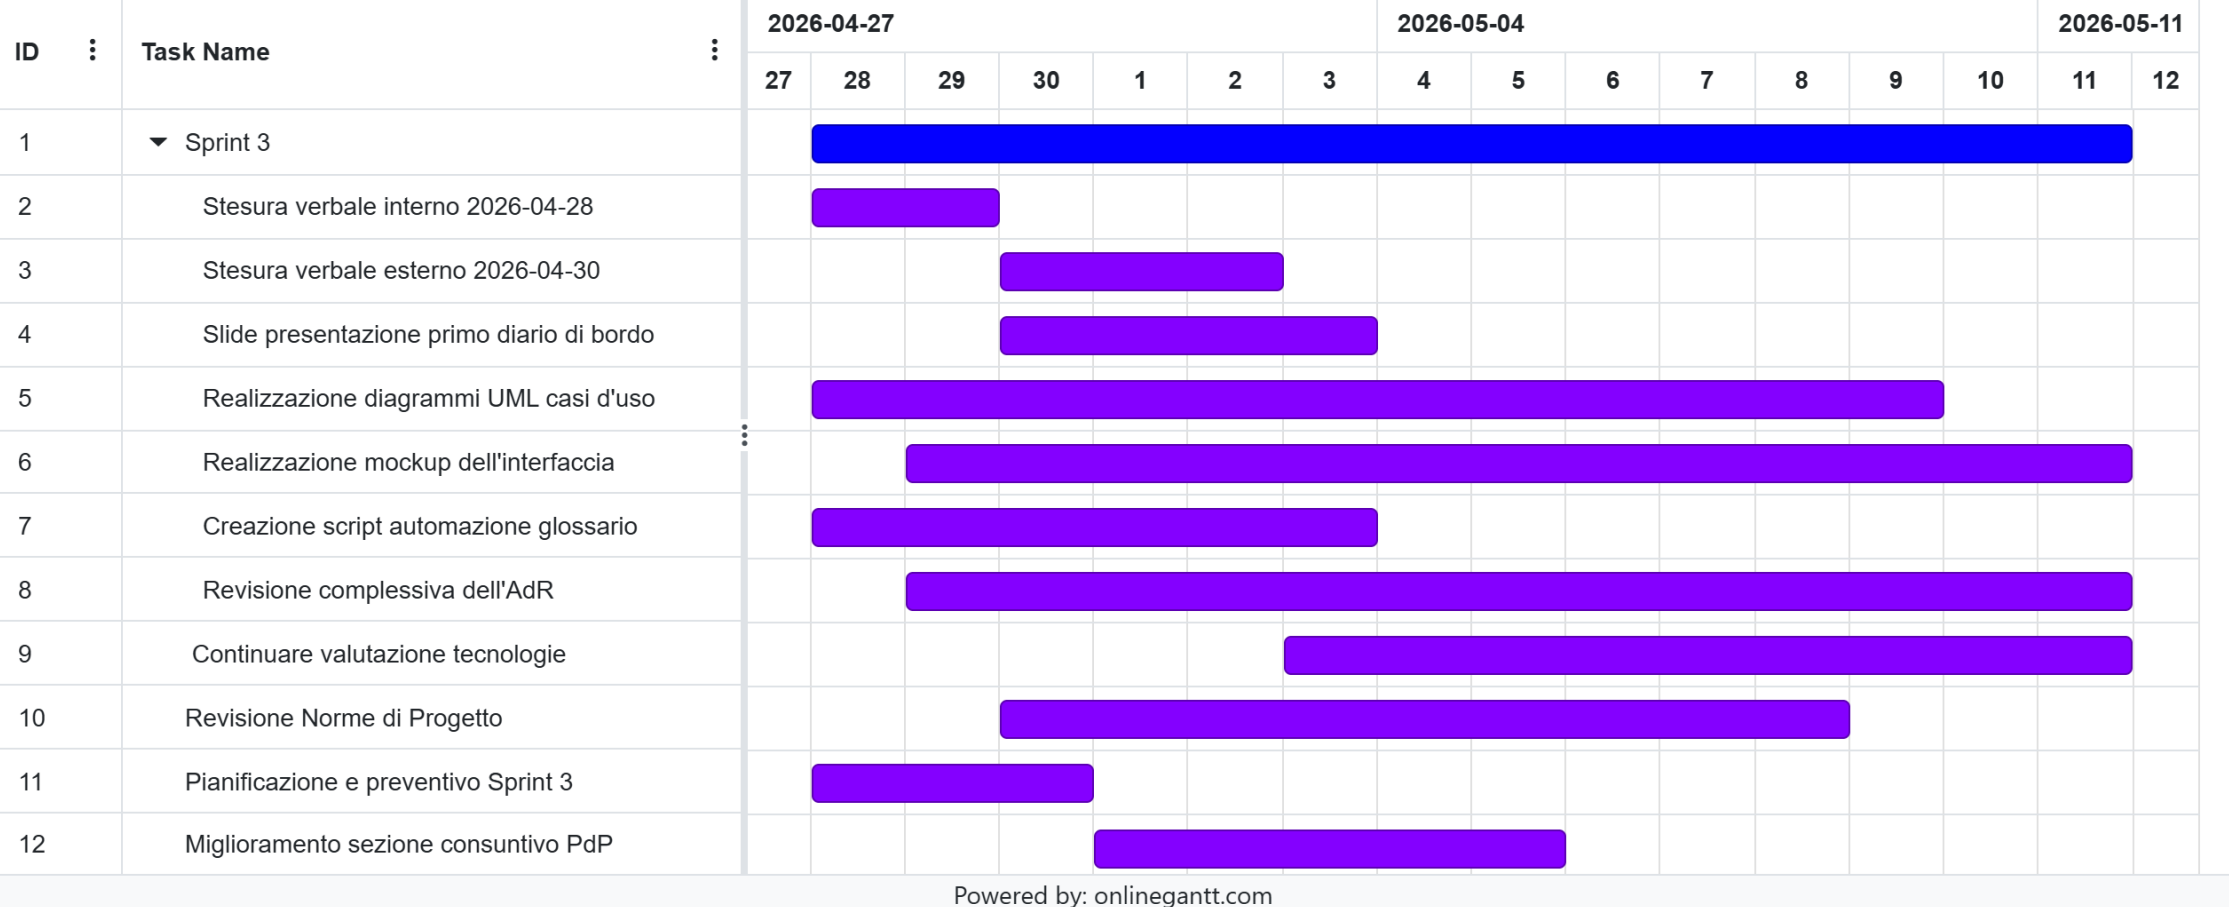
\includegraphics[width=\textwidth]{assets/gantt-sprint-3.png}
    \caption{Diagramma di Gantt dello Sprint 3}
    \label{fig:gantt-sprint3}
\end{figure}


\subsection{Sprint \#4: da 2026-05-12 a 2026-05-25}

\subsubsection{Obiettivi}

Durante il quarto sprint\textsubscript{G}, il team prevede di concentrarsi principalmente sulla realizzazione del \textit{Proof of Concept} e sulla definizione dell'architettura logica necessaria a supportare le funzionalità richieste dal capitolato C6 - \textit{Second Brain}.
\begin{itemize}
    \item consolidare definitivamente il documento di Analisi dei Requisiti in ogni sua sezione;
    \item prendere le decisioni formali e definitive sullo stack tecnologico e sui framework da adottare per lo sviluppo del \textit{Proof of Concept} e del prodotto software finale;
    \item avviare uno studio iniziale per definire l'architettura logica del PoC e comprendere i requisiti minimi necessari alla sua progettazione;
    \item introdurre formalmente il ruolo di Programmatore, che lavorerà in sinergia con il Progettista per l'avvio delle attività tecniche legate al \textit{Proof of Concept};
    \item iniziare lo sviluppo e la codifica effettiva del PoC verso la conclusione dello sprint;
    \item avviare un percorso di formazione per allineare tutti i componenti del gruppo sulle tecnologie scelte;
    \item proseguire con l'aggiornamento e la stesura della documentazione di supporto.
\end{itemize}

\begin{figure}[H]
    \centering
    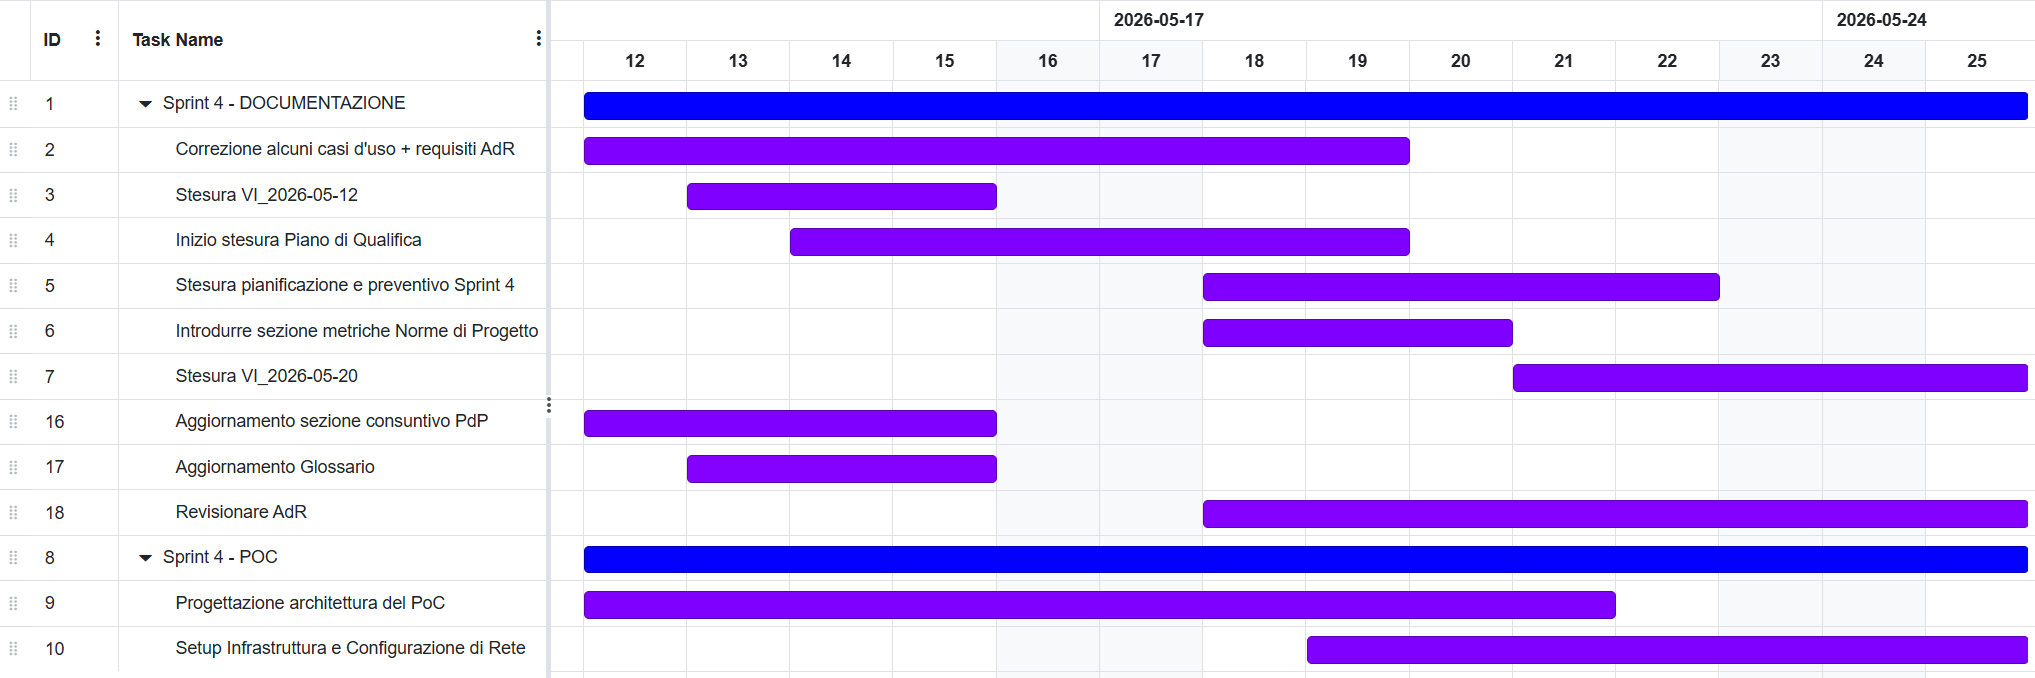
\includegraphics[width=\textwidth]{assets/gantt-sprint-4.png}
    \caption{Diagramma di Gantt dello Sprint 4}
    \label{fig:gantt-sprint4}
\end{figure}

\subsection{Sprint \#5: da 2026-05-26 a 2026-06-08}

\subsubsection{Obiettivi}
Gli obiettivi dello Sprint\textsubscript{G} \#5 sono stati definiti a partire dalle evidenze emerse nella retrospettiva precedente e in coerenza con l'avanzamento complessivo del progetto. L'attività centrale dell'iterazione è il completamento del \textit{Proof of Concept}, affiancata dalla stesura del \textit{Piano di Qualifica} e dalla revisione di correttezza dei documenti già prodotti.

Per concentrare l'impegno sullo sviluppo, il team ha previsto l'impiego di tre Programmatori\textsubscript{G}, dedicati in parallelo al front-end e al back-end del PoC, e di un Verificatore\textsubscript{G} incaricato di controllare in modo continuativo quanto via via implementato.

Nello specifico, il team si impegnerà a:
\begin{itemize}
    \item completare lo sviluppo del \textit{Proof of Concept}, portando a termine entro la finestra dello sprint\textsubscript{G} l'implementazione del front-end e del back-end e la verifica delle componenti realizzate;

    \item proseguire la stesura del \textit{Piano di Qualifica}, con particolare attenzione alla sezione dedicata alle metriche di prodotto, che saranno popolate a partire dai test\textsubscript{G} effettivamente eseguiti sul PoC: la disponibilità di codice funzionante consentirà di passare da definizioni astratte a misurazioni concrete;

    \item revisionare la correttezza dei documenti già prodotti, correggendo eventuali refusi, aggiornando i riferimenti incrociati e allineando i contenuti allo stato corrente del progetto, con particolare riguardo alle \textit{Norme di Progetto};

    \item aggiornare il \textit{Piano di Progetto} per riflettere i consuntivi dello Sprint\textsubscript{G} \#4 e la pianificazione rivista per gli sprint\textsubscript{G} successivi;

    \item avanzare il \textit{Glossario} con i nuovi termini emersi durante lo sviluppo e la progettazione, integrandolo nel sito pubblico del gruppo affinché risulti direttamente consultabile online;

    \item migliorare la veste grafica e l'organizzazione del sito pubblico del progetto;

    \item proseguire l'attività di studio e approfondimento delle tecnologie adottate per lo sviluppo del PoC;

    \item redigere i verbali interni ed esterni relativi agli incontri svolti durante lo sprint\textsubscript{G}.
\end{itemize}

\begin{figure}[H]
    \centering
    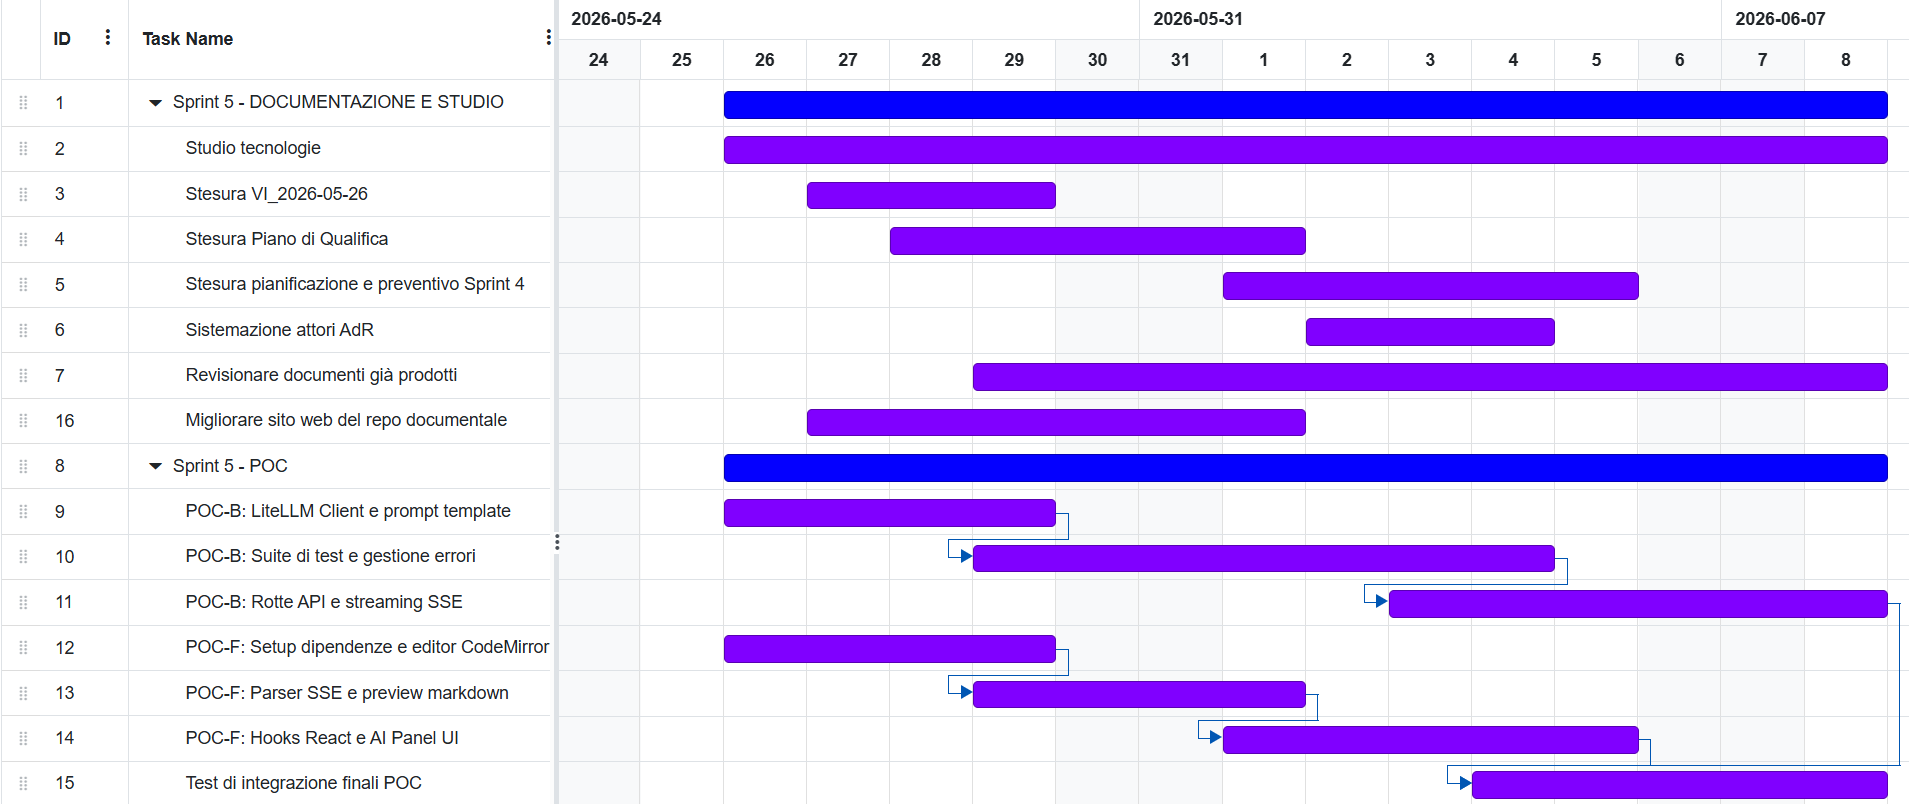
\includegraphics[width=\textwidth]{assets/gantt-sprint-5.png}
    \caption{Diagramma di Gantt dello Sprint 5}
    \label{fig:gantt-sprint5}
\end{figure}

\subsection{Sprint \#6: da 2026-06-09 a 2026-06-22}

\subsubsection{Obiettivi}
Lo Sprint\textsubscript{G} \#6 è dedicato principalmente ad attività di programmazione e di verifica\textsubscript{G}, in vista della presentazione della RTB\textsubscript{G}. L'obiettivo centrale è il completamento del \textit{Proof of Concept} e il controllo accurato di tutta la documentazione prodotta finora.

Nello specifico, il team si impegnerà a:
\begin{itemize}
    \item completare lo sviluppo del \textit{Proof of Concept};
    \item verificare accuratamente tutti i documenti in vista della presentazione della RTB\textsubscript{G}, con particolare attenzione all'\textit{Analisi dei Requisiti}, alle \textit{Norme di Progetto} e al \textit{Piano di Progetto};
    \item completare il \textit{Piano di Qualifica} e sottoporlo a un'accurata verifica\textsubscript{G};
    \item organizzare un incontro con la Proponente\textsubscript{G} per mostrare il \textit{Proof of Concept} e raccoglierne il riscontro;
    \item preparare le diapositive per la presentazione RTB\textsubscript{G} delle tecnologie;
    \item redigere la lettera di presentazione destinata al prof. Cardin;
    \item richiedere al prof. Cardin il colloquio per la presentazione delle tecnologie della RTB\textsubscript{G};
    \item redigere i verbali interni ed esterni relativi agli incontri svolti durante lo sprint\textsubscript{G}.
\end{itemize}

\begin{figure}[H]
    \centering
    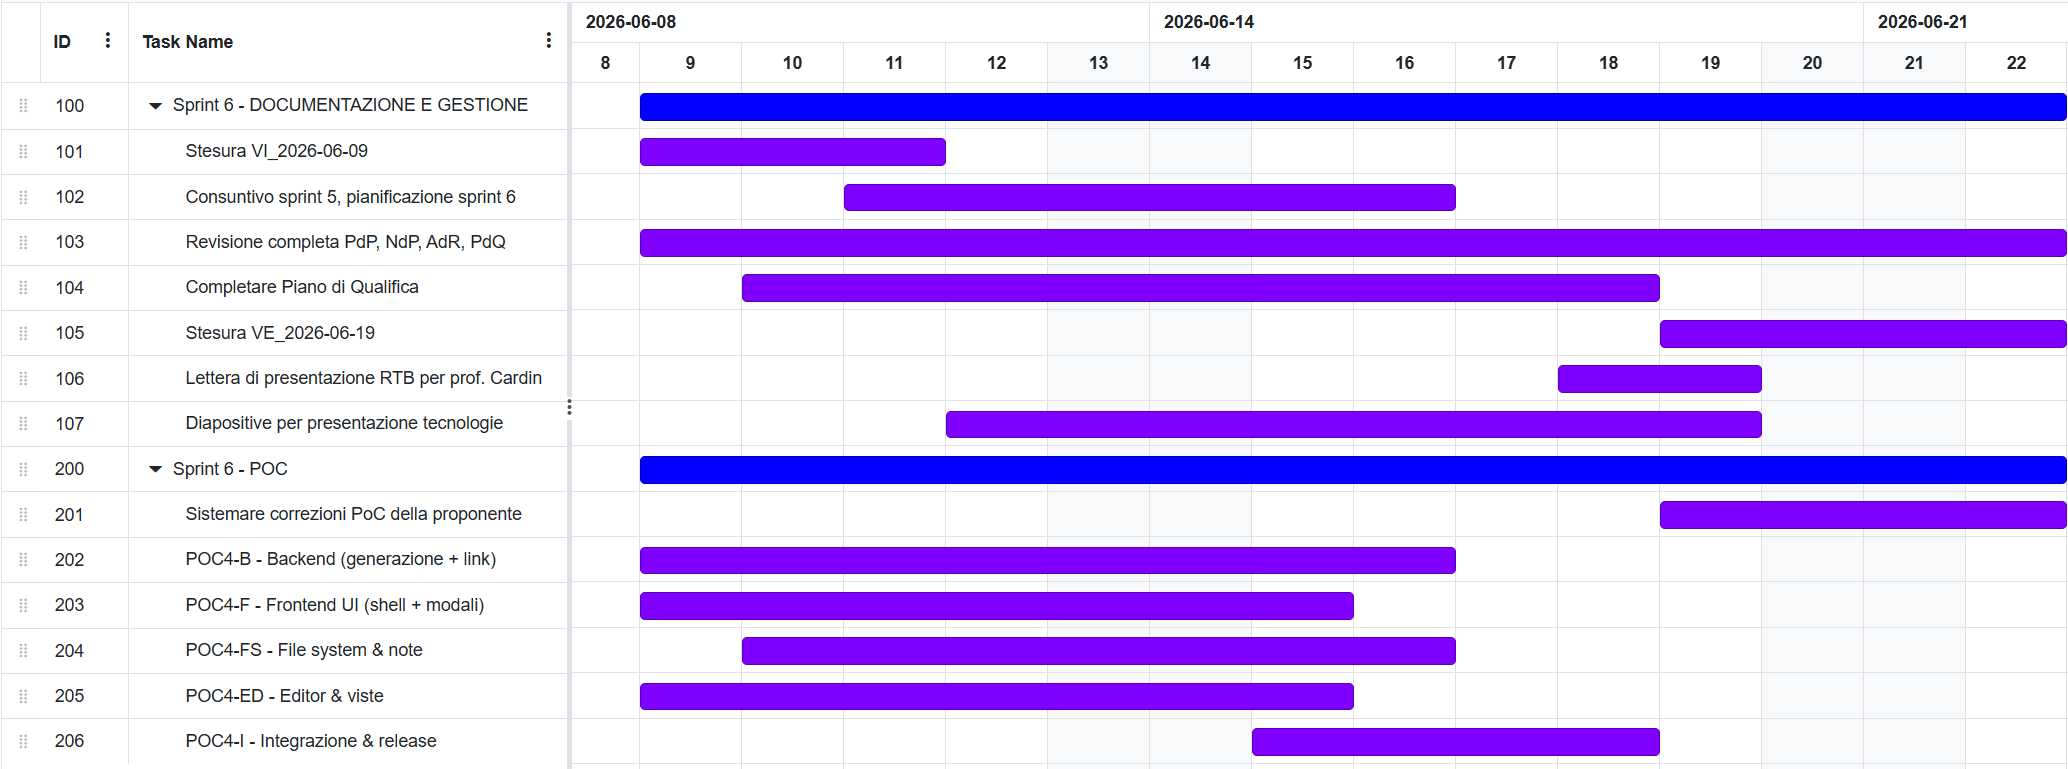
\includegraphics[width=\textwidth]{assets/gantt-sprint-6.png}
    \caption{Diagramma di Gantt dello Sprint 6}
    \label{fig:gantt-sprint6}
\end{figure}

\subsection{Sprint \#7: da 2026-06-23 a 2026-07-06}

\subsubsection{Obiettivi}
Lo Sprint\textsubscript{G} \#7 comprende la consegna della RTB\textsubscript{G}, avvenuta il 25 giugno 2026 con circa cinque giorni di ritardo rispetto a quanto pianificato per lo Sprint\textsubscript{G} \#6, ed è dedicato alla formalizzazione della candidatura per la presentazione delle tecnologie, all'attesa del riscontro da parte del prof. Cardin e al consolidamento della documentazione, oltre a un'intensa attività di palestra in preparazione della fase successiva di Progettazione e Codifica.

Nello specifico, il team si impegnerà a:
\begin{itemize}
    \item inoltrare al prof. Cardin la candidatura per il colloquio di presentazione delle tecnologie della RTB\textsubscript{G}, svolgere la relativa presentazione e attenderne il riscontro;
    \item redigere la lettera di presentazione della RTB\textsubscript{G} destinata al prof. Vardanega;
    \item aggiornare i documenti soggetti a modifica, in particolare il \textit{Piano di Progetto} (con l'aggiunta del consuntivo dello Sprint\textsubscript{G} \#6 e della pianificazione e del preventivo dello Sprint\textsubscript{G} \#7) e il \textit{Piano di Qualifica} (con l'aggiunta degli Sprint\textsubscript{G} \#6 e \#7);
    \item approvare tutti i documenti per l'ingresso nella baseline\textsubscript{G} della RTB\textsubscript{G};
    \item avviare la progettazione dell'MVP\textsubscript{G}, limitatamente alla progettazione e senza attività di codifica;
    \item analizzare i documenti da produrre nella fase di Product Baseline\textsubscript{G}, in particolare il \textit{Manuale Utente} e la \textit{Specifica Tecnica};
    \item dedicare ore di palestra all'approfondimento delle tecnologie e alla preparazione delle attività iniziali della Product Baseline\textsubscript{G}.
\end{itemize}

Il gruppo attribuisce particolare importanza alle ore di palestra: prima di avviare concretamente le attività di sviluppo è infatti fondamentale comprendere \textit{come} realizzarle. Si tratta di ore che non vengono rendicontate come effettivamente produttive, ma che risultano essenziali per costruire una base solida su cui impostare il lavoro della fase successiva.

\begin{figure}[H]
    \centering
    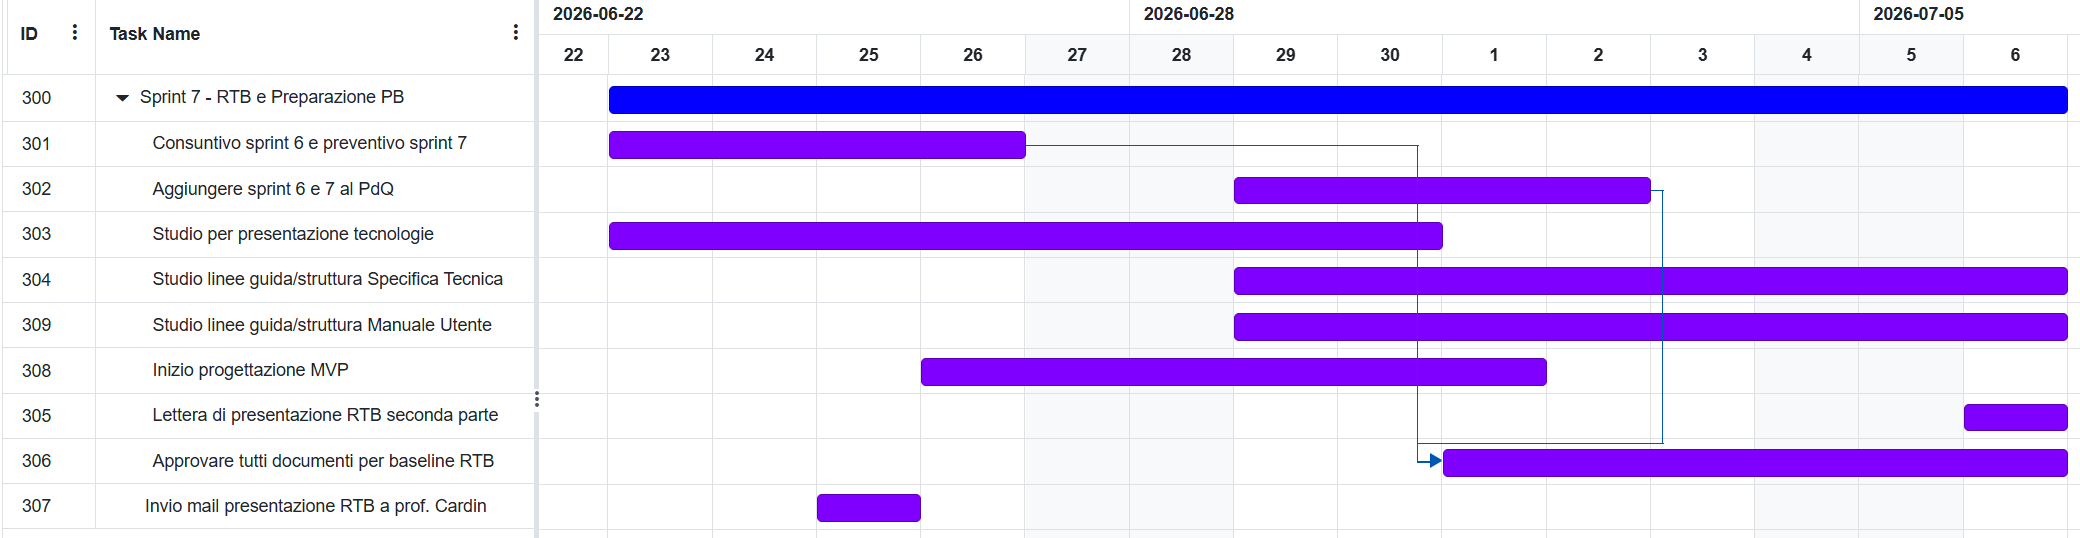
\includegraphics[width=\textwidth]{assets/gantt-sprint-7.png}
    \caption{Diagramma di Gantt dello Sprint 7}
    \label{fig:gantt-sprint7}
\end{figure}

\subsection{Sprint \#8: da 2026-07-07 a 2026-07-20}

\subsubsection{Obiettivi}
Lo Sprint\textsubscript{G} \#8 rappresenta il punto di passaggio tra la fase di RTB\textsubscript{G} e quella di Product Baseline\textsubscript{G}. Il periodo è dedicato al recepimento dei rilievi mossi dal prof. Riccardo Cardin sull'\textit{Analisi dei Requisiti}, alla preparazione e allo svolgimento della seconda parte della presentazione RTB\textsubscript{G} con il prof. Tullio Vardanega e, a valle dell'esito positivo di tale incontro, all'ingresso effettivo nella fase di PB\textsubscript{G}.

Il monte ore preventivato\textsubscript{G} per il periodo, pari a 63 ore, è sensibilmente superiore alla media degli sprint\textsubscript{G} precedenti. La decisione, assunta durante la riunione di apertura dello sprint\textsubscript{G} del 2026-07-07, nasce dalla concentrazione in un unico periodo di tre attività onerose e in larga parte parallele. A ciò si aggiunge una scelta di metodo: avendo constatato negli sprint\textsubscript{G} precedenti che i ruoli affidati a una sola persona sono esposti alle variazioni di disponibilità individuale, il gruppo ha ripartito i tre ruoli più carichi su tre membri ciascuno, accettando un monte ore complessivo più alto in cambio di un margine interno di manovra.

Nello specifico, il team si impegnerà a:
\begin{itemize}
    \item sistemare gli errori e i requisiti\textsubscript{G} segnalati dal prof. Riccardo Cardin nell'\textit{Analisi dei Requisiti}, con particolare attenzione ai requisiti\textsubscript{G} non funzionali, rendendoli più chiari, misurabili e verificabili\textsubscript{G};

    \item svolgere le attività di studio e preparazione, sia individuali sia collettive, in vista dell'incontro con il prof. Tullio Vardanega, così da presentarsi con una comprensione uniforme e condivisa del lavoro svolto;

    \item predisporre i materiali e le argomentazioni da esporre al prof. Tullio Vardanega durante la seconda parte della presentazione RTB\textsubscript{G}, prevista per il 9 luglio 2026;

    \item avviare la fase di Product Baseline\textsubscript{G} a seguito dell'incontro con il prof. Tullio Vardanega, impostando le attività e i documenti che ne costituiscono l'oggetto;

    \item avviare, da parte dei Progettisti\textsubscript{G}, la progettazione\textsubscript{G} di dettaglio dell'MVP\textsubscript{G} a partire dalle scelte già consolidate nel \textit{Proof of Concept};

    \item analizzare i design pattern\textsubscript{G} e l'architettura\textsubscript{G} generale del prodotto, motivandone le scelte e avviandone la stesura all'interno del documento di \textit{Specifica Tecnica}.
\end{itemize}

Per sostenere queste attività il gruppo ha previsto due Analisti\textsubscript{G}, incaricati della revisione incrociata dei requisiti\textsubscript{G}, e due Progettisti\textsubscript{G}, dedicati in parallelo alla progettazione\textsubscript{G} dell'MVP\textsubscript{G} e allo studio dei pattern\textsubscript{G} architetturali. Non è invece previsto alcun Programmatore\textsubscript{G}: la progettazione\textsubscript{G} è ancora in fase di avvio e non fornisce una base sufficientemente matura per iniziare la codifica\textsubscript{G}.

\subsection{Sprint \#9: da 2026-07-21 a 2026-08-03}

\subsubsection{Obiettivi}
Lo Sprint\textsubscript{G} \#9 segna il passaggio dalla sola progettazione\textsubscript{G} alla codifica\textsubscript{G} vera e propria: la progettazione\textsubscript{G} di dettaglio avviata nel periodo precedente ha raggiunto un grado di maturità sufficiente a fornire ai Programmatori\textsubscript{G} una base implementabile, e il gruppo avvia pertanto l'implementazione\textsubscript{G} dell'MVP\textsubscript{G}. Il periodo è inoltre dedicato al recepimento dei riscontri ricevuti sulla valutazione dei documenti e della presentazione RTB\textsubscript{G}, che hanno evidenziato due interventi correttivi da applicare al processo documentale: la revisione delle \textit{Norme di Progetto} in chiave procedurale e la correzione dell'uso del registro delle modifiche\textsubscript{G}.

Nello specifico, il team si impegnerà a:
\begin{itemize}
    \item proseguire la progettazione\textsubscript{G} di dettaglio dell'MVP\textsubscript{G}, dando continuità al lavoro avviato nello Sprint\textsubscript{G} \#8 a partire dalle scelte già consolidate nel \textit{Proof of Concept};

    \item avviare l'implementazione\textsubscript{G} effettiva dell'MVP\textsubscript{G} sulla base degli artefatti\textsubscript{G} prodotti dai Progettisti\textsubscript{G}, traducendo in codice le decisioni architetturali già assunte;

    \item migliorare il documento \textit{Norme di Progetto} a seguito del riscontro ricevuto, riscrivendone le parti interessate in forma procedurale anziché descrittiva, così che il documento guidi operativamente lo svolgimento delle attività invece di limitarsi a raccontarle;

    \item redigere i verbali\textsubscript{G} interni delle riunioni del periodo, secondo quanto previsto dalle \textit{Norme di Progetto};

    \item comprendere l'errore commesso nella compilazione del campo \textit{Approvatore} del registro delle modifiche\textsubscript{G} e correggerlo in modo sistematico su tutti i documenti soggetti a versionamento\textsubscript{G}, ripristinando la corretta distinzione fra le attività di stesura, verifica\textsubscript{G} e approvazione\textsubscript{G};

    \item avviare la stesura del documento di \textit{Specifica Tecnica}, redigendone l'introduzione e la definizione dell'architettura\textsubscript{G} del prodotto con le relative scelte architetturali;

    \item condurre, da parte dei Progettisti\textsubscript{G}, un'attività di brainstorming\textsubscript{G} e di definizione decisionale dei design pattern\textsubscript{G} e dei pattern\textsubscript{G} architetturali da adottare, motivando il \emph{perché} di ciascuna scelta come fase preparatoria alla stesura completa del documento;

    \item aggiornare il \textit{Piano di Progetto} con il consuntivo\textsubscript{G} dello Sprint\textsubscript{G} \#8 e con la pianificazione\textsubscript{G} e il preventivo\textsubscript{G} dello Sprint\textsubscript{G} \#9.
\end{itemize}

La composizione dei ruoli recepisce quanto stabilito nella riunione di apertura dello sprint\textsubscript{G} del 2026-07-21: il gruppo introduce \textbf{due Programmatori\textsubscript{G}}, poiché l'implementazione\textsubscript{G} dell'MVP\textsubscript{G} è un'attività onerosa che beneficia di due figure dedicate, e mantiene in parallelo \textbf{due Progettisti\textsubscript{G}}, incaricati di proseguire la progettazione\textsubscript{G} di dettaglio e la definizione dei pattern\textsubscript{G} architetturali così da alimentare senza interruzioni il lavoro dei Programmatori\textsubscript{G}. Non è invece previsto alcun Analista\textsubscript{G}: i requisiti\textsubscript{G} sono stati stabilizzati nello Sprint\textsubscript{G} \#8 a valle dei rilievi del prof. Riccardo Cardin e non necessitano di ulteriori interventi in questo periodo.

Il periodo coincide inoltre con l'inizio delle vacanze estive e diversi membri hanno dichiarato una disponibilità ridotta. Per garantire comunque la copertura delle attività di verifica\textsubscript{G}, che con l'avvio della codifica\textsubscript{G} si estendono dal solo piano documentale a quello del codice, il gruppo ha stabilito che \textbf{S. Vendramin ricopra contemporaneamente i ruoli di Responsabile\textsubscript{G} e di Verificatore\textsubscript{G}}, affiancando A. Menegaldo nella revisione degli artefatti\textsubscript{G} prodotti. L'attività di correzione dei registri delle modifiche\textsubscript{G} e la revisione delle \textit{Norme di Progetto} restano affidate all'Amministratore\textsubscript{G} con il supporto del Responsabile\textsubscript{G}, trattandosi di interventi sul processo e sulla configurazione\textsubscript{G} e non sul prodotto.

\subsection{Sprint \#10: da 2026-08-04 a 2026-08-10}

\subsubsection{Obiettivi}
Lo Sprint\textsubscript{G} \#10 è il primo periodo di durata pari a una sola settimana. La riduzione, deliberata nella riunione di apertura del 2026-08-04, risponde all'esigenza di concentrare le attività nel minor tempo possibile: con l'incontro con il prof. Riccardo Cardin atteso intorno al 20-21 agosto e la successiva consegna finale al prof. Tullio Vardanega, una cadenza settimanale consente al gruppo di mantenere il focus sugli obiettivi, di coordinarsi più agilmente e di evitare i tempi morti che una finestra di quattordici giorni comporterebbe in questa fase conclusiva.

L'obiettivo centrale del periodo è il \textbf{completamento del codice dell'MVP\textsubscript{G}}. La scelta è strategica prima ancora che operativa: portare a termine l'applicativo in questo sprint\textsubscript{G} è la condizione necessaria per dedicare il periodo successivo alla sola documentazione. Diverse attività documentali ancora aperte, in primo luogo le schermate da inserire nel \textit{Manuale Utente}, presuppongono infatti un sistema in configurazione\textsubscript{G} definitiva: produrle su una base di codice ancora in evoluzione comporterebbe doverle rifare a valle di ogni modifica.

Nello specifico, il team si impegnerà a:
\begin{itemize}
    \item completare l'implementazione\textsubscript{G} dell'MVP\textsubscript{G}, portando a termine i moduli\textsubscript{G} ancora aperti e le integrazioni fra front-end e back-end;

    \item avviare la stesura del \textit{Manuale Utente}, redigendone l'introduzione e le sezioni iniziali;

    \item redigere la sezione dedicata all'architettura\textsubscript{G} e ai design pattern\textsubscript{G} all'interno del documento di \textit{Specifica Tecnica}, formalizzando le scelte assunte nella riunione di apertura dello sprint\textsubscript{G};

    \item aggiornare il \textit{Piano di Progetto} con il consuntivo\textsubscript{G} dello Sprint\textsubscript{G} \#9 e con la pianificazione\textsubscript{G} e il preventivo\textsubscript{G} dello Sprint\textsubscript{G} \#10;

    \item aggiornare il \textit{Piano di Qualifica} in base all'avanzamento della codifica\textsubscript{G} e delle attività di verifica\textsubscript{G};

    \item redigere e inviare il nuovo Diario di Bordo\textsubscript{G};

    \item redigere il verbale\textsubscript{G} interno della riunione del periodo, secondo quanto previsto dalle \textit{Norme di Progetto}.
\end{itemize}

La composizione dei ruoli recepisce quanto stabilito nella riunione di apertura dello sprint\textsubscript{G}. Il gruppo porta a \textbf{tre i Programmatori\textsubscript{G}}, coerentemente con l'obiettivo di chiudere la codifica\textsubscript{G} entro il periodo, e mantiene \textbf{due Progettisti\textsubscript{G}}, incaricati sia della stesura della sezione architetturale della \textit{Specifica Tecnica} sia del supporto ai Programmatori\textsubscript{G} sui punti di progettazione\textsubscript{G} che dovessero emergere in fase di sviluppo. Il ruolo Analista\textsubscript{G} resta a zero ore, essendo i requisiti\textsubscript{G} stabilizzati dallo Sprint\textsubscript{G} \#8.

La novità più rilevante riguarda il ruolo Verificatore\textsubscript{G}, che viene \textbf{ripartito su quattro membri} anziché concentrato su una o due figure come nei periodi precedenti. La scelta risponde direttamente al rischio\textsubscript{G} RT-3 (\textit{Presenza di errori nel codice}), la cui pericolosità era stata elevata ad \textit{Alta} al termine dello Sprint\textsubscript{G} \#9: con la codifica\textsubscript{G} in fase di completamento il volume di codice da sottoporre a revisione cresce sensibilmente e il gruppo ha preferito distribuire la capacità di verifica\textsubscript{G} su più persone, così da poterla incrementare in corso di sprint\textsubscript{G} qualora il rischio\textsubscript{G} si manifestasse.

Per sostenere questa composizione \textbf{quattro membri ricoprono un doppio ruolo\textsubscript{G}}. S. Zecchinato affianca al ruolo di Responsabile\textsubscript{G} quello di Programmatore\textsubscript{G}, destinando alla codifica\textsubscript{G} le ore eccedenti quelle di coordinamento; E. De Piccoli affianca all'Amministratore\textsubscript{G} il ruolo di Verificatore\textsubscript{G}, poiché le attività di configurazione\textsubscript{G} e di gestione dei rilasci hanno ormai carattere consolidato e non assorbono l'intero monte ore del ruolo; L. Battistella e D. Facco affiancano alla progettazione\textsubscript{G} una quota di verifica\textsubscript{G}, potendo così controllare la corrispondenza fra il codice prodotto e gli artefatti\textsubscript{G} architetturali di cui sono autori. La misura recepisce l'indicazione della retrospettiva\textsubscript{G} dello Sprint\textsubscript{G} \#9, che aveva formalizzato il supporto fuori ruolo\textsubscript{G} come criterio di pianificazione\textsubscript{G} anziché come rimedio adottato in corso d'opera.

\subsection{Sprint \#11: da 2026-08-11 a 2026-08-17}

\subsubsection{Obiettivi}
Lo Sprint\textsubscript{G} \#11 chiude la produzione di prodotto e documentazione e mantiene la cadenza settimanale dello Sprint\textsubscript{G} \#10. Non sono previste nuove funzionalità: il periodo è dedicato al \textbf{consolidamento del prodotto e al completamento della documentazione}, in vista dell'incontro con il prof. Riccardo Cardin e della consegna finale al prof. Tullio Vardanega. Ogni artefatto\textsubscript{G} viene allineato allo stato effettivo dell'MVP\textsubscript{G} e verificato prima della chiusura del periodo.

Al periodo seguirà lo Sprint\textsubscript{G} \#12, dedicato alla preparazione e allo svolgimento delle presentazioni finali. Il preventivo\textsubscript{G} dello Sprint\textsubscript{G} \#11 tiene conto di tale fabbisogno e non impegna l'intero budget residuo: su ogni ruolo\textsubscript{G} viene lasciata disponibilità, per un totale di 15 ore, pari a 275,00 €.

Nello specifico, il team si impegnerà a:
\begin{itemize}
    \item completare l'implementazione\textsubscript{G} del codice dell'MVP\textsubscript{G}, limitandosi alla correzione dei difetti emersi in fase di verifica\textsubscript{G} e portando a termine gli ultimi test\textsubscript{G} funzionali sul prodotto;

    \item terminare la stesura del documento di \textit{Specifica Tecnica}, completando le sezioni ancora aperte e i diagrammi UML\textsubscript{G} necessari a rappresentare l'architettura\textsubscript{G} e il comportamento del sistema;

    \item terminare il \textit{Manuale Utente}, integrando le sezioni mancanti e le schermate del prodotto in configurazione\textsubscript{G} definitiva;

    \item aggiornare il \textit{Piano di Progetto} e il \textit{Piano di Qualifica} allo stato attuale del progetto, con il consuntivo\textsubscript{G} dello Sprint\textsubscript{G} \#10 e con la pianificazione\textsubscript{G} e il preventivo\textsubscript{G} dello Sprint\textsubscript{G} \#11;

    \item \textbf{verificare accuratamente tutti i documenti} destinati alla Product Baseline\textsubscript{G}, controllandone correttezza dei contenuti, coerenza reciproca, tracciamento\textsubscript{G} e conformità alle \textit{Norme di Progetto};

    \item aggiornare il sito web del gruppo con la rappresentazione della Product Baseline\textsubscript{G} e con la vista web del \textit{Manuale Utente};

    \item contattare la Proponente\textsubscript{G} per richiedere un incontro di presentazione del prodotto finale;

    \item redigere il verbale\textsubscript{G} interno della riunione del periodo, secondo quanto previsto dalle \textit{Norme di Progetto}.
\end{itemize}

\section{Preventivo}
Il preventivo viene elaborato considerando il costo orario associato a ciascun ruolo, il budget complessivo previsto e le attività pianificate per il periodo di riferimento. Per ogni sprint\textsubscript{G} vengono quindi riportati:

\begin{itemize}
    \item un preventivo delle ore previste, organizzato in forma tabellare;
    \item un preventivo dei costi stimati, anch'esso presentato in forma tabellare;
    \item un areogramma che rappresenta la distribuzione delle ore tra i diversi ruoli di progetto.
\end{itemize}

Il carico di lavoro complessivo previsto per ciascun componente del gruppo è pari a 89 ore, distribuite tra i diversi ruoli di progetto, per un totale di 623 ore produttive. La ripartizione delle mansioni viene gestita tramite un meccanismo di rotazione, con l'obiettivo di garantire a ogni membro del team la possibilità di ricoprire ruoli differenti e acquisire una visione più completa del processo di sviluppo.

Per rendere le tabelle più leggibili e compatte, i ruoli di progetto vengono indicati mediante le seguenti abbreviazioni\textsubscript{G}:

\begin{itemize}
    \item \textbf{Re}: Responsabile di progetto;
    \item \textbf{Am}: Amministratore;
    \item \textbf{An}: Analista;
    \item \textbf{Pt}: Progettista;
    \item \textbf{Pr}: Programmatore;
    \item \textbf{Ve}: Verificatore.
\end{itemize}

\subsection{Sprint \#1: da 2026-03-31 a 2026-04-13}
Di seguito è riportata la distribuzione delle ore per ciascun membro del team,
accumulate in totali per persona e per ruolo:

\begin{table}[H]
    \centering
    \renewcommand{\arraystretch}{1.4}
    \begin{tabular}{|l|c|c|c|c|c|c|c|}
        \hline
        \rowcolor{bluBitless!15}
        \textbf{Membro} & \textbf{Re} & \textbf{Am} & \textbf{An} & \textbf{Pt} & \textbf{Pr} & \textbf{Ve} & \textbf{Totale per persona} \\
        \hline
        L. Battistella & - & - & 6 & - & - & - & 6 \\ \hline
        E. De Piccoli & - & 5 & - & - & - & - & 5 \\ \hline
        D. Facco & - & - & 6 & - & - & - & 6 \\ \hline
        A. Marini & - & - & 6 & - & - & - & 6 \\ \hline
        A. Menegaldo & - & - & - & - & - & 8 & 8 \\ \hline
        S. Vendramin & 4 & - & - & - & - & - & 4 \\ \hline
        S. Zecchinato & - & - & 6 & - & - & - & 6 \\ \hline
        \rowcolor{bluBitless!8}
        \textbf{Totale per ruolo} & \textbf{4} & \textbf{5} & \textbf{24} & \textbf{-} & \textbf{-} & \textbf{8} & \textbf{41} \\
        \hline
    \end{tabular}
    \caption{\textit{Preventivo orario Sprint \#1}}
\end{table}

\begin{figure}[H]
\centering

\begin{tikzpicture}[scale=0.85]

% Colori pastello
\definecolor{colResp}{HTML}{BFE8DD}
\definecolor{colAmm}{HTML}{FFD0B5}
\definecolor{colAn}{HTML}{E4C9F5}
\definecolor{colVe}{HTML}{CDEBFF}
\definecolor{lineGray}{HTML}{8A8A8A}

% Raggio dell'areogramma
\def\r{3.2}

% Titolo
\node[font=\Large\bfseries] at (0,4.25) {Distribuzione ore per ruolo};

% Settori
% Totale = 41
% Re = 4 -> 9,8%
% Am = 5 -> 12,2%
% An = 24 -> 58,5%
% Ve = 8 -> 19,5%

\path[fill=colResp, draw=white, line width=1.5pt]
(0,0) -- (90:\r) arc[start angle=90,end angle=54.9,radius=\r] -- cycle;

\path[fill=colAmm, draw=white, line width=1.5pt]
(0,0) -- (54.9:\r) arc[start angle=54.9,end angle=11.0,radius=\r] -- cycle;

\path[fill=colAn, draw=white, line width=1.5pt]
(0,0) -- (11.0:\r) arc[start angle=11.0,end angle=-199.7,radius=\r] -- cycle;

\path[fill=colVe, draw=white, line width=1.5pt]
(0,0) -- (-199.7:\r) arc[start angle=-199.7,end angle=-270,radius=\r] -- cycle;

% Percentuali interne più piccole
\node[font=\normalsize\bfseries] at (70:1.75) {9,8\%};
\node[font=\normalsize\bfseries] at (31:1.85) {12,2\%};
\node[font=\normalsize\bfseries] at (-98:1.55) {58,5\%};
\node[font=\normalsize\bfseries] at (131:1.85) {19,5\%};

% Linee ed etichette esterne - Responsabile
\fill[lineGray] (1.25,2.75) circle (1.7pt);
\draw[lineGray, line width=0.7pt] (1.25,2.75) -- (3.65,2.75) -- (5.5,2.75);
\node[anchor=south east, font=\normalsize\bfseries] at (5.5,2.82) {Responsabile};
\node[anchor=north east, font=\small\bfseries, text=lineGray] at (5.5,2.60) {4 ore};

% Linee ed etichette esterne - Amministratore
\fill[lineGray] (2.85,1.05) circle (1.7pt);
\draw[lineGray, line width=0.7pt] (2.85,1.05) -- (4.0,1.05) -- (5.55,1.05);
\node[anchor=south east, font=\normalsize\bfseries] at (5.55,1.12) {Amministratore};
\node[anchor=north east, font=\small\bfseries, text=lineGray] at (5.55,0.90) {5 ore};

% Linee ed etichette esterne - Analista
\fill[lineGray] (-1.35,-2.65) circle (1.7pt);
\draw[lineGray, line width=0.7pt] (-1.35,-2.65) -- (-3.65,-2.65) -- (-5.45,-2.65);
\node[anchor=south west, font=\normalsize\bfseries] at (-5.45,-2.58) {Analista};
\node[anchor=north west, font=\small\bfseries, text=lineGray] at (-5.45,-2.80) {24 ore};

% Linee ed etichette esterne - Verificatore
\fill[lineGray] (-2.15,2.35) circle (1.7pt);
\draw[lineGray, line width=0.7pt] (-2.15,2.35) -- (-3.9,2.35) -- (-5.45,2.35);
\node[anchor=south west, font=\normalsize\bfseries] at (-5.45,2.42) {Verificatore};
\node[anchor=north west, font=\small\bfseries, text=lineGray] at (-5.45,2.20) {8 ore};

\end{tikzpicture}

\caption{Areogramma del preventivo orario nello Sprint \#1}
\label{fig:preventivo-sprint1}
\end{figure}

Di seguito è riportato il preventivo economico del primo sprint\textsubscript{G}:

\begin{table}[H]
    \centering
    \renewcommand{\arraystretch}{1.4}
    \begin{tabular}{|l|c|c|}
        \hline
        \rowcolor{bluBitless!15}
        \textbf{Ruolo} & \textbf{Ore per ruolo} & \textbf{Costo (in €)} \\
        \hline
        Responsabile di progetto & 4 & 120,00 \\ \hline
        Amministratore & 5 & 100,00 \\ \hline
        Analista & 24 & 600,00 \\ \hline
        Progettista & 0 & 0,00 \\ \hline
        Programmatore & 0 & 0,00 \\ \hline
        Verificatore & 8 & 120,00 \\ \hline
        \rowcolor{bluBitless!8}
        \textbf{Totale} & \textbf{41} & \textbf{940,00} \\ \hline
    \end{tabular}
    \caption{\textit{Preventivo economico dello Sprint \#1}}
\end{table}

\subsection{Sprint \#2: da 2026-04-14 a 2026-04-27}
Di seguito è riportata la distribuzione delle ore per ciascun membro del team,
accumulate in totali per persona e per ruolo:
\begin{table}[H]
    \centering
    \renewcommand{\arraystretch}{1.4}
    \begin{tabular}{|l|c|c|c|c|c|c|c|}
        \hline
        \rowcolor{bluBitless!15}
        \textbf{Membro} & \textbf{Re} & \textbf{Am} & \textbf{An} & \textbf{Pt} & \textbf{Pr} & \textbf{Ve} & \textbf{Totale per persona} \\
        \hline
        L. Battistella & 7 & - & - & - & - & - & 7 \\ \hline
        E. De Piccoli & - & - & - & - & - & 6 & 6 \\ \hline
        D. Facco & - & - & - & - & - & 6 & 6 \\ \hline
        A. Marini & - & 7 & - & - & - & - & 7 \\ \hline
        A. Menegaldo & - & - & 6 & - & - & - & 6 \\ \hline
        S. Vendramin & - & - & 6 & - & - & - & 6 \\ \hline
        S. Zecchinato & - & - & 6 & - & - & - & 6 \\ \hline
        \rowcolor{bluBitless!8}
        \textbf{Totale per ruolo} & \textbf{7} & \textbf{7} & \textbf{18} & \textbf{-} & \textbf{-} & \textbf{12} & \textbf{44} \\
        \hline
    \end{tabular}
    \caption{\textit{Preventivo orario Sprint \#2}}
\end{table}

\begin{figure}[H]
\centering

\begin{tikzpicture}[scale=0.85]

% Colori pastello
\definecolor{colResp}{HTML}{BFE8DD}
\definecolor{colAmm}{HTML}{FFD0B5}
\definecolor{colAn}{HTML}{E4C9F5}
\definecolor{colVe}{HTML}{CDEBFF}
\definecolor{lineGray}{HTML}{8A8A8A}

% Raggio dell'areogramma
\def\r{3.2}

% Titolo
\node[font=\Large\bfseries] at (0,4.25) {Distribuzione ore per ruolo};

% Totale = 44
% Re = 7 -> 15,9%
% Am = 7 -> 15,9%
% An = 18 -> 40,9%
% Ve = 12 -> 27,3%

% Settori
\path[fill=colResp, draw=white, line width=1.5pt]
(0,0) -- (90:\r) arc[start angle=90,end angle=32.7,radius=\r] -- cycle;

\path[fill=colAmm, draw=white, line width=1.5pt]
(0,0) -- (32.7:\r) arc[start angle=32.7,end angle=-24.5,radius=\r] -- cycle;

\path[fill=colAn, draw=white, line width=1.5pt]
(0,0) -- (-24.5:\r) arc[start angle=-24.5,end angle=-171.8,radius=\r] -- cycle;

\path[fill=colVe, draw=white, line width=1.5pt]
(0,0) -- (-171.8:\r) arc[start angle=-171.8,end angle=-270,radius=\r] -- cycle;

% Percentuali interne
\node[font=\normalsize\bfseries] at (65:1.75) {15,9\%};
\node[font=\normalsize\bfseries] at (10:1.85) {15,9\%};
\node[font=\normalsize\bfseries] at (-95:1.55) {40,9\%};
\node[font=\normalsize\bfseries] at (140:1.85) {27,3\%};

% Linee ed etichette esterne - Responsabile
\fill[lineGray] (1.60,2.50) circle (1.7pt);
\draw[lineGray, line width=0.7pt] (1.60,2.50) -- (3.65,2.50) -- (5.5,2.50);
\node[anchor=south east, font=\normalsize\bfseries] at (5.5,2.57) {Responsabile};
\node[anchor=north east, font=\small\bfseries, text=lineGray] at (5.5,2.35) {7 ore};

% Linee ed etichette esterne - Amministratore
\fill[lineGray] (3.00,0.35) circle (1.7pt);
\draw[lineGray, line width=0.7pt] (3.00,0.35) -- (4.0,0.35) -- (5.55,0.35);
\node[anchor=south east, font=\normalsize\bfseries] at (5.55,0.42) {Amministratore};
\node[anchor=north east, font=\small\bfseries, text=lineGray] at (5.55,0.20) {7 ore};

% Linee ed etichette esterne - Analista
\fill[lineGray] (-0.70,-3.00) circle (1.7pt);
\draw[lineGray, line width=0.7pt] (-0.70,-3.00) -- (-3.65,-3.00) -- (-5.45,-3.00);
\node[anchor=south west, font=\normalsize\bfseries] at (-5.45,-2.93) {Analista};
\node[anchor=north west, font=\small\bfseries, text=lineGray] at (-5.45,-3.15) {18 ore};

% Linee ed etichette esterne - Verificatore
\fill[lineGray] (-2.20,2.30) circle (1.7pt);
\draw[lineGray, line width=0.7pt] (-2.20,2.30) -- (-3.9,2.30) -- (-5.45,2.30);
\node[anchor=south west, font=\normalsize\bfseries] at (-5.45,2.37) {Verificatore};
\node[anchor=north west, font=\small\bfseries, text=lineGray] at (-5.45,2.15) {12 ore};

\end{tikzpicture}

\caption{Areogramma della distribuzione delle ore per ruolo nello Sprint \#2}
\label{fig:preventivo-sprint2}
\end{figure}

Di seguito è riportato il preventivo economico del secondo sprint\textsubscript{G}:

\begin{table}[H]
    \centering
    \renewcommand{\arraystretch}{1.4}
    \begin{tabular}{|l|c|c|}
        \hline
        \rowcolor{bluBitless!15}
        \textbf{Ruolo} & \textbf{Ore per ruolo} & \textbf{Costo (in €)} \\
        \hline
        Responsabile di progetto & 7 & 210,00 \\ \hline
        Amministratore & 7 & 140,00 \\ \hline
        Analista & 18 & 450,00 \\ \hline
        Progettista & 0 & 0,00 \\ \hline
        Programmatore & 0 & 0,00 \\ \hline
        Verificatore & 12 & 180,00 \\ \hline
        \rowcolor{bluBitless!8}
        \textbf{Totale} & \textbf{44} & \textbf{980,00} \\ \hline
    \end{tabular}
    \caption{\textit{Preventivo economico dello Sprint \#2}}
\end{table}


\subsection{Sprint \#3: da 2026-04-28 a 2026-05-11}
Di seguito è riportata la distribuzione delle ore per ciascun membro del team,
accumulate in totali per persona e per ruolo:

\begin{table}[H]
    \centering
    \renewcommand{\arraystretch}{1.4}
    \begin{tabular}{|l|c|c|c|c|c|c|c|}
        \hline
        \rowcolor{bluBitless!15}
        \textbf{Membro} & \textbf{Re} & \textbf{Am} & \textbf{An} & \textbf{Pt} & \textbf{Pr} & \textbf{Ve} & \textbf{Totale per persona} \\
        \hline
        L. Battistella & - & 7 & - & - & - & - & 7 \\ \hline
        E. De Piccoli & - & - & 7 & - & - & - & 7 \\ \hline
        D. Facco & - & - & - & 5 & - & - & 5 \\ \hline
        A. Marini & 4 & - & 3 & - & - & - & 7 \\ \hline
        A. Menegaldo & - & - & - & 5 & - & - & 5 \\ \hline
        S. Vendramin & - & - & - & - & - & 6 & 6 \\ \hline
        S. Zecchinato & - & - & - & - & - & 7 & 7 \\ \hline
        \rowcolor{bluBitless!8}
        \textbf{Totale per ruolo} & \textbf{4} & \textbf{7} & \textbf{10} & \textbf{10} & \textbf{-} & \textbf{13} & \textbf{44} \\
        \hline
    \end{tabular}
    \caption{\textit{Preventivo orario Sprint \#3}}
\end{table}

\begin{figure}[H]
\centering

\begin{tikzpicture}[scale=0.85]

% Colori pastello
\definecolor{colResp}{HTML}{BFD7EA}
\definecolor{colAmm}{HTML}{F7C8C8}
\definecolor{colAn}{HTML}{D8C4F2}
\definecolor{colPt}{HTML}{FFE5B4}
\definecolor{colVe}{HTML}{CDECCF}
\definecolor{lineGray}{HTML}{8A8A8A}

% Raggio dell'areogramma
\def\r{3.2}

% Titolo
\node[font=\Large\bfseries] at (0,4.25) {Distribuzione ore per ruolo};

% Totale = 44
% Re = 4  -> 9,1%
% Am = 7  -> 15,9%
% An = 10 -> 22,7%
% Pt = 10 -> 22,7%
% Ve = 13 -> 29,5%

% Settori
\path[fill=colResp, draw=white, line width=1.5pt]
(0,0) -- (90:\r) arc[start angle=90,end angle=57.3,radius=\r] -- cycle;

\path[fill=colAmm, draw=white, line width=1.5pt]
(0,0) -- (57.3:\r) arc[start angle=57.3,end angle=0.0,radius=\r] -- cycle;

\path[fill=colAn, draw=white, line width=1.5pt]
(0,0) -- (0.0:\r) arc[start angle=0.0,end angle=-81.8,radius=\r] -- cycle;

\path[fill=colPt, draw=white, line width=1.5pt]
(0,0) -- (-81.8:\r) arc[start angle=-81.8,end angle=-163.6,radius=\r] -- cycle;

\path[fill=colVe, draw=white, line width=1.5pt]
(0,0) -- (-163.6:\r) arc[start angle=-163.6,end angle=-270,radius=\r] -- cycle;

% Percentuali interne
\node[font=\small\bfseries] at (75:1.65) {9,1\%};
\node[font=\small\bfseries] at (36:1.75) {15,9\%};
\node[font=\small\bfseries] at (-25:1.75) {22,7\%};
\node[font=\small\bfseries] at (-118:1.75) {22,7\%};
\node[font=\small\bfseries] at (136:1.75) {29,5\%};

% Responsabile
\fill[lineGray] (0.95,2.90) circle (1.7pt);
\draw[lineGray, line width=0.7pt] (0.95,2.90) -- (3.65,2.90) -- (5.5,2.90);
\node[anchor=south east, font=\normalsize\bfseries] at (5.5,2.97) {Responsabile};
\node[anchor=north east, font=\small\bfseries, text=lineGray] at (5.5,2.75) {4 ore};

% Amministratore
\fill[lineGray] (2.75,1.25) circle (1.7pt);
\draw[lineGray, line width=0.7pt] (2.75,1.25) -- (4.0,1.25) -- (5.55,1.25);
\node[anchor=south east, font=\normalsize\bfseries] at (5.55,1.32) {Amministratore};
\node[anchor=north east, font=\small\bfseries, text=lineGray] at (5.55,1.10) {7 ore};

% Analista
\fill[lineGray] (2.65,-1.25) circle (1.7pt);
\draw[lineGray, line width=0.7pt] (2.65,-1.25) -- (4.0,-1.25) -- (5.55,-1.25);
\node[anchor=south east, font=\normalsize\bfseries] at (5.55,-1.18) {Analista};
\node[anchor=north east, font=\small\bfseries, text=lineGray] at (5.55,-1.40) {10 ore};

% Progettista
\fill[lineGray] (-1.85,-2.45) circle (1.7pt);
\draw[lineGray, line width=0.7pt] (-1.85,-2.45) -- (-3.75,-2.45) -- (-5.45,-2.45);
\node[anchor=south west, font=\normalsize\bfseries] at (-5.45,-2.38) {Progettista};
\node[anchor=north west, font=\small\bfseries, text=lineGray] at (-5.45,-2.60) {10 ore};

% Verificatore
\fill[lineGray] (-2.30,2.15) circle (1.7pt);
\draw[lineGray, line width=0.7pt] (-2.30,2.15) -- (-3.9,2.15) -- (-5.45,2.15);
\node[anchor=south west, font=\normalsize\bfseries] at (-5.45,2.22) {Verificatore};
\node[anchor=north west, font=\small\bfseries, text=lineGray] at (-5.45,2.00) {13 ore};

\end{tikzpicture}

\caption{Areogramma del preventivo orario nello Sprint \#3}
\label{fig:preventivo-sprint3}
\end{figure}

Di seguito è riportato il preventivo economico del terzo sprint\textsubscript{G}:

\begin{table}[H]
    \centering
    \renewcommand{\arraystretch}{1.4}
    \begin{tabular}{|l|c|c|}
        \hline
        \rowcolor{bluBitless!15}
        \textbf{Ruolo} & \textbf{Ore per ruolo} & \textbf{Costo (in €)} \\
        \hline
        Responsabile di progetto & 4 & 120,00 \\ \hline
        Amministratore & 7 & 140,00 \\ \hline
        Analista & 10 & 250,00 \\ \hline
        Progettista & 10 & 250,00 \\ \hline
        Programmatore & 0 & 0,00 \\ \hline
        Verificatore & 13 & 195,00 \\ \hline
        \rowcolor{bluBitless!8}
        \textbf{Totale} & \textbf{44} & \textbf{955,00} \\ \hline
    \end{tabular}
    \caption{\textit{Preventivo economico dello Sprint \#3}}
\end{table}

\subsection{Sprint \#4: da 2026-05-12 a 2026-05-25}
Di seguito è riportata la distribuzione delle ore per ciascun membro del team,
accumulate in totale per persona e per ruolo:
\begin{table}[H]
    \centering
    \renewcommand{\arraystretch}{1.4}
    \begin{tabular}{|l|c|c|c|c|c|c|c|}
        \hline
        \rowcolor{bluBitless!15}
        \textbf{Membro} & \textbf{Re} & \textbf{Am} & \textbf{An} & \textbf{Pt} & \textbf{Pr} & \textbf{Ve} & \textbf{Totale per persona} \\
        \hline
        L. Battistella & - & - & - & 7 & - & - & 7 \\ \hline
        E. De Piccoli & - & - & - & 8 & - & - & 8 \\ \hline
        D. Facco & - & 7 & - & - & - & - & 7 \\ \hline
        A. Marini & - & - & - & - & - & 8 & 8 \\ \hline
        A. Menegaldo & - & 3 & 3 & - & - & - & 6 \\ \hline
        S. Vendramin & - & - & - & - & 8 & - & 8 \\ \hline
        S. Zecchinato & 6 & - & - & - & - & - & 6 \\ \hline
        \rowcolor{bluBitless!8}
        \textbf{Totale per ruolo} & \textbf{6} & \textbf{10} & \textbf{3} & \textbf{15} & \textbf{8} & \textbf{8} & \textbf{50} \\
        \hline
    \end{tabular}
    \caption{\textit{Preventivo orario Sprint \#4}}
\end{table}

\begin{figure}[H]
\centering

\begin{tikzpicture}[scale=0.85]

% Colori pastello
\definecolor{colResp}{HTML}{BFD7EA}
\definecolor{colAmm}{HTML}{F7C8C8}
\definecolor{colAn}{HTML}{D8C4F2}
\definecolor{colPt}{HTML}{FFE5B4}
\definecolor{colPr}{HTML}{FFF2CC}
\definecolor{colVe}{HTML}{CDECCF}
\definecolor{lineGray}{HTML}{8A8A8A}

% Raggio dell'areogramma
\def\r{3.2}

% Titolo
\node[font=\Large\bfseries] at (0,4.25) {Distribuzione ore per ruolo};

% Settori (Totale = 50 ore)
% Re: 6 ore   -> 12%  -> 43.2°
% Am: 10 ore  -> 20%  -> 72.0°
% An: 3 ore   -> 6%   -> 21.6°
% Pt: 15 ore  -> 30%  -> 108.0°
% Pr: 8 ore   -> 16%  -> 57.6°
% Ve: 8 ore   -> 16%  -> 57.6°

\path[fill=colResp, draw=white, line width=1.5pt]
(0,0) -- (90:\r) arc[start angle=90,end angle=46.8,radius=\r] -- cycle;

\path[fill=colAmm, draw=white, line width=1.5pt]
(0,0) -- (46.8:\r) arc[start angle=46.8,end angle=-25.2,radius=\r] -- cycle;

\path[fill=colAn, draw=white, line width=1.5pt]
(0,0) -- (-25.2:\r) arc[start angle=-25.2,end angle=-46.8,radius=\r] -- cycle;

\path[fill=colPt, draw=white, line width=1.5pt]
(0,0) -- (-46.8:\r) arc[start angle=-46.8,end angle=-154.8,radius=\r] -- cycle;

\path[fill=colPr, draw=white, line width=1.5pt]
(0,0) -- (-154.8:\r) arc[start angle=-154.8,end angle=-212.4,radius=\r] -- cycle;

\path[fill=colVe, draw=white, line width=1.5pt]
(0,0) -- (-212.4:\r) arc[start angle=-212.4,end angle=-270,radius=\r] -- cycle;

% Percentuali interne
\node[font=\small\bfseries] at (68:1.75) {12,0\%};
\node[font=\small\bfseries] at (11:1.75) {20,0\%};
\node[font=\small\bfseries] at (-36:1.85) {6,0\%};
\node[font=\small\bfseries] at (-101:1.75) {30,0\%};
\node[font=\small\bfseries] at (-183:1.75) {16,0\%};
\node[font=\small\bfseries] at (-241:1.75) {16,0\%};

% Etichette esterne
% Responsabile
\fill[lineGray] (1.1,2.8) circle (1.7pt);
\draw[lineGray, line width=0.7pt] (1.1,2.8) -- (3.5,2.8) -- (5.5,2.8);
\node[anchor=south east, font=\normalsize\bfseries] at (5.5,2.87) {Responsabile};
\node[anchor=north east, font=\small\bfseries, text=lineGray] at (5.5,2.65) {6 ore};

% Amministratore
\fill[lineGray] (3.1,0.6) circle (1.7pt);
\draw[lineGray, line width=0.7pt] (3.1,0.6) -- (4.2,0.6) -- (5.5,0.6);
\node[anchor=south east, font=\normalsize\bfseries] at (5.5,0.67) {Amministratore};
\node[anchor=north east, font=\small\bfseries, text=lineGray] at (5.5,0.45) {10 ore};

% Analista
\fill[lineGray] (2.6,-1.8) circle (1.7pt);
\draw[lineGray, line width=0.7pt] (2.6,-1.8) -- (4.0,-1.8) -- (5.5,-1.8);
\node[anchor=south east, font=\normalsize\bfseries] at (5.5,-1.73) {Analista};
\node[anchor=north east, font=\small\bfseries, text=lineGray] at (5.5,-1.95) {3 ore};

% Progettista
\fill[lineGray] (-0.7,-3.1) circle (1.7pt);
\draw[lineGray, line width=0.7pt] (-0.7,-3.1) -- (-2.5,-3.1) -- (-5.5,-3.1);
\node[anchor=south west, font=\normalsize\bfseries] at (-5.5,-3.03) {Progettista};
\node[anchor=north west, font=\small\bfseries, text=lineGray] at (-5.5,-3.25) {15 ore};

% Programmatore
\fill[lineGray] (-3.0,-0.7) circle (1.7pt);
\draw[lineGray, line width=0.7pt] (-3.0,-0.7) -- (-4.2,-0.7) -- (-5.5,-0.7);
\node[anchor=south west, font=\normalsize\bfseries] at (-5.5,-0.63) {Programmatore};
\node[anchor=north west, font=\small\bfseries, text=lineGray] at (-5.5,-0.85) {8 ore};

% Verificatore
\fill[lineGray] (-2.0,2.4) circle (1.7pt);
\draw[lineGray, line width=0.7pt] (-2.0,2.4) -- (-3.8,2.4) -- (-5.5,2.4);
\node[anchor=south west, font=\normalsize\bfseries] at (-5.5,2.47) {Verificatore};
\node[anchor=north west, font=\small\bfseries, text=lineGray] at (-5.5,2.25) {8 ore};

\end{tikzpicture}

\caption{Areogramma del preventivo orario nello Sprint \#4}
\label{fig:preventivo-sprint4}
\end{figure}

Di seguito è riportato il preventivo economico del quarto sprint\textsubscript{G}:
\begin{table}[H]
    \centering
    \renewcommand{\arraystretch}{1.4}
    \begin{tabular}{|l|c|c|}
        \hline
        \rowcolor{bluBitless!15}
        \textbf{Ruolo} & \textbf{Ore per ruolo} & \textbf{Costo (in €)} \\
        \hline
        Responsabile di progetto & 6 & 180,00 \\ \hline
        Amministratore & 10 & 200,00 \\ \hline
        Analista & 3 & 75,00 \\ \hline
        Progettista & 15 & 375,00 \\ \hline
        Programmatore & 8 & 120,00 \\ \hline
        Verificatore & 8 & 120,00 \\ \hline
        \rowcolor{bluBitless!8}
        \textbf{Totale} & \textbf{50} & \textbf{1.070,00} \\ \hline
    \end{tabular}
    \caption{\textit{Preventivo economico dello Sprint \#4}}
\end{table}

\subsection{Sprint \#5: da 2026-05-26 a 2026-06-08}
Di seguito è riportata la distribuzione delle ore preventivate per ciascun membro del team:

\begin{table}[H]
    \centering
    \renewcommand{\arraystretch}{1.4}
    \begin{tabular}{|l|c|c|c|c|c|c|c|}
        \hline
        \rowcolor{bluBitless!15}
        \textbf{Membro} & \textbf{Re} & \textbf{Am} & \textbf{An} & \textbf{Pt} & \textbf{Pr} & \textbf{Ve} & \textbf{Totale per persona} \\
        \hline
        L. Battistella & - & - & - & - & - & 10 & 10 \\ \hline
        E. De Piccoli & - & - & - & - & 10 & - & 10 \\ \hline
        D. Facco & - & - & - & - & 10 & - & 10 \\ \hline
        A. Marini & - & - & - & - & 11 & - & 11 \\ \hline
        A. Menegaldo & 2 & - & - & - & 6 & - & 8 \\ \hline
        S. Vendramin & - & 8 & - & - & - & - & 8 \\ \hline
        S. Zecchinato & - & - & - & 6 & - & - & 6 \\ \hline
        \rowcolor{bluBitless!8}
        \textbf{Totale per ruolo} & \textbf{2} & \textbf{8} & \textbf{-} & \textbf{6} & \textbf{37} & \textbf{10} & \textbf{63} \\
        \hline
    \end{tabular}
    \caption{\textit{Preventivo orario Sprint \#5}}
\end{table}

\begin{figure}[H]
\centering

\begin{tikzpicture}[scale=0.85]

% Colori pastello
\definecolor{colResp}{HTML}{BFD7EA}
\definecolor{colAmm}{HTML}{F7C8C8}
\definecolor{colPt}{HTML}{FFE5B4}
\definecolor{colPr}{HTML}{FFF2CC}
\definecolor{colVe}{HTML}{CDECCF}
\definecolor{lineGray}{HTML}{8A8A8A}

% Raggio dell'areogramma
\def\r{3.2}

% Titolo
\node[font=\Large\bfseries] at (0,4.25) {Distribuzione ore per ruolo};

% Settori (Totale = 63 ore)
% Re: 2 ore   -> 3,2%   -> 11.4°
% Am: 8 ore   -> 12,7%  -> 45.7°
% Pt: 6 ore   -> 9,5%   -> 34.3°
% Pr: 37 ore  -> 58,7%  -> 211.4°
% Ve: 10 ore  -> 15,9%  -> 57.1°

\path[fill=colResp, draw=white, line width=1.5pt]
(0,0) -- (90:\r) arc[start angle=90,end angle=78.6,radius=\r] -- cycle;

\path[fill=colAmm, draw=white, line width=1.5pt]
(0,0) -- (78.6:\r) arc[start angle=78.6,end angle=32.9,radius=\r] -- cycle;

\path[fill=colPt, draw=white, line width=1.5pt]
(0,0) -- (32.9:\r) arc[start angle=32.9,end angle=-1.4,radius=\r] -- cycle;

\path[fill=colPr, draw=white, line width=1.5pt]
(0,0) -- (-1.4:\r) arc[start angle=-1.4,end angle=-212.9,radius=\r] -- cycle;

\path[fill=colVe, draw=white, line width=1.5pt]
(0,0) -- (-212.9:\r) arc[start angle=-212.9,end angle=-270,radius=\r] -- cycle;

% Percentuali interne
\node[font=\small\bfseries] at (84:1.95) {3,2\%};
\node[font=\small\bfseries] at (56:1.75) {12,7\%};
\node[font=\small\bfseries] at (16:1.85) {9,5\%};
\node[font=\small\bfseries] at (-107:1.55) {58,7\%};
\node[font=\small\bfseries] at (124:1.85) {15,9\%};

% Etichette esterne (dot interno al settore, leader orizzontale nello spazio tra nome e ore)
% Responsabile
\fill[lineGray] (0.4,2.9) circle (1.7pt);
\draw[lineGray, line width=0.7pt] (0.4,2.9) -- (5.5,2.9);
\node[anchor=south east, font=\normalsize\bfseries] at (5.5,2.97) {Responsabile};
\node[anchor=north east, font=\small\bfseries, text=lineGray] at (5.5,2.75) {2 ore};

% Amministratore
\fill[lineGray] (1.3,1.6) circle (1.7pt);
\draw[lineGray, line width=0.7pt] (1.3,1.6) -- (5.5,1.6);
\node[anchor=south east, font=\normalsize\bfseries] at (5.5,1.67) {Amministratore};
\node[anchor=north east, font=\small\bfseries, text=lineGray] at (5.5,1.45) {8 ore};

% Progettista
\fill[lineGray] (2.6,0.3) circle (1.7pt);
\draw[lineGray, line width=0.7pt] (2.6,0.3) -- (5.5,0.3);
\node[anchor=south east, font=\normalsize\bfseries] at (5.5,0.37) {Progettista};
\node[anchor=north east, font=\small\bfseries, text=lineGray] at (5.5,0.15) {6 ore};

% Programmatore
\fill[lineGray] (-0.8,-2.6) circle (1.7pt);
\draw[lineGray, line width=0.7pt] (-0.8,-2.6) -- (-5.5,-2.6);
\node[anchor=south west, font=\normalsize\bfseries] at (-5.5,-2.53) {Programmatore};
\node[anchor=north west, font=\small\bfseries, text=lineGray] at (-5.5,-2.75) {37 ore};

% Verificatore
\fill[lineGray] (-1.3,2.4) circle (1.7pt);
\draw[lineGray, line width=0.7pt] (-1.3,2.4) -- (-5.5,2.4);
\node[anchor=south west, font=\normalsize\bfseries] at (-5.5,2.47) {Verificatore};
\node[anchor=north west, font=\small\bfseries, text=lineGray] at (-5.5,2.25) {10 ore};

\end{tikzpicture}

\caption{Areogramma del preventivo orario nello Sprint \#5}
\label{fig:preventivo-sprint5}
\end{figure}

Di seguito è riportato il preventivo economico del quinto sprint\textsubscript{G}:

\begin{table}[H]
    \centering
    \renewcommand{\arraystretch}{1.4}
    \begin{tabular}{|l|c|c|}
        \hline
        \rowcolor{bluBitless!15}
        \textbf{Ruolo} & \textbf{Ore per ruolo} & \textbf{Costo (in €)} \\
        \hline
        Responsabile di progetto & 2 & 60,00 \\ \hline
        Amministratore & 8 & 160,00 \\ \hline
        Analista & 0 & 0,00 \\ \hline
        Progettista & 6 & 150,00 \\ \hline
        Programmatore & 37 & 555,00 \\ \hline
        Verificatore & 10 & 150,00 \\ \hline
        \rowcolor{bluBitless!8}
        \textbf{Totale} & \textbf{63} & \textbf{1.075,00} \\ \hline
    \end{tabular}
    \caption{\textit{Preventivo economico dello Sprint \#5}}
\end{table}

\subsection{Sprint \#6: da 2026-06-09 a 2026-06-22}
Di seguito è riportata la distribuzione delle ore preventivate per ciascun membro del team:

\begin{table}[H]
    \centering
    \renewcommand{\arraystretch}{1.4}
    \begin{tabular}{|l|c|c|c|c|c|c|c|}
        \hline
        \rowcolor{bluBitless!15}
        \textbf{Membro} & \textbf{Re} & \textbf{Am} & \textbf{An} & \textbf{Pt} & \textbf{Pr} & \textbf{Ve} & \textbf{Totale per persona} \\
        \hline
        L. Battistella & - & - & - & - & 8 & - & 8 \\ \hline
        E. De Piccoli & 3 & - & - & - & - & 6 & 9 \\ \hline
        D. Facco & - & - & - & - & 8 & - & 8 \\ \hline
        A. Marini & - & - & - & 8 & - & - & 8 \\ \hline
        A. Menegaldo & - & - & - & - & 8 & - & 8 \\ \hline
        S. Vendramin & - & - & - & - & - & 9 & 9 \\ \hline
        S. Zecchinato & - & 9 & - & - & - & - & 9 \\ \hline
        \rowcolor{bluBitless!8}
        \textbf{Totale per ruolo} & \textbf{3} & \textbf{9} & \textbf{-} & \textbf{8} & \textbf{24} & \textbf{15} & \textbf{59} \\
        \hline
    \end{tabular}
    \caption{\textit{Preventivo orario Sprint \#6}}
\end{table}

\begin{figure}[H]
\centering

\begin{tikzpicture}[scale=0.85]

% Colori pastello
\definecolor{colResp}{HTML}{BFD7EA}
\definecolor{colAmm}{HTML}{F7C8C8}
\definecolor{colPt}{HTML}{FFE5B4}
\definecolor{colPr}{HTML}{FFF2CC}
\definecolor{colVe}{HTML}{CDECCF}
\definecolor{lineGray}{HTML}{8A8A8A}

% Raggio dell'areogramma
\def\r{3.2}

% Titolo
\node[font=\Large\bfseries] at (0,4.25) {Distribuzione ore per ruolo};

% Settori (Totale = 59 ore)
% Re: 3 ore   -> 5,1%
% Am: 9 ore   -> 15,3%
% Pt: 8 ore   -> 13,6%
% Pr: 24 ore  -> 40,7%
% Ve: 15 ore  -> 25,4%

\path[fill=colResp, draw=white, line width=1.5pt]
(0,0) -- (90:\r) arc[start angle=90,end angle=71.7,radius=\r] -- cycle;

\path[fill=colAmm, draw=white, line width=1.5pt]
(0,0) -- (71.7:\r) arc[start angle=71.7,end angle=16.8,radius=\r] -- cycle;

\path[fill=colPt, draw=white, line width=1.5pt]
(0,0) -- (16.8:\r) arc[start angle=16.8,end angle=-32.0,radius=\r] -- cycle;

\path[fill=colPr, draw=white, line width=1.5pt]
(0,0) -- (-32.0:\r) arc[start angle=-32.0,end angle=-178.5,radius=\r] -- cycle;

\path[fill=colVe, draw=white, line width=1.5pt]
(0,0) -- (-178.5:\r) arc[start angle=-178.5,end angle=-270,radius=\r] -- cycle;

% Percentuali interne
\node[font=\small\bfseries] at (81:1.95) {5,1\%};
\node[font=\small\bfseries] at (44:1.75) {15,3\%};
\node[font=\small\bfseries] at (-8:1.85) {13,6\%};
\node[font=\small\bfseries] at (-105:1.55) {40,7\%};
\node[font=\small\bfseries] at (136:1.85) {25,4\%};

% Etichette esterne (dot interno al settore, leader orizzontale nello spazio tra nome e ore)
% Responsabile
\fill[lineGray] (0.4,2.9) circle (1.7pt);
\draw[lineGray, line width=0.7pt] (0.4,2.9) -- (5.5,2.9);
\node[anchor=south east, font=\normalsize\bfseries] at (5.5,2.97) {Responsabile};
\node[anchor=north east, font=\small\bfseries, text=lineGray] at (5.5,2.75) {3 ore};

% Amministratore
\fill[lineGray] (1.3,1.6) circle (1.7pt);
\draw[lineGray, line width=0.7pt] (1.3,1.6) -- (5.5,1.6);
\node[anchor=south east, font=\normalsize\bfseries] at (5.5,1.67) {Amministratore};
\node[anchor=north east, font=\small\bfseries, text=lineGray] at (5.5,1.45) {9 ore};

% Progettista
\fill[lineGray] (2.6,0.3) circle (1.7pt);
\draw[lineGray, line width=0.7pt] (2.6,0.3) -- (5.5,0.3);
\node[anchor=south east, font=\normalsize\bfseries] at (5.5,0.37) {Progettista};
\node[anchor=north east, font=\small\bfseries, text=lineGray] at (5.5,0.15) {8 ore};

% Programmatore
\fill[lineGray] (-0.8,-2.6) circle (1.7pt);
\draw[lineGray, line width=0.7pt] (-0.8,-2.6) -- (-5.5,-2.6);
\node[anchor=south west, font=\normalsize\bfseries] at (-5.5,-2.53) {Programmatore};
\node[anchor=north west, font=\small\bfseries, text=lineGray] at (-5.5,-2.75) {24 ore};

% Verificatore
\fill[lineGray] (-1.3,2.4) circle (1.7pt);
\draw[lineGray, line width=0.7pt] (-1.3,2.4) -- (-5.5,2.4);
\node[anchor=south west, font=\normalsize\bfseries] at (-5.5,2.47) {Verificatore};
\node[anchor=north west, font=\small\bfseries, text=lineGray] at (-5.5,2.25) {15 ore};

\end{tikzpicture}

\caption{Areogramma del preventivo orario nello Sprint \#6}
\label{fig:preventivo-sprint6}
\end{figure}

Di seguito è riportato il preventivo economico del sesto sprint\textsubscript{G}:

\begin{table}[H]
    \centering
    \renewcommand{\arraystretch}{1.4}
    \begin{tabular}{|l|c|c|}
        \hline
        \rowcolor{bluBitless!15}
        \textbf{Ruolo} & \textbf{Ore per ruolo} & \textbf{Costo (in €)} \\
        \hline
        Responsabile di progetto & 3 & 90,00 \\ \hline
        Amministratore & 9 & 180,00 \\ \hline
        Analista & 0 & 0,00 \\ \hline
        Progettista & 8 & 200,00 \\ \hline
        Programmatore & 24 & 360,00 \\ \hline
        Verificatore & 15 & 225,00 \\ \hline
        \rowcolor{bluBitless!8}
        \textbf{Totale} & \textbf{59} & \textbf{1.055,00} \\ \hline
    \end{tabular}
    \caption{\textit{Preventivo economico dello Sprint \#6}}
\end{table}

\subsection{Sprint \#7: da 2026-06-23 a 2026-07-06}
Di seguito è riportata la distribuzione delle ore preventivate per ciascun membro del team:

\begin{table}[H]
    \centering
    \renewcommand{\arraystretch}{1.4}
    \begin{tabular}{|l|c|c|c|c|c|c|c|}
        \hline
        \rowcolor{bluBitless!15}
        \textbf{Membro} & \textbf{Re} & \textbf{Am} & \textbf{An} & \textbf{Pt} & \textbf{Pr} & \textbf{Ve} & \textbf{Totale per persona} \\
        \hline
        L. Battistella & - & - & - & - & - & 1 & 1 \\ \hline
        E. De Piccoli & - & - & - & - & - & - & - \\ \hline
        D. Facco & 3 & - & - & - & - & - & 3 \\ \hline
        A. Marini & - & - & - & - & - & 1 & 1 \\ \hline
        A. Menegaldo & - & 2 & - & - & - & - & 2 \\ \hline
        S. Vendramin & - & - & - & 1 & - & - & 1 \\ \hline
        S. Zecchinato & - & - & - & - & - & - & - \\ \hline
        \rowcolor{bluBitless!8}
        \textbf{Totale per ruolo} & \textbf{3} & \textbf{2} & \textbf{-} & \textbf{1} & \textbf{-} & \textbf{2} & \textbf{8} \\
        \hline
    \end{tabular}
    \caption{\textit{Preventivo orario Sprint \#7}}
\end{table}

\begin{figure}[H]
\centering

\begin{tikzpicture}[scale=0.85]

% Colori pastello
\definecolor{colResp}{HTML}{BFD7EA}
\definecolor{colAmm}{HTML}{F7C8C8}
\definecolor{colPt}{HTML}{FFE5B4}
\definecolor{colVer}{HTML}{CDE7C8}
\definecolor{lineGray}{HTML}{8A8A8A}

% Raggio dell'areogramma
\def\r{3.2}

% Titolo
\node[font=\Large\bfseries] at (0,4.25) {Distribuzione ore per ruolo};

% Settori (Totale = 8 ore)
% Re: 3 ore -> 37,5%
% Am: 2 ore -> 25,0%
% Pt: 1 ora  -> 12,5%
% Ve: 2 ore -> 25,0%

\path[fill=colResp, draw=white, line width=1.5pt]
(0,0) -- (90:\r) arc[start angle=90,end angle=-45,radius=\r] -- cycle;

\path[fill=colAmm, draw=white, line width=1.5pt]
(0,0) -- (-45:\r) arc[start angle=-45,end angle=-135,radius=\r] -- cycle;

\path[fill=colPt, draw=white, line width=1.5pt]
(0,0) -- (-135:\r) arc[start angle=-135,end angle=-180,radius=\r] -- cycle;

\path[fill=colVer, draw=white, line width=1.5pt]
(0,0) -- (-180:\r) arc[start angle=-180,end angle=-270,radius=\r] -- cycle;

% Percentuali interne
\node[font=\small\bfseries] at (22.5:1.85) {37,5\%};
\node[font=\small\bfseries] at (-90:1.75) {25,0\%};
\node[font=\footnotesize\bfseries] at (-157.5:2.15) {12,5\%};
\node[font=\small\bfseries] at (135:1.75) {25,0\%};

% Etichette esterne
% Responsabile (destra)
\fill[lineGray] (1.6,0.7) circle (1.7pt);
\draw[lineGray, line width=0.7pt] (1.6,0.7) -- (5.5,0.7);
\node[anchor=south east, font=\normalsize\bfseries] at (5.5,0.77) {Responsabile};
\node[anchor=north east, font=\small\bfseries, text=lineGray] at (5.5,0.55) {3 ore};

% Amministratore (basso)
\fill[lineGray] (0.1,-1.6) circle (1.7pt);
\draw[lineGray, line width=0.7pt] (0.1,-1.6) -- (2.2,-3.4);
\node[anchor=north west, font=\normalsize\bfseries] at (2.2,-3.3) {Amministratore};
\node[anchor=north west, font=\small\bfseries, text=lineGray] at (2.2,-3.6) {2 ore};

% Progettista (basso sinistra)
\fill[lineGray] (-1.6,-0.6) circle (1.7pt);
\draw[lineGray, line width=0.7pt] (-1.6,-0.6) -- (-5.5,-1.4);
\node[anchor=south west, font=\normalsize\bfseries] at (-5.5,-1.33) {Progettista};
\node[anchor=north west, font=\small\bfseries, text=lineGray] at (-5.5,-1.55) {1 ora};

% Verificatore (sinistra alto)
\fill[lineGray] (-1.3,1.0) circle (1.7pt);
\draw[lineGray, line width=0.7pt] (-1.3,1.0) -- (-5.5,1.4);
\node[anchor=south west, font=\normalsize\bfseries] at (-5.5,1.47) {Verificatore};
\node[anchor=north west, font=\small\bfseries, text=lineGray] at (-5.5,1.25) {2 ore};

\end{tikzpicture}

\caption{Areogramma del preventivo orario nello Sprint \#7}
\label{fig:preventivo-sprint7}
\end{figure}

Le ore preventivate riguardano le attività produttive di coordinamento, amministrazione, progettazione e verifica\textsubscript{G} previste per il periodo, oltre all'aggiornamento documentale. I restanti membri del gruppo (E. De Piccoli e S. Zecchinato) interverranno all'occorrenza a supporto degli altri componenti e dedicheranno il resto del tempo alle attività di palestra, non rendicontate come ore produttive.

Di seguito è riportato il preventivo economico del settimo sprint\textsubscript{G}:

\begin{table}[H]
    \centering
    \renewcommand{\arraystretch}{1.4}
    \begin{tabular}{|l|c|c|}
        \hline
        \rowcolor{bluBitless!15}
        \textbf{Ruolo} & \textbf{Ore per ruolo} & \textbf{Costo (in €)} \\
        \hline
        Responsabile di progetto & 3 & 90,00 \\ \hline
        Amministratore & 2 & 40,00 \\ \hline
        Analista & 0 & 0,00 \\ \hline
        Progettista & 1 & 25,00 \\ \hline
        Programmatore & 0 & 0,00 \\ \hline
        Verificatore & 2 & 30,00 \\ \hline
        \rowcolor{bluBitless!8}
        \textbf{Totale} & \textbf{8} & \textbf{185,00} \\ \hline
    \end{tabular}
    \caption{\textit{Preventivo economico dello Sprint \#7}}
\end{table}

\subsection{Sprint \#8: da 2026-07-07 a 2026-07-20}
Di seguito è riportata la distribuzione delle ore preventivate per ciascun membro del team, secondo la rotazione dei ruoli\textsubscript{G} definita nella riunione di apertura dello sprint\textsubscript{G} del 2026-07-07:

\begin{table}[H]
    \centering
    \renewcommand{\arraystretch}{1.4}
    \begin{tabular}{|l|c|c|c|c|c|c|c|}
        \hline
        \rowcolor{bluBitless!15}
        \textbf{Membro} & \textbf{Re} & \textbf{Am} & \textbf{An} & \textbf{Pt} & \textbf{Pr} & \textbf{Ve} & \textbf{Totale per persona} \\
        \hline
        L. Battistella & - & - & 3 & - & - & 11 & 14 \\ \hline
        E. De Piccoli & - & - & - & 11 & - & - & 11 \\ \hline
        D. Facco & - & - & 7 & - & - & - & 7 \\ \hline
        A. Marini & 3 & - & - & - & - & 5 & 8 \\ \hline
        A. Menegaldo & - & 3 & - & 5 & - & - & 8 \\ \hline
        S. Vendramin & - & - & - & 8 & - & - & 8 \\ \hline
        S. Zecchinato & - & - & 7 & - & - & - & 7 \\ \hline
        \rowcolor{bluBitless!8}
        \textbf{Totale per ruolo} & \textbf{3} & \textbf{3} & \textbf{17} & \textbf{24} & \textbf{-} & \textbf{16} & \textbf{63} \\
        \hline
    \end{tabular}
    \caption{\textit{Preventivo orario Sprint \#8}}
\end{table}

\begin{figure}[H]
\centering

\begin{tikzpicture}[scale=0.85]

% Colori pastello
\definecolor{colResp}{HTML}{BFD7EA}
\definecolor{colAmm}{HTML}{F7C8C8}
\definecolor{colAn}{HTML}{D8CCEA}
\definecolor{colPt}{HTML}{FFE5B4}
\definecolor{colVer}{HTML}{CDE7C8}
\definecolor{lineGray}{HTML}{8A8A8A}

% Raggio dell'areogramma
\def\r{3.2}

% Titolo
\node[font=\Large\bfseries] at (0,4.25) {Distribuzione ore per ruolo};

% Settori (Totale = 63 ore)
% Re:  3 ore ->  4,8%
% Am:  3 ore ->  4,8%
% An: 17 ore -> 27,0%
% Pt: 24 ore -> 38,1%
% Ve: 16 ore -> 25,4%

\path[fill=colResp, draw=white, line width=1.5pt]
(0,0) -- (90:\r) arc[start angle=90,end angle=72.7,radius=\r] -- cycle;

\path[fill=colAmm, draw=white, line width=1.5pt]
(0,0) -- (72.7:\r) arc[start angle=72.7,end angle=55.4,radius=\r] -- cycle;

\path[fill=colAn, draw=white, line width=1.5pt]
(0,0) -- (55.4:\r) arc[start angle=55.4,end angle=-41.7,radius=\r] -- cycle;

\path[fill=colPt, draw=white, line width=1.5pt]
(0,0) -- (-41.7:\r) arc[start angle=-41.7,end angle=-178.8,radius=\r] -- cycle;

\path[fill=colVer, draw=white, line width=1.5pt]
(0,0) -- (-178.8:\r) arc[start angle=-178.8,end angle=-270,radius=\r] -- cycle;

% Percentuali interne
\node[font=\tiny\bfseries] at (81.4:2.45) {4,8\%};
\node[font=\tiny\bfseries] at (64.1:2.45) {4,8\%};
\node[font=\small\bfseries] at (6.9:1.85) {27,0\%};
\node[font=\small\bfseries] at (-110.3:1.85) {38,1\%};
\node[font=\small\bfseries] at (-224.4:1.85) {25,4\%};

% Etichette esterne
% Responsabile (alto destra)
\fill[lineGray] (0.25,1.68) circle (1.7pt);
\draw[lineGray, line width=0.7pt] (0.25,1.68) -- (5.5,2.6);
\node[anchor=south east, font=\normalsize\bfseries] at (5.5,2.67) {Responsabile};
\node[anchor=north east, font=\small\bfseries, text=lineGray] at (5.5,2.45) {3 ore};

% Amministratore (destra)
\fill[lineGray] (0.74,1.53) circle (1.7pt);
\draw[lineGray, line width=0.7pt] (0.74,1.53) -- (5.5,1.2);
\node[anchor=south east, font=\normalsize\bfseries] at (5.5,1.27) {Amministratore};
\node[anchor=north east, font=\small\bfseries, text=lineGray] at (5.5,1.05) {3 ore};

% Analista (basso destra)
\fill[lineGray] (1.69,0.20) circle (1.7pt);
\draw[lineGray, line width=0.7pt] (1.69,0.20) -- (5.5,-0.6);
\node[anchor=south east, font=\normalsize\bfseries] at (5.5,-0.53) {Analista};
\node[anchor=north east, font=\small\bfseries, text=lineGray] at (5.5,-0.75) {17 ore};

% Progettista (basso sinistra)
\fill[lineGray] (-0.59,-1.59) circle (1.7pt);
\draw[lineGray, line width=0.7pt] (-0.59,-1.59) -- (-5.5,-1.4);
\node[anchor=south west, font=\normalsize\bfseries] at (-5.5,-1.33) {Progettista};
\node[anchor=north west, font=\small\bfseries, text=lineGray] at (-5.5,-1.55) {24 ore};

% Verificatore (alto sinistra)
\fill[lineGray] (-1.21,1.19) circle (1.7pt);
\draw[lineGray, line width=0.7pt] (-1.21,1.19) -- (-5.5,1.4);
\node[anchor=south west, font=\normalsize\bfseries] at (-5.5,1.47) {Verificatore};
\node[anchor=north west, font=\small\bfseries, text=lineGray] at (-5.5,1.25) {16 ore};

\end{tikzpicture}

\caption{Areogramma del preventivo orario nello Sprint \#8}
\label{fig:preventivo-sprint8}
\end{figure}

Il preventivo dello Sprint\textsubscript{G} \#8 si attesta su 63 ore produttive, un valore nettamente superiore alla media di circa 44 ore preventivate per sprint\textsubscript{G} negli Sprint\textsubscript{G} dal \#1 al \#7. L'incremento è deliberato: il periodo concentra il refactoring\textsubscript{G} dei requisiti\textsubscript{G} non funzionali richiesto dal prof. Cardin, l'avvio della progettazione\textsubscript{G} di dettaglio dell'MVP\textsubscript{G} e la preparazione della presentazione RTB\textsubscript{G}, tre attività onerose e in larga parte parallele. Il carico si concentra sui ruoli Progettista\textsubscript{G} e Analista\textsubscript{G}, che assorbono insieme il 65,1\% delle ore preventivate, mentre Responsabile\textsubscript{G} e Amministratore\textsubscript{G} restano a 3 ore ciascuno, la quota più bassa registrata finora.

La composizione riflette una scelta esplicita di ridondanza sui ruoli critici, adottata dopo che negli sprint\textsubscript{G} precedenti la ridotta disponibilità di singoli membri aveva ripetutamente messo in difficoltà i ruoli affidati a una sola persona. Il ruolo Analista\textsubscript{G} dispone di 17 ore ripartite su tre membri anziché due: alla coppia D. Facco -- S. Zecchinato il gruppo ha affiancato L. Battistella per 3 ore. Il ruolo Progettista\textsubscript{G} dispone di 24 ore su tre membri, con E. De Piccoli a 11 ore, S. Vendramin a 8 e A. Menegaldo a 5 in aggiunta alle sue 3 ore di Amministratore\textsubscript{G}. Il ruolo Verificatore\textsubscript{G} sale a 16 ore, il valore più alto mai preventivato\textsubscript{G} per questo ruolo, ripartite fra L. Battistella (11 ore) e A. Marini (5 ore in aggiunta alle 3 di Responsabile\textsubscript{G}), in previsione della verifica\textsubscript{G} dei requisiti\textsubscript{G} riscritti.

Di seguito è riportato il preventivo economico dell'ottavo sprint\textsubscript{G}:

\begin{table}[H]
    \centering
    \renewcommand{\arraystretch}{1.4}
    \begin{tabular}{|l|c|c|}
        \hline
        \rowcolor{bluBitless!15}
        \textbf{Ruolo} & \textbf{Ore per ruolo} & \textbf{Costo (in €)} \\
        \hline
        Responsabile di progetto & 3 & 90,00 \\ \hline
        Amministratore & 3 & 60,00 \\ \hline
        Analista & 17 & 425,00 \\ \hline
        Progettista & 24 & 600,00 \\ \hline
        Programmatore & 0 & 0,00 \\ \hline
        Verificatore & 16 & 240,00 \\ \hline
        \rowcolor{bluBitless!8}
        \textbf{Totale} & \textbf{63} & \textbf{1.415,00} \\ \hline
    \end{tabular}
    \caption{\textit{Preventivo economico dello Sprint \#8}}
\end{table}

\subsection{Sprint \#9: da 2026-07-21 a 2026-08-03}
Di seguito è riportata la distribuzione delle ore preventivate per ciascun membro del team, secondo la rotazione dei ruoli\textsubscript{G} definita nella riunione di apertura dello sprint\textsubscript{G} del 2026-07-21:

\begin{table}[H]
    \centering
    \renewcommand{\arraystretch}{1.4}
    \begin{tabular}{|l|c|c|c|c|c|c|c|}
        \hline
        \rowcolor{bluBitless!15}
        \textbf{Membro} & \textbf{Re} & \textbf{Am} & \textbf{An} & \textbf{Pt} & \textbf{Pr} & \textbf{Ve} & \textbf{Totale per persona} \\
        \hline
        L. Battistella & - & - & - & - & 14 & - & 14 \\ \hline
        E. De Piccoli & - & - & - & - & 14 & - & 14 \\ \hline
        D. Facco & - & 4 & - & - & - & - & 4 \\ \hline
        A. Marini & - & - & - & 10 & - & - & 10 \\ \hline
        A. Menegaldo & - & - & - & - & - & 14 & 14 \\ \hline
        S. Vendramin & 3 & - & - & - & - & 8 & 11 \\ \hline
        S. Zecchinato & - & - & - & 11 & - & - & 11 \\ \hline
        \rowcolor{bluBitless!8}
        \textbf{Totale per ruolo} & \textbf{3} & \textbf{4} & \textbf{-} & \textbf{21} & \textbf{28} & \textbf{22} & \textbf{78} \\
        \hline
    \end{tabular}
    \caption{\textit{Preventivo orario Sprint \#9}}
\end{table}

\begin{figure}[H]
\centering

\begin{tikzpicture}[scale=0.85]

% Colori pastello
\definecolor{colResp}{HTML}{BFD7EA}
\definecolor{colAmm}{HTML}{F7C8C8}
\definecolor{colPt}{HTML}{FFE5B4}
\definecolor{colPr}{HTML}{D8CCEA}
\definecolor{colVer}{HTML}{CDE7C8}
\definecolor{lineGray}{HTML}{8A8A8A}

% Raggio dell'areogramma
\def\r{3.2}

% Titolo
\node[font=\Large\bfseries] at (0,4.25) {Distribuzione ore per ruolo};

% Settori (Totale = 78 ore)
% Re:  3 ore ->  3,8%
% Am:  4 ore ->  5,1%
% Pt: 21 ore -> 26,9%
% Pr: 28 ore -> 35,9%
% Ve: 22 ore -> 28,2%

\path[fill=colResp, draw=white, line width=1.5pt]
(0,0) -- (90:\r) arc[start angle=90,end angle=76.2,radius=\r] -- cycle;

\path[fill=colAmm, draw=white, line width=1.5pt]
(0,0) -- (76.2:\r) arc[start angle=76.2,end angle=57.7,radius=\r] -- cycle;

\path[fill=colPt, draw=white, line width=1.5pt]
(0,0) -- (57.7:\r) arc[start angle=57.7,end angle=-39.2,radius=\r] -- cycle;

\path[fill=colPr, draw=white, line width=1.5pt]
(0,0) -- (-39.2:\r) arc[start angle=-39.2,end angle=-168.4,radius=\r] -- cycle;

\path[fill=colVer, draw=white, line width=1.5pt]
(0,0) -- (-168.4:\r) arc[start angle=-168.4,end angle=-270,radius=\r] -- cycle;

% Percentuali interne
\node[font=\tiny\bfseries] at (83.1:2.45) {3,8\%};
\node[font=\tiny\bfseries] at (67:2.45) {5,1\%};
\node[font=\small\bfseries] at (9.3:1.85) {26,9\%};
\node[font=\small\bfseries] at (-103.8:1.85) {35,9\%};
\node[font=\small\bfseries] at (-219.2:1.85) {28,2\%};

% Etichette esterne
% Responsabile (alto destra)
\fill[lineGray] (0.20,1.69) circle (1.7pt);
\draw[lineGray, line width=0.7pt] (0.20,1.69) -- (5.5,2.6);
\node[anchor=south east, font=\normalsize\bfseries] at (5.5,2.67) {Responsabile};
\node[anchor=north east, font=\small\bfseries, text=lineGray] at (5.5,2.45) {3 ore};

% Amministratore (destra)
\fill[lineGray] (0.66,1.56) circle (1.7pt);
\draw[lineGray, line width=0.7pt] (0.66,1.56) -- (5.5,1.0);
\node[anchor=south east, font=\normalsize\bfseries] at (5.5,1.07) {Amministratore};
\node[anchor=north east, font=\small\bfseries, text=lineGray] at (5.5,0.85) {4 ore};

% Progettista (destra basso)
\fill[lineGray] (1.68,0.27) circle (1.7pt);
\draw[lineGray, line width=0.7pt] (1.68,0.27) -- (5.5,-0.6);
\node[anchor=south east, font=\normalsize\bfseries] at (5.5,-0.53) {Progettista};
\node[anchor=north east, font=\small\bfseries, text=lineGray] at (5.5,-0.75) {21 ore};

% Programmatore (basso sinistra)
\fill[lineGray] (-0.41,-1.65) circle (1.7pt);
\draw[lineGray, line width=0.7pt] (-0.41,-1.65) -- (-5.5,-1.4);
\node[anchor=south west, font=\normalsize\bfseries] at (-5.5,-1.33) {Programmatore};
\node[anchor=north west, font=\small\bfseries, text=lineGray] at (-5.5,-1.55) {28 ore};

% Verificatore (alto sinistra)
\fill[lineGray] (-1.32,1.07) circle (1.7pt);
\draw[lineGray, line width=0.7pt] (-1.32,1.07) -- (-5.5,1.4);
\node[anchor=south west, font=\normalsize\bfseries] at (-5.5,1.47) {Verificatore};
\node[anchor=north west, font=\small\bfseries, text=lineGray] at (-5.5,1.25) {22 ore};

\end{tikzpicture}

\caption{Areogramma del preventivo orario nello Sprint \#9}
\label{fig:preventivo-sprint9}
\end{figure}

Il preventivo dello Sprint\textsubscript{G} \#9 ammonta a 78 ore produttive, contro le 63 preventivate e le 67 consuntivate nello Sprint\textsubscript{G} \#8. L'incremento riflette il passaggio dalla documentazione alla realizzazione del prodotto: il ruolo Analista\textsubscript{G} scende a zero ore, essendo l'\textit{Analisi dei Requisiti} completata nel periodo precedente, mentre compare per la prima volta il ruolo Programmatore\textsubscript{G} con 28 ore, la voce più consistente del periodo. Programmatori\textsubscript{G} e Progettisti\textsubscript{G} assorbono insieme il 62,8\% delle ore preventivate. Le 22 ore assegnate al Verificatore\textsubscript{G} sono le più elevate mai preventivate\textsubscript{G} per questo ruolo e riflettono il fatto che, con l'avvio della codifica\textsubscript{G}, alla verifica\textsubscript{G} documentale si affianca quella del codice prodotto.

La stima recepisce inoltre le indicazioni della retrospettiva\textsubscript{G} dello Sprint\textsubscript{G} \#8, che aveva rilevato una sistematica sottostima dei ruoli Progettista\textsubscript{G} e Verificatore\textsubscript{G}: entrambi vengono quindi dotati con un margine esplicito rispetto al fabbisogno atteso, anziché con una stima puntuale.

Va segnalato che, in ragione della ridotta disponibilità di alcuni membri nel periodo estivo, il gruppo ha assegnato a S. Vendramin il duplice ruolo di Responsabile\textsubscript{G} e Verificatore\textsubscript{G}, come formalizzato nel verbale\textsubscript{G} interno di apertura dello sprint\textsubscript{G}: le sue 11 ore complessive si ripartiscono in 3 ore di coordinamento e 8 ore di verifica\textsubscript{G} a supporto di A. Menegaldo. Le sole 4 ore preventivate\textsubscript{G} per l'Amministratore\textsubscript{G} riflettono invece la natura ormai consolidata delle attività di configurazione\textsubscript{G} e di gestione dei rilasci.

Di seguito è riportato il preventivo economico del nono sprint\textsubscript{G}:

\begin{table}[H]
    \centering
    \renewcommand{\arraystretch}{1.4}
    \begin{tabular}{|l|c|c|}
        \hline
        \rowcolor{bluBitless!15}
        \textbf{Ruolo} & \textbf{Ore per ruolo} & \textbf{Costo (in €)} \\
        \hline
        Responsabile di progetto & 3 & 90,00 \\ \hline
        Amministratore & 4 & 80,00 \\ \hline
        Analista & 0 & 0,00 \\ \hline
        Progettista & 21 & 525,00 \\ \hline
        Programmatore & 28 & 420,00 \\ \hline
        Verificatore & 22 & 330,00 \\ \hline
        \rowcolor{bluBitless!8}
        \textbf{Totale} & \textbf{78} & \textbf{1.445,00} \\ \hline
    \end{tabular}
    \caption{\textit{Preventivo economico dello Sprint \#9}}
\end{table}

\subsection{Sprint \#10: da 2026-08-04 a 2026-08-10}
Di seguito è riportata la distribuzione delle ore preventivate per ciascun membro del team, secondo la rotazione dei ruoli\textsubscript{G} definita nella riunione di apertura dello sprint\textsubscript{G} del 2026-08-04:

\begin{table}[H]
    \centering
    \renewcommand{\arraystretch}{1.4}
    \begin{tabular}{|l|c|c|c|c|c|c|c|}
        \hline
        \rowcolor{bluBitless!15}
        \textbf{Membro} & \textbf{Re} & \textbf{Am} & \textbf{An} & \textbf{Pt} & \textbf{Pr} & \textbf{Ve} & \textbf{Totale per persona} \\
        \hline
        L. Battistella & - & - & - & 10 & - & 4 & 14 \\ \hline
        E. De Piccoli & - & 4 & - & - & - & 7 & 11 \\ \hline
        D. Facco & - & - & - & 9 & - & 4 & 13 \\ \hline
        A. Marini & - & - & - & - & - & 6 & 6 \\ \hline
        A. Menegaldo & - & - & - & - & 12 & - & 12 \\ \hline
        S. Vendramin & - & - & - & - & 12 & - & 12 \\ \hline
        S. Zecchinato & 4 & - & - & - & 9 & - & 13 \\ \hline
        \rowcolor{bluBitless!8}
        \textbf{Totale per ruolo} & \textbf{4} & \textbf{4} & \textbf{-} & \textbf{19} & \textbf{33} & \textbf{21} & \textbf{81} \\
        \hline
    \end{tabular}
    \caption{\textit{Preventivo orario Sprint \#10}}
\end{table}

\begin{figure}[H]
\centering

\begin{tikzpicture}[scale=0.85]

% Colori pastello
\definecolor{colResp}{HTML}{BFD7EA}
\definecolor{colAmm}{HTML}{F7C8C8}
\definecolor{colPt}{HTML}{FFE5B4}
\definecolor{colPr}{HTML}{D8CCEA}
\definecolor{colVer}{HTML}{CDE7C8}
\definecolor{lineGray}{HTML}{8A8A8A}

% Raggio dell'areogramma
\def\r{3.2}

% Titolo
\node[font=\Large\bfseries] at (0,4.25) {Distribuzione ore per ruolo};

% Settori (Totale = 81 ore)
% Re:  4 ore ->  4,9%
% Am:  4 ore ->  4,9%
% Pt: 19 ore -> 23,5%
% Pr: 33 ore -> 40,7%
% Ve: 21 ore -> 25,9%

\path[fill=colResp, draw=white, line width=1.5pt]
(0,0) -- (90:\r) arc[start angle=90,end angle=72.2,radius=\r] -- cycle;

\path[fill=colAmm, draw=white, line width=1.5pt]
(0,0) -- (72.2:\r) arc[start angle=72.2,end angle=54.4,radius=\r] -- cycle;

\path[fill=colPt, draw=white, line width=1.5pt]
(0,0) -- (54.4:\r) arc[start angle=54.4,end angle=-30,radius=\r] -- cycle;

\path[fill=colPr, draw=white, line width=1.5pt]
(0,0) -- (-30:\r) arc[start angle=-30,end angle=-176.7,radius=\r] -- cycle;

\path[fill=colVer, draw=white, line width=1.5pt]
(0,0) -- (-176.7:\r) arc[start angle=-176.7,end angle=-270,radius=\r] -- cycle;

% Percentuali interne
\node[font=\tiny\bfseries] at (81.1:2.45) {4,9\%};
\node[font=\tiny\bfseries] at (63.3:2.45) {4,9\%};
\node[font=\small\bfseries] at (12.2:1.85) {23,5\%};
\node[font=\small\bfseries] at (-103.3:1.85) {40,7\%};
\node[font=\small\bfseries] at (-223.3:1.85) {25,9\%};

% Etichette esterne
% Responsabile (alto destra)
\fill[lineGray] (0.26,1.68) circle (1.7pt);
\draw[lineGray, line width=0.7pt] (0.26,1.68) -- (5.5,2.6);
\node[anchor=south east, font=\normalsize\bfseries] at (5.5,2.67) {Responsabile};
\node[anchor=north east, font=\small\bfseries, text=lineGray] at (5.5,2.45) {4 ore};

% Amministratore (destra)
\fill[lineGray] (0.76,1.52) circle (1.7pt);
\draw[lineGray, line width=0.7pt] (0.76,1.52) -- (5.5,1.0);
\node[anchor=south east, font=\normalsize\bfseries] at (5.5,1.07) {Amministratore};
\node[anchor=north east, font=\small\bfseries, text=lineGray] at (5.5,0.85) {4 ore};

% Progettista (destra basso)
\fill[lineGray] (1.66,0.36) circle (1.7pt);
\draw[lineGray, line width=0.7pt] (1.66,0.36) -- (5.5,-0.6);
\node[anchor=south east, font=\normalsize\bfseries] at (5.5,-0.53) {Progettista};
\node[anchor=north east, font=\small\bfseries, text=lineGray] at (5.5,-0.75) {19 ore};

% Programmatore (basso sinistra)
\fill[lineGray] (-0.39,-1.65) circle (1.7pt);
\draw[lineGray, line width=0.7pt] (-0.39,-1.65) -- (-5.5,-1.4);
\node[anchor=south west, font=\normalsize\bfseries] at (-5.5,-1.33) {Programmatore};
\node[anchor=north west, font=\small\bfseries, text=lineGray] at (-5.5,-1.55) {33 ore};

% Verificatore (alto sinistra)
\fill[lineGray] (-1.24,1.17) circle (1.7pt);
\draw[lineGray, line width=0.7pt] (-1.24,1.17) -- (-5.5,1.4);
\node[anchor=south west, font=\normalsize\bfseries] at (-5.5,1.47) {Verificatore};
\node[anchor=north west, font=\small\bfseries, text=lineGray] at (-5.5,1.25) {21 ore};

\end{tikzpicture}

\caption{Areogramma del preventivo orario nello Sprint \#10}
\label{fig:preventivo-sprint10}
\end{figure}

Il preventivo dello Sprint\textsubscript{G} \#10 ammonta a 81 ore produttive, il valore più alto mai preventivato\textsubscript{G} per un singolo periodo, per di più concentrato in una sola settimana anziché in due. L'intensificazione è deliberata e discende dall'obiettivo del periodo: chiudere la codifica\textsubscript{G} dell'MVP\textsubscript{G} per liberare interamente lo sprint\textsubscript{G} successivo a favore della documentazione. Il gruppo dà quindi atto di uno scostamento\textsubscript{G} consapevole rispetto all'indicazione formulata al termine dello Sprint\textsubscript{G} \#9, che suggeriva una pianificazione\textsubscript{G} dell'ordine di 75-80 ore per periodo: quell'indicazione era calibrata su periodi di due settimane e su un profilo di attività ordinario, mentre qui si tratta di concentrare in sette giorni l'ultimo tratto dello sviluppo. Le 155 ore residue disponibili consentono l'operazione, lasciando comunque un margine sufficiente al periodo conclusivo.

La composizione riflette la natura del periodo. Il ruolo Programmatore\textsubscript{G} assorbe da solo 33 ore, pari al 40,7\% del preventivo\textsubscript{G} e a 5 ore in più rispetto alle 28 dello Sprint\textsubscript{G} \#9: il gruppo porta a tre i Programmatori\textsubscript{G} designati, ossia A. Menegaldo (12 ore), S. Vendramin (12 ore) e S. Zecchinato (9 ore, in ragione del doppio ruolo\textsubscript{G} che ricopre). La stima corrisponde al fabbisogno atteso per il completamento dei moduli\textsubscript{G} ancora aperti e per le integrazioni fra front-end e back-end, senza margini aggiuntivi. Il Progettista\textsubscript{G} scende a 19 ore, ripartite fra L. Battistella (10 ore) e D. Facco (9 ore) e destinate alla stesura della sezione architetturale della \textit{Specifica Tecnica} e al supporto ai Programmatori\textsubscript{G}. Il ruolo Analista\textsubscript{G} resta a zero ore.

Il Verificatore\textsubscript{G} si attesta a 21 ore, seconda voce del periodo con il 25,9\% del preventivo\textsubscript{G}, e viene \textbf{ripartito su quattro membri}: E. De Piccoli (7 ore), A. Marini (6 ore), D. Facco (4 ore) e L. Battistella (4 ore). È la distribuzione più ampia mai adottata per questo ruolo e costituisce la contromisura pianificata a fronte del rischio\textsubscript{G} RT-3 (\textit{Presenza di errori nel codice}), la cui pericolosità era stata elevata ad \textit{Alta} al termine dello Sprint\textsubscript{G} \#9. Frazionare la verifica\textsubscript{G} su più persone consente sia di sostenere il maggior volume di codice prodotto nel periodo, sia di incrementare rapidamente le ore dedicate al ruolo qualora il rischio\textsubscript{G} si manifestasse in corso di sprint\textsubscript{G}.

Quattro membri operano su due ruoli. S. Zecchinato dedica 4 ore al coordinamento e 9 alla codifica\textsubscript{G}; E. De Piccoli impiega 4 ore come Amministratore\textsubscript{G} e 7 come Verificatore\textsubscript{G}; L. Battistella e D. Facco affiancano alle rispettive 10 e 9 ore di progettazione\textsubscript{G} 4 ore ciascuno di verifica\textsubscript{G}. Si segnala che le 4 ore preventivate\textsubscript{G} per l'Amministratore\textsubscript{G} lasciano al ruolo un residuo di una sola ora per il periodo conclusivo: le attività di gestione dei rilasci e di aggiornamento del sito pubblico dovranno pertanto essere coperte sottraendo ore ad altre voci.

Di seguito è riportato il preventivo economico del decimo sprint\textsubscript{G}:

\begin{table}[H]
    \centering
    \renewcommand{\arraystretch}{1.4}
    \begin{tabular}{|l|c|c|}
        \hline
        \rowcolor{bluBitless!15}
        \textbf{Ruolo} & \textbf{Ore per ruolo} & \textbf{Costo (in €)} \\
        \hline
        Responsabile di progetto & 4 & 120,00 \\ \hline
        Amministratore & 4 & 80,00 \\ \hline
        Analista & 0 & 0,00 \\ \hline
        Progettista & 19 & 475,00 \\ \hline
        Programmatore & 33 & 495,00 \\ \hline
        Verificatore & 21 & 315,00 \\ \hline
        \rowcolor{bluBitless!8}
        \textbf{Totale} & \textbf{81} & \textbf{1.485,00} \\ \hline
    \end{tabular}
    \caption{\textit{Preventivo economico dello Sprint \#10}}
\end{table}

\subsection{Sprint \#11: da 2026-08-11 a 2026-08-17}
Di seguito è riportata la distribuzione delle ore preventivate per ciascun membro del team, secondo la rotazione dei ruoli\textsubscript{G} definita nella riunione di apertura dello sprint\textsubscript{G} del 2026-08-11:

\begin{table}[H]
    \centering
    \renewcommand{\arraystretch}{1.4}
    \begin{tabular}{|l|c|c|c|c|c|c|c|}
        \hline
        \rowcolor{bluBitless!15}
        \textbf{Membro} & \textbf{Re} & \textbf{Am} & \textbf{An} & \textbf{Pt} & \textbf{Pr} & \textbf{Ve} & \textbf{Totale per persona} \\
        \hline
        L. Battistella & - & 2 & - & 2 & 3 & - & 7 \\ \hline
        E. De Piccoli & - & - & - & - & 1 & 5 & 6 \\ \hline
        D. Facco & - & - & - & - & - & 13 & 13 \\ \hline
        A. Marini & - & - & - & - & 4 & - & 4 \\ \hline
        A. Menegaldo & 5 & - & - & 4 & - & 3 & 12 \\ \hline
        S. Vendramin & - & - & - & 5 & 1 & - & 6 \\ \hline
        S. Zecchinato & - & - & - & 3 & 2 & 3 & 8 \\ \hline
        \rowcolor{bluBitless!8}
        \textbf{Totale per ruolo} & \textbf{5} & \textbf{2} & \textbf{-} & \textbf{14} & \textbf{11} & \textbf{24} & \textbf{56} \\
        \hline
    \end{tabular}
    \caption{\textit{Preventivo orario Sprint \#11}}
\end{table}

\begin{figure}[H]
\centering

\begin{tikzpicture}[scale=0.85]

% Colori pastello
\definecolor{colResp}{HTML}{BFD7EA}
\definecolor{colAmm}{HTML}{F7C8C8}
\definecolor{colPt}{HTML}{FFE5B4}
\definecolor{colPr}{HTML}{D8CCEA}
\definecolor{colVer}{HTML}{CDE7C8}
\definecolor{lineGray}{HTML}{8A8A8A}

% Raggio dell'areogramma
\def\r{3.2}

% Titolo
\node[font=\Large\bfseries] at (0,4.25) {Distribuzione ore per ruolo};

% Settori (Totale = 56 ore)
% Re:  5 ore ->  8,9%
% Am:  2 ore ->  3,6%
% Pt: 14 ore -> 25,0%
% Pr: 11 ore -> 19,6%
% Ve: 24 ore -> 42,9%

\path[fill=colResp, draw=white, line width=1.5pt]
(0,0) -- (90:\r) arc[start angle=90,end angle=57.9,radius=\r] -- cycle;

\path[fill=colAmm, draw=white, line width=1.5pt]
(0,0) -- (57.9:\r) arc[start angle=57.9,end angle=45,radius=\r] -- cycle;

\path[fill=colPt, draw=white, line width=1.5pt]
(0,0) -- (45:\r) arc[start angle=45,end angle=-45,radius=\r] -- cycle;

\path[fill=colPr, draw=white, line width=1.5pt]
(0,0) -- (-45:\r) arc[start angle=-45,end angle=-115.7,radius=\r] -- cycle;

\path[fill=colVer, draw=white, line width=1.5pt]
(0,0) -- (-115.7:\r) arc[start angle=-115.7,end angle=-270,radius=\r] -- cycle;

% Percentuali interne
\node[font=\tiny\bfseries] at (74:2.45) {8,9\%};
\node[font=\tiny\bfseries] at (51.5:2.45) {3,6\%};
\node[font=\small\bfseries] at (0:1.85) {25,0\%};
\node[font=\small\bfseries] at (-80.4:1.85) {19,6\%};
\node[font=\small\bfseries] at (-192.9:1.85) {42,9\%};

% Etichette esterne
% Responsabile (alto destra)
\fill[lineGray] (0.47,1.63) circle (1.7pt);
\draw[lineGray, line width=0.7pt] (0.47,1.63) -- (5.5,2.6);
\node[anchor=south east, font=\normalsize\bfseries] at (5.5,2.67) {Responsabile};
\node[anchor=north east, font=\small\bfseries, text=lineGray] at (5.5,2.45) {5 ore};

% Amministratore (destra)
\fill[lineGray] (1.06,1.33) circle (1.7pt);
\draw[lineGray, line width=0.7pt] (1.06,1.33) -- (5.5,1.0);
\node[anchor=south east, font=\normalsize\bfseries] at (5.5,1.07) {Amministratore};
\node[anchor=north east, font=\small\bfseries, text=lineGray] at (5.5,0.85) {2 ore};

% Progettista (destra basso)
\fill[lineGray] (1.70,0.00) circle (1.7pt);
\draw[lineGray, line width=0.7pt] (1.70,0.00) -- (5.5,-0.6);
\node[anchor=south east, font=\normalsize\bfseries] at (5.5,-0.53) {Progettista};
\node[anchor=north east, font=\small\bfseries, text=lineGray] at (5.5,-0.75) {14 ore};

% Programmatore (basso destra)
\fill[lineGray] (0.28,-1.68) circle (1.7pt);
\draw[lineGray, line width=0.7pt] (0.28,-1.68) -- (5.5,-3.3);
\node[anchor=south east, font=\normalsize\bfseries] at (5.5,-3.23) {Programmatore};
\node[anchor=north east, font=\small\bfseries, text=lineGray] at (5.5,-3.45) {11 ore};

% Verificatore (alto sinistra)
\fill[lineGray] (-1.66,0.38) circle (1.7pt);
\draw[lineGray, line width=0.7pt] (-1.66,0.38) -- (-5.5,1.4);
\node[anchor=south west, font=\normalsize\bfseries] at (-5.5,1.47) {Verificatore};
\node[anchor=north west, font=\small\bfseries, text=lineGray] at (-5.5,1.25) {24 ore};

\end{tikzpicture}

\caption{Areogramma del preventivo orario nello Sprint \#11}
\label{fig:preventivo-sprint11}
\end{figure}

Il preventivo dello Sprint\textsubscript{G} \#11 ammonta a 56 ore produttive per 1.065,00 €, a fronte di 71 ore e 1.340,00 € ancora disponibili. Il gruppo \textbf{non impegna l'intero budget residuo} e lascia deliberatamente 15 ore, pari a 275,00 €, per lo Sprint\textsubscript{G} \#12: quel periodo è dedicato alla preparazione delle diapositive e dell'esposizione per il prof. Riccardo Cardin, alla stesura delle lettere di presentazione per il prof. Riccardo Cardin e per il prof. Tullio Vardanega e allo svolgimento dell'incontro con la Proponente\textsubscript{G}. Sono attività a basso assorbimento orario ma non comprimibili, e preventivarle in anticipo evita di doverle coprire con poste negative.

Rispetto alle 81 ore dello Sprint\textsubscript{G} \#10 il carico scende di 25 ore, coerentemente con la natura del periodo: chiusa la codifica\textsubscript{G}, non vi sono attività di sviluppo da svolgere e il lavoro residuo è di completamento e controllo. La distribuzione per ruolo\textsubscript{G} è stata costruita a partire dai residui individuali della coppia risorsa-ruolo riportati nel preventivo a finire (\hyperref[tab:preventivo-finire]{Sezione \S5.1}), assegnando a ciascun membro ore soltanto sui ruoli\textsubscript{G} per i quali dispone ancora di dotazione positiva e lasciando disponibilità su ciascun ruolo\textsubscript{G}; le poste negative maturate nei periodi precedenti, in particolare quella dell'Analista\textsubscript{G} e quella dell'Amministratore\textsubscript{G} in capo a D. Facco, non vengono pertanto ulteriormente incrementate. A questo criterio il gruppo ne affianca in questo periodo un secondo: \textbf{a nessun membro vengono assegnate più ore di quante ne abbia a disposizione nel proprio totale complessivo}. Il vincolo per coppia risorsa-ruolo, da solo, consente infatti di superare la dotazione individuale accumulando ore su un ruolo\textsubscript{G} capiente mentre altri ruoli\textsubscript{G} sono già in negativo; essendo lo Sprint\textsubscript{G} \#11 il penultimo periodo, il gruppo ha scelto di evitare che qualcuno chiuda il progetto in debito.

Il ruolo \textbf{Verificatore\textsubscript{G} assorbe 24 ore, pari al 42,9\% del preventivo\textsubscript{G}}: è la voce dominante del periodo e la quota percentuale più alta mai attribuita a un singolo ruolo\textsubscript{G} in tutto il progetto. Le ore sono ripartite fra D. Facco (13), E. De Piccoli (5), A. Menegaldo (3) e S. Zecchinato (3) e coprono i due fronti già illustrati nella pianificazione\textsubscript{G}: il collaudo\textsubscript{G} del codice dell'MVP\textsubscript{G}, con l'esecuzione dei test\textsubscript{G} funzionali e la validazione delle correzioni, e la verifica\textsubscript{G} dell'intero corpo documentale destinato alla Product Baseline\textsubscript{G}. Con 13 ore D. Facco è il membro più caricato del periodo, scelta resa possibile dalle 14 ore che il preventivo a finire gli riconosce su questo ruolo\textsubscript{G}. Il ruolo\textsubscript{G} dispone di 32 ore residue e ne impegna 24: le 8 non assegnate, concentrate su S. Zecchinato (6), restano disponibili per le verifiche\textsubscript{G} dello Sprint\textsubscript{G} \#12 sul materiale di presentazione.

Il \textbf{Progettista\textsubscript{G} si attesta a 14 ore} (25,0\%) sulle 21 disponibili, destinate al completamento della \textit{Specifica Tecnica}, compresi i diagrammi UML\textsubscript{G} ancora da produrre, e del \textit{Manuale Utente}; le ore sono ripartite fra S. Vendramin (5), A. Menegaldo (4), S. Zecchinato (3) e L. Battistella (2). A. Menegaldo affianca al ruolo di Responsabile\textsubscript{G} quello di Progettista\textsubscript{G} non per scelta organizzativa ma per necessità aritmetica: è l'unico membro, oltre a S. Vendramin, a disporre ancora di una dotazione apprezzabile sul ruolo\textsubscript{G}, e la dotazione complessiva di S. Vendramin non consente di attribuirgli più di 6 ore in tutto il periodo. Le 7 ore lasciate libere sul ruolo\textsubscript{G} coprono gli eventuali interventi di rifinitura documentale che dovessero emergere in fase di presentazione.

Il \textbf{Programmatore\textsubscript{G} scende a 11 ore} (19,6\%), poco più di un quarto delle 39 consuntivate\textsubscript{G} nel periodo precedente. Sette ore sono assegnate ai due Programmatori\textsubscript{G} designati, A. Marini (4) e L. Battistella (3), per le ultime attività di codifica\textsubscript{G}; le restanti 4 costituiscono la riserva pianificata per la correzione dei difetti emersi dal collaudo\textsubscript{G} e sono concentrate su tre soli membri, ossia S. Zecchinato (2), E. De Piccoli (1) e S. Vendramin (1), anziché essere frazionate su tutto il gruppo. La misura attua l'indicazione della retrospettiva\textsubscript{G} dello Sprint\textsubscript{G} \#10, che chiedeva di mettere a preventivo\textsubscript{G} le ore del membro di riserva, dimensionandola però sull'effettivo fabbisogno: essendo la codifica\textsubscript{G} conclusa, una riserva estesa a tutti i membri non avrebbe avuto giustificazione. Il ruolo\textsubscript{G} chiude quindi il proprio impegno con 5 ore ancora disponibili.

Il \textbf{Responsabile\textsubscript{G}} riceve le 5 ore residue di A. Menegaldo, dedicate al coordinamento del periodo, al contatto con la Proponente\textsubscript{G} e all'aggiornamento del \textit{Piano di Progetto}; restano disponibili le 4 ore di E. De Piccoli e le 4 di D. Facco per il coordinamento dello Sprint\textsubscript{G} \#12. All'\textbf{Amministratore\textsubscript{G}} sono attribuite 2 ore, tutte in capo a L. Battistella, destinate all'aggiornamento del sito web con la rappresentazione della Product Baseline\textsubscript{G} e con la vista web del \textit{Manuale Utente}. Il ruolo\textsubscript{G} è quello con la minore disponibilità dell'intero progetto: a fronte di una dotazione residua netta di una sola ora, le uniche poste positive sono quelle di L. Battistella (2), A. Marini (1) e S. Vendramin (1), a compensazione parziale del $-3$ di D. Facco. Impegnandone 2 il gruppo lascia le 2 ore di A. Marini e S. Vendramin come unica riserva per la pubblicazione dei documenti della Product Baseline\textsubscript{G} nello Sprint\textsubscript{G} \#12.

Di seguito è riportato il preventivo economico dell'undicesimo sprint\textsubscript{G}:

\begin{table}[H]
    \centering
    \renewcommand{\arraystretch}{1.4}
    \begin{tabular}{|l|c|c|}
        \hline
        \rowcolor{bluBitless!15}
        \textbf{Ruolo} & \textbf{Ore per ruolo} & \textbf{Costo (in €)} \\
        \hline
        Responsabile di progetto & 5 & 150,00 \\ \hline
        Amministratore & 2 & 40,00 \\ \hline
        Analista & 0 & 0,00 \\ \hline
        Progettista & 14 & 350,00 \\ \hline
        Programmatore & 11 & 165,00 \\ \hline
        Verificatore & 24 & 360,00 \\ \hline
        \rowcolor{bluBitless!8}
        \textbf{Totale} & \textbf{56} & \textbf{1.065,00} \\ \hline
    \end{tabular}
    \caption{\textit{Preventivo economico dello Sprint \#11}}
\end{table}

\section{Consuntivo}
Il consuntivo rappresenta la stima aggiornata delle ore e dei costi effettivamente impiegati durante lo sprint\textsubscript{G}, confrontati con le previsioni iniziali. Questa fase è fondamentale per valutare l'andamento del progetto, identificare eventuali scostamenti rispetto alla pianificazione e aggiornare il preventivo a finire.
Il consuntivo viene elaborato al termine di ogni sprint\textsubscript{G}, tenendo conto delle ore rendicontate dai membri del gruppo, delle attività completate e di eventuali difficoltà incontrate durante l'iterazione. Inoltre, vengono analizzati i motivi di eventuali scostamenti rispetto al preventivo iniziale, così da individuare azioni correttive da applicare negli sprint\textsubscript{G} successivi.

\subsection{Sprint \#1: da 2026-03-31 a 2026-04-13}

Di seguito è riportata la distribuzione delle ore per ciascun membro del team,
accumulate in totali per persona e per ruolo:
\begin{table}[H]
    \centering
    \renewcommand{\arraystretch}{1.4}
    \begin{tabular}{|l|c|c|c|c|c|c|c|}
        \hline
        \rowcolor{bluBitless!15}
        \textbf{Membro} & \textbf{Re} & \textbf{Am} & \textbf{An} & \textbf{Pt} & \textbf{Pr} & \textbf{Ve} & \textbf{Totale per persona} \\
        \hline
        L. Battistella & - & - & 4 & - & - & - & 4 \\ \hline
        E. De Piccoli & - & 5 & - & - & - & - & 5 \\ \hline
        D. Facco & - & - & 2 & - & - & - & 2 \\ \hline
        A. Marini & - & - & 5 & - & - & - & 5 \\ \hline
        A. Menegaldo & - & - & - & - & - & 8 & 8 \\ \hline
        S. Vendramin & 6 & - & 4 & - & - & - & 10 \\ \hline
        S. Zecchinato & - & - & 6 & - & - & - & 6 \\ \hline
        \rowcolor{bluBitless!8}
        \textbf{Totale per ruolo} & \textbf{6} & \textbf{5} & \textbf{21} & \textbf{-} & \textbf{-} & \textbf{8} & \textbf{40} \\
        \hline
    \end{tabular}
    \caption{\textit{Consuntivo orario Sprint \#1}}
\end{table}

\begin{figure}[H]
\centering

\begin{tikzpicture}[scale=0.85]

% Colori pastello
\definecolor{colResp}{HTML}{BFD7EA}
\definecolor{colAmm}{HTML}{F7C8C8}
\definecolor{colAn}{HTML}{D8C4F2}
\definecolor{colVe}{HTML}{CDECCF}
\definecolor{lineGray}{HTML}{8A8A8A}

% Raggio dell'areogramma
\def\r{3.2}

% Titolo
\node[font=\Large\bfseries] at (0,4.25) {Distribuzione ore per ruolo};

% Totale = 40
% Re = 6 -> 15,0%
% Am = 5 -> 12,5%
% An = 21 -> 52,5%
% Ve = 8 -> 20,0%

% Settori
\path[fill=colResp, draw=white, line width=1.5pt]
(0,0) -- (90:\r) arc[start angle=90,end angle=36.0,radius=\r] -- cycle;

\path[fill=colAmm, draw=white, line width=1.5pt]
(0,0) -- (36.0:\r) arc[start angle=36.0,end angle=-9.0,radius=\r] -- cycle;

\path[fill=colAn, draw=white, line width=1.5pt]
(0,0) -- (-9.0:\r) arc[start angle=-9.0,end angle=-198.0,radius=\r] -- cycle;

\path[fill=colVe, draw=white, line width=1.5pt]
(0,0) -- (-198.0:\r) arc[start angle=-198.0,end angle=-270,radius=\r] -- cycle;

% Percentuali interne
\node[font=\normalsize\bfseries] at (63:1.75) {15,0\%};
\node[font=\normalsize\bfseries] at (13:1.65) {12,5\%};
\node[font=\normalsize\bfseries] at (-103:1.55) {52,5\%};
\node[font=\normalsize\bfseries] at (126:1.85) {20,0\%};

% Linee ed etichette esterne - Responsabile
\fill[lineGray] (1.65,2.50) circle (1.7pt);
\draw[lineGray, line width=0.7pt] (1.65,2.50) -- (3.65,2.50) -- (5.5,2.50);
\node[anchor=south east, font=\normalsize\bfseries] at (5.5,2.57) {Responsabile};
\node[anchor=north east, font=\small\bfseries, text=lineGray] at (5.5,2.35) {6 ore};

% Linee ed etichette esterne - Amministratore
\fill[lineGray] (3.00,0.35) circle (1.7pt);
\draw[lineGray, line width=0.7pt] (3.00,0.35) -- (4.35,0.35) -- (5.95,0.35);
\node[anchor=south east, font=\normalsize\bfseries] at (5.95,0.42) {Amministratore};
\node[anchor=north east, font=\small\bfseries, text=lineGray] at (5.95,0.20) {5 ore};
% Linee ed etichette esterne - Analista
\fill[lineGray] (-1.10,-2.85) circle (1.7pt);
\draw[lineGray, line width=0.7pt] (-1.10,-2.85) -- (-3.65,-2.85) -- (-5.45,-2.85);
\node[anchor=south west, font=\normalsize\bfseries] at (-5.45,-2.78) {Analista};
\node[anchor=north west, font=\small\bfseries, text=lineGray] at (-5.45,-3.00) {21 ore};

% Linee ed etichette esterne - Verificatore
\fill[lineGray] (-2.15,2.35) circle (1.7pt);
\draw[lineGray, line width=0.7pt] (-2.15,2.35) -- (-3.9,2.35) -- (-5.45,2.35);
\node[anchor=south west, font=\normalsize\bfseries] at (-5.45,2.42) {Verificatore};
\node[anchor=north west, font=\small\bfseries, text=lineGray] at (-5.45,2.20) {8 ore};
\end{tikzpicture}
\caption{Areogramma della distribuzione delle ore consuntivate per ruolo nello Sprint \#1}
\label{fig:consuntivo-sprint1}
\end{figure}

Di seguito è riportato il consuntivo economico del primo sprint\textsubscript{G}: 
\begin{table}[H]
    \centering
    \renewcommand{\arraystretch}{1.4}
    \begin{tabular}{|l|c|c|c|c|}
        \hline
        \rowcolor{bluBitless!15}
        \textbf{Ruolo} & 
        \textbf{\shortstack{Ore per\\ruolo}} & 
        \textbf{\shortstack{Delta ore\\preventivo-\\consuntivo}} & 
        \textbf{Costo (in €)} & 
        \textbf{\shortstack{Delta costo\\preventivo-\\consuntivo(in €)}} \\
        \hline

        Responsabile di progetto & 6 & -2 & 180,00 & -60,00 \\ \hline
        Amministratore & 5 & 0 & 100,00 & 0,00 \\ \hline
        Analista & 21 & +3 & 525,00 & +75,00 \\ \hline
        Progettista & 0 & 0 & 0,00 & 0,00 \\ \hline
        Programmatore & 0 & 0 & 0,00 & 0,00 \\ \hline
        Verificatore & 8 & 0 & 120,00 & 0,00 \\ \hline

        \rowcolor{bluBitless!8}
        \textbf{Totale} & \textbf{40} & \textbf{+1} & \textbf{925,00} & \textbf{+15,00} \\ \hline

        Sprint pregressi & 0 & / & 0,00 & / \\ \hline
        Restante & 604 & / & 11.935,00 & / \\ \hline
    \end{tabular}
    \caption{\textit{Consuntivo economico Sprint \#1}}
\end{table}

Di seguito sono riportate le ore rimanenti per la coppia risorsa-ruolo:
\begin{table}[H]
    \centering
    \renewcommand{\arraystretch}{1.4}
    \begin{tabular}{|l|c|c|c|c|c|c|c|}
        \hline
        \rowcolor{bluBitless!15}
        \textbf{Membro del team} & \textbf{Re} & \textbf{Am} & \textbf{An} & \textbf{Pt} & \textbf{Pr} & \textbf{Ve} & \textbf{Totale per persona} \\
        \hline
        L. Battistella & 7 & 9 & 5 & 22 & 22 & 23 & 88 \\ \hline
        E. De Piccoli & 7 & 4 & 9 & 22 & 22 & 23 & 87 \\ \hline
        D. Facco & 7 & 8 & 7 & 22 & 23 & 23 & 90 \\ \hline
        A. Marini & 7 & 8 & 4 & 22 & 23 & 23 & 87 \\ \hline
        A. Menegaldo & 7 & 8 & 9 & 23 & 22 & 15 & 84 \\ \hline
        S. Vendramin & 1 & 9 & 4 & 22 & 24 & 22 & 82 \\ \hline
        S. Zecchinato & 6 & 9 & 3 & 23 & 22 & 23 & 86 \\ \hline
        \rowcolor{bluBitless!8}
        \textbf{Totale per ruolo} & \textbf{42} & \textbf{55} & \textbf{41} & \textbf{156} & \textbf{158} & \textbf{152} & \textbf{604} \\
        \hline
    \end{tabular}
    \caption{\textit{Ore rimanenti per coppia risorsa-ruolo dopo lo Sprint \#1}}
\end{table}

\subsubsection{Revisione delle attività} 
Durante lo Sprint\textsubscript{G} \#1 il team ha svolto attività principalmente orientate alla definizione delle basi documentali e organizzative del progetto.
Le attività principali svolte sono state:
\begin{itemize}
    \item inizio dell'\textit{Analisi dei Requisiti}, con particolare attenzione a:
    \begin{itemize}
        \item studio preliminare della struttura dei casi d'uso\textsubscript{G};
        \item individuazione degli attori principali del sistema;
        \item definizione dei primi casi d'uso\textsubscript{G}; 
    \end{itemize} 
    \item avvio della stesura del \textit{Piano di Progetto}, comprendendo l'avvio dell'analisi dei rischi tecnologici e organizzativi;
    \item avvio della stesura delle \textit{Norme di Progetto};
    \item miglioramento del Way of Working\textsubscript{G}, con l'obiettivo di definire modalità comuni per la gestione del lavoro;      
    \item pianificazione e preventivazione delle attività relative allo Sprint\textsubscript{G} \#2;
    \item inserimento nel \textit{Glossario} dei primi termini tecnici utilizzati durante la candidatura e nelle prime attività progettuali;
    \item redazione dei verbali interni ed esterni.
\end{itemize}

\subsubsection{Retrospettiva}
Dall'analisi dello Sprint\textsubscript{G} \#1 sono emersi alcuni scostamenti tra preventivo e consuntivo.

\begin{itemize}
    \item \textbf{Scostamento del ruolo Analista:}
    le ore consuntivate per il ruolo di Analista sono risultate inferiori
    rispetto a quelle preventivate (21 ore effettive contro le 24 previste,
    -3 ore). Il gruppo ha infatti impiegato più tempo effettivo nell'attività
    di ``palestra'' iniziale, ovvero nel familiarizzare con il contesto del
    progetto (comprendere l'analisi del capitolato, studiare cosa fossero i
    casi d'uso\textsubscript{G} e i requisiti\textsubscript{G}, assimilare le
    modalità corrette di documentazione), che nella produzione della
    documentazione effettiva. Di conseguenza, le ore dedicate alla stesura
    vera e propria dei contenuti di analisi sono risultate inferiori a quanto
    inizialmente preventivato.

    \item \textbf{Scostamento del ruolo Responsabile:}
    il ruolo di Responsabile ha consuntivato 6 ore contro le 4 preventivate
    (+2 ore). Essendo il primo sprint\textsubscript{G}, il gruppo ha avuto
    bisogno di maggiore coordinamento per chiarire le attività da svolgere,
    le priorità, l'utilizzo degli strumenti di tracciamento e la suddivisione
    dei compiti tra i membri.

    \item \textbf{Problemi principali rilevati:}
    sono stati individuati alcuni problemi organizzativi, tra cui task\textsubscript{G} inizialmente troppo generici, mancanza di una lista puntuale delle attività da svolgere, uso non ancora uniforme degli strumenti di project tracking\textsubscript{G} e comunicazione interna non sempre sufficiente.
\end{itemize}

\subsubsection{Aggiornamento della pianificazione e del preventivo}
A partire dalle criticità emerse durante lo Sprint\textsubscript{G} \#1, il gruppo ha individuato alcune azioni correttive da applicare negli sprint\textsubscript{G} successivi.

\begin{itemize}
    \item definire task\textsubscript{G} più dettagliati, meno generici e facilmente verificabili;
    \item assegnare le attività in modo più chiaro, specificando responsabilità e risultati attesi per ciascun membro;
    \item migliorare la comunicazione interna, favorendo un confronto più costante sull'avanzamento delle attività;
    \item utilizzare in modo più sistematico GitHub\textsubscript{G} per il tracciamento dei task\textsubscript{G}, delle issue\textsubscript{G} e delle milestone\textsubscript{G};
    \item completare e applicare in modo più rigoroso quanto definito nelle \textit{Norme di Progetto}, così da rendere più stabile e uniforme il Way of Working\textsubscript{G}.
\end{itemize}

\paragraph{Pianificazione futura}
In seguito alle inefficienze emerse durante questo primo sprint\textsubscript{G}, la pianificazione dei periodi successivi verrà rivista. Poiché la fase di apprendimento degli strumenti ha sottratto parte del tempo destinato alla formalizzazione dei requisiti, il team intende ridefinire l’assegnazione delle attività.
Per lo Sprint 2 sarà data priorità all'approfondimento dei casi d’uso\textsubscript{G}, con l’obiettivo di garantire una To-Do List più esplicita e priva di ambiguità, così da prevenire ulteriori blocchi. Inoltre, sarà necessario dedicare maggiore attenzione all’uso corretto degli strumenti di sviluppo, in modo da migliorare l’efficienza complessiva del team.
\paragraph{Preventivo a finire (\hyperref[tab:preventivo-finire]{Sezione \S5.1})}

Durante lo Sprint \#1 è emersa una lieve discrepanza
tra le ore preventivate e quelle effettivamente consuntivate.
In particolare, il ruolo di responsabile di progetto
ha richiesto un impegno maggiore rispetto alle attese,
principalmente a causa delle attività iniziali di coordinamento,
organizzazione e gestione del lavoro del team.
Tale incremento è inoltre attribuibile alla limitata esperienza
del gruppo nelle prime fasi operative del progetto.
Il ruolo di analista, invece, ha richiesto un numero di ore
inferiore rispetto a quanto preventivato.
Il team ritiene che l'aumento del carico di lavoro del responsabile
sia fisiologico nelle fasi iniziali del progetto e prevede,
nei prossimi sprint, di distribuire in modo più equilibrato
le attività, così da ridurre
l'impegno richiesto a tale ruolo.
Lo scostamento rilevato non compromette il budget complessivo
né la pianificazione temporale del progetto.
Di conseguenza, il team non ritiene necessaria
una revisione sostanziale del preventivo a finire.

\paragraph{Gestione dei rischi (\hyperref[tab:gestione-rischi]{Sezione \S2})}
Durante il primo sprint\textsubscript{G}, il team ha osservato l’emergere di criticità organizzative tipiche della fase iniziale del progetto. L’analisi pratica ha evidenziato una parziale inefficacia delle contromisure previste a livello teorico, rendendo necessario introdurre tempestivi miglioramenti metodologici per gli sprint successivi.

\begin{itemize}
    \item \textbf{Rischi occorsi e mitigati:}
    \begin{itemize}
        \item \textbf{RO-5 - Scarsa esperienza nel lavoro di gruppo}
        \begin{itemize}
            \item \textbf{Descrizione:} Il rischio si è manifestato in quanto il gruppo si trovava nella fase iniziale del progetto e non aveva ancora consolidato un metodo di lavoro comune. Le \textit{Norme di Progetto} erano ancora in fase di stesura, quindi non fornivano ancora una guida completa e stabile per la gestione operativa delle attività. Alcuni task\textsubscript{G} sono stati assegnati in modo troppo generale, senza una suddivisione sufficientemente precisa delle attività da svolgere. Questo ha generato qualche difficoltà nel comprendere con chiarezza chi dovesse occuparsi di determinate parti del lavoro e quale risultato fosse atteso da ciascun membro.
            \item \textbf{Esito della mitigazione:} Le misure di mitigazione previste si sono rivelate solo parzialmente efficaci durante il primo sprint\textsubscript{G}. Come azione correttiva, l'evento ha evidenziato la necessità di definire task\textsubscript{G} più specifici, responsabilità più chiare e momenti di confronto più frequenti tra i membri del gruppo.
            \item \textbf{Impatto:} Contenuto, poiché il rischio si è manifestato in una fase ancora iniziale del progetto, quando la quantità di documentazione da gestire era limitata.
        \end{itemize}
        \item \textbf{RT-2 - Scarsa esperienza nell'utilizzo degli strumenti di sviluppo}
        \begin{itemize}
            \item \textbf{Descrizione:} Il rischio si è manifestato principalmente nell'utilizzo non ancora uniforme degli strumenti di supporto allo sviluppo e alla gestione del progetto, in particolare GitHub\textsubscript{G}, issue\textsubscript{G}, milestone\textsubscript{G}, branch\textsubscript{G} e strumenti di project tracking\textsubscript{G}. La mancanza iniziale di una lista puntuale delle attività da svolgere ha reso meno immediata la gestione delle issue\textsubscript{G} e l'assegnazione dei compiti ai singoli membri.
            \item \textbf{Esito della mitigazione:} Parzialmente efficaci, poiché il team ha iniziato a prendere familiarità con tali strumenti durante lo sprint\textsubscript{G}, ma non disponeva ancora di procedure operative completamente definite.
            \item \textbf{Impatto:} Inefficienze organizzative che non hanno compromesso le scadenze dello sprint\textsubscript{G}. In particolare, è stato necessario dedicare tempo alla comprensione degli strumenti e al loro utilizzo corretto, riducendo parzialmente le ore di produzione effettiva.
        \end{itemize}
        \item \textbf{RO-8 - Errata stima delle attività}
        \begin{itemize}
            \item \textbf{Descrizione:} La stima iniziale delle ore di Analista si è
            rivelata leggermente sovrastimata. Sono state preventivate 24 ore, ma ne
            sono state consuntivate 21: il tempo effettivo dedicato alla produzione
            della documentazione di analisi è stato inferiore al previsto, poiché una
            parte rilevante dell'impegno è stata assorbita dall'attività di ``palestra''
            iniziale di familiarizzazione con il contesto (casi d'uso\textsubscript{G},
            requisiti\textsubscript{G}, modalità di documentazione), trattandosi della
            prima attività di analisi del progetto.
            \item \textbf{Esito della mitigazione:} Parzialmente efficace. Lo
            scostamento è stato assorbito senza impatti sulle scadenze, ma ha
            evidenziato la necessità di distinguere, nelle stime successive, le ore di
            apprendimento da quelle di produzione effettiva.
            \item \textbf{Impatto:} Contenuto. Le 3 ore in meno rientrano nel
            monte ore complessivo del ruolo e non hanno compromesso il budget né la
            pianificazione.
        \end{itemize}
    \end{itemize}
\end{itemize}

\subsection{Sprint \#2: da 2026-04-14 a 2026-04-27}
Di seguito è riportata la distribuzione delle ore per ciascun membro del team, accumulate in totali per persona e per ruolo:

\begin{table}[H]
    \centering
    \renewcommand{\arraystretch}{1.4}
    \begin{tabular}{|l|c|c|c|c|c|c|c|}
        \hline
        \rowcolor{bluBitless!15}
        \textbf{Membro} & \textbf{Re} & \textbf{Am} & \textbf{An} & \textbf{Pt} & \textbf{Pr} & \textbf{Ve} & \textbf{Totale per persona} \\
        \hline
        L. Battistella & 5 & - & 2 & - & - & - & 7 \\ \hline
        E. De Piccoli & - & - & - & - & - & 4 & 4 \\ \hline
        D. Facco & - & - & - & - & - & 5 & 5 \\ \hline
        A. Marini & - & 7 & 2 & - & - & - & 9 \\ \hline
        A. Menegaldo & - & - & 6 & - & - & - & 6 \\ \hline
        S. Vendramin & - & - & 7 & - & - & - & 7 \\ \hline
        S. Zecchinato & - & - & 1 & - & - & 7 & 8 \\ \hline
        \rowcolor{bluBitless!8}
        \textbf{Totale per ruolo} & \textbf{5} & \textbf{7} & \textbf{18} & \textbf{-} & \textbf{-} & \textbf{16} & \textbf{46} \\
        \hline
    \end{tabular}
    \caption{\textit{Consuntivo orario Sprint \#2}}
\end{table}

\begin{figure}[H]
\centering

\begin{tikzpicture}[scale=0.85]

% Colori pastello
\definecolor{colResp}{HTML}{BFE8DD}
\definecolor{colAmm}{HTML}{FFD0B5}
\definecolor{colAn}{HTML}{E4C9F5}
\definecolor{colVe}{HTML}{CDEBFF}
\definecolor{lineGray}{HTML}{8A8A8A}

% Raggio dell'areogramma
\def\r{3.2}

% Titolo
\node[font=\Large\bfseries] at (0,4.25) {Distribuzione ore per ruolo};

% Totale = 46
% Re = 5  -> 10,9%
% Am = 7  -> 15,2%
% An = 18 -> 39,1%
% Ve = 16 -> 34,8%

% Settori
\path[fill=colResp, draw=white, line width=1.5pt]
(0,0) -- (90:\r) arc[start angle=90,end angle=50.87,radius=\r] -- cycle;

\path[fill=colAmm, draw=white, line width=1.5pt]
(0,0) -- (50.87:\r) arc[start angle=50.87,end angle=-3.91,radius=\r] -- cycle;

\path[fill=colAn, draw=white, line width=1.5pt]
(0,0) -- (-3.91:\r) arc[start angle=-3.91,end angle=-144.78,radius=\r] -- cycle;

\path[fill=colVe, draw=white, line width=1.5pt]
(0,0) -- (-144.78:\r) arc[start angle=-144.78,end angle=-270,radius=\r] -- cycle;

% Percentuali interne
\node[font=\normalsize\bfseries] at (70:1.75) {10,9\%};
\node[font=\normalsize\bfseries] at (24:1.85) {15,2\%};
\node[font=\normalsize\bfseries] at (-75:1.55) {39,1\%};
\node[font=\normalsize\bfseries] at (150:1.85) {34,8\%};

% Linee ed etichette esterne - Responsabile
\fill[lineGray] (1.25,2.75) circle (1.7pt);
\draw[lineGray, line width=0.7pt] (1.25,2.75) -- (3.65,2.75) -- (5.5,2.75);
\node[anchor=south east, font=\normalsize\bfseries] at (5.5,2.82) {Responsabile};
\node[anchor=north east, font=\small\bfseries, text=lineGray] at (5.5,2.60) {5 ore};

% Linee ed etichette esterne - Amministratore
\fill[lineGray] (2.95,0.95) circle (1.7pt);
\draw[lineGray, line width=0.7pt] (2.95,0.95) -- (4.0,0.95) -- (5.55,0.95);
\node[anchor=south east, font=\normalsize\bfseries] at (5.55,1.02) {Amministratore};
\node[anchor=north east, font=\small\bfseries, text=lineGray] at (5.55,0.80) {7 ore};

% Linee ed etichette esterne - Analista
\fill[lineGray] (-0.60,-3.00) circle (1.7pt);
\draw[lineGray, line width=0.7pt] (-0.60,-3.00) -- (-3.65,-3.00) -- (-5.45,-3.00);
\node[anchor=south west, font=\normalsize\bfseries] at (-5.45,-2.93) {Analista};
\node[anchor=north west, font=\small\bfseries, text=lineGray] at (-5.45,-3.15) {18 ore};

% Linee ed etichette esterne - Verificatore
\fill[lineGray] (-2.20,2.30) circle (1.7pt);
\draw[lineGray, line width=0.7pt] (-2.20,2.30) -- (-3.9,2.30) -- (-5.45,2.30);
\node[anchor=south west, font=\normalsize\bfseries] at (-5.45,2.37) {Verificatore};
\node[anchor=north west, font=\small\bfseries, text=lineGray] at (-5.45,2.15) {16 ore};

\end{tikzpicture}

\caption{Areogramma della distribuzione delle ore consuntivate per ruolo nello Sprint \#2}
\label{fig:consuntivo-sprint2}
\end{figure}

Di seguito è riportato il consuntivo economico del secondo sprint\textsubscript{G}:

\begin{table}[H]
    \centering
    \renewcommand{\arraystretch}{1.4}
    \begin{tabular}{|l|c|c|c|c|}
        \hline
        \rowcolor{bluBitless!15}
        \textbf{Ruolo} & 
        \textbf{\shortstack{Ore per\\ruolo}} & 
        \textbf{\shortstack{Delta ore\\preventivo-\\consuntivo}} & 
        \textbf{Costo (in €)} & 
        \textbf{\shortstack{Delta costo\\preventivo-\\consuntivo\\(in €)}} \\
        \hline

        Responsabile di progetto & 5 & +2 & 150,00 & +60,00 \\ \hline
        Amministratore & 7 & 0 & 140,00 & 0,00 \\ \hline
        Analista & 18 & 0 & 450,00 & 0,00 \\ \hline
        Progettista & 0 & 0 & 0,00 & 0,00 \\ \hline
        Programmatore & 0 & 0 & 0,00 & 0,00 \\ \hline
        Verificatore & 16 & -4 & 240,00 & -60,00 \\ \hline

        \rowcolor{bluBitless!8}
        \textbf{Totale} & \textbf{46} & \textbf{-2} & \textbf{980,00} & \textbf{0,00} \\ \hline

        Sprint pregressi & 40 & / & 925,00 & / \\ \hline
        Restante & 558 & / & 10.955,00 & / \\ \hline
    \end{tabular}
    \caption{\textit{Consuntivo economico Sprint \#2}}
\end{table}

Di seguito sono riportate le ore rimanenti per la coppia risorsa-ruolo:

\begin{table}[H]
    \centering
    \renewcommand{\arraystretch}{1.4}
    \begin{tabular}{|l|c|c|c|c|c|c|c|}
        \hline
        \rowcolor{bluBitless!15}
        \textbf{Membro del team} & \textbf{Re} & \textbf{Am} & \textbf{An} & \textbf{Pt} & \textbf{Pr} & \textbf{Ve} & \textbf{Totale per persona} \\
        \hline
        L. Battistella & 2 & 9 & 3 & 22 & 22 & 23 & 81 \\ \hline
        E. De Piccoli & 7 & 4 & 9 & 22 & 22 & 19 & 83 \\ \hline
        D. Facco & 7 & 8 & 7 & 22 & 23 & 18 & 85 \\ \hline
        A. Marini & 7 & 1 & 2 & 22 & 23 & 23 & 78 \\ \hline
        A. Menegaldo & 7 & 8 & 3 & 23 & 22 & 15 & 78 \\ \hline
        S. Vendramin & 1 & 9 & -3 & 22 & 24 & 22 & 75 \\ \hline
        S. Zecchinato & 6 & 9 & 2 & 23 & 22 & 16 & 78 \\ \hline
        \rowcolor{bluBitless!8}
        \textbf{Totale per ruolo} & \textbf{37} & \textbf{48} & \textbf{23} & \textbf{156} & \textbf{158} & \textbf{136} & \textbf{558} \\
        \hline
    \end{tabular}
    \caption{\textit{Ore rimanenti per coppia risorsa-ruolo dopo lo Sprint \#2}}
\end{table}

Un eventuale valore negativo nella colonna Analista indica che il membro ha svolto più ore di quelle inizialmente previste per tale ruolo. Nelle prime iterazioni, dedicate all'\textit{Analisi dei Requisiti}, alcune attività di analisi non sono state completate nei tempi previsti da chi le aveva in carico; A. Marini e S. Vendramin sono quindi intervenuti a supporto per garantire la qualità e la completezza dell'ADR, assorbendo parte del lavoro. I totali per ruolo di ciascuno sprint\textsubscript{G} restano comunque invariati.

\subsubsection{Revisione delle attività}
Nel corso dello Sprint\textsubscript{G} \#2, le principali attività svolte sono state:

\begin{itemize}
    \item redazione dei verbali interni ed esterni relativi agli incontri svolti durante lo sprint\textsubscript{G};

    \item aggiornamento dell'\textit{Analisi dei Requisiti}, con particolare attenzione alla descrizione formale dei casi d'uso\textsubscript{G} precedentemente individuati e studiati;

    \item inserimento e aggiornamento dei termini all'interno del \textit{Glossario}, sulla base della terminologia emersa durante la stesura dei documenti;

    \item aggiornamento delle \textit{Norme di Progetto}, con l'obiettivo di rendere più chiaro e stabile il Way of Working\textsubscript{G} del gruppo;

    \item aggiornamento del \textit{Piano di Progetto}, tramite l'inserimento dei preventivi, dei consuntivi e delle retrospettive relative ai primi due sprint\textsubscript{G}; completamento e revisione della sezione relativa all'analisi e alla gestione dei rischi;

    \item avvio dello studio iniziale delle tecnologie da adottare per lo sviluppo della web app\textsubscript{G};

    \item confronto interno sulle possibili scelte UX/UI\textsubscript{G}, senza definire ancora in modo definitivo il mock-up\textsubscript{G}, poiché in questa fase il gruppo ha ritenuto prioritario consolidare i requisiti e garantire la futura correttezza funzionale del prodotto.
\end{itemize}

\subsubsection{Retrospettiva}
Dall'analisi dello Sprint\textsubscript{G} \#2 emerge un miglioramento generale nell'organizzazione interna del gruppo rispetto allo sprint\textsubscript{G} precedente. Il team ha mostrato maggiore capacità di adattamento, soprattutto nella gestione dei ruoli e nella redistribuzione delle attività in base alle necessità emerse durante il lavoro.

\begin{itemize}
    \item \textbf{Scostamento del ruolo Responsabile:}
    il ruolo di Responsabile ha richiesto meno ore rispetto a quelle preventivate. Una volta completate le attività principali di coordinamento, parte dell'impegno è stata riallocata a supporto degli Analisti, che stavano lavorando alla stesura formale dei casi d'uso\textsubscript{G}.

    \item \textbf{Scostamento del ruolo Analista:}
    il ruolo di Analista ha richiesto un impegno rilevante, soprattutto per la descrizione dei casi d'uso\textsubscript{G} nell'\textit{Analisi dei Requisiti}. In particolare, un membro del team ha rilevato di aver quasi esaurito le ore previste per tale ruolo e ha quindi contribuito anche alle attività di verifica, così da supportare i Verificatori nel controllo della documentazione prodotta. Inoltre, alcune ore di analisi inizialmente in carico ad A. Menegaldo sono state completate da A. Marini, subentrata a supporto per non rallentare la stesura dei casi d'uso\textsubscript{G}.

    \item \textbf{Scostamento del ruolo Verificatore:}
    il ruolo di Verificatore ha richiesto più ore rispetto al preventivo. Questo è dovuto al carico documentale dello sprint\textsubscript{G}, che ha incluso aggiornamenti significativi all'\textit{Analisi dei Requisiti}, al \textit{Piano di Progetto}, alle \textit{Norme di Progetto} e al \textit{Glossario}. La verifica è stata quindi necessaria per garantire coerenza, qualità e uniformità tra i documenti.

    \item \textbf{Miglioramenti osservati:}
    rispetto allo Sprint\textsubscript{G} \#1, il gruppo ha dimostrato una maggiore capacità di collaborazione. I membri hanno iniziato a considerare il proprio ruolo non come un insieme rigido di attività isolate, ma come parte di un lavoro collettivo da adattare al contesto e alle necessità del momento.
\end{itemize}

\subsubsection{Aggiornamento della pianificazione e del preventivo}
A partire dalle osservazioni emerse durante lo Sprint\textsubscript{G} \#2, il gruppo ha individuato alcune azioni correttive da applicare negli sprint\textsubscript{G} successivi.

\begin{itemize}
    \item continuare a migliorare la comunicazione interna, favorendo un confronto più frequente sull'avanzamento delle attività;

    \item definire i task\textsubscript{G} in modo più preciso prima dell'inizio dello sprint\textsubscript{G}, indicando chiaramente obiettivo, responsabile e risultato atteso;

    \item mantenere una certa flessibilità nella distributione delle attività, permettendo ai membri con minore carico di lavoro di supportare chi si trova in maggiore difficoltà;

    \item rafforzare l'utilizzo degli strumenti di project tracking\textsubscript{G}, così da rendere più visibile lo stato di avanzamento delle attività;

    \item dedicare maggiore attenzione alla pianificazione delle attività di verifica, poiché l'aumento della documentazione prodotta comporta un carico crescente per il ruolo di Verificatore;

    \item proseguire lo studio delle tecnologie da adottare, così da arrivare agli sprint\textsubscript{G} successivi con una base tecnica più solida per l'avvio dello sviluppo.
\end{itemize}

\paragraph{Pianificazione futura}
In base alle necessità emerse e in linea con le decisioni prese al termine del ciclo precedente, la pianificazione per le iterazioni successive si concentrerà sul completamento definitivo della linea di base dei requisiti, preparandosi al contempo al passaggio verso le prime fasi di modellazione architetturale. Il team focalizzerà gli sforzi futuri sull'introduzione programmata del ruolo di Progettista, che sarà incaricato di strutturare i primi mock-up\textsubscript{G} dell'interfaccia utente in stretta aderenza ai casi d'uso\textsubscript{G} consolidati, ponendo le basi per lo studio di fattibilità dei framework di sviluppo.

\paragraph{Preventivo a finire (\hyperref[tab:preventivo-finire]{Sezione \S5.1})}
L’analisi complessiva dell’andamento dello Sprint\textsubscript{G} 2 evidenzia uno scostamento limitato rispetto alle stime iniziali, concentrato principalmente sul ruolo di Responsabile e sul ruolo di Verificatore. In particolare, si osserva un lieve incremento delle ore dedicate alle attività di coordinamento, compensato tuttavia da una riduzione del carico previsto per la verifica.\\
Nel complesso, tali variazioni risultano contenute e non incidono in maniera significativa sull’equilibrio generale del progetto, né sul rispetto del budget economico definito nel Piano di Progetto. Le ore residue vengono quindi mantenute sostanzialmente in linea con la pianificazione iniziale e saranno riutilizzate in modo flessibile per assorbire i carichi futuri, in particolare quelli legati all’aumento progressivo delle attività documentali e all’avvio delle prime fasi di progettazione.\\
Il team ritiene inoltre che l’attuale incremento del carico sul ruolo di Responsabile sia riconducibile alle difficoltà organizzative tipiche delle fasi iniziali del progetto, durante le quali è necessario un maggiore impegno di coordinamento per garantire la corretta gestione delle attività e delle comunicazioni interne. Tuttavia, tale situazione è considerata transitoria: con il progressivo consolidamento del gruppo e una maggiore chiarezza operativa sui compiti associati a ciascun ruolo, ci si attende una naturale riduzione di questo carico. Per tale motivo, non si ritiene opportuno modificare al rialzo le ore previste nel preventivo a finire per il ruolo di Responsabile.

\paragraph{Gestione dei rischi (\hyperref[tab:gestione-rischi]{Sezione \S2})}
Durante lo Sprint\textsubscript{G} \#2 sono stati monitorati i rischi individuati nel \textit{Piano di Progetto}. Alcuni di essi si sono effettivamente manifestati, mentre altri sono stati gestiti con successo grazie a una maggiore collaborazione interna rispetto allo sprint\textsubscript{G} precedente.

\begin{itemize}
    \item \textbf{Rischi attesi e occorsi:}

    \begin{itemize}
        \item \textbf{RO-7 - Rotazione dei ruoli}
        \begin{itemize}
            \item \textbf{Descrizione:} il rischio si è manifestato durante lo sprint\textsubscript{G}, poiché i membri del team hanno dovuto assumere ruoli diversi rispetto a quelli ricoperti nello sprint\textsubscript{G} precedente, con la necessità di comprendere le nuove responsabilità, le attività associate al ruolo e il modo corretto di svolgerle.

            \item \textbf{Esito mitigazione:} Le misure di mitigazione si sono rivelate complessivamente efficaci. Il gruppo ha cercato di affrontare le difficoltà attraverso il confronto interno, la collaborazione tra i membri e una maggiore disponibilità ad aiutare chi si trovava in difficoltà nello svolgimento del proprio ruolo.

            \item \textbf{Impatto:} l'impatto del rischio è stato moderato. La rotazione dei ruoli ha richiesto un periodo iniziale di adattamento, ma non ha compromesso le scadenze dello sprint\textsubscript{G}. L'esperienza ha evidenziato l'importanza di definire in modo sempre più chiaro le responsabilità associate a ciascun ruolo e di mantenere un dialogo costante tra i membri del gruppo.
        \end{itemize}
        \item \textbf{RO-4 - Risorse disponibili ma non impiegate}
        \begin{itemize}
            \item \textbf{Descrizione:} il rischio si è manifestato durante lo sprint\textsubscript{G}, poiché alcune risorse del team erano disponibili ma non erano state allocate in modo efficace. 
            \item \textbf{Esito mitigazione:} il rischio è stato gestito con successo. Durante lo sprint\textsubscript{G}, il gruppo ha mostrato una maggiore flessibilità nell'allocazione delle risorse rispetto al periodo precedente. Alcuni membri, una volta completate le attività principali assegnate al proprio ruolo, hanno supportato altri componenti del team che stavano affrontando un carico di lavoro più elevato.

            Questo comportamento ha permesso di evitare momenti di inattività e di distribuire meglio l'impegno complessivo, soprattutto nelle attività legate alla stesura e alla verifica della documentazione.

            \item \textbf{Impatto:} l'impatto è stato positivo. La collaborazione tra membri ha permesso di ridurre il rischio di squilibri nel carico di lavoro e ha favorito un avanzamento più regolare delle attività.
        \end{itemize}
    \end{itemize}
\end{itemize}

\subsection{Sprint \#3: da 2026-04-28 a 2026-05-11}

\begin{table}[H]
    \centering
    \renewcommand{\arraystretch}{1.4}
    \begin{tabular}{|l|c|c|c|c|c|c|c|}
        \hline
        \rowcolor{bluBitless!15}
        \textbf{Membro} & \textbf{Re} & \textbf{Am} & \textbf{An} & \textbf{Pt} & \textbf{Pr} & \textbf{Ve} & \textbf{Totale per persona} \\
        \hline
        L. Battistella & - & 7 & - & - & - & - & 7 \\ \hline
        E. De Piccoli & - & - & 8 & - & - & - & 8 \\ \hline
        D. Facco & - & - & - & 7 & - & - & 7 \\ \hline
        A. Marini & 4 & - & 4 & - & - & - & 8 \\ \hline
        A. Menegaldo & - & - & - & 6 & - & - & 6 \\ \hline
        S. Vendramin & - & - & 1 & - & - & 6 & 7 \\ \hline
        S. Zecchinato & - & - & - & - & - & 7 & 7 \\ \hline
        \rowcolor{bluBitless!8}
        \textbf{Totale per ruolo} & \textbf{4} & \textbf{7} & \textbf{13} & \textbf{13} & \textbf{-} & \textbf{13} & \textbf{50} \\
        \hline
    \end{tabular}
    \caption{\textit{Consuntivo orario Sprint \#3}}
\end{table}

\begin{figure}[H]
\centering

\begin{tikzpicture}[scale=0.85]

% Colori pastello
\definecolor{colResp}{HTML}{BFD7EA}
\definecolor{colAmm}{HTML}{F7C8C8}
\definecolor{colAn}{HTML}{D8C4F2}
\definecolor{colPt}{HTML}{FFE5B4}
\definecolor{colVe}{HTML}{CDECCF}
\definecolor{lineGray}{HTML}{8A8A8A}

% Raggio dell'areogramma
\def\r{3.2}

% Titolo
\node[font=\Large\bfseries] at (0,4.25) {Distribuzione ore per ruolo};

% Totale = 50
% Re = 4  -> 8,0%
% Am = 7  -> 14,0%
% An = 13 -> 26,0%
% Pt = 13 -> 26,0%
% Ve = 13 -> 26,0%

% Settori
\path[fill=colResp, draw=white, line width=1.5pt]
(0,0) -- (90:\r) arc[start angle=90,end angle=61.2,radius=\r] -- cycle;

\path[fill=colAmm, draw=white, line width=1.5pt]
(0,0) -- (61.2:\r) arc[start angle=61.2,end angle=10.8,radius=\r] -- cycle;

\path[fill=colAn, draw=white, line width=1.5pt]
(0,0) -- (10.8:\r) arc[start angle=10.8,end angle=-82.8,radius=\r] -- cycle;

\path[fill=colPt, draw=white, line width=1.5pt]
(0,0) -- (-82.8:\r) arc[start angle=-82.8,end angle=-176.4,radius=\r] -- cycle;

\path[fill=colVe, draw=white, line width=1.5pt]
(0,0) -- (-176.4:\r) arc[start angle=-176.4,end angle=-270,radius=\r] -- cycle;

% Percentuali interne
\node[font=\small\bfseries] at (77:1.65) {8,0\%};
\node[font=\small\bfseries] at (41:1.75) {14,0\%};
\node[font=\small\bfseries] at (-25:1.75) {26,0\%};
\node[font=\small\bfseries] at (-126:1.75) {26,0\%};
\node[font=\small\bfseries] at (-227:1.75) {26,0\%};

% Responsabile
\fill[lineGray] (0.80,2.95) circle (1.7pt);
\draw[lineGray, line width=0.7pt] (0.80,2.95) -- (3.65,2.95) -- (5.5,2.95);
\node[anchor=south east, font=\normalsize\bfseries] at (5.5,3.02) {Responsabile};
\node[anchor=north east, font=\small\bfseries, text=lineGray] at (5.5,2.80) {4 ore};

% Amministratore
\fill[lineGray] (2.70,1.30) circle (1.7pt);
\draw[lineGray, line width=0.7pt] (2.70,1.30) -- (4.0,1.30) -- (5.55,1.30);
\node[anchor=south east, font=\normalsize\bfseries] at (5.55,1.37) {Amministratore};
\node[anchor=north east, font=\small\bfseries, text=lineGray] at (5.55,1.15) {7 ore};

% Analista
\fill[lineGray] (2.60,-1.30) circle (1.7pt);
\draw[lineGray, line width=0.7pt] (2.60,-1.30) -- (4.0,-1.30) -- (5.55,-1.30);
\node[anchor=south east, font=\normalsize\bfseries] at (5.55,-1.23) {Analista};
\node[anchor=north east, font=\small\bfseries, text=lineGray] at (5.55,-1.45) {13 ore};

% Progettista
\fill[lineGray] (-1.80,-2.50) circle (1.7pt);
\draw[lineGray, line width=0.7pt] (-1.80,-2.50) -- (-3.75,-2.50) -- (-5.45,-2.50);
\node[anchor=south west, font=\normalsize\bfseries] at (-5.45,-2.43) {Progettista};
\node[anchor=north west, font=\small\bfseries, text=lineGray] at (-5.45,-2.65) {13 ore};

% Verificatore
\fill[lineGray] (-2.30,2.15) circle (1.7pt);
\draw[lineGray, line width=0.7pt] (-2.30,2.15) -- (-3.9,2.15) -- (-5.45,2.15);
\node[anchor=south west, font=\normalsize\bfseries] at (-5.45,2.22) {Verificatore};
\node[anchor=north west, font=\small\bfseries, text=lineGray] at (-5.45,2.00) {13 ore};
\end{tikzpicture}
\caption{Areogramma della distribuzione delle ore consuntivate per ruolo nello Sprint \#3}
\label{fig:consuntivo-sprint3}
\end{figure}

Di seguito è riportato il consuntivo economico del terzo sprint\textsubscript{G}:

\begin{table}[H]
    \centering
    \renewcommand{\arraystretch}{1.4}
    \begin{tabular}{|l|c|c|c|c|}
        \hline
        \rowcolor{bluBitless!15}
        \textbf{Ruolo} & 
        \textbf{\shortstack{Ore per\\ruolo}} & 
        \textbf{\shortstack{Delta ore\\preventivo-\\consuntivo}} & 
        \textbf{Costo (in €)} & 
        \textbf{\shortstack{Delta costo\\preventivo-\\consuntivo\\(in €)}} \\
        \hline

        Responsabile di progetto & 4 & 0 & 120,00 & 0,00 \\ \hline
        Amministratore & 7 & 0 & 140,00 & 0,00 \\ \hline
        Analista & 13 & -3 & 325,00 & -75,00 \\ \hline
        Progettista & 13 & -3 & 325,00 & -75,00 \\ \hline
        Programmatore & 0 & 0 & 0,00 & 0,00 \\ \hline
        Verificatore & 13 & 0 & 195,00 & 0,00 \\ \hline

        \rowcolor{bluBitless!8}
        \textbf{Totale} & \textbf{50} & \textbf{-6} & \textbf{1.105,00} & \textbf{-150,00} \\ \hline

        Sprint pregressi & 86 & / & 1.905,00 & / \\ \hline
        Restante & 508 & / & 9.850,00 & / \\ \hline
    \end{tabular}
    \caption{\textit{Consuntivo economico Sprint \#3}} 
\end{table}

\begin{table}[H]
    \centering
    \renewcommand{\arraystretch}{1.4}
    \begin{tabular}{|l|c|c|c|c|c|c|c|}
        \hline
        \rowcolor{bluBitless!15}
        \textbf{Membro del team} & \textbf{Re} & \textbf{Am} & \textbf{An} & \textbf{Pt} & \textbf{Pr} & \textbf{Ve} & \textbf{Totale per persona} \\
        \hline
        L. Battistella & 2 & 2 & 3 & 22 & 22 & 23 & 74 \\ \hline
        E. De Piccoli & 7 & 4 & 1 & 22 & 22 & 19 & 75 \\ \hline
        D. Facco & 7 & 8 & 7 & 15 & 23 & 18 & 78 \\ \hline
        A. Marini & 3 & 1 & -2 & 22 & 23 & 23 & 70 \\ \hline
        A. Menegaldo & 7 & 8 & 3 & 17 & 22 & 15 & 72 \\ \hline
        S. Vendramin & 1 & 9 & -4 & 22 & 24 & 16 & 68 \\ \hline
        S. Zecchinato & 6 & 9 & 2 & 23 & 22 & 9 & 71 \\ \hline
        \rowcolor{bluBitless!8}
        \textbf{Totale per ruolo} & \textbf{33} & \textbf{41} & \textbf{10} & \textbf{143} & \textbf{158} & \textbf{123} & \textbf{508} \\
        \hline
    \end{tabular}
    \caption{\textit{Ore rimanenti per coppia risorsa-ruolo dopo lo Sprint \#3}}
\end{table}

\subsubsection{Revisione delle attività}
Nel corso del terzo sprint\textsubscript{G}, il team ha svolto attività fondamentali per il consolidamento dei requisiti e la progettazione preliminare del software. Nello specifico:
\begin{itemize}
    \item Aggiornamento dell'\textit{Analisi dei Requisiti} a seguito di un incontro di allineamento con l'azienda proponente;
    \item Sistemazione definitiva dei casi d'uso\textsubscript{G} e realizzazione dei relativi diagrammi UML\textsubscript{G} di specifica;
    \item \textbf{Gestione delle priorità di Progettazione:} Il team si è reso conto che avviare lo sviluppo del PoC nel prossimo sprint senza una solida architettura di base sarebbe stato rischioso. Pertanto, i Progettisti hanno riorganizzato le priorità: la realizzazione dei mock-up\textsubscript{G} per l'interfaccia utente (UX/UI\textsubscript{G}) è stata completata in forma minimale per poter dedicare il grosso delle ore a un'urgente esplorazione e definizione delle tecnologie.
    \item Per quanto riguarda la conseguente progettazione architetturale preliminare, il team ha definito i seguenti aspetti fondamentali:
    \begin{itemize}
        \item \textbf{Selezione dello Stack:} Valutazione e scelta motivata delle tecnologie ottimali (SPA React con Zustand per il frontend, FastAPI asincrono per il backend, Docker Compose per l'infrastruttura).
        \item \textbf{Decomposizione Strutturale:} Scomposizione logica del sistema in macro-aree indipendenti, stabilendo i principi architetturali di base (es. backend puramente \textit{stateless} e privo di logica di dominio, delegando il mantenimento dello stato al frontend).
        \item \textbf{Strategia di Isolamento:} Progettazione delle astrazioni necessarie (come il provider LLM astratto) per garantire un basso accoppiamento e permettere lo sviluppo parallelo.
    \end{itemize}
    \item Aggiornamento del \textit{Piano di Progetto}, Norme di Progetto e Glossario;
    \item Redazione dei verbali interni ed esterni relativi agli incontri svolti durante lo sprint\textsubscript{G};
    \item Inizio redazione Piano di Qualifica\textsubscript{G};
    \item Creazione di uno script\textsubscript{G} in grado di inserire automaticamente il pedice del \textit{Glossario} sui documenti.
\end{itemize}

\subsubsection{Retrospettiva}
A seguire le analisi a posteriori del terzo sprint\textsubscript{G}:
\begin{itemize}
    \item Il ruolo di Analista ha richiesto un impegno superiore di 3 ore rispetto a quanto preventivato. Questo scostamento è dovuto a una mancanza di comunicazione sulle strategie di stesura durante lo sprint precedente: nella fase di revisione preliminare alla creazione dei diagrammi UML\textsubscript{G}, il team ha riscontrato inconsistenze di formato tra le diverse sezioni dell'\textit{Analisi dei Requisiti}. È stato necessario spendere ore non previste per uniformare e riscrivere le parti disallineate.
    \item Il ruolo di Progettista ha richiesto 2 ore in più rispetto al preventivo. Questo scostamento è dovuto a un errore di pianificazione: non avevamo considerato che, prima di avviare lo sviluppo pratico del PoC, fosse strettamente necessario definire l'architettura di base e scegliere le tecnologie. Per dare priorità a questo studio fondamentale, i progettisti hanno limitato la creazione dei mock-up\textsubscript{G} a versioni essenziali, dedicando le ore extra alla progettazione del software;   
    \item Il gruppo ha ottenuto un riscontro positivo nell'organizzazione e nella conduzione delle riunioni, adottando un approccio strutturato che ha garantito confronti produttivi, buone idee e una gestione ottimale del tempo;
\end{itemize}

\subsubsection{Aggiornamento della pianificazione e del preventivo}
Il team ha definito un piano d'azione organizzativo immediato per ottimizzare l'efficienza e sanare le criticità emerse nella retrospettiva\textsubscript{G}:
\begin{itemize}
    \item Promuovere l'uso di comunicazioni vocali informali rapide non appena sorge un dubbio o un'incomprensione, così da evitare che le difficoltà si accumulino e si traducano in scostamenti significativi rispetto al preventivo;
    \item Definire, condividere e validare un modello di esempio prima di avviare la stesura autonoma di parti corpose;
    \item Incoraggiare la lettura del lavoro altrui durante lo sprint per preservare la visione d'insieme e favorire l'allineamento tra i membri del team;
    \item Strutturare To-Do List interne più atomiche per definire con precisione l'avanzamento dei singoli documenti.
\end{itemize}

\paragraph{Pianificazione futura}
Alla luce dei risultati dello Sprint \textsubscript{G} \#3, il gruppo conferma il progressivo spostamento del focus dalle attività prevalentemente documentali verso la progettazione pura.

Nel prossimo sprint \textsubscript{G} \#4 verrà consolidata la fase architetturale iniziata in questa iterazione. Il ruolo di Progettista avrà il compito di raffinare le scelte sui framework e definire nel dettaglio l'isolamento dei moduli. Una volta completata questa base logica, il ruolo di Programmatore verrà attivato per tradurre le scelte progettuali in una prima implementazione del Proof of Concept.

Un ulteriore obiettivo sarà il rafforzamento della collaborazione tra progettazione e sviluppo, così da garantire una transizione fluida tra modello e implementazione. In questa fase sarà inoltre importante mantenere un equilibrio tra attività di apprendimento (lo studio delle tecnologie) e produzione, riducendo il rischio di rallentamenti dovuti alla curva di apprendimento degli strumenti.

Infine, il team continuerà a migliorare la qualità della pianificazione operativa, rendendo le attività sempre più chiare, atomiche e condivise, così da ridurre ambiguità e migliorare l’efficienza complessiva del lavoro nello sprint.

\paragraph{Preventivo a finire (\hyperref[tab:preventivo-finire]{Sezione \S5.1})}
L’analisi complessiva dell’andamento dello Sprint \textsubscript{G} \#3 evidenzia uno scostamento limitato rispetto alle previsioni iniziali, concentrato principalmente sui ruoli di Analista (+3 ore per attività correttive e di allineamento sui requisiti) e di Progettista (+2 ore per anticipare lo studio architetturale necessario al PoC).

Nel complesso, queste variazioni risultano contenute e non alterano in modo significativo l’equilibrio generale della pianificazione, né la sostenibilità del budget economico definito nel Piano di Progetto. Le ore residue restano ampiamente adeguate a coprire le attività future.

Di conseguenza, il team ha deciso di accettare gli scostamenti senza alterare il preventivo a finire. Questa scelta si basa sulla consapevolezza che le ore extra impiegate dai Progettisti in questo sprint costituiscono un investimento tecnico che snellirà i lavori nel prossimo ciclo, permettendo di iniziare lo sviluppo del PoC con fondamenta architetturali già consolidate. Tuttavia, qualora nei prossimi sprint dovessero emergere ulteriori necessità di profonda revisione dell'Analisi dei Requisiti, si provvederà a riconsiderare l’allocazione complessiva aggiornando il preventivo.

\paragraph{Gestione dei rischi (\hyperref[tab:gestione-rischi]{Sezione \S2})}
Nel corso del terzo sprint\textsubscript{G}, il team ha affrontato due rischi organizzativi critici descritti all'interno della Sezione 2 del documento. 

\begin{itemize}
    \item \textbf{Rischi occorsi e mitigati:}
    \begin{itemize}
        \item \textbf{RO-2 - Incomprensioni comunicative}
        \begin{itemize}
            \item \textbf{Descrizione:} Il rischio si è concretizzato durante la stesura dell'\textit{Analisi dei Requisiti}, dove sono emerse marcate differenze formali e stilistiche tra le sezioni redatte in autonomia, causate da una parziale incomprensione delle norme grafiche del gruppo.
            \item \textbf{Esito della mitigazione:} Inizialmente insufficiente. La riluttanza dei membri nel richiedere chiarimenti tempestivi ha spostato la risoluzione alle fasi finali dello sprint\textsubscript{G}. Come intervento correttivo immediato, gli Analisti disponibili hanno attivato sessioni straordinarie di allineamento in piccoli gruppi, uniformando e riscrivendo le parti non conformi.
            \item \textbf{Impatto:} Rilevante. Ha costretto il team a erogare un monte ore extra imprevisto per sanare i difetti strutturali del documento prima della verifica.
        \end{itemize}
    \item \textbf{RO-5 - Scarsa esperienza nel lavoro di gruppo}
    \begin{itemize}
        \item \textbf{Descrizione:} Rischio connesso al precedente. La disabitudine alle dinamiche di gruppo ha rallentato l'allineamento dei contenuti.
        \item \textbf{Esito della mitigazione:} Positivo a seguito di correzione. Il team ha organizzato meeting di allineamento. Questo ha forzato una revisione interna dei processi comunicativi, migliorando sensibilmente la coesione. A seguito di ciò, è stata aggiornata la \hyperref[tab:gestione-rischi]{Sezione 2 - Analisi dei rischi}, introducendo la seguente direttiva: tutti i membri sono tenuti a comunicare difficoltà, ritardi o dubbi appena emergono, collaborando attivamente alla risoluzione dei problemi. In caso di attività particolarmente critiche, il gruppo può prevedere lavoro a coppie, revisioni incrociate o supporto da parte dei componenti con maggiore familiarità rispetto all'area interessata.
        \item \textbf{Impatto:} Moderato. Ha causato rallentamenti localizzati nella prima metà dello sprint, compensati dall'incremento di collaborazione sul finale.
    \end{itemize}
    \end{itemize}
\end{itemize} 

\subsection{Sprint \#4: da 2026-05-12 a 2026-05-25}

\begin{table}[H]
    \centering
    \renewcommand{\arraystretch}{1.4}
    \begin{tabular}{|l|c|c|c|c|c|c|c|}
        \hline
        \rowcolor{bluBitless!15}
        \textbf{Membro} & \textbf{Re} & \textbf{Am} & \textbf{An} & \textbf{Pt} & \textbf{Pr} & \textbf{Ve} & \textbf{Totale per persona} \\
        \hline
        L. Battistella & - & - & - & 6 & - & - & 6 \\ \hline
        E. De Piccoli & - & - & - & 9 & - & - & 9 \\ \hline
        D. Facco & - & 7 & - & - & - & - & 7 \\ \hline
        A. Marini & - & - & - & 3 & - & 8 & 11 \\ \hline
        A. Menegaldo & - & 3 & 2 & - & - & - & 5 \\ \hline
        S. Vendramin & - & - & - & - & 6 & - & 6 \\ \hline
        S. Zecchinato & 4 & - & - & - & 6 & - & 10 \\ \hline
        \rowcolor{bluBitless!8}
        \textbf{Totale per ruolo} & \textbf{4} & \textbf{10} & \textbf{2} & \textbf{18} & \textbf{12} & \textbf{8} & \textbf{54} \\
        \hline
    \end{tabular}
    \caption{\textit{Consuntivo orario Sprint \#4}}
\end{table}

\begin{figure}[H]
\centering

\begin{tikzpicture}[scale=0.85]

% Colori pastello
\definecolor{colResp}{HTML}{BFD7EA}
\definecolor{colAmm}{HTML}{F7C8C8}
\definecolor{colAn}{HTML}{D8C4F2}
\definecolor{colPt}{HTML}{FFE5B4}
\definecolor{colPr}{HTML}{FFF2CC}
\definecolor{colVe}{HTML}{CDECCF}
\definecolor{lineGray}{HTML}{8A8A8A}

% Raggio dell'areogramma
\def\r{3.2}

% Titolo
\node[font=\Large\bfseries] at (0,4.25) {Distribuzione ore consuntivate per ruolo};

% Totale = 54 ore
% Re = 4  -> 7,4%  -> 26.7°
% Am = 10 -> 18,5% -> 66.7°
% An = 2  -> 3,7%  -> 13.3°
% Pt = 18 -> 33,3% -> 120.0°
% Pr = 12 -> 22,2% -> 80.0°
% Ve = 8  -> 14,8% -> 53.3°

% Settori
\path[fill=colResp, draw=white, line width=1.5pt]
(0,0) -- (90:\r) arc[start angle=90,end angle=63.3,radius=\r] -- cycle;

\path[fill=colAmm, draw=white, line width=1.5pt]
(0,0) -- (63.3:\r) arc[start angle=63.3,end angle=-3.3,radius=\r] -- cycle;

\path[fill=colAn, draw=white, line width=1.5pt]
(0,0) -- (-3.3:\r) arc[start angle=-3.3,end angle=-16.7,radius=\r] -- cycle;

\path[fill=colPt, draw=white, line width=1.5pt]
(0,0) -- (-16.7:\r) arc[start angle=-16.7,end angle=-136.7,radius=\r] -- cycle;

\path[fill=colPr, draw=white, line width=1.5pt]
(0,0) -- (-136.7:\r) arc[start angle=-136.7,end angle=-216.7,radius=\r] -- cycle;

\path[fill=colVe, draw=white, line width=1.5pt]
(0,0) -- (-216.7:\r) arc[start angle=-216.7,end angle=-270,radius=\r] -- cycle;

% Percentuali interne
\node[font=\small\bfseries] at (76:1.75) {7,4\%};
\node[font=\small\bfseries] at (30:1.75) {18,5\%};
\node[font=\small\bfseries] at (-10:1.85) {3,7\%};
\node[font=\small\bfseries] at (-76:1.75) {33,3\%};
\node[font=\small\bfseries] at (-176:1.75) {22,2\%};
\node[font=\small\bfseries] at (-243:1.75) {14,8\%};

% Etichette esterne
% Responsabile
\fill[lineGray] (1.1,2.9) circle (1.7pt);
\draw[lineGray, line width=0.7pt] (1.1,2.9) -- (3.5,2.9) -- (5.5,2.9);
\node[anchor=south east, font=\normalsize\bfseries] at (5.5,2.97) {Responsabile};
\node[anchor=north east, font=\small\bfseries, text=lineGray] at (5.5,2.75) {4 ore};

% Amministratore
\fill[lineGray] (3.0,1.0) circle (1.7pt);
\draw[lineGray, line width=0.7pt] (3.0,1.0) -- (4.2,1.0) -- (5.5,1.0);
\node[anchor=south east, font=\normalsize\bfseries] at (5.5,1.07) {Amministratore};
\node[anchor=north east, font=\small\bfseries, text=lineGray] at (5.5,0.75) {10 ore};

% Analista
\fill[lineGray] (3.1,-0.5) circle (1.7pt);
\draw[lineGray, line width=0.7pt] (3.1,-0.5) -- (4.2,-0.5) -- (5.5,-0.5);
\node[anchor=south east, font=\normalsize\bfseries] at (5.5,-0.43) {Analista};
\node[anchor=north east, font=\small\bfseries, text=lineGray] at (5.5,-0.65) {2 ore};

% Progettista
\fill[lineGray] (0.5,-3.1) circle (1.7pt);
\draw[lineGray, line width=0.7pt] (0.5,-3.1) -- (-2.0,-3.1) -- (-5.5,-3.1);
\node[anchor=south west, font=\normalsize\bfseries] at (-5.5,-3.03) {Progettista};
\node[anchor=north west, font=\small\bfseries, text=lineGray] at (-5.5,-3.25) {18 ore};

% Programmatore
\fill[lineGray] (-2.9,-1.1) circle (1.7pt);
\draw[lineGray, line width=0.7pt] (-2.9,-1.1) -- (-4.2,-1.1) -- (-5.5,-1.1);
\node[anchor=south west, font=\normalsize\bfseries] at (-5.5,-1.03) {Programmatore};
\node[anchor=north west, font=\small\bfseries, text=lineGray] at (-5.5,-1.25) {12 ore};

% Verificatore
\fill[lineGray] (-2.0,2.4) circle (1.7pt);
\draw[lineGray, line width=0.7pt] (-2.0,2.4) -- (-3.8,2.4) -- (-5.5,2.4);
\node[anchor=south west, font=\normalsize\bfseries] at (-5.5,2.47) {Verificatore};
\node[anchor=north west, font=\small\bfseries, text=lineGray] at (-5.5,2.25) {8 ore};

\end{tikzpicture}
\caption{Areogramma della distribuzione delle ore consuntivate per ruolo nello Sprint \#4}
\label{fig:consuntivo-sprint4}
\end{figure}

Di seguito è riportato il consuntivo economico del quarto sprint\textsubscript{G}:

\begin{table}[H]
    \centering
    \renewcommand{\arraystretch}{1.4}
    \begin{tabular}{|l|c|c|c|c|}
        \hline
        \rowcolor{bluBitless!15}
        \textbf{Ruolo} & 
        \textbf{\shortstack{Ore per\\ruolo}} & 
        \textbf{\shortstack{Delta ore\\preventivo-\\consuntivo}} & 
        \textbf{Costo (in €)} & 
        \textbf{\shortstack{Delta costo\\preventivo-\\consuntivo\\(in €)}} \\
        \hline

        Responsabile di progetto & 4 & +2 & 120,00 & +60,00 \\ \hline
        Amministratore & 10 & 0 & 200,00 & 0,00 \\ \hline
        Analista & 2 & +1 & 50,00 & +25,00 \\ \hline
        Progettista & 18 & -3 & 450,00 & -75,00 \\ \hline
        Programmatore & 12 & -4 & 180,00 & -60,00 \\ \hline
        Verificatore & 8 & 0 & 120,00 & 0,00 \\ \hline

        \rowcolor{bluBitless!8}
        \textbf{Totale} & \textbf{54} & \textbf{-4} & \textbf{1.120,00} & \textbf{-50,00} \\ \hline

        Sprint pregressi & 136 & / & 3.010,00 & / \\ \hline
        Restante & 454 & / & 8.730,00 & / \\ \hline
    \end{tabular}
    \caption{\textit{Consuntivo economico Sprint \#4}} 
\end{table}

Di seguito sono riportate le ore rimanenti per la coppia risorsa-ruolo:

\begin{table}[H]
    \centering
    \renewcommand{\arraystretch}{1.4}
    \begin{tabular}{|l|c|c|c|c|c|c|c|}
        \hline
        \rowcolor{bluBitless!15}
        \textbf{Membro del team} & \textbf{Re} & \textbf{Am} & \textbf{An} & \textbf{Pt} & \textbf{Pr} & \textbf{Ve} & \textbf{Totale per persona} \\
        \hline
        L. Battistella & 2 & 2 & 3 & 13 & 22 & 23 & 65 \\ \hline
        E. De Piccoli & 7 & 4 & 1 & 13 & 22 & 19 & 66 \\ \hline
        D. Facco & 7 & 1 & 7 & 15 & 23 & 18 & 71 \\ \hline
        A. Marini & 3 & 1 & -2 & 22 & 23 & 15 & 62 \\ \hline
        A. Menegaldo & 7 & 5 & 1 & 17 & 22 & 15 & 67 \\ \hline
        S. Vendramin & 1 & 9 & -4 & 22 & 15 & 16 & 59 \\ \hline
        S. Zecchinato & 2 & 9 & 2 & 23 & 19 & 9 & 64 \\ \hline
        \rowcolor{bluBitless!8}
        \textbf{Totale per ruolo} & \textbf{29} & \textbf{31} & \textbf{8} & \textbf{125} & \textbf{146} & \textbf{115} & \textbf{454} \\
        \hline
    \end{tabular}
    \caption{\textit{Ore rimanenti per coppia risorsa-ruolo dopo lo Sprint \#4}}
\end{table}

\subsubsection{Revisione delle attività}
Nel corso del quarto sprint\textsubscript{G}, il team ha svolto le seguenti attività coerentemente con la pianificazione:
\begin{itemize}
    \item Consolidamento del documento di \textit{Analisi dei Requisiti} in ogni sua singola sezione;
    \item Chiusura delle decisioni sullo stack tecnologico e sui framework di sviluppo per il prodotto \textit{Second Brain} e per il relativo \textit{Proof of Concept};
    \item Il lavoro di progettazione durante la prima metà dello sprint si è occupato della stesura dei veri e propri contratti operativi. In questa fase sono stati affrontati i seguenti aspetti:
    \begin{itemize}
        \item \textbf{Progettazione delle Interfacce (API Design):} Definizione dei contratti di comunicazione tra backend e frontend. Sono stati progettati i payload (schemi Pydantic), gli endpoint (es. \texttt{POST /api/summarize}) e le logiche del flusso SSE.
        \item \textbf{Modellazione dei Flussi:} Definizione teorica del ciclo di vita del dato end-to-end: dall'input dell'utente, alla validazione, fino alla gestione delle eccezioni e all'annullamento dello stream.
        \item \textbf{Grafo di dipendenze:} Traduzione del design in un grafo di dipendenze logiche e scomposizione in task.
    \end{itemize}
    \item Introduzione formale delle attività del Programmatore nella seconda metà dello sprint, in collaborazione con i Progettisti;
    \item Sviluppo iniziale del PoC: inizializzazione del repository condiviso, la configurazione di Docker Compose, la gestione dei segreti, l'impostazione del frontend (Vite + React + TypeScript con Tailwind CSS v4) e del backend (FastAPI), e la configurazione del middleware CORS;
    \item Avvio del percorso di formazione e allineamento interno sulle tecnologie selezionate;
    \item Avanzamento e stesura dei documenti di supporto, inclusi il \textit{Piano di Progetto} e le \textit{Norme di Progetto}.
\end{itemize}

\subsubsection{Retrospettiva}
A seguire le analisi a posteriori del quarto sprint\textsubscript{G}:
\begin{itemize}
    \item Le valutazioni raccolte dal team hanno evidenziato una pianificazione iniziale idonea ma non esaustiva sul piano dello studio autonomo. La transizione verso l'ambiente di sviluppo pratico ha riscontrato barriere tecniche legate al know-how individuale. Per tale motivo, per non generare colli di bottiglia o stalli sulle scadenze, si è registrata una discrepanza di 2 ore produttive rispetto a quanto definito originariamente nel preventivo orario;
    \item Inoltre, il gruppo ha ritenuto di aver sovrastimato il carico di lavoro isolato per alcuni ruoli di coordinamento, in particolare per il Responsabile di progetto. A posteriori, il team ha beneficiato della scelta di ridurre il carico puro di gestione del Responsabile (sceso a 4 ore effettive), riallocando immediatamente le ore residue in mansioni operative e pesanti come lo sviluppo software per assorbire i ritardi infrastrutturali;
    \item Per via delle difficoltà tecniche insite nello studio dei framework, il gruppo ha inizialmente performato al di sotto delle aspettative nei task operativi individuali del Programmatore. Tuttavia, la creazione programmata di micro-gruppi autonomi e cooperativi (composti da Progettisti e Programmatori in costante affiancamento) ha favorito la condivisione rapida delle conoscenze e raddrizzato il rendimento globale, minimizzando le perdite di intensità lavorativa;
    \item La collaborazione tra i membri del gruppo è risultata particolarmente positiva: l'organizzazione in piccoli gruppi di lavoro ha permesso di confrontarsi sulla suddivisione ottimale delle attività e di mantenere alto il livello di comunicazione, riducendo il rischio di fraintendimenti in fasi delicate e ad alto coordinamento come quelle di design e progettazione;
    \item È stato valutato positivamente il lavoro di scomposizione delle task\textsubscript{G} per il prossimo sprint\textsubscript{G} relative alla progettazione: il team è finalmente riuscito a raggiungere un livello di dettaglio elevato, evitando la definizione di task\textsubscript{G} generiche. Nelle attività di progettazione, in particolare, la definizione di task\textsubscript{G} precise e di regole condivise si è confermata essenziale per impedire che più membri lavorino in contemporanea sugli stessi file, prevenendo conflitti e sovrapposizioni;
    \item Il team ha ottenuto un riscontro ampiamente positivo per quanto riguarda l'organizzazione e la conduzione delle riunioni di coordinamento. Al contrario, sono stati rilevati come aspetti da monitorare con costanza la velocità di adattamento ai nuovi IDE e agli strumenti di controllo e versionamento;
    \item Durante il quarto sprint\textsubscript{G}, il Programmatore ufficiale (S. Vendramin) ha lavorato a stretto contatto con il team di progettazione per allinearsi sulle scelte architetturali. Di conseguenza, lo studio autonomo teorico delle tecnologie è passato provvisoriamente in secondo piano rispetto alla configurazione pratica dell'ambiente operativo locale e alla risoluzione dei conflitti di dipendenza;
    \item Gli ostacoli principali dal punto di vista organizzativo sono scaturiti dall'impatto combinato di una scarsa esperienza iniziale sulle librerie di backend e front-end. L'Issue Tracking System\textsubscript{G} di GitHub\textsubscript{G} non è stato pienamente sufficiente a mappare la complessità delle sotto-attività di configurazione hardware e software. Per questo motivo il team ha confermato la necessità di integrare metodologie di tracciamento dei task più granulari e To-Do List mirate prima di avviare le pull request\textsubscript{G};
    \item Nella prima metà dello sprint\textsubscript{G}, le risorse assegnate alla produzione di codice hanno riscontrato rallentamenti critici che rischiavano di lasciare il Verificatore privo di artefatti da controllare. Durante la riunione di retrospettiva\textsubscript{G}, il team ha convenuto che la strategia correttiva di mantenere il Verificatore a 8 ore stabili, applicando una rigorosa attività di code review preventiva sui file di configurazione, abbia evitato l'accumularsi di debito tecnico per i cicli futuri.
\end{itemize}

\subsubsection{Aggiornamento della pianificazione e del preventivo}
Il team ha definito un piano d'azione per migliorare l'organizzazione e la produttività del prossimo sprint\textsubscript{G}, traendo insegnamento dalle problematiche riscontrate:
\begin{itemize}
    \item Definire una To-Do List e una scomposizione dei task operativi più precisa;
    \item Organizzare riunioni di allineamento tecnico più brevi, asincrone e mirate;
    \item Incrementare l'interazione quotidiana tra il responsabile di progetto e il team di sviluppo;
    \item Pianificare lo studio delle nuove tecnologie in maniera graduata e distribuita nel tempo;
    \item Verificare costantemente l'avanzamento dei moduli software in parallelo alla documentazione;
    \item Programmare un incontro in presenza o in sessione dedicata con cadenza fissa;
    \item Sfruttare appieno la sinergia tra ruoli complementari tramite logiche di pair-programming;
    \item Fare leva sull'esperienza pregressa accumulata dai membri che hanno già ricoperto ruoli affini.
\end{itemize}

\paragraph{Pianificazione futura}
Come riportato nelle analisi a posteriori, il team ha dovuto riconsiderare e rimodulare l'approccio allo studio sistematico dello stack tecnologico. Nella fase di pianificazione iniziale, infatti, il gruppo aveva ipotizzato che l'allineamento su Python\textsubscript{G}, React\textsubscript{G} e le API\textsubscript{G} degli LLM\textsubscript{G} potesse completarsi rapidamente senza inficiare i tempi di sviluppo. Questa stima preliminare, tuttavia, non teneva conto dei tempi fisiologici di appianamento delle competenze e delle attività documentali di consolidamento dell'Analisi dei Requisiti. Lo studio specialistico approfondito e la codifica dei moduli core del PoC sono stati quindi rimodulati in sotto-attività incrementali da trascinare ed estendere nella pianificazione del prossimo periodo, che comprenderà:
\begin{itemize}
    \item Completamento dello scheletro del back-end e test di chiamata alle API degli LLM;
    \item Sviluppo dell'interfaccia grafica modulare e gestione del rendering dei file Markdown\textsubscript{G}.
\end{itemize}

\paragraph{Preventivo a finire (\hyperref[tab:preventivo-finire]{Sezione \S5.1})}
Riguardo alla ripartizione del budget, le ore non impiegate nei ruoli di coordinamento o risparmiate grazie all'efficientamento dei processi comunicativi interni saranno interamente reinvestite negli sprint a ridosso delle milestone\textsubscript{G} tecnologiche e della RTB\textsubscript{G}. Questo consentirà di apportare raffinamenti formali alla documentazione e supportare l'incremento di effort richiesto per i test di sistema e di integrazione. Durante la retrospettiva\textsubscript{G}, il team ha confermato l'adeguatezza del calendario di massima del progetto, escludendo la necessità di rielaborare la data di consegna stimata. Nei prossimi sprint\textsubscript{G} verrà mantenuta la flessibilità di allocazione oraria per spostare eventuali risorse eccedenti verso i ruoli di natura tecnica in caso di anomalie bloccanti sul codice.

\paragraph{Gestione dei rischi (\hyperref[tab:gestione-rischi]{Sezione \S2})}
Nel corso del quarto sprint\textsubscript{G}, il team ha affrontato l'affioramento concreto e l'impatto operativo dei rischi tecnologici precedentemente mappati nella sezione generale del documento. L'analisi sul campo ha evidenziato che l'applicazione tempestiva delle contromisure ha evitato ritardi strutturali, permettendo al gruppo di trarre importanti lezioni metodologiche.

\begin{itemize}
    \item \textbf{Rischi occorsi e mitigati:}
    \begin{itemize}
        \item \textbf{RT-1 - Scarsa esperienza con le tecnologie utilizzate}
        \begin{itemize}
            \item \textbf{Descrizione:} La limitata familiarità iniziale con il funzionamento di React\textsubscript{G} e con i suoi meccanismi di gestione dello stato, oltre che con le librerie asincrone di Python\textsubscript{G} per l'interazione con gli LLM\textsubscript{G}, ha richiesto al Programmatore una fase di studio dedicata all'apprendimento dei framework prima di poter procedere con la codifica. Ciò ha causato un rallentamento nei task\textsubscript{G} operativi, ostacolando l'integrazione immediata del codice.
            \item \textbf{Esito della mitigazione:} Positivo. Le contromisure si sono rivelate efficaci grazie alla flessibilità e alla dinamicità del team. Piuttosto che interrompere le attività per uno studio isolato, i membri con maggiore esperienza tecnico-architetturale hanno affiancato la risorsa in difficoltà tramite sessioni estese di *pair-programming*, sbloccando lo sviluppo delle componenti di baseline del PoC.
            \item \textbf{Impatto:} Moderato. Ha costretto il team a erogare ore aggiuntive nel ruolo di Programmatore per superare le barriere di apprendimento iniziali delle API\textsubscript{G}.
        \end{itemize}
        \item \textbf{RT-2 - Scarsa esperienza nell'utilizzo degli strumenti di sviluppo}
        \begin{itemize}
            \item \textbf{Descrizione:} Si sono verificati conflitti imprevisti e disallineamenti di configurazione durante il merge\textsubscript{G} dei branch\textsubscript{G} locali e l'apertura delle prime pull request\textsubscript{G} su GitHub\textsubscript{G}, rallentando la sincronizzazione del codice e della documentazione in LaTeX\textsubscript{G}.
            \item \textbf{Esito della mitigazione:} Positivo. Il Responsabile e l'Amministratore hanno supportato operativamente la risorsa applicando con rigore le procedure definite nelle Norme di Progetto\textsubscript{G}. L'utilizzo di template\textsubscript{G} standardizzati e l'introduzione di controlli preventivi sul repository\textsubscript{G} hanno permesso di risolvere i conflitti salvaguardando l'integrità del lavoro.
            \item \textbf{Impatto:} Contenuto. Ha generato inefficienze temporanee nel flusso di approvazione, risolte senza impattare sulle scadenze di fine sprint\textsubscript{G}.
        \end{itemize}
        \item \textbf{RO-8 - Errata stima delle attività}
        \begin{itemize}
            \item \textbf{Descrizione:} La pianificazione iniziale dello sprint\textsubscript{G} ha attribuito un peso insufficiente al ruolo di Programmatore, preventivando l'impiego di un'unica risorsa (S. Vendramin) per la codifica dei moduli di baseline del PoC. La curva di apprendimento sulle tecnologie e la mole di configurazione richiesta hanno reso questa stima inadeguata, generando uno scostamento orario sui ruoli tecnici: il Programmatore ha consuntivato 12 ore (4 in più rispetto alle 8 preventivate) e il Progettista 18 ore (3 in più rispetto alle 15 preventivate).
            \item \textbf{Esito della mitigazione:} Positivo. Per evitare un collo di bottiglia sul singolo Programmatore, il team ha riallocato dinamicamente le risorse: S. Zecchinato, una volta completate le proprie attività, è intervenuto a supporto della codifica affiancando la risorsa ufficiale. Questa correzione in corsa ha permesso di assorbire il carico aggiuntivo senza compromettere gli obiettivi dello sprint\textsubscript{G}.
            \item \textbf{Impatto:} Moderato. Le ore supplementari erogate sui ruoli tecnici sono state in larga parte compensate dai risparmi ottenuti sui ruoli di coordinamento, mantenendo lo scostamento complessivo del preventivo entro margini gestibili. L'evento ha comunque evidenziato la necessità di dimensionare con maggiore prudenza il ruolo di Programmatore nelle stime future, prevedendo fin dalla pianificazione l'affiancamento di una seconda risorsa nelle fasi di codifica più intense.
        \end{itemize}
    \end{itemize}
    \item \textbf{Rischi attesi e gestiti con successo:}
    \begin{itemize}
        \item \textbf{RO-7 - Rotazione dei ruoli:} Il passaggio di consegne all'inizio dello sprint\textsubscript{G} è stato superato con successo estendendo la durata degli incontri interni dedicati al passaggio di informazioni. I membri uscenti hanno fornito indicazioni dettagliate sul lavoro pregresso, riducendo i tempi di adattamento dei subentranti.
    \end{itemize}
\end{itemize}

\subsection{Sprint \#5: da 2026-05-26 a 2026-06-08}

\begin{table}[H]
    \centering
    \renewcommand{\arraystretch}{1.4}
    \begin{tabular}{|l|c|c|c|c|c|c|c|}
        \hline
        \rowcolor{bluBitless!15}
        \textbf{Membro} & \textbf{Re} & \textbf{Am} & \textbf{An} & \textbf{Pt} & \textbf{Pr} & \textbf{Ve} & \textbf{Totale per persona} \\
        \hline
        L. Battistella & - & - & - & - & - & 9 & 9 \\ \hline
        E. De Piccoli & - & - & - & - & 7 & - & 7 \\ \hline
        D. Facco & - & - & - & - & 12 & - & 12 \\ \hline
        A. Marini & - & - & - & - & 12 & - & 12 \\ \hline
        A. Menegaldo & 2 & - & - & - & 6 & - & 8 \\ \hline
        S. Vendramin & - & 8 & - & - & - & - & 8 \\ \hline
        S. Zecchinato & - & - & - & 6 & 4 & - & 10 \\ \hline
        \rowcolor{bluBitless!8}
        \textbf{Totale per ruolo} & \textbf{2} & \textbf{8} & \textbf{-} & \textbf{6} & \textbf{41} & \textbf{9} & \textbf{66} \\
        \hline
    \end{tabular}
    \caption{\textit{Consuntivo orario Sprint \#5}}
\end{table}

\begin{figure}[H]
\centering

\begin{tikzpicture}[scale=0.85]

% Colori pastello
\definecolor{colResp}{HTML}{BFD7EA}
\definecolor{colAmm}{HTML}{F7C8C8}
\definecolor{colPt}{HTML}{FFE5B4}
\definecolor{colPr}{HTML}{FFF2CC}
\definecolor{colVe}{HTML}{CDECCF}
\definecolor{lineGray}{HTML}{8A8A8A}

% Raggio dell'areogramma
\def\r{3.2}

% Titolo
\node[font=\Large\bfseries] at (0,4.25) {Distribuzione ore consuntivate per ruolo};

% Settori (Totale = 66 ore)
% Re: 2 ore   -> 3,0%   -> 10.9°
% Am: 8 ore   -> 12,1%  -> 43.6°
% Pt: 6 ore   -> 9,1%   -> 32.7°
% Pr: 41 ore  -> 62,1%  -> 223.6°
% Ve: 9 ore   -> 13,6%  -> 49.1°

\path[fill=colResp, draw=white, line width=1.5pt]
(0,0) -- (90:\r) arc[start angle=90,end angle=79.1,radius=\r] -- cycle;

\path[fill=colAmm, draw=white, line width=1.5pt]
(0,0) -- (79.1:\r) arc[start angle=79.1,end angle=35.5,radius=\r] -- cycle;

\path[fill=colPt, draw=white, line width=1.5pt]
(0,0) -- (35.5:\r) arc[start angle=35.5,end angle=2.7,radius=\r] -- cycle;

\path[fill=colPr, draw=white, line width=1.5pt]
(0,0) -- (2.7:\r) arc[start angle=2.7,end angle=-220.9,radius=\r] -- cycle;

\path[fill=colVe, draw=white, line width=1.5pt]
(0,0) -- (-220.9:\r) arc[start angle=-220.9,end angle=-270,radius=\r] -- cycle;

% Percentuali interne
\node[font=\small\bfseries] at (85:1.95) {3,0\%};
\node[font=\small\bfseries] at (57:1.75) {12,1\%};
\node[font=\small\bfseries] at (19:1.85) {9,1\%};
\node[font=\small\bfseries] at (-109:1.55) {62,1\%};
\node[font=\small\bfseries] at (124:1.85) {13,6\%};

% Etichette esterne (dot interno al settore, leader orizzontale nello spazio tra nome e ore)
% Responsabile
\fill[lineGray] (0.4,2.9) circle (1.7pt);
\draw[lineGray, line width=0.7pt] (0.4,2.9) -- (5.5,2.9);
\node[anchor=south east, font=\normalsize\bfseries] at (5.5,2.97) {Responsabile};
\node[anchor=north east, font=\small\bfseries, text=lineGray] at (5.5,2.75) {2 ore};

% Amministratore
\fill[lineGray] (1.3,1.6) circle (1.7pt);
\draw[lineGray, line width=0.7pt] (1.3,1.6) -- (5.5,1.6);
\node[anchor=south east, font=\normalsize\bfseries] at (5.5,1.67) {Amministratore};
\node[anchor=north east, font=\small\bfseries, text=lineGray] at (5.5,1.45) {8 ore};

% Progettista
\fill[lineGray] (2.6,0.3) circle (1.7pt);
\draw[lineGray, line width=0.7pt] (2.6,0.3) -- (5.5,0.3);
\node[anchor=south east, font=\normalsize\bfseries] at (5.5,0.37) {Progettista};
\node[anchor=north east, font=\small\bfseries, text=lineGray] at (5.5,0.15) {6 ore};

% Programmatore
\fill[lineGray] (-0.8,-2.6) circle (1.7pt);
\draw[lineGray, line width=0.7pt] (-0.8,-2.6) -- (-5.5,-2.6);
\node[anchor=south west, font=\normalsize\bfseries] at (-5.5,-2.53) {Programmatore};
\node[anchor=north west, font=\small\bfseries, text=lineGray] at (-5.5,-2.75) {41 ore};

% Verificatore
\fill[lineGray] (-1.3,2.4) circle (1.7pt);
\draw[lineGray, line width=0.7pt] (-1.3,2.4) -- (-5.5,2.4);
\node[anchor=south west, font=\normalsize\bfseries] at (-5.5,2.47) {Verificatore};
\node[anchor=north west, font=\small\bfseries, text=lineGray] at (-5.5,2.25) {9 ore};

\end{tikzpicture}
\caption{Areogramma della distribuzione delle ore consuntivate per ruolo nello Sprint \#5}
\label{fig:consuntivo-sprint5}
\end{figure}

Di seguito è riportato il consuntivo economico del quinto sprint\textsubscript{G}:

\begin{table}[H]
    \centering
    \renewcommand{\arraystretch}{1.4}
    \begin{tabular}{|l|c|c|c|c|}
        \hline
        \rowcolor{bluBitless!15}
        \textbf{Ruolo} &
        \textbf{\shortstack{Ore per\\ruolo}} &
        \textbf{\shortstack{Delta ore\\preventivo-\\consuntivo}} &
        \textbf{Costo (in €)} &
        \textbf{\shortstack{Delta costo\\preventivo-\\consuntivo\\(in €)}} \\
        \hline

        Responsabile di progetto & 2 & 0 & 60,00 & 0,00 \\ \hline
        Amministratore & 8 & 0 & 160,00 & 0,00 \\ \hline
        Analista & 0 & 0 & 0,00 & 0,00 \\ \hline
        Progettista & 6 & 0 & 150,00 & 0,00 \\ \hline
        Programmatore & 41 & -4 & 615,00 & -60,00 \\ \hline
        Verificatore & 9 & +1 & 135,00 & +15,00 \\ \hline

        \rowcolor{bluBitless!8}
        \textbf{Totale} & \textbf{66} & \textbf{-3} & \textbf{1.120,00} & \textbf{-45,00} \\ \hline

        Sprint pregressi & 190 & / & 4.130,00 & / \\ \hline
        Restante & 388 & / & 7.610,00 & / \\ \hline
    \end{tabular}
    \caption{\textit{Consuntivo economico Sprint \#5}}
\end{table}

Di seguito sono riportate le ore rimanenti per la coppia risorsa-ruolo:

\begin{table}[H]
    \centering
    \renewcommand{\arraystretch}{1.4}
    \begin{tabular}{|l|c|c|c|c|c|c|c|}
        \hline
        \rowcolor{bluBitless!15}
        \textbf{Membro del team} & \textbf{Re} & \textbf{Am} & \textbf{An} & \textbf{Pt} & \textbf{Pr} & \textbf{Ve} & \textbf{Totale per persona} \\
        \hline
        L. Battistella & 2 & 2 & 3 & 16 & 22 & 14 & 59 \\ \hline
        E. De Piccoli & 7 & 4 & 1 & 13 & 15 & 19 & 59 \\ \hline
        D. Facco & 7 & 1 & 7 & 15 & 11 & 18 & 59 \\ \hline
        A. Marini & 3 & 1 & -2 & 19 & 11 & 15 & 47 \\ \hline
        A. Menegaldo & 5 & 5 & 1 & 17 & 16 & 15 & 59 \\ \hline
        S. Vendramin & 1 & 1 & -4 & 22 & 18 & 16 & 54 \\ \hline
        S. Zecchinato & 2 & 9 & 2 & 17 & 12 & 9 & 51 \\ \hline
        \rowcolor{bluBitless!8}
        \textbf{Totale per ruolo} & \textbf{27} & \textbf{23} & \textbf{8} & \textbf{119} & \textbf{105} & \textbf{106} & \textbf{388} \\
        \hline
    \end{tabular}
    \caption{\textit{Ore rimanenti per coppia risorsa-ruolo dopo lo Sprint \#5}}
\end{table}

\subsubsection{Revisione delle attività}
Nel corso del quinto sprint\textsubscript{G}, il team ha portato avanti lo sviluppo del \textit{Proof of Concept} del prodotto \textit{Second Brain}, concentrando l'impegno sulle attività di codifica e di verifica. In particolare sono state svolte le seguenti attività, coerentemente con la pianificazione:
\begin{itemize}
    \item Implementazione degli endpoint del back-end a supporto delle funzionalità basate su LLM\textsubscript{G} (riassunto, riscrittura, traduzione e correzione del testo), con la relativa gestione del flusso di risposta in streaming;
    \item Sviluppo dei componenti front-end dell'editor e della vista di anteprima, con la gestione del rendering dei contenuti in formato Markdown\textsubscript{G};
    \item Integrazione progressiva tra front-end e back-end, con la verifica del corretto scambio dei dati e della gestione degli errori di comunicazione;
    \item Suddivisione del lavoro di sviluppo in issue\textsubscript{G} atomiche e tracciabili, così da ridurre le sovrapposizioni tra i Programmatori e rendere più semplice la revisione delle pull request\textsubscript{G};
    \item Organizzazione di brevi riunioni interne di coordinamento tra i Programmatori con cadenza di pochi giorni, finalizzate ad allineare lo stato di avanzamento, individuare le attività ancora mancanti e mantenere il ritmo di lavoro;
    \item Attività di verifica incrementale sul codice prodotto e avanzamento dei documenti di supporto, in particolare il \textit{Piano di Progetto} e le \textit{Norme di Progetto}.
\end{itemize}

\subsubsection{Retrospettiva}
A seguire le analisi a posteriori del quinto sprint\textsubscript{G}:
\begin{itemize}
    \item Il bilancio complessivo dello sprint\textsubscript{G} è stato positivo: lo scostamento tra le ore preventivate (63) e quelle effettivamente svolte (66) è risultato contenuto, a conferma del fatto che il gruppo ha saputo fare tesoro delle criticità emerse negli sprint\textsubscript{G} precedenti, applicando le azioni correttive individuate nelle relative retrospettive\textsubscript{G};
    \item L'obiettivo principale dello sprint\textsubscript{G}, ovvero il completamento dello sviluppo del \textit{Proof of Concept}, non è stato raggiunto interamente: alcune attività di rifinitura, integrazione e verifica\textsubscript{G} sono state rinviate allo Sprint\textsubscript{G} \#6. Lo slittamento è imputabile soprattutto alla ridotta disponibilità dei membri in concomitanza con la sessione d'esami (rischio RO-1 -- Periodi di rallentamento), che ha compresso il tempo effettivamente dedicabile allo sviluppo nella finestra dello sprint\textsubscript{G};
    \item Sul piano delle ore, lo scostamento più rilevante ha interessato il ruolo di Programmatore, che ha consuntivato 41 ore a fronte delle 37 preventivate. Le 4 ore aggiuntive rientrano in un margine del tutto fisiologico per attività di codifica e integrazione: parte dell'effort supplementare è derivato dalla risoluzione di alcune difficoltà tecniche emerse durante l'integrazione tra front-end e back-end e dalla messa a punto della gestione dello streaming delle risposte, attività la cui complessità è risultata leggermente superiore alla stima iniziale. Lo scostamento non ha comunque inciso sul rispetto degli obiettivi dello sprint\textsubscript{G};
    \item All'interno del ruolo di Programmatore il carico è stato ridistribuito in corso d'opera: S. Zecchinato, una volta completate le proprie attività di Progettista, è intervenuto a supporto della codifica assorbendo alcune ore inizialmente in carico a E. De Piccoli, così da mantenere costante il ritmo di sviluppo del PoC;
    \item Per i restanti ruoli il gruppo ha raggiunto un buon equilibrio tra ore preventivate ed effettive. In particolare, il Responsabile, per il quale era stato previsto un carico orario contenuto sul piano del puro coordinamento, ha svolto anche attività di Programmatore: questa scelta ha permesso di allocare al meglio le risorse disponibili ed evitare di sovraccaricare gli altri Programmatori, sfruttando la disponibilità residua quando una risorsa si trovava temporaneamente priva di task\textsubscript{G} bloccanti;
    \item La suddivisione del lavoro del PoC in issue\textsubscript{G} di granularità molto fine si è confermata una scelta vincente: la definizione di task\textsubscript{G} atomici ha ridotto le sovrapposizioni sugli stessi file e ha reso più scorrevole il processo di revisione e integrazione del codice;
    \item Le riunioni interne di coordinamento tra i Programmatori, organizzate con cadenza ravvicinata, si sono rivelate fondamentali in un lavoro fortemente collaborativo come lo sviluppo del PoC: hanno consentito di verificare costantemente l'avanzamento, di capire tempestivamente cosa mancasse e di mantenere il gruppo allineato sul ritmo di lavoro, prevenendo disallineamenti e blocchi reciproci;
    \item Il clima di lavoro è stato complessivamente sereno e collaborativo, e la comunicazione interna è risultata fluida e tempestiva sia nelle riunioni dedicate sia nello scambio quotidiano tra i membri del gruppo.
\end{itemize}

\subsubsection{Aggiornamento della pianificazione e del preventivo}
Il team ha definito alcune linee guida per consolidare l'organizzazione raggiunta e proseguire con la stessa efficacia nel prossimo sprint\textsubscript{G}:
\begin{itemize}
    \item Mantenere la suddivisione del lavoro in issue\textsubscript{G} atomiche e ben tracciabili;
    \item Conservare la cadenza ravvicinata delle riunioni interne di coordinamento tra i Programmatori;
    \item Continuare a sfruttare la flessibilità nell'allocazione delle risorse, reimpiegando le ore residue dei ruoli di coordinamento sulle attività tecniche in caso di necessità;
    \item Proseguire la verifica incrementale del codice in parallelo all'avanzamento della documentazione.
\end{itemize}

\paragraph{Pianificazione futura}
Lo sviluppo del PoC procederà nel prossimo periodo con il completamento e il consolidamento delle funzionalità basate su LLM\textsubscript{G}, l'affinamento dell'interfaccia utente e l'estensione delle attività di test e di verifica sull'integrazione tra le componenti. La buona tenuta della pianificazione di questo sprint\textsubscript{G} conferma l'adeguatezza del calendario di massima del progetto, senza necessità di rielaborare la data di consegna stimata.

\paragraph{Preventivo a finire (\hyperref[tab:preventivo-finire]{Sezione \S5.1})}
Lo scostamento orario registrato in questo sprint\textsubscript{G} è risultato minimo e pienamente assorbito dalla flessibilità di allocazione delle risorse, senza richiedere una revisione sostanziale del preventivo a finire. Le ore non impiegate nei ruoli di coordinamento restano disponibili per essere reinvestite, nei prossimi sprint\textsubscript{G}, sulle attività tecniche e sui raffinamenti documentali in prossimità delle milestone\textsubscript{G} del progetto.

\paragraph{Gestione dei rischi (\hyperref[tab:gestione-rischi]{Sezione \S2})}
Nel corso del quinto sprint\textsubscript{G} non si sono manifestati rischi di particolare gravità. I rischi affiorati erano già stati mappati nella sezione generale del documento e sono stati gestiti con esito positivo grazie all'applicazione tempestiva delle relative contromisure.

\begin{itemize}
    \item \textbf{Rischi occorsi e mitigati:}
    \begin{itemize}
        \item \textbf{RT-1 - Scarsa esperienza con le tecnologie utilizzate}
        \begin{itemize}
            \item \textbf{Descrizione:} Durante la codifica delle componenti del PoC sono emerse alcune difficoltà legate alla limitata familiarità con la gestione dello streaming delle risposte degli LLM\textsubscript{G} e con l'integrazione tra il back-end Python\textsubscript{G} e il front-end React\textsubscript{G}, che hanno richiesto un impegno leggermente superiore al previsto sul ruolo di Programmatore.
            \item \textbf{Esito della mitigazione:} Positivo. Le contromisure si sono rivelate efficaci: i membri con maggiore dimestichezza tecnica hanno affiancato chi incontrava difficoltà e le frequenti riunioni interne di coordinamento hanno favorito la rapida condivisione delle soluzioni, evitando che i singoli rimanessero bloccati a lungo sullo stesso problema.
            \item \textbf{Impatto:} Contenuto. Si è tradotto unicamente nelle 4 ore aggiuntive consuntivate sul ruolo di Programmatore, riassorbite grazie alla riallocazione delle ore residue del Responsabile sulle attività di sviluppo.
        \end{itemize}
        \item \textbf{RO-3 - Contrasti interni al gruppo}
        \begin{itemize}
            \item \textbf{Descrizione:} Nel corso dello sprint\textsubscript{G} si sono presentate alcune divergenze di opinione su scelte tecniche e organizzative relative allo sviluppo del PoC. Non si è trattato di veri e propri contrasti, quanto piuttosto del normale confronto tra idee differenti su come affrontare alcune attività.
            \item \textbf{Esito della mitigazione:} Positivo. Coerentemente con quanto previsto nella sezione di gestione dei rischi, il gruppo ha adottato un approccio democratico, discutendo collettivamente le alternative durante le riunioni di coordinamento e convergendo verso la soluzione condivisa più adatta. Il confronto è sempre rimasto costruttivo e ha contribuito a migliorare le decisioni prese.
            \item \textbf{Impatto:} Trascurabile. Le divergenze sono state risolte rapidamente, senza generare situazioni di stallo né incidere sul clima di lavoro o sull'avanzamento dello sprint\textsubscript{G}.
        \end{itemize}
    \end{itemize}
\end{itemize}

\subsection{Sprint \#6: da 2026-06-09 a 2026-06-22}
Di seguito è riportata la distribuzione delle ore consuntivate per ciascun membro del team, accumulate in totali per persona e per ruolo:

\begin{table}[H]
    \centering
    \renewcommand{\arraystretch}{1.4}
    \begin{tabular}{|l|c|c|c|c|c|c|c|}
        \hline
        \rowcolor{bluBitless!15}
        \textbf{Membro} & \textbf{Re} & \textbf{Am} & \textbf{An} & \textbf{Pt} & \textbf{Pr} & \textbf{Ve} & \textbf{Totale per persona} \\
        \hline
        L. Battistella & - & - & - & - & 7 & - & 7 \\ \hline
        E. De Piccoli & 3 & - & - & - & - & 8 & 11 \\ \hline
        D. Facco & - & - & - & - & 7 & - & 7 \\ \hline
        A. Marini & - & - & - & 7 & - & - & 7 \\ \hline
        A. Menegaldo & - & - & - & 1 & 3 & - & 4 \\ \hline
        S. Vendramin & - & - & - & - & 4 & 9 & 13 \\ \hline
        S. Zecchinato & - & 9 & - & - & - & - & 9 \\ \hline
        \rowcolor{bluBitless!8}
        \textbf{Totale per ruolo} & \textbf{3} & \textbf{9} & \textbf{-} & \textbf{8} & \textbf{21} & \textbf{17} & \textbf{58} \\
        \hline
    \end{tabular}
    \caption{\textit{Consuntivo orario Sprint \#6}}
\end{table}

\begin{figure}[H]
\centering

\begin{tikzpicture}[scale=0.85]

% Colori pastello
\definecolor{colResp}{HTML}{BFD7EA}
\definecolor{colAmm}{HTML}{F7C8C8}
\definecolor{colPt}{HTML}{FFE5B4}
\definecolor{colPr}{HTML}{FFF2CC}
\definecolor{colVe}{HTML}{CDECCF}
\definecolor{lineGray}{HTML}{8A8A8A}

% Raggio dell'areogramma
\def\r{3.2}

% Titolo
\node[font=\Large\bfseries] at (0,4.25) {Distribuzione ore per ruolo};

% Settori (Totale = 58 ore)
% Re: 3 ore   -> 5,2%
% Am: 9 ore   -> 15,5%
% Pt: 8 ore   -> 13,8%
% Pr: 21 ore  -> 36,2%
% Ve: 17 ore  -> 29,3%

\path[fill=colResp, draw=white, line width=1.5pt]
(0,0) -- (90:\r) arc[start angle=90,end angle=71.4,radius=\r] -- cycle;

\path[fill=colAmm, draw=white, line width=1.5pt]
(0,0) -- (71.4:\r) arc[start angle=71.4,end angle=15.5,radius=\r] -- cycle;

\path[fill=colPt, draw=white, line width=1.5pt]
(0,0) -- (15.5:\r) arc[start angle=15.5,end angle=-34.1,radius=\r] -- cycle;

\path[fill=colPr, draw=white, line width=1.5pt]
(0,0) -- (-34.1:\r) arc[start angle=-34.1,end angle=-164.5,radius=\r] -- cycle;

\path[fill=colVe, draw=white, line width=1.5pt]
(0,0) -- (-164.5:\r) arc[start angle=-164.5,end angle=-270,radius=\r] -- cycle;

% Percentuali interne
\node[font=\small\bfseries] at (81:1.95) {5,2\%};
\node[font=\small\bfseries] at (43:1.75) {15,5\%};
\node[font=\small\bfseries] at (-9:1.85) {13,8\%};
\node[font=\small\bfseries] at (-99:1.55) {36,2\%};
\node[font=\small\bfseries] at (143:1.85) {29,3\%};

% Etichette esterne
% Responsabile
\fill[lineGray] (0.4,2.9) circle (1.7pt);
\draw[lineGray, line width=0.7pt] (0.4,2.9) -- (5.5,2.9);
\node[anchor=south east, font=\normalsize\bfseries] at (5.5,2.97) {Responsabile};
\node[anchor=north east, font=\small\bfseries, text=lineGray] at (5.5,2.75) {3 ore};

% Amministratore
\fill[lineGray] (1.3,1.6) circle (1.7pt);
\draw[lineGray, line width=0.7pt] (1.3,1.6) -- (5.5,1.6);
\node[anchor=south east, font=\normalsize\bfseries] at (5.5,1.67) {Amministratore};
\node[anchor=north east, font=\small\bfseries, text=lineGray] at (5.5,1.45) {9 ore};

% Progettista
\fill[lineGray] (2.6,0.3) circle (1.7pt);
\draw[lineGray, line width=0.7pt] (2.6,0.3) -- (5.5,0.3);
\node[anchor=south east, font=\normalsize\bfseries] at (5.5,0.37) {Progettista};
\node[anchor=north east, font=\small\bfseries, text=lineGray] at (5.5,0.15) {8 ore};

% Programmatore
\fill[lineGray] (-0.8,-2.6) circle (1.7pt);
\draw[lineGray, line width=0.7pt] (-0.8,-2.6) -- (-5.5,-2.6);
\node[anchor=south west, font=\normalsize\bfseries] at (-5.5,-2.53) {Programmatore};
\node[anchor=north west, font=\small\bfseries, text=lineGray] at (-5.5,-2.75) {21 ore};

% Verificatore
\fill[lineGray] (-1.3,2.4) circle (1.7pt);
\draw[lineGray, line width=0.7pt] (-1.3,2.4) -- (-5.5,2.4);
\node[anchor=south west, font=\normalsize\bfseries] at (-5.5,2.47) {Verificatore};
\node[anchor=north west, font=\small\bfseries, text=lineGray] at (-5.5,2.25) {17 ore};

\end{tikzpicture}

\caption{Areogramma della distribuzione delle ore consuntivate per ruolo nello Sprint \#6}
\label{fig:consuntivo-sprint6}
\end{figure}

Di seguito è riportato il consuntivo economico del sesto sprint\textsubscript{G}:
\begin{table}[H]
    \centering
    \renewcommand{\arraystretch}{1.4}
    \begin{tabular}{|l|c|c|c|c|}
        \hline
        \rowcolor{bluBitless!15}
        \textbf{Ruolo} &
        \textbf{\shortstack{Ore per\\ruolo}} &
        \textbf{\shortstack{Delta ore\\preventivo-\\consuntivo}} &
        \textbf{Costo (in €)} &
        \textbf{\shortstack{Delta costo\\preventivo-\\consuntivo\\(in €)}} \\
        \hline

        Responsabile di progetto & 3 & 0 & 90,00 & 0,00 \\ \hline
        Amministratore & 9 & 0 & 180,00 & 0,00 \\ \hline
        Analista & 0 & 0 & 0,00 & 0,00 \\ \hline
        Progettista & 8 & 0 & 200,00 & 0,00 \\ \hline
        Programmatore & 21 & +3 & 315,00 & +45,00 \\ \hline
        Verificatore & 17 & -2 & 255,00 & -30,00 \\ \hline

        \rowcolor{bluBitless!8}
        \textbf{Totale} & \textbf{58} & \textbf{+1} & \textbf{1.040,00} & \textbf{+15,00} \\ \hline

        Sprint pregressi & 256 & / & 5.250,00 & / \\ \hline
        Restante & 330 & / & 6.570,00 & / \\ \hline
    \end{tabular}
    \caption{\textit{Consuntivo economico Sprint \#6}}
\end{table}

Di seguito sono riportate le ore rimanenti per la coppia risorsa-ruolo:

\begin{table}[H]
    \centering
    \renewcommand{\arraystretch}{1.4}
    \begin{tabular}{|l|c|c|c|c|c|c|c|}
        \hline
        \rowcolor{bluBitless!15}
        \textbf{Membro del team} & \textbf{Re} & \textbf{Am} & \textbf{An} & \textbf{Pt} & \textbf{Pr} & \textbf{Ve} & \textbf{Totale per persona} \\
        \hline
        L. Battistella & 2 & 2 & 3 & 16 & 15 & 14 & 52 \\ \hline
        E. De Piccoli & 4 & 4 & 1 & 13 & 15 & 11 & 48 \\ \hline
        D. Facco & 7 & 1 & 7 & 15 & 4 & 18 & 52 \\ \hline
        A. Marini & 3 & 1 & -2 & 12 & 11 & 15 & 40 \\ \hline
        A. Menegaldo & 5 & 5 & 1 & 16 & 13 & 15 & 55 \\ \hline
        S. Vendramin & 1 & 1 & -4 & 22 & 14 & 7 & 41 \\ \hline
        S. Zecchinato & 2 & 0 & 2 & 17 & 12 & 9 & 42 \\ \hline
        \rowcolor{bluBitless!8}
        \textbf{Totale per ruolo} & \textbf{24} & \textbf{14} & \textbf{8} & \textbf{111} & \textbf{84} & \textbf{89} & \textbf{330} \\
        \hline
    \end{tabular}
    \caption{\textit{Ore rimanenti per coppia risorsa-ruolo dopo lo Sprint \#6}}
\end{table}

\subsubsection{Revisione delle attività}
Nel corso del sesto sprint\textsubscript{G} il team ha concentrato l'impegno sulle attività di programmazione e di verifica\textsubscript{G}, in vista della presentazione della RTB\textsubscript{G}. Le attività principali svolte sono state:
\begin{itemize}
    \item completamento dello sviluppo del \textit{Proof of Concept}, con la rifinitura delle funzionalità basate su LLM\textsubscript{G} e la stabilizzazione dell'integrazione tra front-end e back-end;
    \item verifica\textsubscript{G} approfondita dei documenti in vista della RTB\textsubscript{G}, con particolare attenzione all'\textit{Analisi dei Requisiti}, alle \textit{Norme di Progetto}, al \textit{Piano di Progetto} e al \textit{Piano di Qualifica};
    \item completamento del \textit{Piano di Qualifica};
    \item incontro con la Proponente\textsubscript{G} per mostrare il \textit{Proof of Concept} e raccoglierne il riscontro;
    \item preparazione delle diapositive per la presentazione RTB\textsubscript{G} delle tecnologie;
    \item redazione della lettera di presentazione destinata al prof. Cardin;
    \item redazione dei verbali interni ed esterni relativi agli incontri svolti.
\end{itemize}

Non è invece stato possibile inoltrare al prof. Cardin la richiesta del colloquio per la presentazione delle tecnologie della RTB\textsubscript{G} entro la finestra dello sprint\textsubscript{G}: la mole di documenti da verificare a fondo prima della revisione, unita alla ridotta disponibilità dovuta alla concomitante sessione d'esami, non ha consentito di rispettare i tempi previsti. La richiesta è quindi stata rimandata al 25 giugno 2026, all'inizio dello Sprint\textsubscript{G} \#7.

\subsubsection{Retrospettiva}
A seguire le analisi a posteriori del sesto sprint\textsubscript{G}:
\begin{itemize}
    \item Lo scostamento tra le ore preventivate (59) e quelle effettivamente consuntivate (58) è risultato minimo e ha interessato soprattutto i ruoli di Programmatore (21 ore contro le 24 preventivate) e di Verificatore (17 ore contro le 15 preventivate);
    \item La lieve riduzione delle ore di Programmatore è dovuta al fatto che le attività di completamento del \textit{Proof of Concept}, potendo contare sulla base già consolidata negli sprint\textsubscript{G} precedenti, hanno richiesto un lavoro di rifinitura di poco inferiore alla stima;
    \item Sul piano della distribuzione individuale, alcuni membri hanno potuto dedicare meno tempo del previsto alla codifica a causa degli impegni concomitanti della sessione d'esami: in particolare A. Menegaldo ha svolto meno ore di Programmatore, il cui carico è stato in parte assorbito da S. Vendramin; E. De Piccoli, invece, ha consuntivato qualche ora in più come Verificatore a supporto del controllo dei documenti in vista della RTB\textsubscript{G};
    \item Il ruolo di Verificatore ha richiesto complessivamente più ore rispetto al preventivo (17 contro le 15 previste): la mole di documentazione da controllare a fondo in vista della revisione della RTB\textsubscript{G} (\textit{Analisi dei Requisiti}, \textit{Norme di Progetto}, \textit{Piano di Progetto} e \textit{Piano di Qualifica}) ha comportato un carico di verifica\textsubscript{G} superiore alla stima iniziale. Nonostante ciò, la ridotta disponibilità dei membri per la concomitante sessione d'esami non ha lasciato il tempo necessario a completare tutte le verifiche entro lo sprint\textsubscript{G}: parte del controllo dei documenti e la consegna della RTB\textsubscript{G} sono slittate di circa cinque giorni, all'inizio dello Sprint\textsubscript{G} \#7;
    \item Nonostante lo slittamento, l'obiettivo centrale dello sprint\textsubscript{G}, ovvero il completamento del \textit{Proof of Concept}, è stato raggiunto, così come la stesura del \textit{Piano di Qualifica};
    \item Il clima di lavoro è rimasto collaborativo: le divergenze di opinione emerse sono state gestite con il consueto confronto democratico, senza incidere sull'avanzamento delle attività.
\end{itemize}

\subsubsection{Aggiornamento della pianificazione e del preventivo}

\paragraph{Pianificazione futura}
Le attività residue di verifica\textsubscript{G} dei documenti e la formalizzazione della consegna della RTB\textsubscript{G} sono state riprogrammate nei primissimi giorni dello Sprint\textsubscript{G} \#7. Il completamento del \textit{Proof of Concept} consente di considerare conclusa la fase di sviluppo prevista per la RTB\textsubscript{G} e di concentrare il periodo successivo sul consolidamento della documentazione e sulla preparazione della presentazione.

\paragraph{Preventivo a finire (\hyperref[tab:preventivo-finire]{Sezione \S5.1})}
Al termine dello Sprint\textsubscript{G} \#6 il preventivo a finire non presenta variazioni nella distribuzione delle ore per ruolo; i consuntivi degli sprint\textsubscript{G} già conclusi restano invariati. Risultano consuntivate complessivamente 314 ore delle 644 preventivate, con 330 ore residue per un valore di 6.570,00 €. Il preventivo a finire aggiornato è riportato nella \hyperref[tab:preventivo-finire]{Sezione \S5.1}.

\paragraph{Gestione dei rischi (\hyperref[tab:gestione-rischi]{Sezione \S2})}
Nel corso dello Sprint\textsubscript{G} \#6 si sono manifestati due rischi già previsti nel documento, entrambi gestiti senza compromettere gli obiettivi principali:
\begin{itemize}
    \item \textbf{Rischi occorsi e mitigati:}
    \begin{itemize}
        \item \textbf{RO-1 - Periodi di rallentamento}
        \begin{itemize}
            \item \textbf{Descrizione:} La concomitanza con la sessione d'esami ha ridotto la disponibilità oraria di tutti i membri del gruppo, comprimendo il tempo dedicabile alle attività di sviluppo e, soprattutto, di verifica\textsubscript{G} della documentazione.
            \item \textbf{Esito della mitigazione:} Positivo. Grazie alla pianificazione che teneva già conto dei periodi di minore disponibilità e alla flessibilità nell'allocazione delle risorse, il gruppo ha contenuto lo scostamento orario e ha comunque completato il \textit{Proof of Concept}.
            \item \textbf{Impatto:} Contenuto. L'unico effetto rilevante è stato lo slittamento di circa cinque giorni della consegna della RTB\textsubscript{G}, avvenuta il 25 giugno 2026 all'inizio dello Sprint\textsubscript{G} \#7.
        \end{itemize}
        \item \textbf{RO-6 - Errori di pianificazione}
        \begin{itemize}
            \item \textbf{Descrizione:} Il gruppo aveva sovrastimato la possibilità di svolgere il colloquio di presentazione delle tecnologie della RTB\textsubscript{G} entro lo Sprint\textsubscript{G} \#6. La quantità di documenti corposi da verificare a fondo prima della revisione, unita alla ridotta disponibilità dovuta agli esami, ha reso l'obiettivo non realizzabile nella finestra prevista.
            \item \textbf{Esito della mitigazione:} Positivo. Il gruppo ha riprogrammato la richiesta del colloquio e la finalizzazione delle verifiche nei primi giorni dello Sprint\textsubscript{G} \#7, dando priorità al completamento accurato dei controlli piuttosto che al rispetto rigido della finestra temporale.
            \item \textbf{Impatto:} Contenuto. Lo slittamento ha riguardato pochi giorni e non ha inciso sulla qualità della documentazione né sugli obiettivi complessivi della RTB\textsubscript{G}.
        \end{itemize}
        \item \textbf{RO-2 - Incomprensioni comunicative}
        \begin{itemize}
            \item \textbf{Descrizione:} Sostenere una collaborazione continua durante la sessione d'esami è risultato difficile a causa della limitata disponibilità dei membri del team; è stato necessario organizzare riunioni più concise e definire task\textsubscript{G} mirati.
            \item \textbf{Esito della mitigazione:} Positivo. La pianificazione adottata si è rivelata adeguata, grazie soprattutto all'esperienza maturata nel corso degli sprint\textsubscript{G} precedenti, alleviando il carico individuale senza compromettere l'avanzamento del progetto.
            \item \textbf{Impatto:} Contenuto. Il gruppo ha mantenuto il ritmo di lavoro previsto nonostante la ridotta disponibilità.
        \end{itemize}
    \end{itemize}
\end{itemize}

\subsection{Sprint \#7: da 2026-06-23 a 2026-07-06}
Di seguito è riportata la distribuzione delle ore consuntivate per ciascun membro del team, accumulate in totali per persona e per ruolo:

\begin{table}[H]
    \centering
    \renewcommand{\arraystretch}{1.4}
    \begin{tabular}{|l|c|c|c|c|c|c|c|}
        \hline
        \rowcolor{bluBitless!15}
        \textbf{Membro} & \textbf{Re} & \textbf{Am} & \textbf{An} & \textbf{Pt} & \textbf{Pr} & \textbf{Ve} & \textbf{Totale per persona} \\
        \hline
        L. Battistella & - & - & - & - & - & 2 & 2 \\ \hline
        E. De Piccoli & - & - & - & - & - & - & - \\ \hline
        D. Facco & 3 & - & - & - & - & - & 3 \\ \hline
        A. Marini & - & - & - & - & - & - & - \\ \hline
        A. Menegaldo & - & 2 & - & - & - & - & 2 \\ \hline
        S. Vendramin & - & - & - & 1 & - & - & 1 \\ \hline
        S. Zecchinato & - & - & - & - & - & - & - \\ \hline
        \rowcolor{bluBitless!8}
        \textbf{Totale per ruolo} & \textbf{3} & \textbf{2} & \textbf{-} & \textbf{1} & \textbf{-} & \textbf{2} & \textbf{8} \\
        \hline
    \end{tabular}
    \caption{\textit{Consuntivo orario Sprint \#7}}
\end{table}

\begin{figure}[H]
\centering

\begin{tikzpicture}[scale=0.85]

% Colori pastello
\definecolor{colResp}{HTML}{BFD7EA}
\definecolor{colAmm}{HTML}{F7C8C8}
\definecolor{colPt}{HTML}{FFE5B4}
\definecolor{colVer}{HTML}{CDE7C8}
\definecolor{lineGray}{HTML}{8A8A8A}

% Raggio dell'areogramma
\def\r{3.2}

% Titolo
\node[font=\Large\bfseries] at (0,4.25) {Distribuzione ore per ruolo};

% Settori (Totale = 8 ore)
% Re: 3 ore -> 37,5%
% Am: 2 ore -> 25,0%
% Pt: 1 ora  -> 12,5%
% Ve: 2 ore -> 25,0%

\path[fill=colResp, draw=white, line width=1.5pt]
(0,0) -- (90:\r) arc[start angle=90,end angle=-45,radius=\r] -- cycle;

\path[fill=colAmm, draw=white, line width=1.5pt]
(0,0) -- (-45:\r) arc[start angle=-45,end angle=-135,radius=\r] -- cycle;

\path[fill=colPt, draw=white, line width=1.5pt]
(0,0) -- (-135:\r) arc[start angle=-135,end angle=-180,radius=\r] -- cycle;

\path[fill=colVer, draw=white, line width=1.5pt]
(0,0) -- (-180:\r) arc[start angle=-180,end angle=-270,radius=\r] -- cycle;

% Percentuali interne
\node[font=\small\bfseries] at (22.5:1.85) {37,5\%};
\node[font=\small\bfseries] at (-90:1.75) {25,0\%};
\node[font=\footnotesize\bfseries] at (-157.5:2.15) {12,5\%};
\node[font=\small\bfseries] at (135:1.75) {25,0\%};

% Etichette esterne
% Responsabile (destra)
\fill[lineGray] (1.6,0.7) circle (1.7pt);
\draw[lineGray, line width=0.7pt] (1.6,0.7) -- (5.5,0.7);
\node[anchor=south east, font=\normalsize\bfseries] at (5.5,0.77) {Responsabile};
\node[anchor=north east, font=\small\bfseries, text=lineGray] at (5.5,0.55) {3 ore};

% Amministratore (basso)
\fill[lineGray] (0.1,-1.6) circle (1.7pt);
\draw[lineGray, line width=0.7pt] (0.1,-1.6) -- (2.2,-3.4);
\node[anchor=north west, font=\normalsize\bfseries] at (2.2,-3.3) {Amministratore};
\node[anchor=north west, font=\small\bfseries, text=lineGray] at (2.2,-3.6) {2 ore};

% Progettista (basso sinistra)
\fill[lineGray] (-1.6,-0.6) circle (1.7pt);
\draw[lineGray, line width=0.7pt] (-1.6,-0.6) -- (-5.5,-1.4);
\node[anchor=south west, font=\normalsize\bfseries] at (-5.5,-1.33) {Progettista};
\node[anchor=north west, font=\small\bfseries, text=lineGray] at (-5.5,-1.55) {1 ora};

% Verificatore (sinistra alto)
\fill[lineGray] (-1.3,1.0) circle (1.7pt);
\draw[lineGray, line width=0.7pt] (-1.3,1.0) -- (-5.5,1.4);
\node[anchor=south west, font=\normalsize\bfseries] at (-5.5,1.47) {Verificatore};
\node[anchor=north west, font=\small\bfseries, text=lineGray] at (-5.5,1.25) {2 ore};

\end{tikzpicture}

\caption{Areogramma della distribuzione delle ore consuntivate per ruolo nello Sprint \#7}
\label{fig:consuntivo-sprint7}
\end{figure}

Di seguito è riportato il consuntivo economico del settimo sprint\textsubscript{G}:
\begin{table}[H]
    \centering
    \renewcommand{\arraystretch}{1.4}
    \begin{tabular}{|l|c|c|c|c|}
        \hline
        \rowcolor{bluBitless!15}
        \textbf{Ruolo} &
        \textbf{\shortstack{Ore per\\ruolo}} &
        \textbf{\shortstack{Delta ore\\preventivo-\\consuntivo}} &
        \textbf{Costo (in €)} &
        \textbf{\shortstack{Delta costo\\preventivo-\\consuntivo\\(in €)}} \\
        \hline

        Responsabile di progetto & 3 & 0 & 90,00 & 0,00 \\ \hline
        Amministratore & 2 & 0 & 40,00 & 0,00 \\ \hline
        Analista & 0 & 0 & 0,00 & 0,00 \\ \hline
        Progettista & 1 & 0 & 25,00 & 0,00 \\ \hline
        Programmatore & 0 & 0 & 0,00 & 0,00 \\ \hline
        Verificatore & 2 & 0 & 30,00 & 0,00 \\ \hline

        \rowcolor{bluBitless!8}
        \textbf{Totale} & \textbf{8} & \textbf{0} & \textbf{185,00} & \textbf{0,00} \\ \hline

        Sprint pregressi & 314 & / & 6.290,00 & / \\ \hline
        Restante & 301 & / & 5.860,00 & / \\ \hline
    \end{tabular}
    \caption{\textit{Consuntivo economico Sprint \#7}}
\end{table}

Di seguito sono riportate le ore rimanenti per la coppia risorsa-ruolo:

\begin{table}[H]
    \centering
    \renewcommand{\arraystretch}{1.4}
    \begin{tabular}{|l|c|c|c|c|c|c|c|}
        \hline
        \rowcolor{bluBitless!15}
        \textbf{Membro del team} & \textbf{Re} & \textbf{Am} & \textbf{An} & \textbf{Pt} & \textbf{Pr} & \textbf{Ve} & \textbf{Totale per persona} \\
        \hline
        L. Battistella & 2 & 2 & 3 & 13 & 15 & 12 & 47 \\ \hline
        E. De Piccoli & 4 & 4 & 1 & 10 & 15 & 11 & 45 \\ \hline
        D. Facco & 4 & 1 & 7 & 12 & 4 & 18 & 46 \\ \hline
        A. Marini & 3 & 1 & -2 & 9 & 11 & 15 & 37 \\ \hline
        A. Menegaldo & 5 & 3 & 1 & 13 & 13 & 15 & 50 \\ \hline
        S. Vendramin & 1 & 1 & -4 & 18 & 14 & 7 & 37 \\ \hline
        S. Zecchinato & 2 & 0 & 2 & 14 & 12 & 9 & 39 \\ \hline
        \rowcolor{bluBitless!8}
        \textbf{Totale per ruolo} & \textbf{21} & \textbf{12} & \textbf{8} & \textbf{89} & \textbf{84} & \textbf{87} & \textbf{301} \\
        \hline
    \end{tabular}
    \caption{\textit{Ore rimanenti per coppia risorsa-ruolo dopo lo Sprint \#7}}
\end{table}

\subsubsection{Revisione delle attività}
Nel corso del settimo sprint\textsubscript{G} il team ha lavorato alla consegna della RTB\textsubscript{G}, all'aggiornamento e all'approvazione della documentazione, all'avvio della progettazione e a un'intensa attività di palestra in preparazione della fase di Product Baseline\textsubscript{G}. Le attività principali svolte sono state:
\begin{itemize}
    \item stesura del consuntivo dello Sprint\textsubscript{G} \#6 e della pianificazione e del preventivo dello Sprint\textsubscript{G} \#7 nel \textit{Piano di Progetto};
    \item aggiornamento del \textit{Piano di Qualifica} con l'aggiunta degli Sprint\textsubscript{G} \#6 e \#7;
    \item approvazione di tutti i documenti per l'ingresso nella baseline\textsubscript{G} della RTB\textsubscript{G};
    \item redazione della lettera di presentazione della RTB\textsubscript{G} destinata al prof. Vardanega;
    \item invio al prof. Cardin della candidatura per il colloquio di presentazione delle tecnologie della RTB\textsubscript{G}, inoltrata il 25 giugno 2026, e successivo studio e preparazione della presentazione;
    \item avvio della progettazione dell'MVP\textsubscript{G}, limitatamente alla progettazione e senza attività di codifica;
    \item analisi dei documenti da produrre nella fase di Product Baseline\textsubscript{G}, in particolare il \textit{Manuale Utente} e la \textit{Specifica Tecnica}, per comprenderne struttura e contenuti;
    \item svolgimento di ore di palestra dedicate all'approfondimento delle tecnologie e alla preparazione delle attività iniziali della Product Baseline\textsubscript{G}.
\end{itemize}

\subsubsection{Retrospettiva}
A seguire le analisi a posteriori del settimo sprint\textsubscript{G}:
\begin{itemize}
    \item Le ore preventivate (8) e quelle effettivamente consuntivate (8) hanno coinciso, senza scostamenti: la pianificazione dello sprint\textsubscript{G} si è rivelata accurata;
    \item Oltre ai ruoli di coordinamento e amministrazione, lo sprint\textsubscript{G} ha coinvolto il Progettista per l'avvio della progettazione dell'MVP\textsubscript{G} e il Verificatore per il controllo dei documenti portati in baseline\textsubscript{G}: le due ore di verifica\textsubscript{G} sono state svolte da L. Battistella;
    \item Coerentemente con la natura dello sprint\textsubscript{G}, gran parte dell'impegno del gruppo è stato dedicato alle ore di palestra, non rendicontate come produttive ma fondamentali per acquisire la padronanza tecnica necessaria all'avvio della fase successiva;
    \item Guardando indietro, il gruppo riconosce che sarebbe stato utile affrontare con maggiore anticipo lo studio dei documenti della Product Baseline\textsubscript{G}: averne compreso prima struttura e contenuti avrebbe reso più fluido l'avvio della progettazione;
    \item Il clima di lavoro è rimasto collaborativo e non si sono manifestate criticità di rilievo.
\end{itemize}

\subsubsection{Aggiornamento della pianificazione e del preventivo}

\paragraph{Pianificazione futura}
Con la consegna della RTB\textsubscript{G} e l'avvio dell'interazione con il prof. Cardin, nel periodo successivo il gruppo si concentrerà sulla fase di Progettazione e Codifica, mettendo a frutto le competenze consolidate durante le ore di palestra.

\paragraph{Preventivo a finire (\hyperref[tab:preventivo-finire]{Sezione \S5.1})}
Al termine dello Sprint\textsubscript{G} \#7 il gruppo ha rivisto la stima delle ore ancora necessarie al completamento del progetto. La progettazione è stata infatti in gran parte completata durante la fase di RTB\textsubscript{G}: le funzionalità residue sono prevalentemente da estendere e richiederanno soprattutto attività di codifica anziché di progettazione. Inoltre, i consuntivi dei primi sprint\textsubscript{G} sono stati contenuti a causa della rilevante attività di ``palestra'' e apprendimento, che nei prossimi sprint\textsubscript{G} diminuirà a favore di un maggior numero di ore produttive per periodo. Per questi motivi sono state rimosse 21 ore dal ruolo Progettista\textsubscript{G}, ritenute sovrastimate, lasciando invariati gli altri ruoli. Risultano quindi consuntivate complessivamente 322 ore delle 623 preventivate, con 301 ore residue per un valore di 5.860,00 €. Il preventivo a finire aggiornato è riportato nella \hyperref[tab:preventivo-finire]{Sezione \S5.1}.

\paragraph{Gestione dei rischi (\hyperref[tab:gestione-rischi]{Sezione \S2})}
Nel corso dello Sprint\textsubscript{G} \#7 non si sono manifestati rischi di rilievo. Il periodo, dedicato principalmente all'attesa del riscontro sulla presentazione e alle attività di palestra, si è svolto senza scostamenti significativi rispetto a quanto pianificato.

\subsection{Sprint \#8: da 2026-07-07 a 2026-07-20}
Di seguito è riportata la distribuzione delle ore consuntivate per ciascun membro del team, accumulate in totali per persona e per ruolo:

\begin{table}[H]
    \centering
    \renewcommand{\arraystretch}{1.4}
    \begin{tabular}{|l|c|c|c|c|c|c|c|}
        \hline
        \rowcolor{bluBitless!15}
        \textbf{Membro} & \textbf{Re} & \textbf{Am} & \textbf{An} & \textbf{Pt} & \textbf{Pr} & \textbf{Ve} & \textbf{Totale per persona} \\
        \hline
        L. Battistella & - & - & 3 & - & - & 9 & 12 \\ \hline
        E. De Piccoli & - & - & - & 9 & - & - & 9 \\ \hline
        D. Facco & - & - & 7 & - & - & - & 7 \\ \hline
        A. Marini & 3 & - & - & - & - & 9 & 12 \\ \hline
        A. Menegaldo & - & 3 & - & 9 & - & - & 12 \\ \hline
        S. Vendramin & - & - & - & 8 & - & - & 8 \\ \hline
        S. Zecchinato & - & - & 7 & - & - & - & 7 \\ \hline
        \rowcolor{bluBitless!8}
        \textbf{Totale per ruolo} & \textbf{3} & \textbf{3} & \textbf{17} & \textbf{26} & \textbf{-} & \textbf{18} & \textbf{67} \\
        \hline
    \end{tabular}
    \caption{\textit{Consuntivo orario Sprint \#8}}
\end{table}

\begin{figure}[H]
\centering

\begin{tikzpicture}[scale=0.85]

% Colori pastello
\definecolor{colResp}{HTML}{BFD7EA}
\definecolor{colAmm}{HTML}{F7C8C8}
\definecolor{colAn}{HTML}{D8CCEA}
\definecolor{colPt}{HTML}{FFE5B4}
\definecolor{colVer}{HTML}{CDE7C8}
\definecolor{lineGray}{HTML}{8A8A8A}

% Raggio dell'areogramma
\def\r{3.2}

% Titolo
\node[font=\Large\bfseries] at (0,4.25) {Distribuzione ore per ruolo};

% Settori (Totale = 67 ore)
% Re:  3 ore ->  4,5%
% Am:  3 ore ->  4,5%
% An: 17 ore -> 25,4%
% Pt: 26 ore -> 38,8%
% Ve: 18 ore -> 26,9%

\path[fill=colResp, draw=white, line width=1.5pt]
(0,0) -- (90:\r) arc[start angle=90,end angle=73.9,radius=\r] -- cycle;

\path[fill=colAmm, draw=white, line width=1.5pt]
(0,0) -- (73.9:\r) arc[start angle=73.9,end angle=57.8,radius=\r] -- cycle;

\path[fill=colAn, draw=white, line width=1.5pt]
(0,0) -- (57.8:\r) arc[start angle=57.8,end angle=-33.5,radius=\r] -- cycle;

\path[fill=colPt, draw=white, line width=1.5pt]
(0,0) -- (-33.5:\r) arc[start angle=-33.5,end angle=-173.2,radius=\r] -- cycle;

\path[fill=colVer, draw=white, line width=1.5pt]
(0,0) -- (-173.2:\r) arc[start angle=-173.2,end angle=-270,radius=\r] -- cycle;

% Percentuali interne
\node[font=\tiny\bfseries] at (82:2.45) {4,5\%};
\node[font=\tiny\bfseries] at (65.9:2.45) {4,5\%};
\node[font=\small\bfseries] at (12.2:1.85) {25,4\%};
\node[font=\small\bfseries] at (-103.4:1.85) {38,8\%};
\node[font=\small\bfseries] at (-221.6:1.85) {26,9\%};

% Etichette esterne
% Responsabile (alto destra)
\fill[lineGray] (0.24,1.68) circle (1.7pt);
\draw[lineGray, line width=0.7pt] (0.24,1.68) -- (5.5,2.6);
\node[anchor=south east, font=\normalsize\bfseries] at (5.5,2.67) {Responsabile};
\node[anchor=north east, font=\small\bfseries, text=lineGray] at (5.5,2.45) {3 ore};

% Amministratore (destra)
\fill[lineGray] (0.69,1.55) circle (1.7pt);
\draw[lineGray, line width=0.7pt] (0.69,1.55) -- (5.5,1.2);
\node[anchor=south east, font=\normalsize\bfseries] at (5.5,1.27) {Amministratore};
\node[anchor=north east, font=\small\bfseries, text=lineGray] at (5.5,1.05) {3 ore};

% Analista (destra basso)
\fill[lineGray] (1.66,0.36) circle (1.7pt);
\draw[lineGray, line width=0.7pt] (1.66,0.36) -- (5.5,-0.6);
\node[anchor=south east, font=\normalsize\bfseries] at (5.5,-0.53) {Analista};
\node[anchor=north east, font=\small\bfseries, text=lineGray] at (5.5,-0.75) {17 ore};

% Progettista (basso sinistra)
\fill[lineGray] (-0.39,-1.65) circle (1.7pt);
\draw[lineGray, line width=0.7pt] (-0.39,-1.65) -- (-5.5,-1.4);
\node[anchor=south west, font=\normalsize\bfseries] at (-5.5,-1.33) {Progettista};
\node[anchor=north west, font=\small\bfseries, text=lineGray] at (-5.5,-1.55) {26 ore};

% Verificatore (alto sinistra)
\fill[lineGray] (-1.27,1.13) circle (1.7pt);
\draw[lineGray, line width=0.7pt] (-1.27,1.13) -- (-5.5,1.4);
\node[anchor=south west, font=\normalsize\bfseries] at (-5.5,1.47) {Verificatore};
\node[anchor=north west, font=\small\bfseries, text=lineGray] at (-5.5,1.25) {18 ore};

\end{tikzpicture}

\caption{Areogramma della distribuzione delle ore consuntivate per ruolo nello Sprint \#8}
\label{fig:consuntivo-sprint8}
\end{figure}

Di seguito è riportato il consuntivo economico dell'ottavo sprint\textsubscript{G}:
\begin{table}[H]
    \centering
    \renewcommand{\arraystretch}{1.4}
    \begin{tabular}{|l|c|c|c|c|}
        \hline
        \rowcolor{bluBitless!15}
        \textbf{Ruolo} &
        \textbf{\shortstack{Ore per\\ruolo}} &
        \textbf{\shortstack{Delta ore\\preventivo-\\consuntivo}} &
        \textbf{Costo (in €)} &
        \textbf{\shortstack{Delta costo\\preventivo-\\consuntivo\\(in €)}} \\
        \hline

        Responsabile di progetto & 3 & 0 & 90,00 & 0,00 \\ \hline
        Amministratore & 3 & 0 & 60,00 & 0,00 \\ \hline
        Analista & 17 & 0 & 425,00 & 0,00 \\ \hline
        Progettista & 26 & -2 & 650,00 & -50,00 \\ \hline
        Programmatore & 0 & 0 & 0,00 & 0,00 \\ \hline
        Verificatore & 18 & -2 & 270,00 & -30,00 \\ \hline

        \rowcolor{bluBitless!8}
        \textbf{Totale} & \textbf{67} & \textbf{-4} & \textbf{1.495,00} & \textbf{-80,00} \\ \hline

        Sprint pregressi & 322 & / & 6.475,00 & / \\ \hline
        Restante & 234 & / & 4.365,00 & / \\ \hline
    \end{tabular}
    \caption{\textit{Consuntivo economico Sprint \#8}}
\end{table}

Di seguito sono riportate le ore rimanenti per la coppia risorsa-ruolo:

\begin{table}[H]
    \centering
    \renewcommand{\arraystretch}{1.4}
    \begin{tabular}{|l|c|c|c|c|c|c|c|}
        \hline
        \rowcolor{bluBitless!15}
        \textbf{Membro del team} & \textbf{Re} & \textbf{Am} & \textbf{An} & \textbf{Pt} & \textbf{Pr} & \textbf{Ve} & \textbf{Totale per persona} \\
        \hline
        L. Battistella & 2 & 2 & 0 & 13 & 15 & 3 & 35 \\ \hline
        E. De Piccoli & 4 & 4 & 1 & 1 & 15 & 11 & 36 \\ \hline
        D. Facco & 4 & 1 & 0 & 12 & 4 & 18 & 39 \\ \hline
        A. Marini & 0 & 1 & -2 & 9 & 11 & 6 & 25 \\ \hline
        A. Menegaldo & 5 & 0 & 1 & 4 & 13 & 15 & 38 \\ \hline
        S. Vendramin & 1 & 1 & -4 & 10 & 14 & 7 & 29 \\ \hline
        S. Zecchinato & 2 & 0 & -5 & 14 & 12 & 9 & 32 \\ \hline
        \rowcolor{bluBitless!8}
        \textbf{Totale per ruolo} & \textbf{18} & \textbf{9} & \textbf{-9} & \textbf{63} & \textbf{84} & \textbf{69} & \textbf{234} \\
        \hline
    \end{tabular}
    \caption{\textit{Ore rimanenti per coppia risorsa-ruolo dopo lo Sprint \#8}}
\end{table}

\subsubsection{Consuntivo di periodo}
Durante l'ottavo sprint, il team si è concentrato su tre obiettivi principali: integrare le correzioni del prof. Riccardo Cardin, preparare la seconda parte della presentazione RTB con il prof. Tullio Vardanega e avviare la fase di Product Baseline. Nello specifico, le attività svolte sono state:
\begin{itemize}
    \item Revisione approfondita dell’Analisi dei Requisiti a seguito delle osservazioni del prof. Riccardo Cardin: l'intervento, partito dalla correzione di errori puntuali, ha portato a una rielaborazione completa del documento. Sono stati riscritti i requisiti non funzionali in forma misurabile e verificabile, è stata riorganizzata la classificazione dei requisiti e sono state rifatte interamente le tabelle di tracciamento verso i casi d’uso;
    \item studio e preparazione, sia individuale sia collettiva, in vista dell'incontro con il prof. Tullio Vardanega;
    \item preparazione dei materiali e delle argomentazioni da presentare al prof. Tullio Vardanega e svolgimento della seconda parte della presentazione RTB\textsubscript{G};
    \item avvio della fase di Product Baseline\textsubscript{G} a valle dell'esito dell'incontro con il prof. Tullio Vardanega, con impostazione delle attività e dei documenti che ne costituiscono l'oggetto;
    \item avvio, da parte dei Progettisti\textsubscript{G}, della progettazione\textsubscript{G} di dettaglio dell'MVP\textsubscript{G} a partire dal \textit{Proof of Concept};
    \item analisi dei design pattern\textsubscript{G} e dell'architettura\textsubscript{G} generale del prodotto, con avvio della relativa stesura nel documento di \textit{Specifica Tecnica}.
\end{itemize} 

\subsubsection{Retrospettiva}
Gli obiettivi dello sprint\textsubscript{G} sono stati raggiunti nella loro totalità: tutte le attività pianificate sono state portate a termine entro la finestra dei quattordici giorni e nessun elemento è stato rimandato allo sprint\textsubscript{G} successivo. Il grado di raggiungimento è quindi da considerarsi pieno sul piano dei risultati, ma parziale sul piano dell'efficienza, dato lo scostamento\textsubscript{G} orario registrato e la necessità di ricorrere a due membri fuori ruolo\textsubscript{G} per completare il lavoro. Dal confronto interno sono emerse le seguenti ragioni presunte delle discrepanze:
\begin{itemize}
    \item \textbf{Stravolgimento integrale dell'\textit{Analisi dei Requisiti}:} Questo intervento ha richiesto un notevole impiego di risorse. Inizialmente, il gruppo aveva valutato i rilievi del prof. Riccardo Cardin come correzioni puntuali su un documento già solido; un'analisi più approfondita ha però evidenziato la necessità di un miglioramento più profondo. Per rendere misurabile ciascun requisito non funzionale è stato necessario individuare metriche e soglie oggettive, scomponendo spesso un singolo requisito generico in più requisiti distinti. Questo ha modificato la numerazione complessiva, rendendo necessario il completo rifacimento delle tabelle di tracciamento verso i casi d’uso. 
    \item \textbf{Impegni personali di alcuni membri del team:} Nel corso del periodo due componenti hanno segnalato una disponibilità inferiore a quella dichiarata in sede di pianificazione\textsubscript{G}, per impegni personali sopraggiunti e concomitanti con la finestra dello sprint\textsubscript{G}. E. De Piccoli ha potuto dedicare alla progettazione\textsubscript{G} 9 ore anziché le 11 preventivate\textsubscript{G} e L. Battistella 9 ore anziché 11 alla verifica\textsubscript{G}, con una minore produzione complessiva di 4 ore proprio nei due ruoli su cui gravava il maggior carico del periodo.

    \item \textbf{Carico di verifica\textsubscript{G} superiore al previsto sui nuovi requisiti\textsubscript{G}:} Le 16 ore assegnate al Verificatore\textsubscript{G} erano state stimate sull'ipotesi di verificare\textsubscript{G} un documento parzialmente modificato. Trovandosi invece di fronte a un testo riscritto, la verifica\textsubscript{G} ha dovuto ripartire dall'inizio e coprire anche la corrispondenza fra requisiti\textsubscript{G} e casi d'uso\textsubscript{G} nelle tabelle rifatte. Al maggior fabbisogno si è sommata la minore disponibilità di L. Battistella: A. Marini ha assorbito entrambe le cose rendicontando 9 ore anziché le 5 previste;

    \item \textbf{Maggiore complessità delle attività di progettazione\textsubscript{G}:} L'avvio della progettazione\textsubscript{G} di dettaglio dell'MVP\textsubscript{G} si è rivelato più oneroso del previsto: la definizione dell'architettura\textsubscript{G} generale e la valutazione dei design pattern\textsubscript{G} per la mediazione verso il servizio LLM\textsubscript{G} hanno richiesto di scartare due ipotesi iniziali dopo averle già istruite, con conseguente revisione della suddivisione in livelli prima di poterla documentare nella \textit{Specifica Tecnica}. Anche qui il maggior fabbisogno si è combinato con la minore disponibilità di E. De Piccoli: A. Menegaldo ha rendicontato 9 ore anziché le 5 previste;
\end{itemize}
Sul piano positivo, il gruppo rileva che la copertura è avvenuta senza attriti e senza ricorrere ad alcun intervento fuori ruolo\textsubscript{G}: A. Menegaldo e A. Marini hanno semplicemente esteso una quota di lavoro già loro assegnata, e il periodo si è chiuso con tutti gli obiettivi raggiunti nonostante la sottostima iniziale e la ridotta disponibilità di parte del team. Il clima di lavoro è rimasto collaborativo e la scelta di mantenere Responsabile\textsubscript{G} e Amministratore\textsubscript{G} su un monte ore contenuto si è rivelata corretta, avendo liberato capacità impiegabile là dove il fabbisogno è effettivamente emerso.

\subsubsection{Misure correttive}
A fronte delle criticità rilevate, il gruppo ha definito le seguenti azioni correttive:
\begin{itemize}
    \item \textbf{Valutazione preliminare degli interventi correttivi:} Prima di stimare i tempi per integrare i feedback esterni, il Responsabile\textsubscript{G} chiederà agli Analisti\textsubscript{G} di analizzare il documento interessato. Questo passaggio permette di capire subito se si tratta di piccole correzioni o di una revisione strutturale, aiutando a formulare stime più precise ed evitando i ritardi registrati in questo periodo.

    \item \textbf{Stima degli impatti sui documenti collegati:} Ogni modifica a requisiti\textsubscript{G}, casi d'uso\textsubscript{G} o ai relativi tracciamenti verrà stimata calcolando anche il tempo necessario per aggiornare i documenti correlati (in particolare il \textit{Piano di Qualifica}). La verifica\textsubscript{G} di coerenza tra i vari documenti diventerà un requisito obbligatorio per poter considerare concluso un task\textsubscript{G}.

    \item \textbf{Rilevazione anticipata delle disponibilità:} All'inizio di ogni sprint\textsubscript{G}, ciascun membro dichiarerà le proprie ore di disponibilità effettive. Inoltre, i ruoli più onerosi verranno assegnati a chi ha dichiarato maggiore disponibilità.

    \item \textbf{Formalizzazione del supporto flessibile tra i ruoli\textsubscript{G}:} L'impiego di membri per supportare ruoli diversi da quelli assegnati, gestito finora come un'emergenza, diventerà una pratica standard. Per ogni sprint\textsubscript{G}, il Responsabile\textsubscript{G} individuerà una ``riserva'' per i ruoli a maggior rischio\textsubscript{G} di ritardo. Le ore lavorate da questa riserva saranno rendicontate sul ruolo effettivamente svolto e non su quello nominale.

    \item \textbf{Assegnazione di tre membri per i ruoli critici:} Il ruolo di Analista\textsubscript{G} è stato l'unico a rispettare il preventivo\textsubscript{G} nonostante l'alto carico di lavoro, proprio perché è stato gestito da tre persone anziché due. Il team estenderà questa regola: quando in un determinato periodo un ruolo concentrerà oltre un terzo delle ore totali, verrà assegnato ad almeno tre membri, in modo da avere un margine operativo interno più solido.
\end{itemize}
\paragraph{Aggiornamento dell'analisi dei rischi (\hyperref[tab:gestione-rischi]{Sezione \S2})}
Durante lo Sprint\textsubscript{G} \#8 si sono verificati tre dei rischi\textsubscript{G} che avevamo già individuato. Di conseguenza, abbiamo aggiornato la loro valutazione nella \hyperref[tab:gestione-rischi]{Sezione \S2} e nella relativa tabella riassuntiva:
\begin{itemize}
    \item \textbf{RO-1 -- Periodi di rallentamento:} due membri del team hanno avuto impegni personali imprevisti, riducendo la loro disponibilità rispetto a quanto pianificato\textsubscript{G}. La valutazione rimane \textit{Media}/\textit{Alta}, ma abbiamo introdotto una nuova contromisura: all'inizio di ogni sprint\textsubscript{G}, ciascun membro dichiarerà in anticipo le proprie ore effettive, per basare la pianificazione\textsubscript{G} su dati reali e non su stime teoriche.

    \item \textbf{RO-6 -- Errori di pianificazione\textsubscript{G}:} la probabilità sale da \textit{Bassa} a \textit{Media}. L'errore è stato non considerare le dipendenze tra la revisione dei requisiti\textsubscript{G} e i documenti collegati, oltre ad aver assegnato i ruoli senza badare alla disponibilità reale. Come contromisura aggiuntiva, nomineremo un membro di "riserva" per i ruoli con maggior rischio\textsubscript{G} di ritardo.

    \item \textbf{RO-8 -- Errata stima delle attività:} la probabilità sale da \textit{Media} ad \textit{Alta}. Abbiamo sottovalutato pesantemente la revisione dell'\textit{Analisi dei Requisiti}: pensavamo bastassero piccole correzioni, ma si è rivelata una riscrittura completa, con un effetto domino sui ruoli di Analista\textsubscript{G}, Verificatore\textsubscript{G} e Progettista\textsubscript{G}. D'ora in poi, faremo un'analisi preliminare dei documenti prima di stimare i tempi di lavoro.
\end{itemize}
Il rischio\textsubscript{G} RO-3 (\textit{Contrasti interni al gruppo}), fortunatamente, non ha causato problemi: abbiamo redistribuito il carico di lavoro su base volontaria e senza alcun attrito. La sua valutazione rimane quindi invariata.

\subsubsection{Miglioramento della pianificazione futura}
A partire dallo Sprint\textsubscript{G} \#9 (quindi nel breve termine), cambieremo il nostro modo di lavorare su tre fronti. Primo: baseremo la pianificazione\textsubscript{G} solo sulle disponibilità dichiarate all'inizio del periodo, per non sovraccaricare nessuno. Secondo: sposteremo il focus sull'implementazione\textsubscript{G}. Avremo due Programmatori\textsubscript{G} e due Progettisti\textsubscript{G}, così questi ultimi potranno definire i pattern\textsubscript{G} architetturali e preparare il terreno ai Programmatori\textsubscript{G} senza interruzioni. Terzo: scriveremo la \textit{Specifica Tecnica} gradualmente durante tutto lo sprint\textsubscript{G}, invece di farla tutta alla fine, procedendo di pari passo con le scelte progettuali.
Nel lungo periodo, adotteremo stime più prudenti per le attività nuove, aggiungendo un margine di sicurezza esplicito. Abbiamo capito che l'esperienza accumulata sulla documentazione non si applica in modo diretto alla progettazione\textsubscript{G} e alla codifica\textsubscript{G}. Inoltre, durante la retrospettiva\textsubscript{G}, confronteremo sempre il preventivo\textsubscript{G} e il consuntivo\textsubscript{G} per ogni singolo ruolo (e non solo sul totale di periodo), per intercettare subito chi è in difficoltà. Infine, abbiamo stabilito una regola d'oro: le ore vanno sempre rendicontate sul ruolo effettivamente svolto, non su quello nominale. Solo così i dati finali rimangono utili per capire come sono andate davvero le cose.

\subsubsection{Preventivo a finire (\hyperref[tab:preventivo-finire]{Sezione \S5.1})}
Alla fine dello Sprint\textsubscript{G} \#8 abbiamo consumato 389 ore delle 623 previste, lasciandone a disposizione 234, pari a 4.365,00 €. Il monte ore complessivo del progetto rimane perciò confermato a 623 ore, con un budget totale di 12.335,00 €.
Abbiamo discusso se avesse senso "sistemare" la ripartizione delle ore residue per far tornare in positivo il bilancio dell'Analista\textsubscript{G} (attualmente a $-9$ ore a causa degli sforamenti passati), ma abbiamo deciso di non farlo. Ritoccare i numeri a posteriori renderebbe il preventivo un dato artificiale. Quel valore negativo è l'informazione più preziosa che abbiamo sull'andamento di quel ruolo, ed è giusto che rimanga visibile e trasparente.
Per questo motivo, il preventivo a finire riportato nella \hyperref[tab:preventivo-finire]{Sezione \S5.1} mostra la differenza reale tra le ore preventivate\textsubscript{G} e quelle effettivamente consuntivate, compresi i valori negativi. Questo "debito" dell'Analista\textsubscript{G} non è un vuoto da riempire in anticipo, ma andrà compensato all'occorrenza togliendo ore ad altri ruoli solo nel momento in cui se ne presenterà la reale necessità.
\subsection{Sprint \#9: da 2026-07-21 a 2026-08-03}
Di seguito è riportata la distribuzione delle ore consuntivate per ciascun membro del team, accumulate in totali per persona e per ruolo:

\begin{table}[H]
    \centering
    \renewcommand{\arraystretch}{1.4}
    \begin{tabular}{|l|c|c|c|c|c|c|c|}
        \hline
        \rowcolor{bluBitless!15}
        \textbf{Membro} & \textbf{Re} & \textbf{Am} & \textbf{An} & \textbf{Pt} & \textbf{Pr} & \textbf{Ve} & \textbf{Totale per persona} \\
        \hline
        L. Battistella & - & - & - & - & 12 & - & 12 \\ \hline
        E. De Piccoli & - & - & - & - & 14 & - & 14 \\ \hline
        D. Facco & - & 4 & - & 4 & 3 & - & 11 \\ \hline
        A. Marini & - & - & - & 10 & - & - & 10 \\ \hline
        A. Menegaldo & - & - & - & - & - & 12 & 12 \\ \hline
        S. Vendramin & 3 & - & - & - & - & 7 & 10 \\ \hline
        S. Zecchinato & - & - & - & 10 & - & - & 10 \\ \hline
        \rowcolor{bluBitless!8}
        \textbf{Totale per ruolo} & \textbf{3} & \textbf{4} & \textbf{-} & \textbf{24} & \textbf{29} & \textbf{19} & \textbf{79} \\
        \hline
    \end{tabular}
    \caption{\textit{Consuntivo orario Sprint \#9}}
\end{table}

\begin{figure}[H]
\centering

\begin{tikzpicture}[scale=0.85]

% Colori pastello
\definecolor{colResp}{HTML}{BFD7EA}
\definecolor{colAmm}{HTML}{F7C8C8}
\definecolor{colPt}{HTML}{FFE5B4}
\definecolor{colPr}{HTML}{D8CCEA}
\definecolor{colVer}{HTML}{CDE7C8}
\definecolor{lineGray}{HTML}{8A8A8A}

% Raggio dell'areogramma
\def\r{3.2}

% Titolo
\node[font=\Large\bfseries] at (0,4.25) {Distribuzione ore per ruolo};

% Settori (Totale = 79 ore)
% Re:  3 ore ->  3,8%
% Am:  4 ore ->  5,1%
% Pt: 24 ore -> 30,4%
% Pr: 29 ore -> 36,7%
% Ve: 19 ore -> 24,1%

\path[fill=colResp, draw=white, line width=1.5pt]
(0,0) -- (90:\r) arc[start angle=90,end angle=76.3,radius=\r] -- cycle;

\path[fill=colAmm, draw=white, line width=1.5pt]
(0,0) -- (76.3:\r) arc[start angle=76.3,end angle=57.9,radius=\r] -- cycle;

\path[fill=colPt, draw=white, line width=1.5pt]
(0,0) -- (57.9:\r) arc[start angle=57.9,end angle=-51.5,radius=\r] -- cycle;

\path[fill=colPr, draw=white, line width=1.5pt]
(0,0) -- (-51.5:\r) arc[start angle=-51.5,end angle=-183.7,radius=\r] -- cycle;

\path[fill=colVer, draw=white, line width=1.5pt]
(0,0) -- (-183.7:\r) arc[start angle=-183.7,end angle=-270,radius=\r] -- cycle;

% Percentuali interne
\node[font=\tiny\bfseries] at (83.2:2.45) {3,8\%};
\node[font=\tiny\bfseries] at (67.1:2.45) {5,1\%};
\node[font=\small\bfseries] at (3.2:1.85) {30,4\%};
\node[font=\small\bfseries] at (-117.6:1.85) {36,7\%};
\node[font=\small\bfseries] at (-226.9:1.85) {24,1\%};

% Etichette esterne
% Responsabile (alto destra)
\fill[lineGray] (0.20,1.69) circle (1.7pt);
\draw[lineGray, line width=0.7pt] (0.20,1.69) -- (5.5,2.6);
\node[anchor=south east, font=\normalsize\bfseries] at (5.5,2.67) {Responsabile};
\node[anchor=north east, font=\small\bfseries, text=lineGray] at (5.5,2.45) {3 ore};

% Amministratore (destra)
\fill[lineGray] (0.66,1.57) circle (1.7pt);
\draw[lineGray, line width=0.7pt] (0.66,1.57) -- (5.5,1.0);
\node[anchor=south east, font=\normalsize\bfseries] at (5.5,1.07) {Amministratore};
\node[anchor=north east, font=\small\bfseries, text=lineGray] at (5.5,0.85) {4 ore};

% Progettista (destra basso)
\fill[lineGray] (1.70,0.09) circle (1.7pt);
\draw[lineGray, line width=0.7pt] (1.70,0.09) -- (5.5,-0.6);
\node[anchor=south east, font=\normalsize\bfseries] at (5.5,-0.53) {Progettista};
\node[anchor=north east, font=\small\bfseries, text=lineGray] at (5.5,-0.75) {24 ore};

% Programmatore (basso sinistra)
\fill[lineGray] (-0.79,-1.51) circle (1.7pt);
\draw[lineGray, line width=0.7pt] (-0.79,-1.51) -- (-5.5,-1.4);
\node[anchor=south west, font=\normalsize\bfseries] at (-5.5,-1.33) {Programmatore};
\node[anchor=north west, font=\small\bfseries, text=lineGray] at (-5.5,-1.55) {29 ore};

% Verificatore (alto sinistra)
\fill[lineGray] (-1.16,1.24) circle (1.7pt);
\draw[lineGray, line width=0.7pt] (-1.16,1.24) -- (-5.5,1.4);
\node[anchor=south west, font=\normalsize\bfseries] at (-5.5,1.47) {Verificatore};
\node[anchor=north west, font=\small\bfseries, text=lineGray] at (-5.5,1.25) {19 ore};

\end{tikzpicture}

\caption{Areogramma della distribuzione delle ore consuntivate per ruolo nello Sprint \#9}
\label{fig:consuntivo-sprint9}
\end{figure}

Di seguito è riportato il consuntivo economico del nono sprint\textsubscript{G}:
\begin{table}[H]
    \centering
    \renewcommand{\arraystretch}{1.4}
    \begin{tabular}{|l|c|c|c|c|}
        \hline
        \rowcolor{bluBitless!15}
        \textbf{Ruolo} &
        \textbf{\shortstack{Ore per\\ruolo}} &
        \textbf{\shortstack{Delta ore\\preventivo-\\consuntivo}} &
        \textbf{Costo (in €)} &
        \textbf{\shortstack{Delta costo\\preventivo-\\consuntivo\\(in €)}} \\
        \hline

        Responsabile di progetto & 3 & 0 & 90,00 & 0,00 \\ \hline
        Amministratore & 4 & 0 & 80,00 & 0,00 \\ \hline
        Analista & 0 & 0 & 0,00 & 0,00 \\ \hline
        Progettista & 24 & -3 & 600,00 & -75,00 \\ \hline
        Programmatore & 29 & -1 & 435,00 & -15,00 \\ \hline
        Verificatore & 19 & +3 & 285,00 & +45,00 \\ \hline

        \rowcolor{bluBitless!8}
        \textbf{Totale} & \textbf{79} & \textbf{-1} & \textbf{1.490,00} & \textbf{-45,00} \\ \hline

        Sprint pregressi & 389 & / & 7.970,00 & / \\ \hline
        Restante & 155 & / & 2.875,00 & / \\ \hline
    \end{tabular}
    \caption{\textit{Consuntivo economico Sprint \#9}}
\end{table}

Di seguito sono riportate le ore rimanenti per la coppia risorsa-ruolo:

\begin{table}[H]
    \centering
    \renewcommand{\arraystretch}{1.4}
    \begin{tabular}{|l|c|c|c|c|c|c|c|}
        \hline
        \rowcolor{bluBitless!15}
        \textbf{Membro del team} & \textbf{Re} & \textbf{Am} & \textbf{An} & \textbf{Pt} & \textbf{Pr} & \textbf{Ve} & \textbf{Totale per persona} \\
        \hline
        L. Battistella & 2 & 2 & 0 & 13 & 3 & 3 & 23 \\ \hline
        E. De Piccoli & 4 & 4 & 1 & 1 & 1 & 11 & 22 \\ \hline
        D. Facco & 4 & -3 & 0 & 8 & 1 & 18 & 28 \\ \hline
        A. Marini & 0 & 1 & -2 & -1 & 11 & 6 & 15 \\ \hline
        A. Menegaldo & 5 & 0 & 1 & 4 & 13 & 3 & 26 \\ \hline
        S. Vendramin & -2 & 1 & -4 & 10 & 14 & 0 & 19 \\ \hline
        S. Zecchinato & 2 & 0 & -5 & 4 & 12 & 9 & 22 \\ \hline
        \rowcolor{bluBitless!8}
        \textbf{Totale per ruolo} & \textbf{15} & \textbf{5} & \textbf{-9} & \textbf{39} & \textbf{55} & \textbf{50} & \textbf{155} \\
        \hline
    \end{tabular}
    \caption{\textit{Ore rimanenti per coppia risorsa-ruolo dopo lo Sprint \#9}}
\end{table}

\subsubsection{Consuntivo di periodo}
Durante il nono sprint\textsubscript{G} il gruppo ha operato contemporaneamente sulla progettazione\textsubscript{G}, sulla codifica\textsubscript{G} e sulla revisione del processo documentale. Le attività effettivamente svolte sono state:
\begin{itemize}
    \item prosecuzione della progettazione\textsubscript{G} di dettaglio dell'MVP\textsubscript{G}, in continuità con il lavoro avviato nello Sprint\textsubscript{G} \#8;

    \item avvio effettivo dell'implementazione\textsubscript{G} dell'MVP\textsubscript{G} da parte dei Programmatori\textsubscript{G}, sulla base degli artefatti\textsubscript{G} prodotti dai Progettisti\textsubscript{G};

    \item miglioramento del documento \textit{Norme di Progetto} a seguito del riscontro ricevuto dal prof. Tullio Vardanega sulla valutazione dei documenti, con riscrittura in chiave procedurale delle parti redatte in forma descrittiva, così da guidare operativamente lo svolgimento delle attività;

    \item stesura dei verbali\textsubscript{G} interni delle riunioni del periodo;

    \item comprensione dell'errore commesso nella compilazione del campo \textit{Approvatore} del registro delle modifiche\textsubscript{G} e correzione sistematica dello stesso su tutti i documenti soggetti a versionamento\textsubscript{G};

    \item avvio della stesura del documento di \textit{Specifica Tecnica}, con redazione dell'introduzione, della definizione dell'architettura\textsubscript{G} del prodotto e delle relative scelte architetturali;

    \item brainstorming\textsubscript{G} e definizione decisionale dei design pattern\textsubscript{G} e dei pattern\textsubscript{G} architetturali da adottare, con analisi delle motivazioni sottostanti a ciascuna scelta, quale fase preparatoria alla stesura completa della \textit{Specifica Tecnica};

    \item aggiornamento del \textit{Piano di Progetto} con il consuntivo\textsubscript{G} dello Sprint\textsubscript{G} \#8 e con la pianificazione\textsubscript{G} e il preventivo\textsubscript{G} dello Sprint\textsubscript{G} \#9.
\end{itemize}

\subsubsection{Retrospettiva}
Tutti gli obiettivi dello sprint\textsubscript{G} sono stati raggiunti entro i quattordici giorni previsti e nessuna attività è stata rimandata allo sprint\textsubscript{G} successivo. Il risultato è però stato ottenuto solo grazie a un supporto fra ruoli\textsubscript{G} che non era stato pianificato. Dal confronto interno sono emerse queste cause:
\begin{itemize}
    \item \textbf{Meno ore disponibili del previsto:} È la causa da cui derivano tutte le altre. Il periodo 2026-07-21 -- 2026-08-03 cade nella finestra estiva già segnalata come critica nell'analisi dei rischi\textsubscript{G}: alle vacanze si sono aggiunti impegni personali imprevisti e i membri hanno potuto dedicare al progetto meno ore di quelle su cui era costruita la pianificazione\textsubscript{G}. Il gruppo aveva in parte previsto lo scenario assegnando a S. Vendramin sia il ruolo di Responsabile\textsubscript{G} sia quello di Verificatore\textsubscript{G}, ma la riduzione è stata maggiore di quanto stimato.

    \item \textbf{Supporto fra ruoli per coprire le assenze:} Per non rimandare attività al periodo successivo il gruppo si è appoggiato molto all'aiuto reciproco. Il caso più evidente è quello di D. Facco: esaurite le 4 ore preventivate\textsubscript{G} come Amministratore\textsubscript{G}, è intervenuto su entrambi i fronti operativi rendicontando 4 ore come Progettista\textsubscript{G} e 3 come Programmatore\textsubscript{G}. È la seconda volta consecutiva dopo lo Sprint\textsubscript{G} \#8, quindi non un caso isolato.

    \item \textbf{Progettazione\textsubscript{G} più lunga del previsto per A. Marini e S. Zecchinato:} Le 3 ore in più sul ruolo Progettista\textsubscript{G} (24 contro 21 preventivate) vengono dal supporto continuo ai Programmatori\textsubscript{G} sui punti rimasti ambigui in fase di codifica\textsubscript{G}, che si è sommato alla progettazione\textsubscript{G} di dettaglio già pianificata. Con il team ridotto non è stato possibile raccogliere questo supporto in sessioni dedicate: il lavoro progettuale è stato interrotto più volte e i tempi si sono allungati. Ha pesato anche la scelta dei design pattern\textsubscript{G}, che il gruppo ha voluto motivare confrontando le alternative prima di documentarla nella \textit{Specifica Tecnica}. Il margine aggiunto in preventivo\textsubscript{G}, che aveva portato il ruolo da 16 a 21 ore, ha comunque assorbito quasi tutto il maggior fabbisogno: senza, lo scostamento\textsubscript{G} sarebbe stato di 8 ore invece di 3. Le ore di D. Facco hanno inoltre permesso ad A. Marini e S. Zecchinato di fermarsi a 10 ore ciascuna invece di 12: il residuo di A. Marini sul ruolo si ferma così a $-1$ ora invece di $-3$ e quello di S. Zecchinato resta a 4 ore invece di 2.

    \item \textbf{Margine in eccesso sul ruolo Verificatore\textsubscript{G}:} Lo stesso criterio prudenziale applicato al Verificatore\textsubscript{G}, portato da 19 a 22 ore, si è rivelato eccessivo: il ruolo ha chiuso a 19 ore, 3 sotto il preventivo\textsubscript{G}. La verifica\textsubscript{G} del codice ha infatti riguardato un volume di implementazione\textsubscript{G} minore del previsto, dato che la codifica\textsubscript{G} è appena iniziata. Le 3 ore non usate hanno compensato lo sfondamento del Progettista\textsubscript{G}, ma è una coincidenza, non un merito della pianificazione\textsubscript{G}.
\end{itemize}
Fra gli aspetti positivi, la disponibilità a lavorare fuori ruolo\textsubscript{G} ha permesso di chiudere il periodo con tutti gli obiettivi raggiunti nonostante le assenze. Ha funzionato anche la misura correttiva presa a fine Sprint\textsubscript{G} \#8, cioè rendicontare le ore sul ruolo\textsubscript{G} effettivamente svolto: senza, le 3 ore di codifica\textsubscript{G} di D. Facco sarebbero finite nel monte ore dell'Amministratore\textsubscript{G} e non si sarebbero visti né lo squilibrio fra i due Programmatori\textsubscript{G} né il ricorso al supporto fra ruoli\textsubscript{G}.

\subsubsection{Misure correttive}
A fronte delle criticità rilevate il gruppo ha definito le seguenti azioni correttive:
\begin{itemize}
    \item \textbf{Quando un artefatto\textsubscript{G} di progettazione\textsubscript{G} è considerato completo:} Un artefatto\textsubscript{G} prodotto dai Progettisti\textsubscript{G} è completo solo se specifica le interfacce fra i moduli\textsubscript{G} con firma, tipi e comportamento in caso di errore. Il controllo entra nella definizione di completamento del task\textsubscript{G} di progettazione\textsubscript{G}, così i Programmatori\textsubscript{G} non si trovano a decidere al posto dei Progettisti\textsubscript{G}.

    \item \textbf{Incontro settimanale fra Progettisti\textsubscript{G} e Programmatori\textsubscript{G}:} Viene fissato un incontro settimanale per il passaggio di consegne fra progettazione\textsubscript{G} e codifica\textsubscript{G}, al posto dei confronti estemporanei che in questo periodo hanno interrotto più volte il lavoro dei Progettisti\textsubscript{G}. Le ore relative sono preventivate\textsubscript{G} a parte e non più assorbite dai task\textsubscript{G} di sviluppo.

    \item \textbf{Meno dipendenza da singoli membri sulla base di codice:} La preparazione dell'ambiente e l'integrazione fra le componenti, finora concentrate su E. De Piccoli in quanto autore dello scaffolding\textsubscript{G} del PoC\textsubscript{G}, vengono descritte in una guida di avvio del progetto, così da poter essere eseguite da chiunque. Ogni modulo\textsubscript{G} dell'MVP\textsubscript{G} viene inoltre assegnato a due Programmatori\textsubscript{G}, uno responsabile e uno di supporto, per evitare che l'assenza di una persona blocchi un fronte di lavoro.

    \item \textbf{Preventivo\textsubscript{G} calibrato sulla disponibilità del periodo estivo:} Nei periodi indicati come critici nell'analisi dei rischi\textsubscript{G} il preventivo\textsubscript{G} viene costruito sulle ore che i membri dichiarano di poter dedicare in apertura di sprint\textsubscript{G}, invece di restare sui livelli dei periodi ordinari. Le attività che non si possono rimandare vengono collocate nelle settimane con più persone disponibili.

    \item \textbf{Limite di tempo alle decisioni architetturali:} Le sessioni di valutazione dei pattern\textsubscript{G} hanno una durata massima stabilita in anticipo: allo scadere si decide sulla base delle alternative già esaminate e le motivazioni rimaste in sospeso vengono annotate come punti aperti nella \textit{Specifica Tecnica}.

    \item \textbf{Controllo del registro delle modifiche\textsubscript{G} a ogni rilascio:} A ogni rilascio di versione il Verificatore\textsubscript{G} controlla il registro delle modifiche\textsubscript{G} del documento, in particolare che il campo \textit{Approvatore} sia compilato solo nelle righe che corrispondono a un'approvazione\textsubscript{G} effettiva. La regola è già stata inserita nelle \textit{Norme di Progetto} durante la riscrittura svolta in questo sprint\textsubscript{G}.

    \item \textbf{Membro di riserva per ogni ruolo\textsubscript{G} operativo:} Il supporto di D. Facco su progettazione\textsubscript{G} e codifica\textsubscript{G} ha evitato che il residuo dei due Progettisti\textsubscript{G} scendesse parecchio sotto lo zero, ma è stato deciso in corsa. Da ora, in fase di pianificazione\textsubscript{G}, per ogni ruolo\textsubscript{G} operativo viene indicato un membro di riserva con una quota di ore preventivate\textsubscript{G} sul ruolo\textsubscript{G} stesso, così il supporto è previsto in anticipo e non è un rimedio dell'ultimo momento.
\end{itemize}

\paragraph{Aggiornamento dell'analisi dei rischi (\hyperref[tab:gestione-rischi]{Sezione \S2})}
Nello Sprint\textsubscript{G} \#9 si sono manifestati tre rischi\textsubscript{G} già censiti, la cui valutazione viene aggiornata nella \hyperref[tab:gestione-rischi]{Sezione \S2} e nella relativa tabella riassuntiva:
\begin{itemize}
    \item \textbf{RO-1 -- Periodi di rallentamento:} la probabilità passa da \textit{Media} ad \textit{Alta}. Il rischio\textsubscript{G} si è presentato nella forma prevista dalla tabella dei periodi critici, cioè la poca reperibilità dei membri nella finestra estiva, peggiorata da impegni personali imprevisti. È la seconda volta di fila dopo lo Sprint\textsubscript{G} \#8 e il progetto entra ora in agosto, indicato come il mese di massimo rallentamento atteso: la probabilità non può quindi più essere \textit{Media}. Fra le contromisure viene aggiunta la calibrazione del preventivo\textsubscript{G} sulle ore dichiarate in apertura di sprint\textsubscript{G}, con le attività non rimandabili collocate nelle settimane di maggiore copertura.

    \item \textbf{RT-2 -- Scarsa esperienza nell'utilizzo degli strumenti di sviluppo:} la probabilità passa da \textit{Media} ad \textit{Alta}. L'uso sbagliato del registro delle modifiche\textsubscript{G} è andato avanti per tutta la fase di RTB\textsubscript{G} e su tutti i documenti versionati prima di essere individuato: non è stato un errore isolato, ma un fraintendimento del funzionamento di uno strumento di processo. Alle contromisure già previste si aggiunge il controllo del registro a ogni rilascio di versione.

    \item \textbf{RT-3 -- Presenza di errori nel codice:} la pericolosità passa da \textit{Media} ad \textit{Alta}. Con l'inizio della codifica\textsubscript{G} il rischio\textsubscript{G} diventa concreto: le prime integrazioni fra front-end e back-end hanno già richiesto correzioni non previste e, con le ore residue ormai concentrate sui ruoli\textsubscript{G} Programmatore\textsubscript{G} e Verificatore\textsubscript{G}, resta meno margine per assorbire un difetto strutturale scoperto tardi. Alle contromisure viene aggiunta la revisione incrociata obbligatoria di ogni pull request\textsubscript{G} da parte del Verificatore\textsubscript{G}.
\end{itemize}
Il rischio\textsubscript{G} RT-1 (\textit{Scarsa esperienza con le tecnologie utilizzate}), già valutato \textit{Alta}/\textit{Alta}, si è manifestato nelle difficoltà iniziali di allestimento dell'ambiente e di integrazione fra le componenti, ma la valutazione era già al massimo e resta invariata. Anche RO-8 (\textit{Errata stima delle attività}) resta su \textit{Alta}/\textit{Alta} come nello Sprint\textsubscript{G} \#8: la sottostima si è ripresentata sul ruolo Progettista\textsubscript{G}, con uno scarto percentuale però inferiore a quello del periodo precedente.

\subsubsection{Miglioramento della pianificazione futura}
Dallo Sprint\textsubscript{G} \#10 la pianificazione\textsubscript{G} cambia su tre punti. Il monte ore preventivato per periodo torna dentro le risorse effettivamente residue: con 155 ore disponibili al termine di questo sprint\textsubscript{G} e la scadenza del 30 agosto 2026, il gruppo pianifica 75-80 ore per periodo, calibrate però sulla disponibilità dichiarata dai singoli, dato che agosto è indicato nell'analisi dei rischi\textsubscript{G} come il mese di massimo rallentamento atteso. I ruoli\textsubscript{G} si concentrano ancora di più su Programmatore\textsubscript{G} e Verificatore\textsubscript{G}, che assorbono il 67,7\% delle ore residue, perché la fase in corso riguarda la codifica\textsubscript{G} dell'MVP\textsubscript{G}, la sua verifica\textsubscript{G} e il collaudo\textsubscript{G}, mentre analisi e progettazione\textsubscript{G} strutturale sono ormai concluse. Il tempo di allineamento fra progettazione\textsubscript{G} e codifica\textsubscript{G}, finora assorbito dai task\textsubscript{G} di sviluppo, viene messo esplicitamente a preventivo\textsubscript{G} per non ritrovarlo come scostamento\textsubscript{G} sul ruolo Progettista\textsubscript{G}.
Il margine esplicito sui ruoli\textsubscript{G} storicamente sottostimati ha portato lo scostamento\textsubscript{G} complessivo dal $+6{,}3\%$ dello Sprint\textsubscript{G} \#8 al $+1{,}3\%$ di questo, il valore più basso finora, ma si è rivelato insufficiente sul Progettista\textsubscript{G} ed eccedente sul Verificatore\textsubscript{G} nella stessa misura. Il criterio viene quindi corretto: il margine non si applica più uguale per tutti i ruoli\textsubscript{G}, ma in base allo scarto storico di ciascuno, che per il Progettista\textsubscript{G} è positivo da tre periodi di fila.
Sul lungo periodo restano tre criteri emersi dagli ultimi due sprint\textsubscript{G}. Le attività senza precedenti storici vengono stimate con un margine esplicito e non con una stima puntuale, perché gli Sprint\textsubscript{G} \#8 e \#9 hanno mostrato che l'esperienza maturata sulla documentazione non vale né per la progettazione\textsubscript{G} architetturale né per la codifica\textsubscript{G}. Le correzioni retroattive su documenti già rilasciati vengono stimate in proporzione al numero di documenti e di versioni coinvolte e non come intervento puntuale, dato che il costo cresce con la storia del progetto ed è quindi tanto maggiore quanto più tardi l'errore viene trovato. Il supporto fuori ruolo\textsubscript{G}, infine, si è ripetuto per due sprint\textsubscript{G} di fila e non viene più trattato come un'eccezione: ogni fronte di lavoro deve avere una seconda persona in grado di subentrare e le informazioni necessarie a farlo, soprattutto quelle sulla base di codice, devono essere documentate e non restare a conoscenza di un solo membro.

\subsubsection{Preventivo a finire (\hyperref[tab:preventivo-finire]{Sezione \S5.1})}
Al termine dello Sprint\textsubscript{G} \#9 risultano consuntivate 468 ore delle 623 preventivate\textsubscript{G}: restano 155 ore per un valore di 2.875,00 €. Il monte ore complessivo del progetto resta 623 ore e il budget totale 12.335,00 €.
Come stabilito a fine Sprint\textsubscript{G} \#8, il preventivo a finire è la semplice differenza fra ore preventivate\textsubscript{G} e ore consuntivate, senza ricalibrazioni. La ripartizione per ruolo\textsubscript{G} è: Responsabile\textsubscript{G} 15 ore, Amministratore\textsubscript{G} 5, Analista\textsubscript{G} $-9$, Progettista\textsubscript{G} 39, Programmatore\textsubscript{G} 55 e Verificatore\textsubscript{G} 50.
Dal prospetto emergono tre punti di attenzione:
\begin{itemize}
    \item il monte ore dell'\textbf{Analista\textsubscript{G}} resta a $-9$ ore, invariato perché in questo sprint\textsubscript{G} non sono state impiegate ore sul ruolo\textsubscript{G}. Il debito riguarda tre membri, S. Zecchinato ($-5$), S. Vendramin ($-4$) e A. Marini ($-2$), e andrà coperto togliendo ore ad altri ruoli\textsubscript{G} se servirà un altro intervento sui requisiti\textsubscript{G};

    \item il monte ore dell'\textbf{Amministratore\textsubscript{G}} scende a 5 ore, con D. Facco a $-3$: la gestione dei rilasci e l'aggiornamento del sito pubblico previsti per la fase finale dovranno essere assegnati a un altro membro oppure coperti riducendo altre voci;

    \item il \textbf{Progettista\textsubscript{G}} si attesta a 39 ore, ma distribuite in modo molto disomogeneo: A. Marini è a $-1$ ora, mentre L. Battistella e S. Vendramin, che sul ruolo\textsubscript{G} hanno lavorato poco o nulla, ne hanno ancora rispettivamente 13 e 10. Le ore di D. Facco non hanno cambiato il totale del ruolo\textsubscript{G}, che sarebbe stato 39 in ogni caso, ma hanno spostato 4 ore di consumo su un membro con residuo capiente, evitando che A. Marini scendesse a $-3$ e S. Zecchinato a 2 ore.
\end{itemize}
I 2.875,00 € sono la somma dei monte ore per ruolo\textsubscript{G} valorizzati al rispettivo costo orario, compresa la voce negativa dell'Analista\textsubscript{G}. Il preventivo a finire aggiornato è riportato nella \hyperref[tab:preventivo-finire]{Sezione \S5.1}.

\subsection{Sprint \#10: da 2026-08-04 a 2026-08-10}
Di seguito è riportato il riepilogo del confronto fra preventivo\textsubscript{G} e consuntivo\textsubscript{G} per ciascun ruolo. Il delta è calcolato come differenza fra il valore preventivato e quello consuntivato: un valore positivo indica che il ruolo ha chiuso al di sotto della dotazione, un valore negativo che l'ha superata.

\begin{table}[H]
    \centering
    \renewcommand{\arraystretch}{1.4}
    \begin{tabular}{|l|c|c|c|c|c|c|}
        \hline
        \rowcolor{bluBitless!15}
        \textbf{Ruolo} &
        \textbf{\shortstack{Ore\\prev.}} &
        \textbf{\shortstack{Ore\\cons.}} &
        \textbf{\shortstack{Delta\\ore}} &
        \textbf{\shortstack{Costo prev.\\(in €)}} &
        \textbf{\shortstack{Costo cons.\\(in €)}} &
        \textbf{\shortstack{Delta costo\\(in €)}} \\
        \hline
        Responsabile di progetto & 4 & 5 & -1 & 120,00 & 150,00 & -30,00 \\ \hline
        Amministratore & 4 & 4 & 0 & 80,00 & 80,00 & 0,00 \\ \hline
        Analista & 0 & 0 & 0 & 0,00 & 0,00 & 0,00 \\ \hline
        Progettista & 19 & 18 & +1 & 475,00 & 450,00 & +25,00 \\ \hline
        Programmatore & 33 & 39 & -6 & 495,00 & 585,00 & -90,00 \\ \hline
        Verificatore & 21 & 18 & +3 & 315,00 & 270,00 & +45,00 \\ \hline
        \rowcolor{bluBitless!8}
        \textbf{Totale} & \textbf{81} & \textbf{84} & \textbf{-3} & \textbf{1.485,00} & \textbf{1.535,00} & \textbf{-50,00} \\ \hline
    \end{tabular}
    \caption{\textit{Riepilogo preventivo-consuntivo per ruolo dello Sprint \#10}}
\end{table}

Lo scostamento\textsubscript{G} complessivo è determinato interamente dal ruolo Programmatore\textsubscript{G}, l'unico a superare la propria dotazione. Le attività di codifica\textsubscript{G} erano state preventivate\textsubscript{G} in \textbf{33 ore} e ne sono state impiegate \textbf{39}: le \textbf{6 ore eccedenti}, pari a un superamento del 18,2\% sul ruolo, sono imputabili agli errori riscontrati nel codice e al tempo necessario a individuarli e correggerli, manifestazione del rischio\textsubscript{G} RT-3 illustrata nella retrospettiva\textsubscript{G}. Tutti gli altri ruoli chiudono in linea o al di sotto della stima e ne compensano in parte l'effetto, contenendo lo sfondamento complessivo del periodo a 3 ore.

Di seguito è riportata la distribuzione delle ore consuntivate per ciascun membro del team, accumulate in totali per persona e per ruolo:

\begin{table}[H]
    \centering
    \renewcommand{\arraystretch}{1.4}
    \begin{tabular}{|l|c|c|c|c|c|c|c|}
        \hline
        \rowcolor{bluBitless!15}
        \textbf{Membro} & \textbf{Re} & \textbf{Am} & \textbf{An} & \textbf{Pt} & \textbf{Pr} & \textbf{Ve} & \textbf{Totale per persona} \\
        \hline
        L. Battistella & 2 & - & - & 10 & - & 2 & 14 \\ \hline
        E. De Piccoli & - & 4 & - & - & - & 6 & 10 \\ \hline
        D. Facco & - & - & - & 8 & - & 4 & 12 \\ \hline
        A. Marini & - & - & - & - & 5 & 6 & 11 \\ \hline
        A. Menegaldo & - & - & - & - & 11 & - & 11 \\ \hline
        S. Vendramin & - & - & - & - & 13 & - & 13 \\ \hline
        S. Zecchinato & 3 & - & - & - & 10 & - & 13 \\ \hline
        \rowcolor{bluBitless!8}
        \textbf{Totale per ruolo} & \textbf{5} & \textbf{4} & \textbf{-} & \textbf{18} & \textbf{39} & \textbf{18} & \textbf{84} \\
        \hline
    \end{tabular}
    \caption{\textit{Consuntivo orario Sprint \#10}}
\end{table}

\begin{figure}[H]
\centering

\begin{tikzpicture}[scale=0.85]

% Colori pastello
\definecolor{colResp}{HTML}{BFD7EA}
\definecolor{colAmm}{HTML}{F7C8C8}
\definecolor{colPt}{HTML}{FFE5B4}
\definecolor{colPr}{HTML}{D8CCEA}
\definecolor{colVer}{HTML}{CDE7C8}
\definecolor{lineGray}{HTML}{8A8A8A}

% Raggio dell'areogramma
\def\r{3.2}

% Titolo
\node[font=\Large\bfseries] at (0,4.25) {Distribuzione ore per ruolo};

% Settori (Totale = 84 ore)
% Re:  5 ore ->  6,0%
% Am:  4 ore ->  4,8%
% Pt: 18 ore -> 21,4%
% Pr: 39 ore -> 46,4%
% Ve: 18 ore -> 21,4%

\path[fill=colResp, draw=white, line width=1.5pt]
(0,0) -- (90:\r) arc[start angle=90,end angle=68.6,radius=\r] -- cycle;

\path[fill=colAmm, draw=white, line width=1.5pt]
(0,0) -- (68.6:\r) arc[start angle=68.6,end angle=51.4,radius=\r] -- cycle;

\path[fill=colPt, draw=white, line width=1.5pt]
(0,0) -- (51.4:\r) arc[start angle=51.4,end angle=-25.7,radius=\r] -- cycle;

\path[fill=colPr, draw=white, line width=1.5pt]
(0,0) -- (-25.7:\r) arc[start angle=-25.7,end angle=-192.9,radius=\r] -- cycle;

\path[fill=colVer, draw=white, line width=1.5pt]
(0,0) -- (-192.9:\r) arc[start angle=-192.9,end angle=-270,radius=\r] -- cycle;

% Percentuali interne
\node[font=\tiny\bfseries] at (79.3:2.45) {6,0\%};
\node[font=\tiny\bfseries] at (60:2.45) {4,8\%};
\node[font=\small\bfseries] at (12.9:1.85) {21,4\%};
\node[font=\small\bfseries] at (-109.3:1.85) {46,4\%};
\node[font=\small\bfseries] at (-231.4:1.85) {21,4\%};

% Etichette esterne
% Responsabile (alto destra)
\fill[lineGray] (0.32,1.67) circle (1.7pt);
\draw[lineGray, line width=0.7pt] (0.32,1.67) -- (5.5,2.6);
\node[anchor=south east, font=\normalsize\bfseries] at (5.5,2.67) {Responsabile};
\node[anchor=north east, font=\small\bfseries, text=lineGray] at (5.5,2.45) {5 ore};

% Amministratore (destra)
\fill[lineGray] (0.85,1.47) circle (1.7pt);
\draw[lineGray, line width=0.7pt] (0.85,1.47) -- (5.5,1.0);
\node[anchor=south east, font=\normalsize\bfseries] at (5.5,1.07) {Amministratore};
\node[anchor=north east, font=\small\bfseries, text=lineGray] at (5.5,0.85) {4 ore};

% Progettista (destra basso)
\fill[lineGray] (1.66,0.38) circle (1.7pt);
\draw[lineGray, line width=0.7pt] (1.66,0.38) -- (5.5,-0.6);
\node[anchor=south east, font=\normalsize\bfseries] at (5.5,-0.53) {Progettista};
\node[anchor=north east, font=\small\bfseries, text=lineGray] at (5.5,-0.75) {18 ore};

% Programmatore (basso sinistra)
\fill[lineGray] (-0.56,-1.60) circle (1.7pt);
\draw[lineGray, line width=0.7pt] (-0.56,-1.60) -- (-5.5,-1.4);
\node[anchor=south west, font=\normalsize\bfseries] at (-5.5,-1.33) {Programmatore};
\node[anchor=north west, font=\small\bfseries, text=lineGray] at (-5.5,-1.55) {39 ore};

% Verificatore (alto sinistra)
\fill[lineGray] (-1.06,1.33) circle (1.7pt);
\draw[lineGray, line width=0.7pt] (-1.06,1.33) -- (-5.5,1.4);
\node[anchor=south west, font=\normalsize\bfseries] at (-5.5,1.47) {Verificatore};
\node[anchor=north west, font=\small\bfseries, text=lineGray] at (-5.5,1.25) {18 ore};

\end{tikzpicture}

\caption{Areogramma della distribuzione delle ore consuntivate per ruolo nello Sprint \#10}
\label{fig:consuntivo-sprint10}
\end{figure}

Di seguito è riportato il consuntivo economico del decimo sprint\textsubscript{G}:
\begin{table}[H]
    \centering
    \renewcommand{\arraystretch}{1.4}
    \begin{tabular}{|l|c|c|c|c|}
        \hline
        \rowcolor{bluBitless!15}
        \textbf{Ruolo} &
        \textbf{\shortstack{Ore per\\ruolo}} &
        \textbf{\shortstack{Delta ore\\preventivo-\\consuntivo}} &
        \textbf{Costo (in €)} &
        \textbf{\shortstack{Delta costo\\preventivo-\\consuntivo\\(in €)}} \\
        \hline

        Responsabile di progetto & 5 & -1 & 150,00 & -30,00 \\ \hline
        Amministratore & 4 & 0 & 80,00 & 0,00 \\ \hline
        Analista & 0 & 0 & 0,00 & 0,00 \\ \hline
        Progettista & 18 & +1 & 450,00 & +25,00 \\ \hline
        Programmatore & 39 & -6 & 585,00 & -90,00 \\ \hline
        Verificatore & 18 & +3 & 270,00 & +45,00 \\ \hline

        \rowcolor{bluBitless!8}
        \textbf{Totale} & \textbf{84} & \textbf{-3} & \textbf{1.535,00} & \textbf{-50,00} \\ \hline

        Sprint pregressi & 468 & / & 9.460,00 & / \\ \hline
        Restante & 71 & / & 1.340,00 & / \\ \hline
    \end{tabular}
    \caption{\textit{Consuntivo economico Sprint \#10}}
\end{table}

Di seguito sono riportate le ore rimanenti per la coppia risorsa-ruolo:

\begin{table}[H]
    \centering
    \renewcommand{\arraystretch}{1.4}
    \begin{tabular}{|l|c|c|c|c|c|c|c|}
        \hline
        \rowcolor{bluBitless!15}
        \textbf{Membro del team} & \textbf{Re} & \textbf{Am} & \textbf{An} & \textbf{Pt} & \textbf{Pr} & \textbf{Ve} & \textbf{Totale per persona} \\
        \hline
        L. Battistella & 0 & 2 & 0 & 3 & 3 & 1 & 9 \\ \hline
        E. De Piccoli & 4 & 0 & 1 & 1 & 1 & 5 & 12 \\ \hline
        D. Facco & 4 & -3 & 0 & 0 & 1 & 14 & 16 \\ \hline
        A. Marini & 0 & 1 & -2 & -1 & 6 & 0 & 4 \\ \hline
        A. Menegaldo & 5 & 0 & 1 & 4 & 2 & 3 & 15 \\ \hline
        S. Vendramin & -2 & 1 & -4 & 10 & 1 & 0 & 6 \\ \hline
        S. Zecchinato & -1 & 0 & -5 & 4 & 2 & 9 & 9 \\ \hline
        \rowcolor{bluBitless!8}
        \textbf{Totale per ruolo} & \textbf{10} & \textbf{1} & \textbf{-9} & \textbf{21} & \textbf{16} & \textbf{32} & \textbf{71} \\
        \hline
    \end{tabular}
    \caption{\textit{Ore rimanenti per coppia risorsa-ruolo dopo lo Sprint \#10}}
\end{table}
\subsubsection{Consuntivo di periodo}
Il decimo sprint\textsubscript{G} è il primo di durata settimanale e chiude la fase di sviluppo. \textbf{Tutte le attività preventivate sono state completate} e nessuna è stata rimandata al periodo successivo. Le attività svolte sono state:
\begin{itemize}
    \item completamento del codice dell'MVP\textsubscript{G}, con la chiusura dei moduli\textsubscript{G} ancora aperti e delle integrazioni fra front-end e back-end;

    \item avvio della stesura del \textit{Manuale Utente}, con l'introduzione e le sezioni iniziali;

    \item stesura della sezione su architettura\textsubscript{G} e design pattern\textsubscript{G} nella \textit{Specifica Tecnica};

    \item aggiornamento del \textit{Piano di Progetto} con il consuntivo\textsubscript{G} dello Sprint\textsubscript{G} \#9 e con pianificazione\textsubscript{G} e preventivo\textsubscript{G} dello Sprint\textsubscript{G} \#10;

    \item aggiornamento del \textit{Piano di Qualifica};

    \item stesura e invio del nuovo Diario di Bordo\textsubscript{G};

    \item stesura del verbale\textsubscript{G} interno della riunione del periodo.
\end{itemize}

Durante lo sviluppo sono state fatte \textbf{piccole modifiche alla progettazione\textsubscript{G} iniziale}. I Programmatori\textsubscript{G} hanno trovato alcuni problemi architetturali nel tradurre in codice gli artefatti\textsubscript{G} ricevuti e li hanno risolti subito insieme ai Progettisti\textsubscript{G}, senza rilavorazioni estese né attività slittate. Gli aggiustamenti hanno riguardato punti circoscritti dell'organizzazione dei moduli\textsubscript{G} e sono finiti nella sezione architetturale della \textit{Specifica Tecnica} scritta nello stesso periodo, così codice e documentazione restano allineati.
A fronte di 81 ore preventivate\textsubscript{G} ne sono state consuntivate 84, con uno scostamento\textsubscript{G} di 3 ore ($+3{,}7\%$) e un costo di 1.535,00 € contro i 1.485,00 € previsti, quindi 50,00 € in più. Lo scarto sta fra il $+6{,}3\%$ dello Sprint\textsubscript{G} \#8 e il $+1{,}3\%$ dello Sprint\textsubscript{G} \#9. Con questo periodo le ore consuntivate salgono a 552 delle 623 preventivate\textsubscript{G}, per un valore di 10.995,00 €, e ne restano 71 pari a 1.340,00 €.
Lo sfondamento è tutto su un ruolo\textsubscript{G} solo. Il Programmatore\textsubscript{G} supera la dotazione di 6 ore (39 contro 33), mentre il Verificatore\textsubscript{G} chiude 3 ore sotto (18 contro 21) e il Progettista\textsubscript{G} 1 ora (18 contro 19); il Responsabile\textsubscript{G} supera di 1 ora (5 contro 4) e l'Amministratore\textsubscript{G} chiude esattamente sulle 4 ore preventivate\textsubscript{G} da E. De Piccoli. Le ore risparmiate sugli altri ruoli\textsubscript{G} hanno quindi coperto metà del maggior fabbisogno della codifica\textsubscript{G}.
Il dato più rilevante del periodo sono \textbf{due interventi non preventivati}, per 7 ore in tutto, ma di natura diversa:
\begin{itemize}
    \item \textbf{A. Marini ha rendicontato 5 ore come Programmatrice\textsubscript{G}} pur non avendone preventivate\textsubscript{G} sul ruolo\textsubscript{G}. Sono ore in più rese necessarie dagli errori emersi nel codice;
    \item \textbf{L. Battistella ha rendicontato 2 ore come Responsabile\textsubscript{G}}.
\end{itemize}

\subsubsection{Retrospettiva}
\textbf{Tutti gli obiettivi dello sprint\textsubscript{G} sono stati raggiunti} e la valutazione del gruppo sul periodo è positiva. Dal confronto interno è emerso quanto segue:
\begin{itemize}
    \item \textbf{La comunicazione interna ha funzionato bene:} È il principale motivo del buon esito del periodo. La cadenza settimanale ha accorciato la distanza fra la definizione di un'attività e la sua verifica\textsubscript{G}, e lo scambio di informazioni fra i tre fronti di lavoro (codifica\textsubscript{G}, progettazione\textsubscript{G} e documentazione) è rimasto continuo per tutto lo sprint\textsubscript{G}. Il gruppo ha lavorato molto e in modo più coordinato rispetto ai periodi precedenti, ed è per questo che l'MVP\textsubscript{G} è stato completato in sette giorni.

    \item \textbf{Accorciare lo sprint\textsubscript{G} a una settimana ha funzionato:} Concentrare le attività in una finestra breve ha tenuto alto il focus del gruppo ed eliminato i tempi morti che, nei periodi da quattordici giorni, si accumulavano nella prima settimana per poi scaricarsi tutti sulla seconda. Il fronte di lavoro più oneroso dell'intero progetto è stato chiuso in sette giorni, con uno sfondamento di 3 ore su 81 preventivate\textsubscript{G}.

    \item \textbf{Si è manifestato il rischio\textsubscript{G} RT-3 (\textit{Presenza di errori nel codice}):} Nel periodo sono emersi errori nel codice, cosa normale in una fase di sviluppo intensivo e già data per probabile nell'analisi dei rischi\textsubscript{G}. Il problema è stato gestito \textbf{aumentando la capacità sul ruolo Verificatore\textsubscript{G}}: a preventivo\textsubscript{G} il ruolo\textsubscript{G} ha ricevuto 21 ore divise su quattro membri, la distribuzione più ampia mai usata, invece di essere concentrato su una o due persone come prima. La contromisura è bastata, anzi è stata più che sufficiente: il ruolo\textsubscript{G} ha chiuso a 18 ore, 3 sotto la dotazione, e nessun difetto è rimasto aperto a fine sprint\textsubscript{G}. Avere quattro verificatori\textsubscript{G} ha permesso di reggere il maggior carico di revisione senza togliere ore alla codifica\textsubscript{G} e senza rimandare attività.

    \item \textbf{La progettazione\textsubscript{G} ha richiesto aggiustamenti in fase di codifica\textsubscript{G}:} I Programmatori\textsubscript{G} hanno trovato alcuni problemi architetturali negli artefatti\textsubscript{G} ricevuti, il che conferma quanto già detto a fine Sprint\textsubscript{G} \#9: una progettazione\textsubscript{G} non validata sul codice lascia ai Programmatori\textsubscript{G} decisioni che non erano state prese. Rispetto al periodo precedente, però, la soluzione è arrivata subito e in modo collaborativo: la sessione di allineamento fissa fra Progettisti\textsubscript{G} e Programmatori\textsubscript{G}, introdotta come misura correttiva alla fine dello Sprint\textsubscript{G} \#9, ha dato i risultati sperati. Il ruolo Progettista\textsubscript{G} ha chiuso 1 ora sotto il preventivo\textsubscript{G}, contro le 3 ore in eccesso dello sprint\textsubscript{G} precedente, e ha aiutato anche il fatto che i due Progettisti\textsubscript{G} avessero ore proprie sul ruolo Verificatore\textsubscript{G}, potendo così seguire di persona la revisione del codice nato dai loro artefatti\textsubscript{G}.

    \item \textbf{Terzo periodo di fila con supporto fuori ruolo\textsubscript{G} non pianificato:} Le 5 ore di codifica\textsubscript{G} di A. Marini e le 2 ore di coordinamento di L. Battistella non erano previste in pianificazione\textsubscript{G}. Succede dopo lo Sprint\textsubscript{G} \#8 e lo Sprint\textsubscript{G} \#9 e conferma quanto già osservato nel periodo precedente, cioè che è un tratto stabile di come lavora il gruppo e non un'eccezione. C'è però una differenza rispetto alle due volte precedenti: la misura correttiva presa a fine Sprint\textsubscript{G} \#9, con l'indicazione di un membro di riserva per ogni ruolo\textsubscript{G} operativo, ha reso l'intervento immediato e senza attriti, e ha permesso di coprire il maggior fabbisogno dentro la settimana invece di rimandare attività.
\end{itemize}
Fra gli aspetti positivi, l'obiettivo più importante del periodo è stato raggiunto: con l'MVP\textsubscript{G} completo, il prossimo sprint\textsubscript{G} può essere dedicato tutto alla documentazione, senza rischiare di dover rifare le schermate del \textit{Manuale Utente} o le sezioni della \textit{Specifica Tecnica} dopo una modifica al codice. Continua inoltre a funzionare la rendicontazione sul ruolo\textsubscript{G} effettivamente svolto, adottata a fine Sprint\textsubscript{G} \#8.
Per il prossimo periodo il gruppo ha deciso quanto segue:
\begin{itemize}
    \item \textbf{Niente nuove funzionalità:} Ora che l'MVP\textsubscript{G} è completo, nell'ultimo sprint\textsubscript{G} si toccano solo i difetti trovati in fase di verifica\textsubscript{G}. Se il codice cambiasse ancora, andrebbero rifatte le schermate del \textit{Manuale Utente}.

    \item \textbf{La \textit{Specifica Tecnica} si aggiorna insieme al codice:} Se durante la codifica\textsubscript{G} si cambia qualcosa nell'architettura\textsubscript{G}, la modifica va scritta nella \textit{Specifica Tecnica} prima di chiudere lo sprint\textsubscript{G}. Il documento non è considerato finito finché la sezione architetturale non corrisponde al codice.

    \item \textbf{Ore dell'Amministratore\textsubscript{G} da recuperare altrove:} Sul ruolo\textsubscript{G} resta un'ora sola e D. Facco è a $-3$. I rilasci e l'aggiornamento del sito previsti per l'ultima fase toccano quindi a L. Battistella (2 ore), A. Marini o S. Vendramin (1 ora a testa), gli unici rimasti con ore su quel ruolo\textsubscript{G}; in alternativa si tolgono ore da altre voci.

    \item \textbf{Il membro di riserva va messo a preventivo\textsubscript{G}:} A. Marini ha sostituito A. Menegaldo sulla codifica\textsubscript{G} e L. Battistella ha coperto S. Zecchinato sul coordinamento senza problemi, ma in nessuno dei due casi c'erano ore a preventivo\textsubscript{G}. Nell'ultimo sprint\textsubscript{G} chi fa da riserva su un ruolo\textsubscript{G} operativo riceve delle ore già in fase di preventivo\textsubscript{G}, così quello che uno fa e quello che gli è stato assegnato coincidono.

    \item \textbf{Nelle stime di codifica\textsubscript{G} vanno contate anche le ore per gli errori:} Le 33 ore preventivate\textsubscript{G} coprivano solo lo sviluppo di quello che mancava, e le 6 ore servite per trovare e correggere gli errori sono finite fuori piano. D'ora in poi la stima della programmazione si divide in due parti, sviluppo e correzione dei difetti, la seconda calcolata sullo scarto di questo periodo.

    \item \textbf{Si resta sugli sprint\textsubscript{G} da una settimana:} Il periodo è andato bene, quindi anche il prossimo durerà sette giorni.
\end{itemize}

\paragraph{Aggiornamento dell'analisi dei rischi (\hyperref[tab:gestione-rischi]{Sezione \S2})}
Lo Sprint\textsubscript{G} \#10 non cambia la valutazione dei rischi\textsubscript{G} censiti nella \hyperref[tab:gestione-rischi]{Sezione \S2}. Restano però da annotare queste osservazioni:
\begin{itemize}
    \item \textbf{RT-3 -- Presenza di errori nel codice:} il rischio\textsubscript{G} si è manifestato, come ci si aspettava in una fase di sviluppo intensivo. La valutazione resta \textit{Alta}/\textit{Alta}, già al massimo dallo Sprint\textsubscript{G} \#9 e quindi non peggiorabile. Alle contromisure si aggiunge la ripartizione del ruolo Verificatore\textsubscript{G} su più membri già in fase di preventivo\textsubscript{G}, usata in questo periodo con quattro verificatori\textsubscript{G} e 21 ore: la dotazione è bastata a contenere l'impatto sul fronte della revisione, tanto che il ruolo\textsubscript{G} ha chiuso 3 ore sotto la stima e nessun difetto è rimasto aperto. L'onere si è però scaricato sul ruolo Programmatore\textsubscript{G}, dove correggere i difetti ha richiesto 6 ore oltre la stima: il costo del rischio\textsubscript{G} è ricaduto sulla codifica\textsubscript{G} e non sulla verifica\textsubscript{G}, ed è lì che va estesa la dotazione prudenziale.

    \item \textbf{RO-1 -- Periodi di rallentamento:} valutato \textit{Alta}/\textit{Alta} a fine Sprint\textsubscript{G} \#9 per l'ingresso in agosto, in questo periodo non si è manifestato: la disponibilità dichiarata è stata rispettata e lo scostamento\textsubscript{G} complessivo è rimasto entro l'ora. La valutazione resta comunque invariata per prudenza, dato che si tratta di un solo periodo di osservazione e che anche lo sprint\textsubscript{G} conclusivo cade interamente nel mese critico.

    \item \textbf{RO-8 -- Errata stima delle attività:} la valutazione resta \textit{Alta}/\textit{Alta} e il rischio\textsubscript{G} si è ripresentato. A differenza dei periodi precedenti la sottostima non è diffusa su più ruoli\textsubscript{G} ma tutta sul Programmatore\textsubscript{G}, e ha una causa precisa: la mancanza di una quota esplicita per la correzione dei difetti. Alle contromisure si aggiunge la divisione delle stime di codifica\textsubscript{G} in una quota di sviluppo e una di debugging\textsubscript{G}.
\end{itemize}

\subsubsection{Miglioramento della pianificazione futura}
Con lo Sprint\textsubscript{G} \#10 si chiude la fase di sviluppo e il progetto entra nella fase conclusiva, dedicata a documentazione e verifica\textsubscript{G} in vista dell'incontro con il prof. Riccardo Cardin, atteso intorno al 20-21 agosto, e della consegna finale al prof. Tullio Vardanega. La pianificazione\textsubscript{G} del prossimo sprint\textsubscript{G} cambia su tre punti.
Le risorse rimaste ammontano a 71 ore, pari a 1.340,00 €, e costituiscono il limite superiore del preventivo\textsubscript{G} di periodo. I ruoli\textsubscript{G} si concentrano sul Verificatore\textsubscript{G}, coerentemente con un periodo dedicato alla verifica\textsubscript{G} dei documenti e al collaudo\textsubscript{G} del prodotto; al Programmatore\textsubscript{G} restano 16 ore, che bastano per gli interventi correttivi, mentre le 21 ore del Progettista\textsubscript{G} servono a completare la \textit{Specifica Tecnica} e il \textit{Manuale Utente}. La cadenza settimanale viene confermata, avendo dimostrato in questo periodo di tenere alto il focus e di ridurre i tempi morti.

\subsubsection{Preventivo a finire (\hyperref[tab:preventivo-finire]{Sezione \S5.1})}
Al termine dello Sprint\textsubscript{G} \#10 risultano consuntivate 552 ore delle 623 preventivate\textsubscript{G}: restano 71 ore per un valore di 1.340,00 €. Il monte ore complessivo del progetto resta 623 ore e il budget totale 12.335,00 €.
Come dallo Sprint\textsubscript{G} \#8, il preventivo a finire è la semplice differenza fra ore preventivate\textsubscript{G} e ore consuntivate, senza ricalibrazioni. La ripartizione per ruolo\textsubscript{G} è: Responsabile\textsubscript{G} 10 ore, Amministratore\textsubscript{G} 1, Analista\textsubscript{G} $-9$, Progettista\textsubscript{G} 21, Programmatore\textsubscript{G} 16 e Verificatore\textsubscript{G} 32.
Dal prospetto emergono quattro punti di attenzione:
\begin{itemize}
    \item all'\textbf{Amministratore\textsubscript{G}} resta una sola ora complessiva. Il saldo è la somma di tre posizioni positive, L. Battistella (2), A. Marini (1) e S. Vendramin (1), e di quella negativa di D. Facco ($-3$). La gestione dei rilasci e l'aggiornamento del sito pubblico previsti per la fase finale vanno quindi assegnati ai soli membri con residuo positivo, oppure coperti riducendo altre voci;
    \item il \textbf{Verificatore\textsubscript{G}}, con 32 ore, è la voce più capiente e copre da sola il 45,1\% delle risorse rimaste, come è logico in un periodo dedicato alla verifica\textsubscript{G}. Le ore sono però concentrate: D. Facco ne ha 14 e S. Zecchinato 9, mentre A. Marini è a zero e L. Battistella ne ha una sola. Le verifiche\textsubscript{G} finali dovranno quindi gravare sui primi due;
    \item le ore residue sono distribuite in modo disomogeneo fra i membri: A. Marini ne ha 4 e L. Battistella 9, mentre A. Menegaldo ne ha 15 e D. Facco 16. Lo squilibrio riflette il maggior carico sostenuto nel periodo dai primi due, entrambi intervenuti fuori ruolo\textsubscript{G}, e va tenuto presente nel distribuire le attività del prossimo sprint\textsubscript{G}.
\end{itemize}
I 1.340,00 € sono la somma dei monte ore per ruolo\textsubscript{G} valorizzati al rispettivo costo orario, compresa la voce negativa dell'Analista\textsubscript{G}. Il preventivo a finire aggiornato è riportato nella \hyperref[tab:preventivo-finire]{Sezione \S5.1}.

\subsection{Sprint \#11: da 2026-08-11 a 2026-08-17}
Di seguito è riportato il riepilogo del confronto fra preventivo\textsubscript{G} e consuntivo\textsubscript{G} per ciascun ruolo. Il delta è calcolato come differenza fra il valore preventivato e quello consuntivato: un valore positivo indica che il ruolo ha chiuso al di sotto della dotazione, un valore negativo che l'ha superata.

\begin{table}[H]
    \centering
    \renewcommand{\arraystretch}{1.4}
    \begin{tabular}{|l|c|c|c|c|c|c|}
        \hline
        \rowcolor{bluBitless!15}
        \textbf{Ruolo} &
        \textbf{\shortstack{Ore\\prev.}} &
        \textbf{\shortstack{Ore\\cons.}} &
        \textbf{\shortstack{Delta\\ore}} &
        \textbf{\shortstack{Costo prev.\\(in €)}} &
        \textbf{\shortstack{Costo cons.\\(in €)}} &
        \textbf{\shortstack{Delta costo\\(in €)}} \\
        \hline
        Responsabile di progetto & 5 & 5 & 0 & 150,00 & 150,00 & 0,00 \\ \hline
        Amministratore & 2 & 2 & 0 & 40,00 & 40,00 & 0,00 \\ \hline
        Analista & 0 & 0 & 0 & 0,00 & 0,00 & 0,00 \\ \hline
        Progettista & 14 & 16 & -2 & 350,00 & 400,00 & -50,00 \\ \hline
        Programmatore & 11 & 10 & +1 & 165,00 & 150,00 & +15,00 \\ \hline
        Verificatore & 24 & 23 & +1 & 360,00 & 345,00 & +15,00 \\ \hline
        \rowcolor{bluBitless!8}
        \textbf{Totale} & \textbf{56} & \textbf{56} & \textbf{0} & \textbf{1.065,00} & \textbf{1.085,00} & \textbf{-20,00} \\ \hline
    \end{tabular}
    \caption{\textit{Riepilogo preventivo-consuntivo per ruolo dello Sprint \#11}}
\end{table}

Lo Sprint\textsubscript{G} \#11 chiude \textbf{in pareggio di ore}: 56 preventivate\textsubscript{G} e 56 consuntivate\textsubscript{G}. Il pareggio non deriva dall'assenza di scostamenti\textsubscript{G}, bensì dalla loro compensazione all'interno del periodo: il \textbf{Progettista\textsubscript{G} supera la dotazione di 2 ore}, mentre \textbf{Programmatore\textsubscript{G} e Verificatore\textsubscript{G} chiudono ciascuno un'ora al di sotto} e Responsabile\textsubscript{G} e Amministratore\textsubscript{G} si attestano esattamente sulla stima. È la prima volta nel progetto che gli scostamenti\textsubscript{G} dei singoli ruoli\textsubscript{G} si annullano a vicenda: l'unico altro periodo chiuso a delta nullo, lo Sprint\textsubscript{G} \#7, era un periodo di sole 8 ore in cui nessun ruolo\textsubscript{G} si era scostato dalla propria dotazione.

Il pareggio non si estende però al costo, che si attesta a \textbf{1.085,00 € contro i 1.065,00 € preventivati\textsubscript{G}}, con un disavanzo di 20,00 €. Le ore in eccesso gravano infatti sul Progettista\textsubscript{G}, valorizzato a 25,00 €/ora, mentre quelle risparmiate appartengono a Programmatore\textsubscript{G} e Verificatore\textsubscript{G}, entrambi a 15,00 €/ora: la compensazione è esatta sul piano dell'impegno e solo parziale su quello economico. È la situazione speculare a quella dello Sprint\textsubscript{G} \#2, che aveva chiuso con 2 ore di scostamento\textsubscript{G} e costo in pareggio.

Di seguito è riportata la distribuzione delle ore consuntivate per ciascun membro del team, accumulate in totali per persona e per ruolo:

\begin{table}[H]
    \centering
    \renewcommand{\arraystretch}{1.4}
    \begin{tabular}{|l|c|c|c|c|c|c|c|}
        \hline
        \rowcolor{bluBitless!15}
        \textbf{Membro} & \textbf{Re} & \textbf{Am} & \textbf{An} & \textbf{Pt} & \textbf{Pr} & \textbf{Ve} & \textbf{Totale per persona} \\
        \hline
        L. Battistella & - & 2 & - & 3 & 3 & - & 8 \\ \hline
        E. De Piccoli & - & - & - & - & 1 & 5 & 6 \\ \hline
        D. Facco & - & - & - & - & - & 12 & 12 \\ \hline
        A. Marini & - & - & - & - & 4 & - & 4 \\ \hline
        A. Menegaldo & 5 & - & - & 4 & - & 3 & 12 \\ \hline
        S. Vendramin & - & - & - & 6 & - & - & 6 \\ \hline
        S. Zecchinato & - & - & - & 3 & 2 & 3 & 8 \\ \hline
        \rowcolor{bluBitless!8}
        \textbf{Totale per ruolo} & \textbf{5} & \textbf{2} & \textbf{-} & \textbf{16} & \textbf{10} & \textbf{23} & \textbf{56} \\
        \hline
    \end{tabular}
    \caption{\textit{Consuntivo orario Sprint \#11}}
\end{table}

\begin{figure}[H]
\centering

\begin{tikzpicture}[scale=0.85]

% Colori pastello
\definecolor{colResp}{HTML}{BFD7EA}
\definecolor{colAmm}{HTML}{F7C8C8}
\definecolor{colPt}{HTML}{FFE5B4}
\definecolor{colPr}{HTML}{D8CCEA}
\definecolor{colVer}{HTML}{CDE7C8}
\definecolor{lineGray}{HTML}{8A8A8A}

% Raggio dell'areogramma
\def\r{3.2}

% Titolo
\node[font=\Large\bfseries] at (0,4.25) {Distribuzione ore per ruolo};

% Settori (Totale = 56 ore)
% Re:  5 ore ->  8,9%
% Am:  2 ore ->  3,6%
% Pt: 16 ore -> 28,6%
% Pr: 10 ore -> 17,9%
% Ve: 23 ore -> 41,1%

\path[fill=colResp, draw=white, line width=1.5pt]
(0,0) -- (90:\r) arc[start angle=90,end angle=57.9,radius=\r] -- cycle;

\path[fill=colAmm, draw=white, line width=1.5pt]
(0,0) -- (57.9:\r) arc[start angle=57.9,end angle=45,radius=\r] -- cycle;

\path[fill=colPt, draw=white, line width=1.5pt]
(0,0) -- (45:\r) arc[start angle=45,end angle=-57.9,radius=\r] -- cycle;

\path[fill=colPr, draw=white, line width=1.5pt]
(0,0) -- (-57.9:\r) arc[start angle=-57.9,end angle=-122.1,radius=\r] -- cycle;

\path[fill=colVer, draw=white, line width=1.5pt]
(0,0) -- (-122.1:\r) arc[start angle=-122.1,end angle=-270,radius=\r] -- cycle;

% Percentuali interne
\node[font=\tiny\bfseries] at (74:2.45) {8,9\%};
\node[font=\tiny\bfseries] at (51.5:2.45) {3,6\%};
\node[font=\small\bfseries] at (-6.4:1.85) {28,6\%};
\node[font=\small\bfseries] at (-90:1.85) {17,9\%};
\node[font=\small\bfseries] at (-196.1:1.85) {41,1\%};

% Etichette esterne
% Responsabile (alto destra)
\fill[lineGray] (0.47,1.65) circle (1.7pt);
\draw[lineGray, line width=0.7pt] (0.47,1.65) -- (5.5,2.6);
\node[anchor=south east, font=\normalsize\bfseries] at (5.5,2.67) {Responsabile};
\node[anchor=north east, font=\small\bfseries, text=lineGray] at (5.5,2.45) {5 ore};

% Amministratore (destra)
\fill[lineGray] (1.07,1.35) circle (1.7pt);
\draw[lineGray, line width=0.7pt] (1.07,1.35) -- (5.5,1.0);
\node[anchor=south east, font=\normalsize\bfseries] at (5.5,1.07) {Amministratore};
\node[anchor=north east, font=\small\bfseries, text=lineGray] at (5.5,0.85) {2 ore};

% Progettista (destra basso)
\fill[lineGray] (1.71,-0.19) circle (1.7pt);
\draw[lineGray, line width=0.7pt] (1.71,-0.19) -- (5.5,-0.6);
\node[anchor=south east, font=\normalsize\bfseries] at (5.5,-0.53) {Progettista};
\node[anchor=north east, font=\small\bfseries, text=lineGray] at (5.5,-0.75) {16 ore};

% Programmatore (basso destra)
\fill[lineGray] (0.00,-1.72) circle (1.7pt);
\draw[lineGray, line width=0.7pt] (0.00,-1.72) -- (5.5,-3.3);
\node[anchor=south east, font=\normalsize\bfseries] at (5.5,-3.23) {Programmatore};
\node[anchor=north east, font=\small\bfseries, text=lineGray] at (5.5,-3.45) {10 ore};

% Verificatore (alto sinistra)
\fill[lineGray] (-1.65,0.48) circle (1.7pt);
\draw[lineGray, line width=0.7pt] (-1.65,0.48) -- (-5.5,1.4);
\node[anchor=south west, font=\normalsize\bfseries] at (-5.5,1.47) {Verificatore};
\node[anchor=north west, font=\small\bfseries, text=lineGray] at (-5.5,1.25) {23 ore};

\end{tikzpicture}

\caption{Areogramma della distribuzione delle ore consuntivate per ruolo nello Sprint \#11}
\label{fig:consuntivo-sprint11}
\end{figure}

Di seguito è riportato il consuntivo economico dell'undicesimo sprint\textsubscript{G}:
\begin{table}[H]
    \centering
    \renewcommand{\arraystretch}{1.4}
    \begin{tabular}{|l|c|c|c|c|}
        \hline
        \rowcolor{bluBitless!15}
        \textbf{Ruolo} &
        \textbf{\shortstack{Ore per\\ruolo}} &
        \textbf{\shortstack{Delta ore\\preventivo-\\consuntivo}} &
        \textbf{Costo (in €)} &
        \textbf{\shortstack{Delta costo\\preventivo-\\consuntivo\\(in €)}} \\
        \hline

        Responsabile di progetto & 5 & 0 & 150,00 & 0,00 \\ \hline
        Amministratore & 2 & 0 & 40,00 & 0,00 \\ \hline
        Analista & 0 & 0 & 0,00 & 0,00 \\ \hline
        Progettista & 16 & -2 & 400,00 & -50,00 \\ \hline
        Programmatore & 10 & +1 & 150,00 & +15,00 \\ \hline
        Verificatore & 23 & +1 & 345,00 & +15,00 \\ \hline

        \rowcolor{bluBitless!8}
        \textbf{Totale} & \textbf{56} & \textbf{0} & \textbf{1.085,00} & \textbf{-20,00} \\ \hline

        Sprint pregressi & 552 & / & 10.995,00 & / \\ \hline
        Restante & 15 & / & 255,00 & / \\ \hline
    \end{tabular}
    \caption{\textit{Consuntivo economico Sprint \#11}}
\end{table}

Di seguito sono riportate le ore rimanenti per la coppia risorsa-ruolo:

\begin{table}[H]
    \centering
    \renewcommand{\arraystretch}{1.4}
    \begin{tabular}{|l|c|c|c|c|c|c|c|}
        \hline
        \rowcolor{bluBitless!15}
        \textbf{Membro del team} & \textbf{Re} & \textbf{Am} & \textbf{An} & \textbf{Pt} & \textbf{Pr} & \textbf{Ve} & \textbf{Totale per persona} \\
        \hline
        L. Battistella & 0 & 0 & 0 & 0 & 0 & 1 & 1 \\ \hline
        E. De Piccoli & 4 & 0 & 1 & 1 & 0 & 0 & 6 \\ \hline
        D. Facco & 4 & -3 & 0 & 0 & 1 & 2 & 4 \\ \hline
        A. Marini & 0 & 1 & -2 & -1 & 2 & 0 & 0 \\ \hline
        A. Menegaldo & 0 & 0 & 1 & 0 & 2 & 0 & 3 \\ \hline
        S. Vendramin & -2 & 1 & -4 & 4 & 1 & 0 & 0 \\ \hline
        S. Zecchinato & -1 & 0 & -5 & 1 & 0 & 6 & 1 \\ \hline
        \rowcolor{bluBitless!8}
        \textbf{Totale per ruolo} & \textbf{5} & \textbf{-1} & \textbf{-9} & \textbf{5} & \textbf{6} & \textbf{9} & \textbf{15} \\
        \hline
    \end{tabular}
    \caption{\textit{Ore rimanenti per coppia risorsa-ruolo dopo lo Sprint \#11}}
\end{table}

\subsubsection{Consuntivo di periodo}
L'undicesimo sprint\textsubscript{G} chiude la produzione di prodotto e documentazione ed è il secondo di durata settimanale. \textbf{Tutte le attività preventivate sono state completate} e nessuna è stata rimandata. Le attività svolte sono state:
\begin{itemize}
    \item completamento dell'implementazione\textsubscript{G} del codice dell'MVP\textsubscript{G}, con la correzione dei difetti emersi dal collaudo\textsubscript{G} e l'esecuzione degli ultimi test\textsubscript{G} funzionali;

    \item completamento della stesura del documento di \textit{Specifica Tecnica}, compresi i diagrammi UML\textsubscript{G} di rappresentazione dell'architettura\textsubscript{G} e del comportamento del sistema;

    \item completamento del \textit{Manuale Utente}, con le sezioni residue e le schermate del prodotto in configurazione\textsubscript{G} definitiva;

    \item aggiornamento del \textit{Piano di Progetto} e del \textit{Piano di Qualifica} allo stato attuale del progetto;

    \item verifica\textsubscript{G} accurata di tutti i documenti destinati alla Product Baseline\textsubscript{G};

    \item aggiornamento del sito web con la rappresentazione della Product Baseline\textsubscript{G} e con la vista web del \textit{Manuale Utente};

    \item contatto della Proponente\textsubscript{G} per la richiesta dell'incontro di presentazione del prodotto finale;

    \item stesura del verbale\textsubscript{G} interno della riunione del periodo.
\end{itemize}

A fronte di 56 ore preventivate\textsubscript{G} ne sono state consuntivate\textsubscript{G} 56, con uno \textbf{scostamento\textsubscript{G} nullo} ($0{,}0\%$) e un costo di 1.085,00 € contro i 1.065,00 € previsti, quindi 20,00 € in più. Con questo periodo le ore consuntivate del progetto salgono a \textbf{608 delle 623 preventivate\textsubscript{G}}, per un valore di 12.080,00 €, e ne restano 15 pari a 255,00 €.

Lo scostamento\textsubscript{G} di ruolo\textsubscript{G} ha un'unica origine in eccesso e due in difetto. Il \textbf{Progettista\textsubscript{G} supera la dotazione di 2 ore} (16 contro 14), imputabili alla produzione dei diagrammi UML\textsubscript{G} da inserire nella \textit{Specifica Tecnica}: il gruppo non disponeva di un precedente storico su questo tipo di artefatto\textsubscript{G} e ha dovuto dedicare tempo non pianificato\textsubscript{G} a stabilire quali viste adottare e con quale livello di dettaglio rappresentare i componenti. Le ore eccedenti gravano su S. Vendramin (6 contro 5) e su L. Battistella (3 contro 2).

Il \textbf{Programmatore\textsubscript{G} chiude un'ora al di sotto della dotazione} (10 contro 11) e il \textbf{Verificatore\textsubscript{G}} fa altrettanto (23 contro 24). I due risparmi hanno la medesima origine: i difetti emersi dal collaudo\textsubscript{G} dell'MVP\textsubscript{G} sono risultati meno numerosi del previsto, per cui non è stato necessario impiegare l'intera riserva messa a preventivo\textsubscript{G} sul Programmatore\textsubscript{G} --- l'ora di S. Vendramin non è stata utilizzata ed è proprio quella che egli ha poi impiegato sui diagrammi UML\textsubscript{G} --- e la successiva riverifica delle correzioni ha assorbito un'ora in meno sul Verificatore\textsubscript{G}, in capo a D. Facco (12 contro 13). Le 2 ore eccedenti del Progettista\textsubscript{G} trovano quindi \textbf{compensazione integrale all'interno del periodo} e il margine riservato allo Sprint\textsubscript{G} \#12 resta intatto a 15 ore.

Il dato più significativo del periodo è però un altro: \textbf{per la prima volta dallo Sprint\textsubscript{G} \#8 non si registra alcun supporto fuori ruolo\textsubscript{G} non pianificato}. Ogni membro ha rendicontato ore esclusivamente sui ruoli\textsubscript{G} per i quali ne aveva a preventivo\textsubscript{G} e \textbf{quattro membri su sette} --- E. De Piccoli, A. Marini, A. Menegaldo e S. Zecchinato --- hanno chiuso esattamente sui valori preventivati\textsubscript{G} in ogni singolo ruolo\textsubscript{G}. Il ruolo Programmatore\textsubscript{G} non ha richiesto alcun intervento oltre i membri designati: A. Marini e L. Battistella hanno impiegato le 7 ore previste sulle ultime attività di codifica\textsubscript{G} e la riserva di 4 ore assegnata a S. Zecchinato, E. De Piccoli e S. Vendramin si è rivelata sufficiente, e anzi sovradimensionata di un'ora, per la correzione dei difetti.

\subsubsection{Retrospettiva}
\textbf{Tutti gli obiettivi dello sprint\textsubscript{G} sono stati raggiunti} e la valutazione del gruppo sul periodo è positiva. Il gruppo ha lavorato molto e in modo coordinato, portando a termine nella stessa settimana la chiusura del prodotto e il completamento di tutta la documentazione. Dal confronto interno è emerso quanto segue:
\begin{itemize}
    \item \textbf{La rappresentazione UML\textsubscript{G} nella \textit{Specifica Tecnica} è stata la difficoltà principale del periodo:} i Progettisti\textsubscript{G} hanno incontrato dubbi concreti su quali diagrammi UML\textsubscript{G} inserire nel documento, su come rappresentare i componenti del sistema e su quale livello di astrazione adottare perché il documento risultasse leggibile senza perdere corrispondenza con il codice. Il problema non è stato risolto individualmente: il gruppo si è riunito più volte in formazioni ristrette di tre o quattro persone per discutere le alternative e scegliere la rappresentazione migliore. La modalità si è rivelata efficace, perché ha permesso di decidere rapidamente senza convocare l'intero team, ma ha comportato le 2 ore eccedenti sul ruolo Progettista\textsubscript{G}. Si conferma quanto già osservato per gli Sprint\textsubscript{G} \#8 e \#9: le attività prive di precedenti storici nel progetto continuano a essere sottostimate (rischio\textsubscript{G} RO-8);

    \item \textbf{Gli scostamenti\textsubscript{G} dei singoli ruoli\textsubscript{G} si sono annullati esattamente fra loro:} le 2 ore eccedenti del Progettista\textsubscript{G} sono state coperte per intero dai risparmi di Programmatore\textsubscript{G} e Verificatore\textsubscript{G} e il periodo ha chiuso sulle 56 ore preventivate\textsubscript{G}, senza intaccare il margine riservato allo Sprint\textsubscript{G} \#12. Compensazioni fra ruoli\textsubscript{G} si erano già osservate negli Sprint\textsubscript{G} \#1 e \#6, chiusi entrambi un'ora al di sotto della stima, ma è la prima volta che il saldo di periodo risulta esattamente nullo a fronte di scostamenti\textsubscript{G} non nulli sui singoli ruoli\textsubscript{G}. Il gruppo attribuisce il risultato al fatto che, in un periodo di sola chiusura, le attività erano note e sostanzialmente omogenee: la capacità di compensazione non va quindi data per acquisita nei periodi di produzione;

    \item \textbf{Il pareggio delle ore non è pareggio di costo:} pur avendo consuntivato\textsubscript{G} esattamente le 56 ore preventivate\textsubscript{G}, il periodo chiude con 20,00 € di disavanzo, perché lo sfondamento è avvenuto su un ruolo\textsubscript{G} valorizzato a 25,00 €/ora e i risparmi su ruoli\textsubscript{G} da 15,00 €/ora. Il gruppo prende atto che la compensazione fra ruoli\textsubscript{G} va valutata separatamente sui due piani e che il monitoraggio del solo monte ore non è sufficiente a garantire il rispetto del budget;

    \item \textbf{La verifica\textsubscript{G} dell'intero corpo documentale è rientrata nella stima:} il controllo ha riguardato tutti i documenti destinati alla Product Baseline\textsubscript{G} e non il solo incremento del periodo, e si è chiuso in 23 ore contro le 24 preventivate\textsubscript{G}. Il gruppo attribuisce il risultato alla scelta di distribuire le verifiche\textsubscript{G} lungo tutto il periodo anziché concentrarle nei giorni finali. Resta però l'osservazione che una verifica\textsubscript{G} di coerenza \emph{trasversale} agli artefatti\textsubscript{G}, distinta dalla verifica\textsubscript{G} del singolo documento, andrebbe pianificata\textsubscript{G} come attività autonoma: poiché i documenti sono stati portati avanti in parallelo da persone diverse, il controllo di coerenza reciproca resta l'attività con il maggiore rischio\textsubscript{G} residuo alla consegna;

    \item \textbf{La riserva messa a preventivo\textsubscript{G} sul ruolo Programmatore\textsubscript{G} ha funzionato:} la misura correttiva decisa al termine dello Sprint\textsubscript{G} \#10, che prevedeva di assegnare ore già in fase di preventivo\textsubscript{G} a chi opera come riserva su un ruolo\textsubscript{G} operativo, ha interrotto una sequenza di tre periodi consecutivi caratterizzati da supporto fuori ruolo\textsubscript{G} non pianificato. Il ruolo\textsubscript{G} ha chiuso a 10 ore sulle 11 preventivate\textsubscript{G}, senza ricorrere ad alcun membro esterno alla riserva. Rispetto allo Sprint\textsubscript{G} \#10 la riserva è stata inoltre dimensionata sull'effettivo fabbisogno, concentrandola su tre membri anziché frazionarla su tutto il gruppo, e si è rivelata sufficiente con un'ora di margine;

    \item \textbf{Avere lasciato un margine a preventivo\textsubscript{G} si conferma la scelta corretta:} il gruppo ha preventivato\textsubscript{G} 56 delle 71 ore residue, riservando le altre 15 allo Sprint\textsubscript{G} \#12. Poiché il periodo ha chiuso in pareggio, il margine arriva integro al periodo conclusivo. Il criterio, adottato qui per la prima volta, viene assunto come regola per la pianificazione\textsubscript{G} dei periodi di chiusura;

    \item \textbf{Il vincolo sul saldo complessivo individuale ha evitato che qualcuno chiudesse in debito:} fino allo Sprint\textsubscript{G} \#10 l'assegnazione delle ore guardava alla sola coppia risorsa-ruolo, criterio che permette a un membro di superare la propria dotazione complessiva pur restando entro quella del singolo ruolo\textsubscript{G}. Applicando in questo periodo anche il vincolo sul totale individuale, \textbf{nessun membro chiude la fase di Product Baseline\textsubscript{G} in negativo}: A. Marini e S. Vendramin arrivano esattamente a zero, L. Battistella e S. Zecchinato conservano un'ora e gli altri tre restano positivi. Il prezzo pagato è una distribuzione del lavoro meno uniforme, con D. Facco a 12 ore e A. Menegaldo costretto ad affiancare la progettazione\textsubscript{G} al coordinamento; il gruppo giudica il compromesso accettabile e mantiene il criterio per lo Sprint\textsubscript{G} \#12;

    \item \textbf{Si è manifestato il rischio\textsubscript{G} RP-2 (\textit{Mancanza di supporto o variazione della disponibilità della Proponente}):} contattata per fissare l'incontro di presentazione del prodotto finale, la Proponente\textsubscript{G} è risultata \textbf{in ferie fino alla fine di agosto 2026}. È l'unico rischio\textsubscript{G} valutato con probabilità \textit{Bassa} ad avere prodotto un impatto rilevante nel corso del progetto, e lo ha fatto nel momento più critico, ossia quando l'unica attività ancora dipendente da un soggetto esterno era proprio la validazione del prodotto finito. La gestione adottata è illustrata al punto successivo;

    \item \textbf{Il percorso di consegna è stato disaccoppiato dalla validazione della Proponente\textsubscript{G}:} il gruppo ha deciso di non sospendere le attività in attesa del rientro della Proponente\textsubscript{G}, scelta che avrebbe comportato uno stallo di due settimane a documentazione già completa. La preparazione della presentazione ai professori, prevista per lo Sprint\textsubscript{G} \#12, procede quindi sulla base della documentazione prodotta e delle verifiche\textsubscript{G} interne, mentre alla Proponente\textsubscript{G} viene inviata per iscritto la richiesta di riscontro, corredata del materiale necessario a una valutazione autonoma, con la proposta di fissare l'incontro di presentazione al suo rientro. Le eventuali osservazioni che dovessero pervenire saranno recepite come modifiche successive alla Product Baseline\textsubscript{G} e tracciate nei registri delle modifiche\textsubscript{G} dei documenti interessati.
\end{itemize}

Fra gli aspetti positivi il gruppo segnala anzitutto il raggiungimento di tutti gli obiettivi del periodo e la chiusura di tutti i fronti di lavoro produttivi: prodotto, documentazione e sito web sono stati portati contestualmente allo stato definitivo. Si conferma efficace la cadenza settimanale introdotta nello Sprint\textsubscript{G} \#10, che anche in questo periodo ha ridotto i tempi morti e mantenuto ravvicinato il ciclo fra produzione e verifica\textsubscript{G}. Continua infine a funzionare la rendicontazione sul ruolo\textsubscript{G} effettivamente svolto, adottata a fine Sprint\textsubscript{G} \#8, che in questo periodo non ha prodotto alcuna divergenza fra ruoli\textsubscript{G} assegnati e ruoli\textsubscript{G} rendicontati.

Per lo Sprint\textsubscript{G} \#12 il gruppo ha deciso quanto segue:
\begin{itemize}
    \item \textbf{La verifica\textsubscript{G} di coerenza fra documenti diventa un'attività autonoma}, con ore proprie e un momento dedicato, distinta dalla verifica\textsubscript{G} del singolo documento. Le eventuali modifiche introdotte a valle delle presentazioni saranno sottoposte a un controllo di coerenza trasversale prima di essere considerate chiuse;

    \item \textbf{Il margine a preventivo\textsubscript{G} viene mantenuto anche nel periodo conclusivo:} delle 15 ore residue ne verranno impegnate al massimo 12, così da conservare capacità di assorbimento fino alla consegna. Lo Sprint\textsubscript{G} \#12 è l'ultimo periodo e non dispone di iterazioni successive su cui riportare uno scostamento\textsubscript{G};

    \item \textbf{Le attività prive di precedenti storici vanno stimate per intervallo}, come già stabilito al termine dello Sprint\textsubscript{G} \#8: la produzione dei diagrammi UML\textsubscript{G} è la terza occorrenza di questa categoria di sottostima e la preparazione delle diapositive per il prof. Riccardo Cardin ricade nella stessa casistica;

    \item \textbf{Le attività dello Sprint\textsubscript{G} \#12 vanno assegnate in base alla disponibilità residua individuale:} E. De Piccoli (6 ore), D. Facco (4) e A. Menegaldo (3) concentrano 13 delle 15 ore rimaste e dovranno farsi carico della quota principale del lavoro, mentre A. Marini e S. Vendramin hanno esaurito la propria dotazione complessiva;

    \item \textbf{Le dipendenze da soggetti esterni vanno mappate in apertura di periodo}, con un percorso alternativo già definito per ciascuna, così da non trasformare un ritardo altrui in uno stallo del gruppo.
\end{itemize}

\paragraph{Aggiornamento dell'analisi dei rischi (\hyperref[tab:gestione-rischi]{Sezione \S2})}
Lo Sprint\textsubscript{G} \#11 comporta un aggiornamento della valutazione del rischio\textsubscript{G} RP-2 e conferma quella degli altri rischi\textsubscript{G} censiti nella \hyperref[tab:gestione-rischi]{Sezione \S2}:
\begin{itemize}
    \item \textbf{RP-2 -- Mancanza di supporto o variazione della disponibilità della Proponente:} la probabilità passa da \textit{Bassa} ad \textit{Alta} e la pericolosità da \textit{Media} ad \textit{Alta}. Il rischio\textsubscript{G} si è manifestato: la Proponente\textsubscript{G} è risultata in ferie fino alla fine di agosto 2026 e l'incontro di presentazione del prodotto finale non ha potuto essere fissato entro il periodo. La pericolosità è elevata ad \textit{Alta} perché l'evento tocca direttamente la milestone\textsubscript{G} conclusiva del progetto: attenderne il rientro avrebbe comportato la sospensione delle attività dello Sprint\textsubscript{G} \#12 a documentazione già completa. Alle contromisure viene aggiunto il disaccoppiamento fra la validazione della Proponente\textsubscript{G} e la presentazione alla committenza\textsubscript{G} didattica, con richiesta di riscontro inoltrata per iscritto in forma asincrona e corredata del materiale necessario a una valutazione autonoma;

    \item \textbf{RO-8 -- Errata stima delle attività:} la valutazione resta \textit{Alta}/\textit{Alta} e il rischio\textsubscript{G} si è ripresentato, ancora una volta su un'attività priva di precedenti storici, ossia la produzione dei diagrammi UML\textsubscript{G}. L'entità è però la più contenuta dell'intera fase di Product Baseline\textsubscript{G}: 2 ore su un solo ruolo\textsubscript{G}, contro le 4 ore su due ruoli\textsubscript{G} dello Sprint\textsubscript{G} \#8 e le 6 ore dello Sprint\textsubscript{G} \#10. Lo sfondamento, inoltre, non si è propagato al totale di periodo, essendo stato compensato per intero dai risparmi degli altri ruoli\textsubscript{G}. La contromisura della stima per intervallo, introdotta a fine Sprint\textsubscript{G} \#8, risulta correttamente indirizzata ma non è stata applicata a questa specifica attività;

    \item \textbf{RT-3 -- Presenza di errori nel codice:} la valutazione resta \textit{Alta}/\textit{Alta}. Nel periodo il rischio\textsubscript{G} non solo è stato gestito senza scostamenti\textsubscript{G}, ma ha inciso meno del previsto: la correzione dei difetti emersi dal collaudo\textsubscript{G} ha richiesto 10 delle 11 ore preventivate\textsubscript{G} per il ruolo Programmatore\textsubscript{G}, grazie alla quota di riserva messa a preventivo\textsubscript{G} e alla separazione fra stima di sviluppo e stima di correzione introdotta a fine Sprint\textsubscript{G} \#10. Nessun difetto è rimasto aperto alla chiusura del periodo;

    \item \textbf{RO-1 -- Periodi di rallentamento:} la valutazione resta \textit{Alta}/\textit{Alta}. Il rischio\textsubscript{G} non si è manifestato in forma diretta: la disponibilità dichiarata in apertura di sprint\textsubscript{G} è stata rispettata da tutti i membri, nonostante il periodo cada interamente nel mese indicato come critico. Si osserva tuttavia che il rallentamento estivo si è manifestato sul versante esterno anziché su quello interno, attraverso l'indisponibilità della Proponente\textsubscript{G} descritta in RP-2.
\end{itemize}

\subsubsection{Miglioramento della pianificazione futura}
Con lo Sprint\textsubscript{G} \#11 si chiude la produzione di prodotto e documentazione. Resta da svolgere il solo Sprint\textsubscript{G} \#12, dedicato alla preparazione e allo svolgimento delle presentazioni finali: predisposizione delle diapositive e preparazione dell'esposizione per il prof. Riccardo Cardin, stesura delle lettere di presentazione per il prof. Riccardo Cardin e per il prof. Tullio Vardanega e svolgimento dell'incontro con la Proponente\textsubscript{G} al suo rientro dalle ferie. La cadenza settimanale viene confermata.

Il monte ore disponibile per il periodo conclusivo è di \textbf{15 ore, pari a 255,00 €}: erano state riservate in sede di preventivo\textsubscript{G} dello Sprint\textsubscript{G} \#11 e il pareggio del periodo le ha lasciate integre. Il gruppo ha stabilito di impegnarne al massimo 12, conservando un margine di 3 ore fino alla consegna. La dotazione è ampiamente compatibile con le attività previste, che hanno carattere preparatorio e non produttivo; resta comunque valida la decisione di formulare per intervallo la stima delle diapositive, attività priva di precedenti storici nel progetto.

Il vincolo più stringente non è però il monte ore complessivo, bensì la \textbf{sua distribuzione fra i membri}. Nessun membro chiude il periodo in debito, ma le 15 ore rimaste sono concentrate su tre persone: E. De Piccoli (6 ore), D. Facco (4) e A. Menegaldo (3) ne sommano 13; L. Battistella e S. Zecchinato dispongono di una sola ora ciascuno, mentre A. Marini e S. Vendramin hanno esaurito la propria dotazione complessiva. Le attività dello Sprint\textsubscript{G} \#12 saranno pertanto assegnate in prevalenza ai primi tre. Sul ruolo Responsabile\textsubscript{G} restano 5 ore, ripartite fra E. De Piccoli (4) e D. Facco (4) al netto delle poste negative di S. Vendramin ($-2$) e S. Zecchinato ($-1$), sufficienti a coprire il coordinamento del periodo, le lettere di presentazione e il contatto con la Proponente\textsubscript{G}; sul Verificatore\textsubscript{G} restano 9 ore, ripartite fra S. Zecchinato (6), D. Facco (2) e L. Battistella (1) e destinate al controllo del materiale di presentazione, con l'avvertenza che a S. Zecchinato resta una sola ora di dotazione complessiva.

Sul piano dell'accuratezza della pianificazione\textsubscript{G} la fase di Product Baseline\textsubscript{G} mostra scostamenti\textsubscript{G} percentuali sempre contenuti, con il valore migliore proprio nel periodo conclusivo: $+6{,}3\%$ nello Sprint\textsubscript{G} \#8, $+1{,}3\%$ nello Sprint\textsubscript{G} \#9, $+3{,}7\%$ nello Sprint\textsubscript{G} \#10 e $0{,}0\%$ nello Sprint\textsubscript{G} \#11, con una media del $2{,}8\%$. Le quattro misure che hanno inciso maggiormente sono state la rendicontazione sul ruolo\textsubscript{G} effettivamente svolto (Sprint\textsubscript{G} \#8), la calibrazione del preventivo\textsubscript{G} sulle ore dichiarate in apertura di periodo (Sprint\textsubscript{G} \#9), la messa a preventivo\textsubscript{G} delle ore del membro di riserva (Sprint\textsubscript{G} \#10) e la scelta di non impegnare l'intero budget residuo (Sprint\textsubscript{G} \#11).

\subsubsection{Preventivo a finire (\hyperref[tab:preventivo-finire]{Sezione \S5.1})}
Al termine dello Sprint\textsubscript{G} \#11 risultano consuntivate 608 ore delle 623 preventivate\textsubscript{G}: restano 15 ore per un valore di 255,00 €. Il monte ore complessivo del progetto resta 623 ore e il budget totale 12.335,00 €.

Come dallo Sprint\textsubscript{G} \#8, il preventivo a finire è la semplice differenza fra ore preventivate\textsubscript{G} e ore consuntivate, senza ricalibrazioni. La ripartizione per ruolo\textsubscript{G} è: Responsabile\textsubscript{G} 5 ore, Amministratore\textsubscript{G} $-1$, Analista\textsubscript{G} $-9$, Progettista\textsubscript{G} 5, Programmatore\textsubscript{G} 6 e Verificatore\textsubscript{G} 9. Rispetto al periodo precedente il prospetto conserva disponibilità su tutti i ruoli\textsubscript{G} operativi, esito diretto della scelta di non impegnare l'intero budget residuo nello Sprint\textsubscript{G} \#11.

Dal prospetto emergono due punti di attenzione:
\begin{itemize}
    \item l'\textbf{Amministratore\textsubscript{G}} passa da $+1$ a $-1$ ora complessiva. Restano positive le sole posizioni di A. Marini (1) e S. Vendramin (1), a fronte del $-3$ di D. Facco: la pubblicazione dei documenti della Product Baseline\textsubscript{G} e gli ultimi aggiornamenti del sito nello Sprint\textsubscript{G} \#12 dovranno essere svolti da questi due membri, oppure coperti riducendo altre voci;

    \item le ore residue sono \textbf{concentrate su tre membri}: E. De Piccoli (6), D. Facco (4) e A. Menegaldo (3) sommano 13 delle 15 ore disponibili, mentre L. Battistella e S. Zecchinato ne hanno una ciascuno e A. Marini e S. Vendramin hanno esaurito la propria dotazione. Nessun membro è in debito, ma lo squilibrio riflette il carico sostenuto nell'intera fase di Product Baseline\textsubscript{G} e va tenuto presente nell'assegnazione delle attività conclusive.
\end{itemize}
Il preventivo a finire aggiornato è riportato nella \hyperref[tab:preventivo-finire]{Sezione \S5.1}.

\end{document}